\documentclass[journal,twoside,web]{ieeecolor}

\PassOptionsToPackage{table,xcdraw,HTML}{xcolor}

\usepackage{xcolor} 
\usepackage{tmi}
\makeatletter
\setlength{\logowidth}{0pt}
\makeatother
\usepackage{cite}
\usepackage{multirow}
\usepackage{booktabs}
\usepackage{array}
\usepackage{caption}
\usepackage{cite}
\usepackage{arydshln}

\usepackage{amsmath,amssymb,amsfonts}
% \usepackage[table]{xcolor}
\usepackage{algorithmic}
\usepackage{colortbl}
\usepackage{graphicx}
\usepackage{makecell}
\usepackage{textcomp}

% \documentclass{ieeecolor}
% \usepackage[table,xcdraw,HTML]{xcolor}
% \definecolor{revisioncolor}{HTML}{3370BD} %预定义高亮颜色revisioncolor，直接引用，统一修改。
\definecolor{revisioncolor}{RGB}{51,112,189}

\newcommand{\revision}[1]{\textcolor{revisioncolor}{#1}}  %定义新命令revision，方便插入和修改。
\renewcommand{\revision}[1]{#1}%去掉有蓝色


\def\BibTeX{{\rm B\kern-.05em{\sc i\kern-.025em b}\kern-.08em
    T\kern-.1667em\lower.7ex\hbox{E}\kern-.125emX}}
\markboth{\journalname, VOL. XX, NO. XX, XXXX 2020}
{Chen \MakeLowercase{\textit{et al.}}: Preparation of Papers for IEEE TRANSACTIONS ON MEDICAL IMAGING}
\begin{document}
\title{PGVMS: A Prompt-Guided Unified Framework for Virtual Multiplex IHC Staining with Pathological Semantic Learning}
% Prompt-Guided Virtual Multiplex IHC Staining: A Unified Framework with Pathological Semantic Learning
% Toward Unified Virtual Staining: Prompt-Guided Virtual Multiplex Immunohistochemistry Synthesis with Pathological Semantic Learning
%  A Prompt-Guided Framework for Virtual Multiplex Immunohistochemistry Synthesis within Pathological Semantics
\author{Fuqiang Chen,  Ranran Zhang, Wanming Hu, Deboch Eyob Abera, Yue Peng, Boyun Zheng, Yiwen Sun, Jing Cai and Wenjian Qin 
\thanks{
This work was supported in part by the Ministry of Science and Technology’s key research and development program (2023YFF0723400),  National Natural Science Foundation of China (No. 62271475), Shenzhen-Hong Kong Joint Lab on Intelligence Computational Analysis for Tumor lmaging (E3G111), Guangdong Youth Talent program (2024TQ08A386), and the Youth Innovation Promotion Association CAS (2022365). \textit{(Fuqiang Chen and Ranran Zhang contributed equally to this work.) (Corresponding author: Wenjian Qin.)}}
% This paragraph of the first footnote will contain the date on which
% you submitted your paper for review. It will also contain support information,
% including sponsor and financial support acknowledgment. For example, 
% ``This work was supported in part by the U.S. Department of Commerce under Grant BS123456.''
\thanks{Fuqiang Chen, Deboch Eyob Abera and Yue Peng are with the Shenzhen Institutes of Advanced Technology, Chinese Academy of Sciences and University of Chinese Academy of Sciences, Beijing, China.}
% rr.zhang1@siat.ac.cn; deboch@siat.ac.cn; y.peng@siat,ac.cn
\thanks{Wanming Hu is with the Department of Pathology, Sun Yat-sen University Cancer Center, State Key Laboratory of Oncology in South China, Guangzhou, China.}%
\thanks{Jing Cai and Yiwen Sun are with the Hong Kong Polytechnic University, Hong Kong SAR, China (e-mail: jing.cai@polyu.edu.hk).}
\thanks{Boyun Zheng is with the Department of Electronic Engineering, The Chinese University of Hong Kong, Hong Kong SAR 999077, China}
\thanks{Wenjian Qin and Ranran Zhang are with the Shenzhen Institutes of Advanced Technology, Chinese Academy of Sciences, Shenzhen, China (e-mail: wj.qin@siat.ac.cn).}}

\maketitle
% \raggedbottom
\begin{abstract}
% However, comprehensive IHC analysis is often constrained by limited tissue availability in small biopsies, as well as the technical complexity and high costs associated with multiple staining procedures.
Immunohistochemical (IHC) staining enables precise molecular profiling of protein expression, with over 200 clinically available antibody-based tests in modern pathology. However, comprehensive IHC analysis is frequently limited by insufficient tissue quantities in small biopsies. 
Therefore, virtual multiplex staining emerges as an innovative solution to digitally transform H\&E images into multiple IHC representations, yet current methods still face three critical challenges: (1) inadequate semantic guidance for multi-staining, (2) inconsistent distribution of immunochemistry staining, and (3) spatial misalignment across different stain modalities. To overcome these limitations, we present a prompt-guided framework for virtual multiplex IHC staining using only uniplex training data (PGVMS). Our framework introduces three key innovations corresponding to each challenge: First, an adaptive prompt guidance mechanism employing a pathological visual language model dynamically adjusts staining prompts to resolve semantic guidance limitations (Challenge 1). Second, our protein-aware learning strategy (PALS) maintains precise protein expression patterns by direct quantification and constraint of protein distributions (Challenge 2). Third, the prototype-consistent learning strategy (PCLS) establishes cross-image semantic interaction to correct spatial misalignments (Challenge 3).
% Our breakthrough innovation lies in developing the framework that achieves prompt-guided, semantics-preserved multiplex staining within single model. PGVMS utilizes an adaptive prompt guidance that dynamically adjusts prompt with a pathological visual language model, effectively capturing inter-stain semantic relationships. Furthermore, for preserving the semantic information in each IHC, we propose two learning strategies: protein-aware learning strategy (PALS) to maintain protein expression coherence, and prototype-consistent learning strategy (PCLS) for cross-image semantic interaction.
Evaluated on two benchmark datasets, PGVMS demonstrates superior performance in pathological consistency. In general, PGVMS represents a paradigm shift from dedicated single-task models toward unified virtual staining systems.


% Conventional H\&E staining reveals cell morphology and distribution, while IHC staining visualizes protein activation at the molecular level. Virtual staining transforms H\&E images into IHC images but faces challenges like inadequate semantic guided for multi-staining, insufficient pathological semantics mining, and spatial misalignment. To address these, we propose the Unified Pathological Semantics-Preserving Learning method for Virtual Multi-Staining (PGVMS). PGVMS utilizes a pathological visual language model with prompt guidance for virtual multi-staining, integrating molecular-level semantics and enhancing semantic interaction despite spatial inconsistencies. It includes: 1) \textbf{Pathological Semantics-Style Guided Generator Backbone (PSSG)} using CONCH for prompt-guided multiple stain generation; 2) \textbf{Protein-Aware Learning Strategy (PALS)} with FOD maps to maintain protein expression coherence; and 3) \textbf{Prototype-Consistent Learning Strategy (PCLS)} for cross-image semantic interaction.  The system efficiently generates different stains through prompt-guided processing. Furthermore, quantitative and qualitative analyses reveal a strong pathological correlation between real and virtually stained images. 
\end{abstract}

\begin{IEEEkeywords}
Prompt guidance, Multiplex staining, Semantic preserving, Virtual stain
\end{IEEEkeywords}

\section{Introduction}
\label{sec:introduction}
% \IEEEPARstart{C}{ancer} diagnosis primarily depends on histopathological analysis. Hematoxylin and eosin (H\&E) staining remains the gold standard for histopathological diagnosis \cite{irshad2014automated}, providing exceptional visualization of tissue morphology through its characteristic nuclear (blue/purple) and cytoplasmic (pink) differentiation.

\IEEEPARstart{C}{ancer} diagnosis primarily depends on histopathological analysis, with hematoxylin and eosin (H\&E) staining remaining the gold standard by providing exceptional visualization of tissue morphology through its characteristic nuclear (blue/purple) and cytoplasmic (pink) differentiation\cite{irshad2014automated}.
% While hematoxylin and eosin (H\&E) staining remains the diagnostic gold standard \cite{irshad2014automated}, effectively visualizing tissue morphology by differentiating nuclei (blue/purple) from cytoplasm (pink).
% Nevertheless, this method cannot identify molecular biomarkers, which are essential for precise cancer classification. To address this, multiplex immunohistochemistry (mIHC) staining enables simultaneous detection of multiple critical biomarkers within a single tissue section\cite{weitz2023multi}.
While H\&E staining offers excellent morphological assessment, molecular biomarker identification requires more advanced techniques such as multiplex immunohistochemistry (mIHC), which enables simultaneous detection of multiple critical biomarkers within a single tissue section \cite{weitz2023multi}.
% Multiplex immunohistochemistry (mIHC) staining overcomes this limitation by simultaneously detecting multiple critical biomarkers within a single tissue section \cite{weitz2023multi}. 
However, mIHC analysis faces dual practical limitations: (1) insufficient tissue quantities in small biopsies constrain comprehensive biomarker assessment, and (2) specialized equipment and time-consuming protocols (up to 60 hours \cite{harms2023multiplex}) restricts its availability in resource-limited settings (Fig. \ref{intro_1}a).
% But mIHC's reliance on specialized equipment and time-consuming (up to 48 hours) protocols restricts its availability in resource-limited settings as shown in Fig. \ref{intro_1}(a).
% This capability proves indispensable for precision oncology, as simultaneous multi-marker detection enables: (1) molecular-guided therapeutic decision-making through comprehensive biomarker profiling, and (2) spatially resolved analysis of tumor-immune microenvironment interactions that predict treatment responsiveness.



% Multiplex immunohistochemistry (IHC) staining overcomes this limitation by detecting critical biomarkers \cite{weitz2023multi}. To address the growing need for enhanced biomarker analysis,  IHC technologies have been developed and implemented in both research and clinical practice, enabling concurrent detection of  markers within a single tissue section.


% These markers enable accurate subtyping and guide treatment decisions such as hormone receptor positivity (ER/PR) indicates endocrine therapy responsiveness, while HER2 over expression warrants targeted therapies. 
% \IEEEPARstart{B}{reast} cancer is a prevalent and life-threatening disease, with accurate diagnosis relying heavily on histopathological examination. Hematoxylin and Eosin (H\&E) staining, the gold standard for initial diagnosis \cite{irshad2014automated}, provides essential tissue morphology information by highlighting cellular structures like nuclei (blue/purple) and cytoplasm/connective tissue (pink) \cite{tehrani2023nonlinear}. However, H\&E lacks specificity for molecular markers crucial for precise subtyping and targeted therapy \cite{li2023adaptive}, prompting the need for Immunohistochemistry (IHC) staining. IHC detects key biomarkers such as Ki67, ER, PR, and HER2 \cite{weitz2023multi,akbarnejad2023predicting}, which are vital for subtyping, prognosis, and treatment planning—for example, ER/PR positivity indicates hormone-responsive cancer, while HER2 overexpression suggests targeted therapy options. Despite its clinical value, IHC is time-consuming, labor-intensive \cite{pati2023multiplexed}, and requires specialized equipment, limiting its accessibility, especially in resource-constrained settings.
% \IEEEPARstart{B}{reast} cancer remains one of the most prevalent and life-threatening diseases worldwide, with accurate diagnosis being critical for effective treatment and patient outcomes. Histopathological examination, particularly through Hematoxylin and Eosin (H\&E) staining, serves as the gold standard for initial cancer diagnosis \cite{irshad2014automated}. H\&E staining provides a comprehensive view of tissue morphology, highlighting cellular structures such as nuclei (stained blue/purple) and cytoplasm/connective tissue (stained pink) \cite{tehrani2023nonlinear}. Despite its widespread use, H\&E staining has limitations in identifying specific molecular markers essential for precise cancer subtyping and targeted therapy \cite{li2023adaptive}. This has led to the increasing reliance on Immunohistochemistry (IHC) staining, which complements H\&E by detecting protein expression levels in tissue samples.

% IHC staining is a powerful technique for identifying specific biomarkers such as Ki67 (a marker of cell proliferation), Estrogen Receptor (ER), Progesterone Receptor (PR), and Human Epidermal Growth Factor Receptor 2 (HER2) \cite{weitz2023multi,akbarnejad2023predicting}. The combined analysis of these markers is crucial for breast cancer subtyping, prognosis, and treatment planning. For instance, ER and PR positivity indicates hormone receptor-positive breast cancer, which may respond to hormonal therapy, while HER2 overexpression suggests eligibility for targeted therapies like trastuzumab. However, IHC staining is a time-consuming and labor-intensive process \cite{pati2023multiplexed}, requiring specialized laboratory equipment and expertise. These limitations hinder its accessibility and efficiency, particularly in resource-constrained settings.



\begin{figure}[t]
\centerline{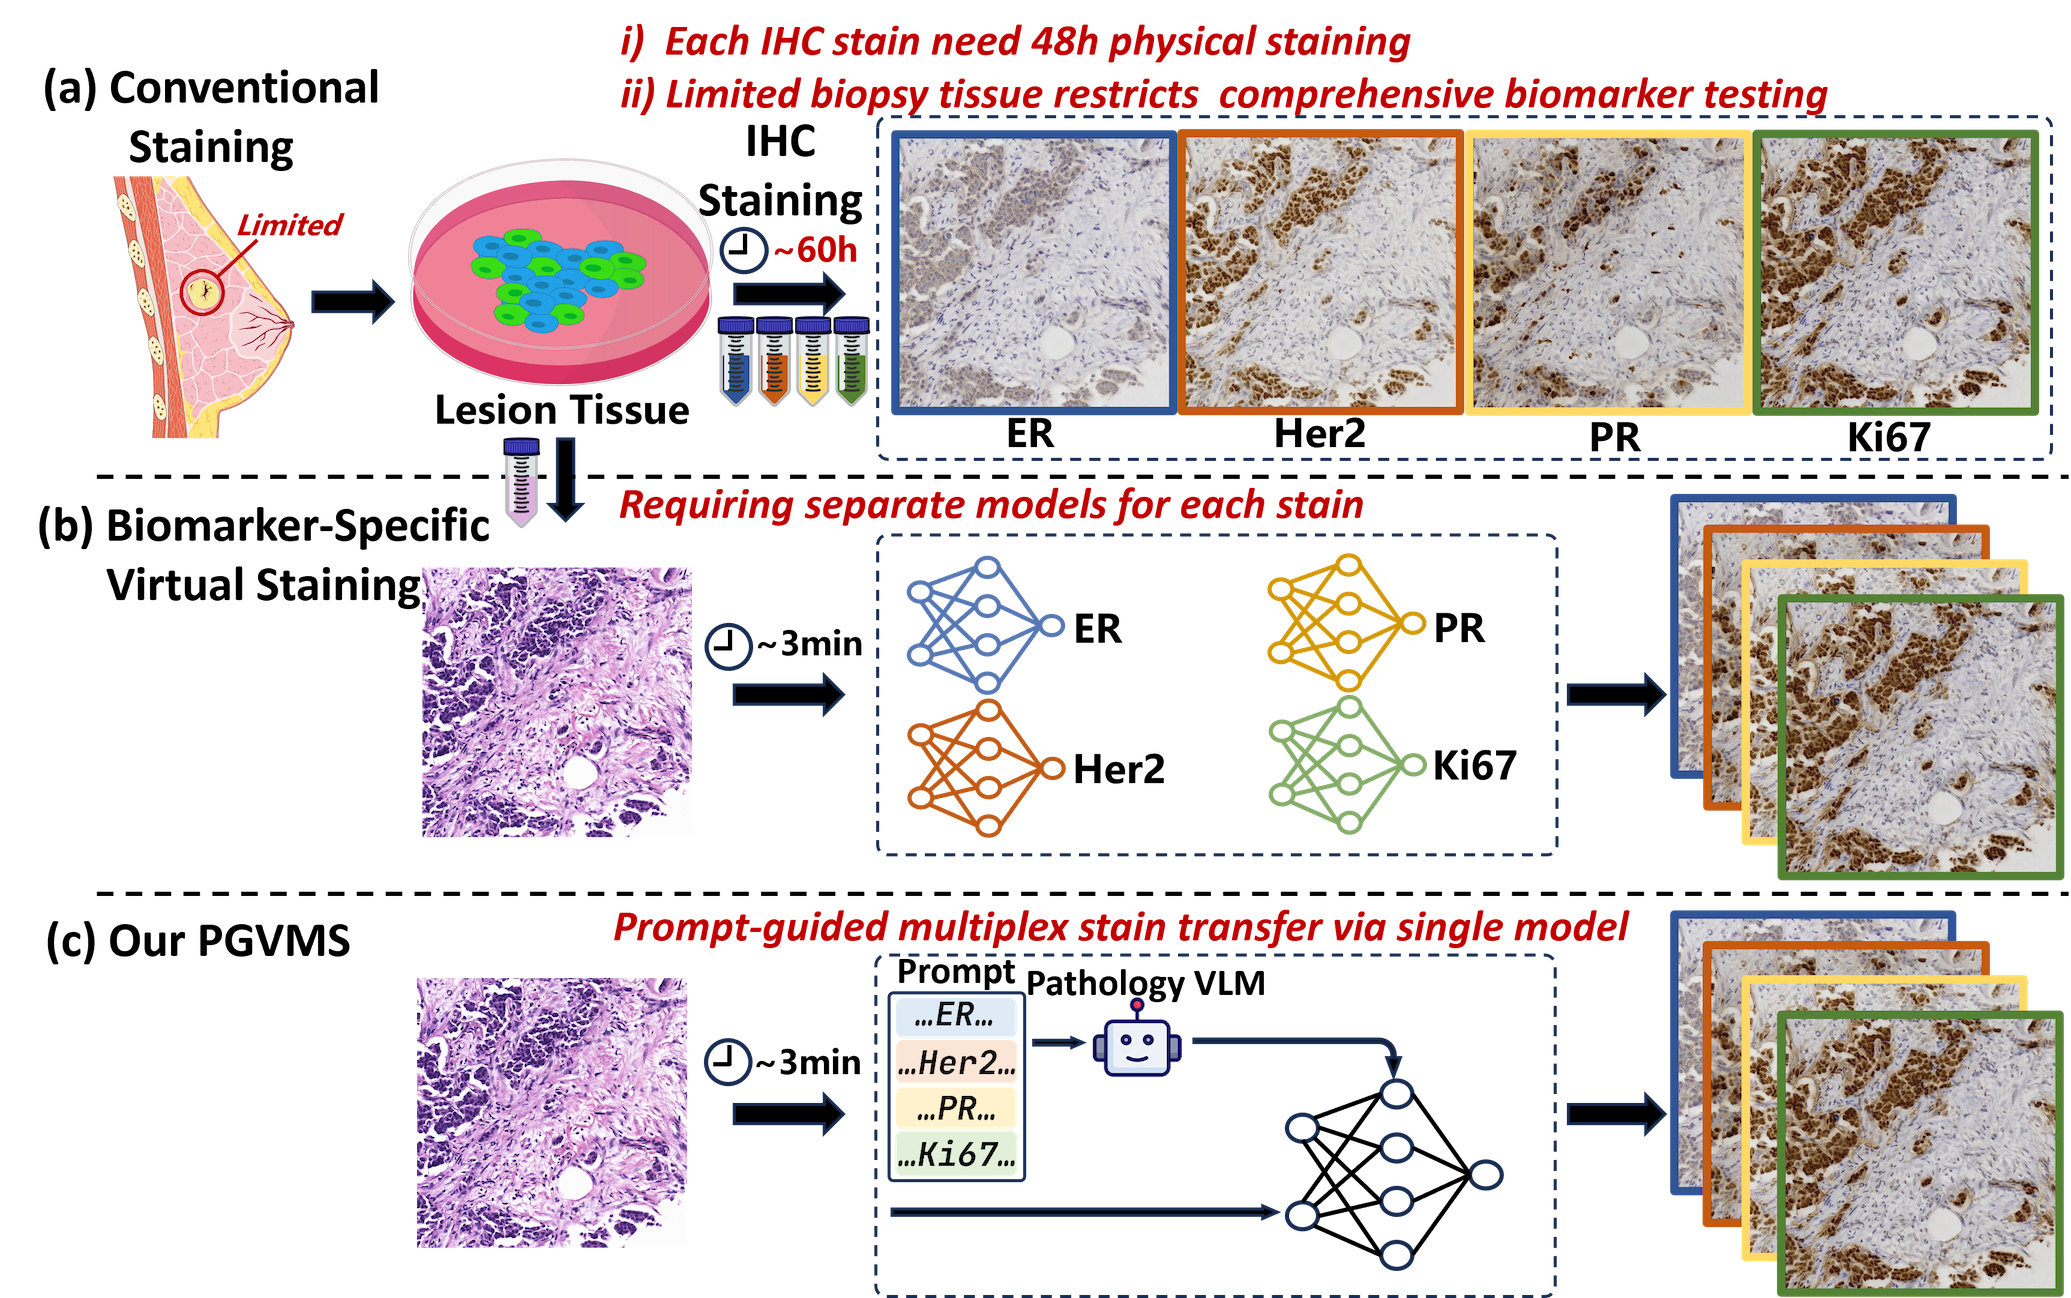
\includegraphics[width=\columnwidth]{image/qin1.png}}
\caption{The comparison of traditional IHC staining and virtual staining workflows. From 
 (a) to (c), they are conventional IHC staining, biomarker-specific virtual staining and our PGVMS.}
\label{intro_1}
\end{figure}


% Virtual staining has emerged as a promising solution as shown in Fig. \ref{intro_1}(b). Virtual staining leverages artificial intelligence techniques to digitally transform H\&E-stained images into IHC-stained images, simulating the appearance of specific biomarkers without the need for physical staining. But conventional approaches that require separate models for each stain type. 


%  - an approach that significantly increases computational costs while failing to capture cross-stain relationships


% To overcome this, our innovative prompt-guided virtual multiplex staining framework (Fig. \ref{intro_1}c) introduces three key advancements: (1) semantic prompt-controlled stain transformation, (2) pathological language modeling to capture inter-marker biological relationships, and (3) a unified architecture generating multiple virtual stains from a single model. Virtual multiplex staining not only preserves critical biomarker correlations but also significantly enhances analytical efficiency, demonstrating particular clinical value in cancer diagnosis. 

% The technology represents a paradigm shift from dedicated single-task models toward unified virtual staining systems.
% where concurrent multi-marker assessment is paramount

% Virtual staining has emerged as a promising solution as shown in Fig. \ref{intro_1}(b). Virtual staining leverages artificial intelligence techniques to digitally transform H\&E-stained images into IHC-stained images, simulating the appearance of specific biomarkers without the need for physical staining. This approach has the potential to significantly reduce the time and cost associated with traditional IHC while maintaining diagnostic accuracy. By enabling rapid and accessible biomarker analysis, virtual staining could revolutionize breast cancer diagnosis \cite{donato2024advancing}. This innovative approach is expected to significantly improve the efficiency of cancer diagnosis as shown in Fig. \ref{intro_1}(c). 


%, particularly in cases where multiple markers like Ki67, ER, PR, and HER2 need to be evaluated simultaneously \cite{hu2023expression}

\begin{figure}[t]
\centerline{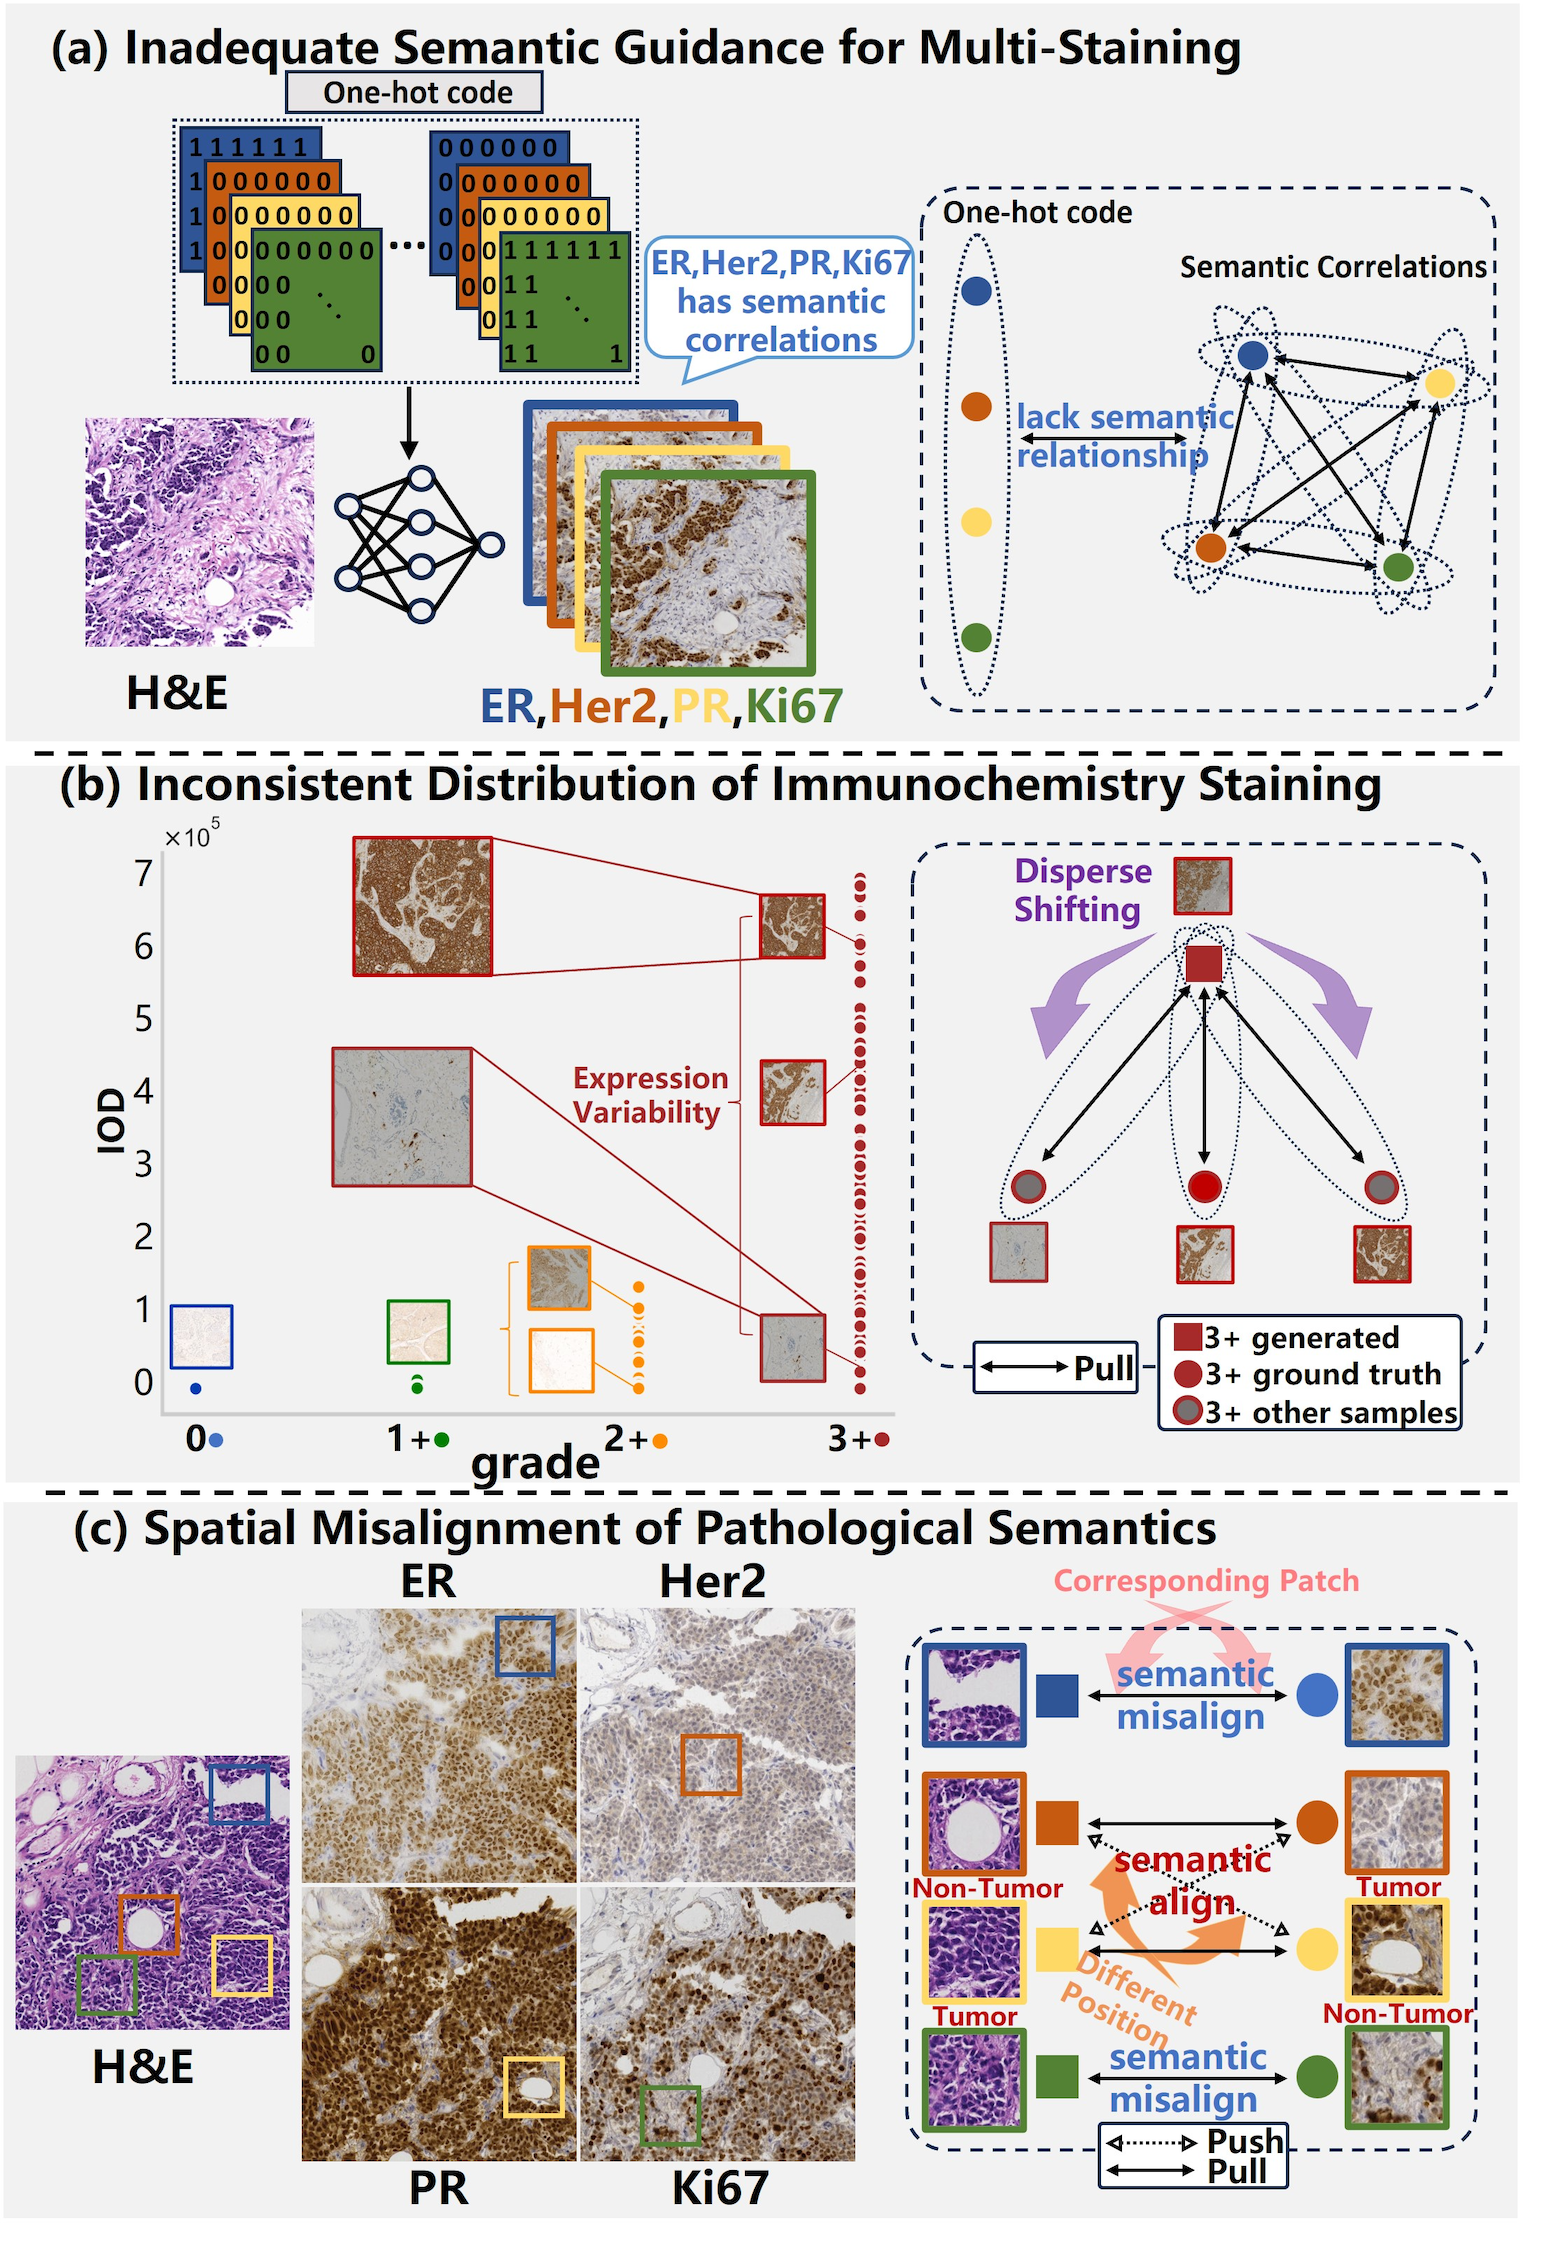
\includegraphics[width=\columnwidth]{image/qin2.png}}
\caption{Three challenges of virtual multi-staining. (a) Inadequate semantic guidance for multi-staining. (b) Inconsistent distribution of immunochemistry staining. (c) Spatial misalignment of pathological semantics.}
\label{intro_2}
\end{figure}

Virtual staining has emerged as a promising computational approach for pathological analysis, as illustrated in Fig. \ref{intro_1}b. This AI-based technique enables digital transformation of H\&E-stained images into IHC representations, simulating biomarker expression patterns without physical staining. However, biomarker-specific virtual staining methods face inefficiency and inconsistency issues, as they require separate models for each stain.
% the current paradigm in virtual staining primarily employs biomarker-specific neural networks, where separate models are independently optimized for individual stain type - an inherently inefficient approach. 

The field of virtual staining has evolved through three stages: (1) initial GAN-based implementations lacking pathological constraints \cite{isola2017image,park2020contrastive,zhu2017unpaired}, (2) subsequently, intermediate solutions incorporating hierarchical semantic information at progressively finer scales (grade-level \cite{zeng2022semi}, patch-level \cite{liu2022bci,zhang2022mvfstain,li2023adaptive}), and (3) some solutions achieving pixel-level precision \cite{liu2021unpaired,peng2024advancing,chen2024pathological}.
% Early approaches directly applied GAN architectures without pathological constraints \cite{isola2017image,park2020contrastive,zhu2017unpaired}, while subsequent advances progressively incorporated hierarchical semantic information from grade-level \cite{zeng2022semi} to patch-level \cite{liu2022bci,zhang2022mvfstain,li2023adaptive} and ultimately pixel-level features with segmentation masks \cite{liu2021unpaired}. 
Significantly, recent breakthroughs enable controlled multi-marker generation through various approaches: Guan et al. \cite{guan2025correlated} developed multi-stain using a shared encoder with four dedicated decoders to exploit inter-marker correlations, while other methods employ one-hot encoding for discrete biomarker selection \cite{lin2022unpaired} or CLIP-based text embedding for prompt control \cite{dubey2024vims}. 


% However, the inherent challenge of virtual multiplex staining lies in the lack of aligned ground truth (GT) pairs for training. Typically, virtual staining GT pairs are obtained from two depth-wise consecutive cuts of the same tissue, which are then stained separately. This approach inevitably prevents pixel-perfect image correspondences due to changes in cell morphology and staining-induced degradation. Therefore how to extract pathological semantic information from the inconsistent GT pairs is the most vital. 


% Both one-hot encoding and CLIP-based prompts fail to capture the cooperative semantic relationships between different stains.
% However, the inherent challenge of virtual staining lies in the lack of aligned ground truth (GT) pairs for training. Typically, virtual staining GT pairs are obtained from two depth-wise consecutive cuts of the same tissue, which are then stained separately. This approach inevitably prevents pixel-perfect image correspondences due to changes in cell morphology and staining-induced degradation. Moreover, due to the irreversibility of the tissue staining process in histopathology, tissue re-staining is usually not performed. As a result, obtaining pixel-level paired data remains a significant challenge. In clinical practice, pathologists often cut consecutive sections from the same tissue and stain them with different markers. While this process ensures global structural consistency between adjacent tissue sections, it introduces cellular and tissue structure variations at the pixel level, leading to weakly paired data.

 % The existing paradigm in computational histopathology predominantly utilizes biomarker-specific neural networks, where discrete models are independently trained to generate virtual staining outputs for singular molecular targets. However, virtual staining GT pairs are obtained from two depth-wise consecutive cuts of the same tissue, which are then stained separately. the inherent challenge of virtual staining lies in the lack of aligned ground truth (GT) pairs for training. Therefore how to extract pathological semantic information from the inconsistent GT pairs is the most important. And they can be viewed as a progressive process aimed at extracting pathological semantic information from inconsistent GT pairs, with the most critical information being at the molecular level. Initially, GAN-based algorithms were directly applied to virtual staining tasks without additional pathological constraints \cite{isola2017image,park2020contrastive,zhu2017unpaired}. More recently, advanced algorithms \cite{zeng2022semi}have begun to incorporate grade-level semantic information to improve the accuracy of virtual staining . Building on this, patch-level semantic information has been integrated to further enhance the preservation of molecular-level semantics \cite{liu2022bci,zhang2022mvfstain,li2023adaptive}. Additionally, pixel-level semantic information has been utilized in conjunction with semantic masks to achieve finer-grained control over the virtual staining process \cite{liu2021unpaired}. This progressive refinement of semantic extraction highlights the ongoing efforts to bridge the gap between computational methods and clinically relevant pathological insights.



% (a) Current virtual staining methods face semantic embedding limitations in one-to-many generation. While one-hot encoding \cite{lin2022unpaired} enables basic multi-marker control, its discrete representation fails to capture biological relationships between stains (e.g., HER2-ER-PR-Ki67 correlations), potentially generating pathologically inconsistent results. Recent advances attempt to address this: Multi-IHC \cite{guan2025correlated} employs shared-encoder architecture to model marker correlations, and CLIP-based methods \cite{dubey2024vims} introduce text-guided generation. However, these approaches still exhibit critical weaknesses - generic CLIP embeddings lack pathology-specific semantics, and multi-decoder designs become prohibitively complex when scaling beyond four markers. An ideal solution would combine biologically-grounded semantic representation with computationally efficient architecture.

% (a) Inefficient Semantic Embedding Transfer: Existing methods fail to introduce sufficient semantic embedding guidance during the process of achieving efficient one-to-many virtual staining. Current approaches typically use one-hot encoding to control one-to-many virtual staining generation, which ignores the inherent semantic relationships between different stains. For example, different markers in IHC staining (e.g., HER2, ER, PR) share biological and tissue expression relationships, yet one-hot encoding treats them as entirely independent categories, leading to the loss of semantic connections between stains. This fixed and disconnected representation weakens the model's ability to preserve semantics during IHC image generation, potentially resulting in biologically incoherent images that reduce their utility in pathological diagnosis and research.





Rethinking the existing methods and challenges of virtual multiplex staining in H\&E to IHC, three significant challenges emerge (Fig. \ref{intro_2}): 
\textbf{(a) Inadequate semantic guidance for multi-staining}: Existing virtual multi-staining methods primarily employ one-hot encoding, which artificially enforces categorical independence among molecular markers while disregarding their inherent biological correlations in tissue expression. Although CLIP-based prompt guidance has been proposed to mitigate this limitation, its general-domain pretraining lacks pathology-specific adaptation, resulting in imprecise histopathological semantic capture. Consequently, current frameworks cannot effectively achieve semantic-aware co-staining generation for multiple biomarkers.
\textbf{(b) Inconsistent distribution of immunochemistry staining}: Current approaches fail to adequately capture fine-grained molecular semantics in pathological images, particularly the precise protein expression levels within specific stained regions. This limitation is especially evident in 3+-grade whole slide images (WSIs), where significant intra-grade variation in protein expression levels exists. By relying solely on coarse grade-level annotations rather than quantifying actual protein expression, existing methods disperse critical molecular-level pathological information, resulting in inconsistent immunochemistry staining distributions between generated and ground-truth IHC images. 
\textbf{(c) Spatial misalignment of pathological semantics}: Typically, virtual staining GT pairs are obtained from two depth-wise consecutive cuts of the same tissue, which are then stained separately. This approach inevitably prevents pixel-perfect image correspondences due to changes in cell morphology and staining-induced degradation. Inherent spatial inconsistencies exist between input images (H\&E) and label images (IHC), meaning that corresponding patches in paired images may contain different normal and tumor cells. Representations with similar semantics may be incorrectly separated and those with opposing semantics may be incorrectly merged. This affects the training efficiency of the model and the semantic accuracy of the generated images.
% (a) Inadequate Semantic Guided for Multi-stain Generation: Current multi-stain approaches predominantly rely on one-hot encoding, which enforces artificial categorical independence among molecular markers (e.g., HER2, ER, PR) and fails to preserve their intrinsic biological correlations in tissue expression. While CLIP-based prompt guidance has been introduced to address this limitation , its general-domain pretraining lacks pathology-specific adaptation, rendering it ineffective at capturing precise histopathological semantics. The current methods fail to achieve effective semantic-guided co-staining generation for multiple molecular markers.
% (b) Insufficient Mining of Pathological Semantics: The representation of molecular-level semantic information, such as protein expression levels, has not been directly extracted for pathological constraints. For instance, the protein expression level of human epidermal growth factor receptor-2 (HER2) varies significantly across samples within 3+-grade whole slide images (WSI). When only grade-level pathological information is preserved, rather than protein expression levels, molecular-level pathological semantics become dispersed, leading to less robust representations. This coarse-grained semantic representation limits the model's potential in precision medicine.
% (c) Spatial Misalignment of Pathological Semantics: Inherent spatial inconsistencies exist between input images (H\&E) and label images (IHC), meaning that corresponding patches in paired images may contain different normal and tumor cells. If similar semantics are assumed in corresponding patches during training, representations with similar semantics may be incorrectly separated, or those with opposing semantics may be incorrectly merged. This affects both the training efficiency of the model and the semantic accuracy of the generated images, ultimately impacting subsequent pathological analysis and diagnosis.


To address the aforementioned challenges, we propose a novel prompt-guided framework for virtual multiplex IHC staining (PGVMS). PGVMS advances virtual multiplex staining by incorporating semantic-preserving mechanisms to maintain critical pathological relationships across different staining modalities. We introduce one novel generator and two innovative learning strategies to tackle the corresponding problems:
(a) For inadequate semantic guidance on multi-stain generation, we propose a pathological semantics-style guided (PSSG) generator  that leverages the CONCH pathology visual language model for prompt-guided stain generation. This approach enables efficient virtual multi-staining by incorporating rich semantic embeddings, ensuring accurate and context-aware transformations from H\&E to multiple IHC stains, such as ER, PR, HER2, and Ki67.
(b) For inconsistent distribution of immunochemistry staining, we directly quantify the protein expression in each IHC-stained image by calculating the optical density in the DAB channel \cite{harms2023multiplex}. This approach preserves molecular-level pathological semantics. {Additionally, we propose a novel focal optical density (FOD) map that adaptively re-weights contributions from protein-expressing regions and normal tissue during quantification, providing a more accurate and robust representation of protein expression levels.}
(c) For spatial misalignment of pathological semantics, we assume that the pathological content of the generated image align with the label. To enhance pathological semantic interaction despite spatial inconsistencies, we facilitate the convergence of pathological features towards cross-corresponding prototypes in both the generated image and the label. This ensures semantic consistency even in the presence of spatial variations.


% During the verification process, we empirically observed that traditional metrics like PSNR and SSIM do not always strictly correlate with high-quality virtual staining results. To address this limitation, we incorporate three pathologically relevant metrics and three awareness metric to better evaluate the clinical utility and accuracy of the generated virtual staining images. These metrics ensure that the results are not only visually appealing but also clinically meaningful.

 % This work extends the conference paper “Pathological Semantics-Preserving Learning for H\&E-to-IHC Virtual Staining” which is published in MICCAI 2024 (Chen et al. \cite{chen2024pathological}). The H\&E-to-IHC virtual staining framework with three major advancements. First, we introduce a novel pathology visual-language model-guided generator that enables prompt-controlled virtual staining, eliminating the previous requirement for stain-specific models. Second, through comprehensive validation, we demonstrate superior pathological consistency in the generated results compared to existing methods. Third, the extended framework achieves robust generalization capabilities for multi-stain prediction from single H\&E inputs in extend datasets. These innovations collectively represent significant improvements over the conference version.
 
 % The IHC virtual staining framework is improved by introducing a novel pathology visual-language model-guided one-to-many generator, which enables controllable IHC virtual staining based on prompts, eliminating the need to train a separate model for each stain as previously required. The conference version is extended with comprehensive experiments, demonstrating that our framework, PGVMS, significantly enhances the pathological consistency of the results. Furthermore, our method achieves efficient one-to-many virtual staining with strong generalization capabilities.


 
% The main contributions of this paper are as follows:
% \begin{itemize}
% \item[•] We propose a PSSG generator that efficiently leverages the pathology visual language model for virtual multi-staining, enabling prompt-guided semantic embedding to generate multiplex IHC stains from a single H\&E image.

% \item[•] We introduce a protein-aware learning strategy (PALS) to extract molecular-level pathological semantics, which directly quantifies and constrains the protein expression levels between the generated image and the label.

% \item[•] {We propose a prototype-consistent learning strategy (PCLS), which establishes a prototypical correlation between the generated high-protein expression regions and the corresponding label, effectively addressing spatial misalignment issues.}


% \item[•] Benchmarking across MIST and IHC4BC datasets reveals our method's dual advantages: superior virtual staining accuracy and efficient multiplex staining with high pathological consistency.  This represents a shift from task-specific architectures to unified virtual staining systems
% % PGVMS represents a paradigm shift from dedicated single-task models toward unified virtual staining systems.
% \end{itemize}

The main contributions of this paper are as follows:
\begin{itemize}
\item[•] \revision{We develop a pathological semantics–style guided (PSSG) generator by integrating a pathology visual language model, enabling prompt-driven semantic embedding for biologically informed multiplex IHC generation.}

\item[•] \revision{To preserve molecular-level pathological semantics, a protein-aware learning strategy (PALS) is introduced to explicitly quantify and constrain protein expression distributions via optical density modeling.}

\item[•] \revision{We further propose a prototype-consistent learning strategy (PCLS) to align high-protein expression prototypes with the label, effectively addressing spatial misalignment.}




\item[•] \revision{Comprehensive experiments on the MIST, IHC4BC, and cross-organ clinical datasets demonstrate that the proposed method achieves state-of-the-art virtual staining accuracy while enabling efficient multiplex IHC generation.}

\end{itemize}




\section{Related works}
\subsection{Image-to-Image Translation}
Image-to-image translation (I2I) aims to transform an input image from a source domain to a target domain while preserving content and transferring style. Early methods like pix2pix \cite{isola2017image} and CycleGAN \cite{zhu2017unpaired} used conditional GANs and cyclic consistency for supervised and unpaired translation, respectively. Park et al. \cite{park2020contrastive} introduced Contrastive Unpaired Translation (CUT), which leverages contrastive learning in a patch-based manner to maximize mutual information between input-output pairs. However, some argue that traditional I2I methods often fail to capture domain-specific details and are limited to one-to-one mappings. For example, Kazemi et al. \cite{kazemi2018unsupervised}  extended CycleGAN to enable one-to-many mappings by learning domain-specific codes, while Almahairi et al. \cite{cyclegan2018learning} proposed augmented CycleGAN for many-to-many multimodal translations. These advancements, with CUT as a key innovation, highlight the importance of balancing content preservation, style transfer, and output diversity in I2I tasks. But these methods are constrained in direct application due to their inability to explicitly preserve pathological semantics.
{In recent years, diffusion-based I2I frameworks have emerged as powerful alternatives, offering stronger generative priors and controllable synthesis. For instance, ControlNet \cite{zhang2023adding} introduces conditional control structures to guide diffusion models with external cues such as edges or segmentation maps, enabling fine-grained structural preservation. UNSB (Unpaired Noise Scheduling Bridge) \cite{kim2023unpaired} formulates I2I as a noise-bridging process between source and target domains, improving domain adaptation and stability. DDBM (Denoising Diffusion Bridge Model) \cite{zhou2023denoising} further extends this concept by explicitly learning domain-conditioned diffusion paths, facilitating faithful translation while maintaining semantic consistency. These diffusion-based paradigms significantly enhance fidelity and controllability, marking a new era for I2I applications, including virtual staining.}
 % Existing image translation methods show promise for virtual staining of pathological images. However, pathological images require high consistency in semantic features. Unsupervised methods lack explicit guidance for preserving pathological semantics, while supervised approaches face pixel misalignment issues in virtual staining datasets. These limitations highlight the need for innovative solutions that can ensure pathological consistency while addressing dataset imperfections.
 
\subsection{Virtual Staining}
Virtual staining using GANs has advanced significantly in recent years. Existing methods focus on extracting pathological semantic information from inconsistent ground truth pairs. For example, Liu et al. \cite{liu2022bci} proposed PyramidP2P, a pyramid pix2pix image generation method, but it requires pixel-level paired data, which is hard to obtain. At the image level, Zeng et al. \cite{zeng2022semi} 
 ensured virtual IHC accuracy with a Pos/Neg classifier. At the patch level, Li et al. \cite{li2023adaptive} introduced ASP, which uses patch-based contrastive learning to tolerate partial data misalignment. At the pixel level, Liu et al. \cite{liu2021unpaired} transformed H\&E to Ki67 using a pathology representation network with expert-annotated labels. Peng et al. \cite{peng2024advancing} extracted tumor information from labeled images using a nuclear density detector to align tumor locations. However, these methods struggle with severe spatial misalignment. To address this, Chen et al. \cite{chen2024pathological} proposed PSPStain, which detects tumor protein expression in patches and uses prototype learning for cross-spatial semantic alignment.
 For virtual multiplex staining, Lin et al. \cite{lin2022unpaired} used style-guided normalization with one-hot encoding to transform one staining type into multiple types. Xiong et al. \cite{xiong2025unpaired} optimizes visual prompts to control content and style. Zhang et al. \cite{zhang2022mvfstain} disentangled style and content to generate multiple staining types while predicting positive signals. Guan et al. \cite{guan2025correlated} developed Multi-IHC, using a shared encoder and four decoders. 
 Dubey et al. \cite{dubey2024vims} introduced VIMs, leveraging CLIP \cite{radford2021learning} for prompt embeddings (e.g., \revision{``CDX2"}) and fine-tuning a diffusion model with LoRA for prompt-controlled multi-virtual staining.
 % Dubey et al. \cite{dubey2024vims} introduced VIMs, which use CLIP embeddings and LoRA-finetuned diffusion models for prompt-controlled multiplex virtual staining.



% \cite{radford2021learning}Xiong et al. \cite{xiong2025unpaired} optimizes visual prompts to control content and style.

% Despite the potential, current methods have limitations. One-hot encoding lacks semantic richness \cite{lin2022unpaired}, and CLIP\cite{dubey2024vims}, not trained on pathology image-text pairs, struggles with IHC embeddings. \cite{zhang2022mvfstain} 不能控制输出哪个染色只能一起输出，Other methods  \cite{liu2022bci,zeng2022semi,li2023adaptive,liu2021unpaired,peng2024advancing,chen2024pathological,guan2025correlated}are computationally inefficient due to a biomarker-specific model. Thus, there is a need for semantic guidance mechanisms to enable multiplex staining.

\revision{Despite their potential, current virtual multiplex staining methods face notable limitations. One-hot encoding approaches \cite{lin2022unpaired} treat molecular markers as independent categories, ignoring biological correlations and limiting semantic richness. Prompt-guided methods, such as Dubey et al. \cite{dubey2024vims}, employ CLIP embeddings with LoRA-finetuned diffusion models for prompt-controlled multiplex staining. However, CLIP is pretrained on general-domain text-image data rather than pathology-specific pairs, so it fails to capture the semantic relationships among different IHC stains. Other methods, such as Zhang et al. \cite{zhang2022mvfstain}, cannot control which stain is generated individually, producing multiple stains simultaneously. Additional approaches \cite{liu2022bci,zeng2022semi,li2023adaptive,liu2021unpaired,peng2024advancing,chen2024pathological,guan2025correlated} rely on biomarker-specific models, which are computationally inefficient and do not scale well for multiple stains. These limitations motivate the need for pathology-aware semantic guidance mechanisms to achieve efficient and biologically consistent multiplex virtual staining.}




\subsection{Pathological Visual Language Model}
In recent years, the development of pathological visual language models (VLMs) has significantly advanced computational pathology, enabling more accurate and efficient analysis of histopathological images. {Among these models, MUSK \cite{xiang2025vision}, PLIP \cite{huang2023visual}, and CONCH \cite{lu2024visual} stand out as notable contributions. MUSK, a vision-language foundation model for precision oncology, achieves state-of-the-art performance by employing a two-stage training paradigm: first, masked learning on 50 million tissue patches and 1 billion textual tokens, followed by contrastive learning on 1 million image-text pairs.} PLIP, on the other hand, utilizes a dataset of over 200,000 pathology image-text pairs sourced from medical Twitter, which enables PLIP to perform tasks like zero-shot classification and cross-modal retrieval. CONCH \cite{lu2024visual} focus on IHC image-text pairs, trained on 1.17 million pathology image-caption pairs. It excels in generating representations for non-H\&E stains, such as IHC and special stains, capturing nuanced relationships between images and text. These models significantly advance computational pathology through large-scale data and multi-modal integration.


% \begin{figure*}[!htbp]
% \centerline{\includegraphics[width=\textwidth]{LaTeX/method.png}}
% \caption{The framework of our PGVMS consists of (a) pathological semantics-style guided generator with two learning strategies: (b) protein-aware learning strategy and (c) prototype-consistent learning strategy.}
% \label{method_1}
% \end{figure*}
\begin{figure*}[!htbp]
\centerline{\includegraphics[width=\textwidth]{image/qin3.png}}
\caption{\revision{The framework of PGVMS. 
(a) Overall architecture of PGVMS, including the pathological semantics--style guided (PSSG) generator and schematic overviews of the protein-aware learning strategy (PALS) and the prototype-consistent learning strategy (PCLS). (b) and (c) show detailed illustrations of PALS and PCLS in the bottom row, highlighting their key components and operations.
}}
\label{method_1}
\end{figure*}



\section{Method}



This section presents the proposed PGVMS framework for generate mIHC images from H\&E images, as shown in Fig. \ref{method_1}. The PGVMS framework comprises three key components designed to achieve optimal virtual staining performance. First, we introduce a pathological semantics-style guided (PSSG) generator that employs prompt-based control to enable efficient multi-stain generation within a single unified model. To ensure pathological fidelity, the framework incorporates two specialized learning strategies: (1) protein-aware learning strategy (PALS) that maintains protein expression consistency across staining modalities, and {(2) prototype-consistent learning strategy (PCLS) that enhances high-protein expression region alignment with established pathological prototypes. }Together, these strategies guarantee the preservation of critical pathological features between virtually generated and physically stained IHC images.




% In this section, we first introduce the pathological semantics-style guided generator. Subsequently, we present the protein-aware learning strategy and prototype-consistent learning strategy.  Finally, we discuss the overall architecture, loss functions, metric and training details.

 



 \subsection{Pathological Semantics-Style Guided Generator}
% In clinical applications, prompt-guided stain generation significantly enhances both the interpretability and practical utility of virtual staining results. Our proposed PSSG generator enables efficient multiple staining by leveraging semantic-rich prompt embeddings (Fig.~\ref{method_1}). This approach not only streamlines the staining workflow but also ensures diagnostic relevance through targeted prompt control.

% Recent advances in pathological foundation models (e.g., PLIP, UNI, CONCH) have demonstrated remarkable multi-modal understanding of medical images and text. CONCH \cite{lu2024visual} distinguishes itself through specialized training on 1.17 million immunohistochemistry (IHC) image-text pairs, establishing a robust cross-modal representation for pathological data. This framework uniquely bridges histomorphological features with immunophenotypic profiles by enabling semantic-based retrieval of specific cellular morphologies. Given its demonstrated efficacy in IHC image-text alignment, we adopt CONCH's pretrained embeddings to initialize our prompt learning module, ensuring pathology-aware feature representation. Given a textual prompt $T$, we first extract the base embedding:


% Building upon recent breakthroughs in pathological foundation models, our framework leverages CONCH's specialized understanding of immunohistochemistry (IHC) data to enable precise stain control. The complete generation pipeline operates through four coordinated stages.

% The process begins with text-derived semantic encoding using CONCH's pretrained text encoder:


Our framework enables efficient multi-stain generation through semantic prompt control, leveraging CONCH's pathology-specific embeddings trained on 1.17 million IHC image-text pairs \cite{lu2024visual}. Given text prompt $T$ (e.g., \revision{``H\&E to Her2 stained image"}), we first extract its base representation:

% Currently, foundational large models have made significant advancements in the field of pathological imaging, such as PLIP, UNI, and {CONCH}. These models focus on different aspects of pathological images and demonstrate exceptional semantic understanding capabilities for both pathological images and text, greatly aiding downstream tasks. To extract semantics from prompts, particularly in the context of IHC staining, we selected CONCH, which is trained on a large dataset of IHC image-text pairs. In the PSSG generation process, we define $T$ as the prompt and first obtain the basic prompt embedding $T_b$ through CONCH:
% Building upon recent advances in pathological foundation models (PLIP, UNI, CONCH), we employ CONCH for prompt embedding due to its specialized training on IHC image-text pairs. Given a textual prompt $T$, we first extract the base embedding:

\begin{equation}
    T_b = \text{CONCH}(T)
\end{equation}
where $T$ represents the natural language prompt and $T_b$ captures its general IHC-related semantics. This foundation model embedding provides crucial prior knowledge about biomarker expression patterns and their pathological significance.

To better align embeddings with individual tumor characteristics, we develop an adaptive image-conditioned bias modulation approach. The H\&E image features $X = G_{enc}(I)$ are processed through dual two pooling branches:

\begin{equation}
    B_i = \text{Conv}(\text{Cat}(\text{MLP}(\text{AvgPool}(X)),\text{MLP}(\text{MaxPool}(X))))
\end{equation}


The average pooling branch captures global tissue architecture, while max pooling emphasizes local cellular abnormalities. Their concatenation and subsequent convolution yield a tumor-specific bias term $B_i$ that refines the prompt embedding:

\begin{equation}
    T_i = T_b + B_i
\end{equation}

{This adjustment ensures the staining process adapts to both the semantic prompt and the unique morphological context of each high-protein expression region.}

The prompt guided style normalization (PGSN) module then modulates the staining process through:
\begin{equation}
    \text{PGSN}(X) = \gamma \cdot (\rho\cdot\text{IN}(X) + (1-\rho)\cdot\text{LN}(X)) + \beta
\end{equation}
where $\gamma,\beta = \text{Conv}(T_i)$ transform semantic embeddings into stain-specific parameters, and $\rho$ automatically balances instance normalization (preserving local staining patterns) against layer normalization (maintaining global tissue structure). This adaptive mixture respects both prompt-derived staining styles and inherent tissue organization.

% where $\gamma,\beta = \text{Conv}(T_i)$ transform the semantic embedding into style parameters, and $\rho$ balances instance vs layer normalization.

After $N$ alternating residual and PGSN blocks, the decoder generates the target stain:
\begin{equation}
    K^F = G_{dec}(\underbrace{\text{PGSN}(\text{Res}(\cdots\text{PGSN}(\text{Res}(X))))}_{N \text{ layers}})
\end{equation}

The complete architecture achieves two key innovations: {First, it bridges general pathological knowledge from foundation models with case-specific high-protein expression characteristics through adaptive prompt tuning. } Second, the hybrid normalization strategy respects both semantic staining directives and biological tissue constraints. 
% Third, the iterative generation process mimics histotechnologists' multi-step staining procedures, yielding diagnostically valid results. 

% This architecture effectively injects prompt-derived semantic styles into the H\&E encoding, enabling precise control over multi-stain generation while maintaining pathological consistency across diverse tissue contexts.
% In clinical practice, guiding the model to generate specific stains using targeted prompts significantly enhances the interpretability and practicality of the results. To achieve efficient virtual multi-IHC staining with a single model, we propose a Pathological Semantics-Style Guided generator, which leverages prompt-based semantic embeddings to generate diverse staining images, as illustrated in Fig.\ref{method_1}. This approach not only streamlines the staining process but also ensures that the generated images align closely with the intended diagnostic goals.

% Currently, foundational large models have made significant advancements in the field of pathological imaging, such as PLIP, UNI, and {CONCH}. These models focus on different aspects of pathological images and demonstrate exceptional semantic understanding capabilities for both pathological images and text, greatly aiding downstream tasks. To extract semantics from prompts, particularly in the context of IHC staining, we selected CONCH, which is trained on a large dataset of IHC image-text pairs. In the PSSG generation process, we define $T$ as the prompt and first obtain the basic prompt embedding $T_b$ through CONCH:
% \begin{equation}
%     T_b = \text{CONCH}(T)
% \end{equation}
% However, the basic prompt embedding for different images, which inherently vary in tumor levels, may constrain the semantic transfer process. This limitation can restrict the model's ability to generalize across diverse image contexts, particularly when dealing with pathological images that exhibit significant variability in tumor characteristics. Such constraints could hinder the model's performance in accurately capturing and transferring semantic information, ultimately impacting its effectiveness in downstream tasks like virtual staining or diagnostic analysis. Therefore, addressing this issue is crucial to enhance the model's adaptability and robustness in handling a wide range of pathological images with varying tumor profiles.
% \begin{equation}\label{image_code}
%     X = G_{enc}(I)
% \end{equation}
% Subsequently, the features are processed through two parallel paths: $Max Pooling$ and $Mean Pooling$, each followed by multiple dense layers. The outputs of these two paths are then concatenated and passed through a $Conv$ to generate the image-specific bias.
% \begin{equation}
%     B_i = Conv(Cat(MLP(AvgPool(X)),MLP(MaxPool(X))))
% \end{equation}
% With the image-specific bias, we get the image-specific prompt embedding$T_i$:
% \begin{equation}
%     T_i = T_b + B_i
% \end{equation}
% To control the stain generation process using the semantically rich prompt embedding $ T_i $, we propose Prompt Guided Style Normalization (PGSN). Specifically, we first process the features obtained from Equation \ref{image_code} through a residual block, followed by a combination of Instance Normalization (IN) and Layer Normalization (LN) with weights $\rho$ and $1-\rho$, respectively. This step generates content-rich features $ X_c $, which facilitate subsequent semantic guidance. 

% Next, the semantically rich prompt embedding $ T_i $ is passed through two separate convolutional layers to extract the style-related scaling factor $\gamma$ and shift factor $\beta$. These style features are then injected into $ X_c $ to produce $ X_s $ for further computation. The PGSN operation is defined as:
% \begin{equation}
%     PGSN(X) = \gamma \cdot (IN(X) \cdot \rho + LN(X) \cdot (1 - \rho)) + \beta
% \end{equation}
% where $\gamma$ and $\beta$ are derived from $ T_i $ via two distinct convolutional layers $Conv(\cdot)$.  $IN$ and $LN$ are instance normalization and layer normalization.

% After alternating between residual blocks and PGSN modules multiple times, the processed features are fed into the decoder $ G_{dec} $ to generate the IHC stain image corresponding to the prompt. This process is expressed as:
% \begin{equation}
%     K^F = G_{dec}\left(\underbrace{PGSN(Res(\cdots PGSN(Res(X))))}_{N \text{ alternating layers}}\right)
% \end{equation}
% where, $Res$ is the $Residual~ Blocks$.

% By the PSSG Generator, the semantic from prompt can be set as a semantic style and embedded in H\&E image encode to guided generate corresponding stain image.




\subsection{Protein-Aware Learning Strategy}
% The DAB chromogen produces a characteristic brown precipitate upon reaction with peroxidase, enabling quantitative analysis of protein expression levels through optical density measurements in the DAB channel.
In IHC staining, target proteins are typically detected through enzyme-conjugated antibodies, with horseradish peroxidase being commonly employed \cite{harms2023multiplex}.
DAB chromogen forms a brown precipitate with peroxidase, allowing protein quantification via DAB channel optical density. Based on these and Chen et al. \cite{chen2024pathological} , PALS initially employs focal optical density mapping to quantify protein distribution in both generated and ground truth images, then applys multi-level protein awareness to enforce biochemical constraints across three hierarchical levels.


\subsubsection{Focal Optical Density Mapping}

Firstly, $K^R$ and $K^F$ undergo subsequent processing to get the FOD.
The optical density (OD) provides a quantitative measure of stain concentration according to the Lambert-Beer law \cite{varghese2014ihc}:
\begin{equation}\label{OD}
    OD_C=-log_{10}(K_C/K_{0,C})=A \ast \boldsymbol{c}_C
\end{equation}
where $K_{0,C}$ and $K_C$ represent the incident and transmitted light intensities respectively for channel $C$, $A$ denotes the stain amount, and $\boldsymbol{c}_C$ is the absorption factor.


Traditional color deconvolution enables DAB stain separation. The stain concentrations are obtained through:

\begin{equation}
{S} = {M}^{-1}\cdot{OD}
\end{equation}
where ${M} \in {R}^{3\times 3}$ is the stain matrix containing absorption coefficients, ${S} \in {R}^{3}$ represents stain concentration vectors. 

Only selecting DAB channel transform to standard OD:

\begin{equation}
D = {M}_{DAB} \cdot {S}_{DAB}
\end{equation}





However, the typically small {protein expression regions relative to normal tissue create a severe class imbalance. To address this, we introduce a focal optical density (FOD) transformation that emphasizes protein expression regions while suppressing normal tissue}:% \cite{ruifrok2001quantification}
\begin{equation}
    {O_C}=(-log_{10}((D_C)/D_{0,C}))^{\alpha}
\end{equation}
where $\alpha > 1$ is a tunable focusing parameter. As shown in Fig.~\ref{method_1}(b), increasing $\alpha$ enhances {protein expression region }emphasis, with $\alpha=1.8$ providing optimal performance in our experiments.

\subsubsection{Multi-Level Protein Awareness}
The multi-level protein awareness (MLPA) loss enforces protein expression consistency between generated ($O^F$) and real ($O^R$) IHC images through a hierarchical constraint framework operating at three biologically meaningful spatial scales:

\textbf{Global Protein Expression Constraint:} 
At the macroscopic level, we constrain the overall staining intensity while allowing for natural biological variations:
\begin{equation}
L_{MLPA-{avg}} =  
\begin{cases}
\left\|\Delta O\right\|_{2}, & \text{if } |\Delta O| \geq \beta \cdot O_{avg}^R \\
0, & \text{if } |\Delta O| < \beta \cdot O_{avg}^R
\end{cases}
\end{equation}
where $\Delta O = O_{avg}^F -O_{avg}^R$ quantifies the mean intensity difference between generated and real images, and $\beta=0.2$ provides a 20\% tolerance threshold that accommodates acceptable clinical variations in staining intensity while preserving diagnostically significant differences.


\textbf{Histogram Distribution Alignment:} The histogram term ensures proper representation of all protein expression levels by comparing normalized intensity distributions across $N_h=20$ bins:
\begin{equation}
     L_{MLPA-{histo}} = \frac{1}{N_h}\sum_{i=1}^{N_h} \left\|O_{histo_i}^F-O_{histo_i}^R\right\|_{2}
\end{equation}
This constraint operates on the complete dynamic range of staining intensities, maintaining proportional representation of clinically relevant expression levels including weak positive regions (0 and 1+), moderate expression (2+), and strong overexpression (3+). The bin-wise comparison prevents common artifacts such as intensity clustering or unrealistic expression distributions.


\textbf{Regional Pattern Consistency:} The regional consistency term preserves local biomarker expression patterns through $N_b=16$ non-overlapping image blocks:
\begin{equation}
     L_{MLPA-{block}} = \frac{1}{N_b}\sum_{i=1}^{N_b} \left\|O_{block_i}^F-O_{block_i}^R\right\|_{2}
\end{equation}
{This spatial constraint ensures proper maintenance of protein expression heterogeneity patterns}, accurate localization of biomarker hotspots, and prevention of unrealistic expression mosaicism. The block-wise comparison mimics pathologists' regional analysis workflow during diagnostic evaluation.


The complete MLPA loss integrates these components:
\begin{equation}
    L_{MLPA} = L_{MLPA-{avg}} + L_{MLPA-{histo}} + L_{MLPA-{block}}
\end{equation}
% In most instances, protein as an antigen is conjugated to an enzyme, such as peroxidase \cite{di2012computer}.
% Among the stains employed for IHC images, the DAB stain yields an intense brown staining when it reacts with the enzyme. Therefore, the fundamental concept behind PALS is to be accurately aware of molecular-level information, specifically protein expression level, by focusing on the DAB channel.

% \noindent{{\textbf{Optical Density Determination:}}} Before presenting PALS, we introduce the optical density (OD). Each stain is characterized by an absorption factor to RGB. Since the OD is proportional to the concentration of the stain, the amount of stain is the factor determining the OD at a wavelength as per the LambertBeer law~\cite{varghese2014ihc}. 
% \begin{equation}\label{OD}
%     OD_C=-log_{10}(I_C/I_{0,C})=A \ast \boldsymbol{c}_C
% \end{equation}

% \noindent where $I_{0, C}$ and $I_C$ denote the light intensity entering and passing the specimen. Subscript $C$ denotes the channel. $A$ is stain amount with absorption factor $\boldsymbol{c}$. 

%  \noindent{\textbf{Focal Optical Density map:}} In this module, we first use the traditional color deconvolution~\cite{ruifrok2001quantification} for stain separation. Then we specifically select DAB stain’s OD values to generate the RGB image (IHC DAB). 

%  In most samples, the tumor area is significantly smaller than the non-tumor area, resulting in a notable imbalance. Hence, training with just the normal OD map Eq.\ref{OD} becomes inefficient as the majority of locations represent easy non-tumor areas, contributing no useful learning signal. Instead, we propose to reshape the map function to down-weight non-tumor area and meanwhile focus training on the tumor area. For FOD, we simulate Eq.\ref{OD} by converting the IHC DAB to grayscale and using the focal calibrated map to assign gray values to positive signal (FOD) as followed:
% \begin{equation}
%     {O_C}=(-log_{10}((I_C)/I_{0,C}))^{\alpha}
% \end{equation}

% \noindent where $O$ is the FOD with tunable focusing
%  parameter $\alpha > 1$.
%  The FOD map is visualized for several values of $\alpha$ in Fig.\ref{fig2}(b). With an increase in the focusing parameter $\alpha$, the de-emphasis of non-tumor areas and the emphasis on tumor areas are enhanced. Among the tested values, $\alpha=1.8$ yields the best results.

% \noindent{\textbf{Multi-Level Protein Awareness:}} For pathology consistency, a Multi-Level Protein Awareness (MLPA) loss is adopted to match fake IHC FOD $O^F$ with real IHC FOD $O^R$. 


%  Initially, we align the average protein expression level and set a tolerance value $\beta$ of 0.2 to account for inherent differences. If the difference in protein expression level is less than $\beta$ multiplied by the average expression level in reference image $O_{avg}^R$, there is no contribution to model learning.

% \begin{equation}
% L_{MLPA-{avg}} =  
% \begin{cases}
% \left\|\Delta O\right\|_{2}, & \text{if } |\Delta O| \geq \beta \cdot O_{avg}^R \\
% 0, & \text{if } |\Delta O| < \beta \cdot O_{avg}^R
% \end{cases}
% \end{equation}
%  \noindent The $O_{avg}$ denotes the average amount of IHC FOD $O$, $ \Delta O = O_{avg}^F - O_{avg}^R $ and $O_{avg}\!=\!\frac{1}{H\!\times\! W} \!\sum_{h=1}^{H}\!\sum_{w=1}^{W}\!O_{h,w}$. 

 
%  Secondly, we divide the FOD range from 0 to $e$ into intervals of $N_h=20$ to ensure consistency in the distribution of protein expression between generated images and labels. 
%  \begin{equation}
%      L_{MLPA-{histo}} = \frac{1}{N_h}\sum_{i=1}^{N_h} \left\|O_{histo_i}^F-O_{histo_i}^R\right\|_{2}
%  \end{equation}
%  \noindent where $O_{histo_i}$ denotes the $i_{th}$ histogram accumulation of the IHC FOD $O$. $O_{histo_i} = \sum_{j=1}^{M_h} O_j$,$if \frac{(i-1) \cdot e}{N_h}<O_j\leq\frac{(i) \cdot e}{N_h}$, where $O_j$ denotes the $j_{th}$ pixel of IHC FOD $O$ and $M_h$ is the number of pixels in the $i_{th}$ histogram. 



%  Finally, we divide the image into $N_b=16$ blocks and independently calculate the average expression amount of each block. This preserves the intensity of expression in specific regions as regularization, referred to as $MLPA-block$.
%  \begin{equation}
%      L_{MLPA-{block}} = \frac{1}{N_b}\sum_{i=1}^{N_b} \left\|O_{block_i}^F-O_{block_i}^R\right\|_{2}
%  \end{equation}
% \noindent where $O_{block_i}$ denotes the $i_{th}$ block average amount of the IHC FOD $O$. $O_{block_i} = \frac{1}{M_b}\sum_{j=1}^{M_b} O_j, if\ position(O_j)\in block_i $ 
% ,where $O_j$ denotes the $j_{th}$ pixel of IHC FOD $O$ and $M_b$ is the number of pixels in the $i_{th}$ block.


% Thus, the overall objective of our MLPA is formulated as follows:
% \begin{equation}
%     L_{MLPA} = L_{MLPA-{avg}} + L_{MLPA-{histo}} + L_{MLPA-{block}}
% \end{equation}

\subsection{Prototype-Consistent Learning Strategy}
% Building upon \cite{zhang2023self}, 

% To addresses the critical challenge of spatial misalignment between generated and reference IHC images, There is  approach is grounded in the fundamental biological principle that tumor content remains intrinsically consistent across different staining modalities of the same tissue specimen. Building on these insights, PCLS first employ Tumor Prototype Extraction to derive representative prototypes and features from both generated and ground truth images, then enforce cross-image prototype consistency through bidirectional alignment.
{To address the challenge of spatial misalignment between generated and reference IHC images, we propose PCLS, a method grounded in the biological principle that protein expression content remains intrinsically consistent across different staining modalities of the adjacent patches. The PCLS first extracts protein prototypes and features from both generated and reference images through protein prototype extraction, then enforces bidirectional cross-image protein prototype consistency.}
\subsubsection{Protein Prototype Extraction}
For each IHC stain type, the prototype extraction process utilizes a corresponding frozen pretrained segmentation UNet to analyze both generated ($K^F$) and real ($K^R$) IHC images through three sequential operations.
% First, the UNet encoder-decoder extracts high-dimensional feature maps $f^F, f^R \in \mathbb{R}^{H\times W \times D}$ from its penultimate layer. 
% Second, the final layer generates pixel-wise probability maps $p_c^F, p_c^R$ through softmax activation, quantifying tumor ($c=1$) versus normal ($c=0$) tissue likelihoods.
% These outputs are then aggregated to derive the final tumor prototypes.

First, the UNet encoder-decoder architecture processes each image to extracts high-dimensional feature maps $f^F, f^R \in \mathbb{R}^{H\times W \times D}$ from its penultimate layer:
\begin{equation}
f^F, f^R  = \text{UNet}_{\text{penultimate}}(K^F,K^R)
\end{equation}

{
Second, the final UNet layer outputs pixel-wise classification probabilities $p_c^F, p_c^R$ through softmax activation, quantifying protein expression ($c=1$) versus normal ($c=0$) tissue likelihoods.}
\begin{equation}
p_c^F, p_c^R = \text{softmax}(\text{UNet}_{\text{final}}(K^F,K^R))
\end{equation}
where $c \in \{\text{protein expression region}, \text{ normal tissue}\}$ indicates the tissue class.

Third, the prototype computation applies confidence-aware feature aggregation by combining the probability maps with their corresponding features:
% The class prototypes are computed through feature aggregation:
\begin{align}
    {q}_c^{{F}}=\frac{\sum_i p_c^F(i)\cdot f^F(i)}{\sum_i p_c^F(i)} ,
    & {q}_c^{{R}}=\frac{\sum_i p_c^R(i)\cdot f^R(i)}{\sum_i p_c^R(i)} 
\end{align}

\subsubsection{Cross-image Protein Prototype Consistency}
The cross-image consistency mechanism enforces bidirectional semantic alignment through cosine similarity measures:
\begin{align}
    \hat{s}_{c}^{FR}=\frac{f^F\cdot{q}_c^R}{\|f^F\|\cdot\left\|{q}_c^R\right\|},
    & \hat{s}_{c}^{RF}=\frac{f^R\cdot{q}_c^F}{\|f^R\|\cdot\left\|{q}_c^F\right\|}
\end{align}

These similarity metrics are converted to probability distributions via softmax normalization:
\begin{align}
    \hat{p}_c^{FR} =\frac{e^{\hat{s}_{c}^{FR}}}{\sum_{c}e^{\hat{s}_{c}^{FR}}},
    & \hat{p}_c^{RF} = \frac{e^{\hat{s}_{c}^{RF}}}{\sum_{c}e^{\hat{s}_{c}^{RF}}}
\end{align}

{The complete cross-protein prototype consistency (CPPC) loss integrates these bidirectional constraints}:
% The cross-image tumor prototype consistency (CTPC) loss enforces agreement between predictions and masks:
\begin{equation}
L_{CPPC} = \frac{1}{C \times H \times W} \sum_{i=1}^{H \times W} \sum_{c=1}^{C} \left( L_{FR}(i, c) + L_{RF}(i, c) \right)
\end{equation}
where the individual loss components measure the deviation between predicted and actual protein regions:
\begin{align*}
L_{FR}(i, c) &= \left\| \hat{p}_c^{FR}(i) - m_c^F(i) \right\|_{2} \\
L_{RF}(i, c) &= \left\| \hat{p}_c^{RF}(i) - m_c^R(i) \right\|_{2}
\end{align*}

\noindent where $m_c^F(i)$ and $ m_c^R(i)$ are derived from $O^F$ and $O^R$, respectively. This formulation simultaneously ensures: (1) cross-modality protein morphology consistency, (2) robustness to staining variations, (3) stain-invariant feature learning, and (4) balanced bidirectional constraint enforcement.

%  Inspired by \cite{zhang2023self}, PCLS effectively preserves pathological semantic consistency even in the presence of spatial misalignment. Specifically, when comparing the generated image $K^F$ with the label $K^R$, it is highly likely that the tumor content within these images remains consistent. Therefore, we calculate the prototype consistency loss $L_{CTPC}$ between them. We derive masks $m_c^F$ and $m_c^R$ by applying the same threshold to fake IHC FOD $O^F$ and real IHC FOD $O^R$.


% \noindent{\textbf{Get Tumor Prototype:}}
% By defining the tumor class and non-tumor class in the IHC image, the prototype of each class refers to the aggregated representation. We pretrain a segmentation UNet with the pseudo mask $m_c^R$ on real IHC images and freeze it to extract tumor semantic. Initially, input IHC image is processed by UNet, yielding a seg probability map as output. Feature maps are then derived from the layer preceding the output layer.
% Let $f^F \in \mathbb{R}^{H\times W \times D}$ represents the feature map of output $K^F$, while $p_c^F(i)$ denotes the probability of pixel $i$ belonging to class $c$. Similarly, $f^R \in \mathbb{R}^{H\times W \times D}$ represents the feature map of label $K^R$, and $p_c^R(i)$ denotes the probability of pixel $i$ belonging to class $c$. Using these feature maps and probability maps, we aggregate class-wise prototypes representing pixel-wise features of tumor and background. The prototypes of output $q_c^F$ and label $q_c^R$ are as followed:
% \begin{align}
%     {q}_c^{{F}}=\frac{\sum_i p_c^F(i)\cdot f^F(i)}{\sum_i p_c^F(i)} ,
%     & {q}_c^{{R}}=\frac{\sum_i p_c^R(i)\cdot f^R(i)}{\sum_i p_c^R(i)} 
% \end{align}



%  \noindent{{\textbf{Cross-image Tumor Prototype Consistency:}}} 
% The feature similarity is calculated based on the output prototype $q_c^F$ and the label prototype $q_c^R$. For semantic interaction, cosine similarity is computed leveraging image features with prototypes from another image. Specifically, $\hat{s}_{c}^{FR}$ and $\hat{s}_{c}^{RF}$ are two cross-image prototypical similarity maps obtained by calculating cosine similarity between the feature map $f^F$, $f^R$ and the prototype vector $q_c^R$, $q_c^F$. These are defined as:
% %\boldsymbol
% \begin{align}
%     \hat{s}_{c}^{FR}=\frac{f^F\cdot{q}_c^R}{\|f^F\|\cdot\left\|{q}_c^R\right\|},
%     & \hat{s}_{c}^{RF}=\frac{f^R\cdot{q}_c^F}{\|f^R\|\cdot\left\|{q}_c^F\right\|}
% \end{align}

% Then, we apply softmax operations to $\hat{s}_c^{FR}$ and $\hat{s}_c^{RF}$ to derive the corresponding cross-image probability prediction $\hat{p}_c^{FR}$ and $\hat{p}_c^{RF}$ respectively:
% %\in \mathbb{R}^{H\times W \times C}
% \begin{align}
%     \hat{p}_c^{FR} =\frac{e^{\hat{s}_{c}^{FR}}}{\sum_{c}e^{\hat{s}_{c}^{FR}}},
%     & \hat{p}_c^{RF} = \frac{e^{\hat{s}_{c}^{RF}}}{\sum_{c}e^{\hat{s}_{c}^{RF}}}
% \end{align}


% The cross-image tumor prototype consistency (CTPC) loss is defined as:
%  % \begin{equation}
%  %     L_{CTPC}=
%  %     \begin{aligned}
%  %     \frac{1}{C\!\times H\!\times W}\!\sum_{i=1}^{H\times W}\!\sum_{c=1}^{C}
%  %     (\left\| \hat{p}_c^{FR}(i)-m_c^F(i)\right\|_{2}\!+\!
%  %     \left\|\hat{p}_c^{RF}(i)-m_c^R(i)\right\|_{2})
%  %     \end{aligned}
%  % \end{equation}
% \begin{equation}
% L_{CTPC} = \frac{1}{C \times H \times W} \sum_{i=1}^{H \times W} \sum_{c=1}^{C} \left( L_{FR}(i, c) + L_{RF}(i, c) \right)
% \end{equation}
% where:
% \begin{align*}
% L_{FR}(i, c) &= \left\| \hat{p}_c^{FR}(i) - m_c^F(i) \right\|_{2} \\
% L_{RF}(i, c) &= \left\| \hat{p}_c^{RF}(i) - m_c^R(i) \right\|_{2}
% \end{align*}


\subsection{Other Loss Function}
{
%Adv
The adversarial loss encourages the generated image $K^F$ to be indistinguishable from the real image $K^R$. It is formulated as:}
{
\begin{equation}
{L}_{{adv}} = 
\mathbb{E}_{K^R} \big[\log D(K^R) \big] +
\mathbb{E}_{K^F} \big[\log (1 - D(K^F)) \big],
\end{equation}
}
{where $D(\cdot)$ denotes the discriminator, $K^F$ is the generated image (fake), and $K^R$ is the real image (ground truth). This loss encourages the generator to produce outputs that are realistic and indistinguishable from real samples.}



%NCE
{
The NCE loss~\cite{oord2018representation,park2020contrastive} aims to preserve content consistency across image translation by maximizing mutual information between corresponding patches in the input and output images. It is formulated as a patch-based InfoNCE objective~\cite{oord2018representation}:}

{
\begin{equation}
{L}_{{NCE}} = - \log \frac{\exp(\hat{z}_Y \cdot z_X / \tau)}
{\exp(\hat{z}_Y \cdot z_X / \tau) + \sum_{n=1}^{N} \exp(\hat{z}_Y \cdot \hat{z}_X^n / \tau)},
\end{equation}
}
{where $\hat{z}_Y$ is the embedding of a patch in the output image (anchor), $z_X$ is the corresponding input patch embedding (positive), $\hat{z}_X^n$ are embeddings of non-corresponding patches (negatives), and $\tau$ is a temperature hyperparameter controlling the sharpness of the softmax distribution.}


%SSIM
{The structural similarity (SSIM) loss encourages the generated image $K^F$ to preserve the structural information of the real image $K^R$:}
{
\begin{equation}
{L}_{{SSIM}} = 1 - \text{SSIM}(K^F, K^R),
\end{equation}
}
{where $\text{SSIM}(\cdot, \cdot)$ computes the structural similarity index between two images. Minimizing ${L}_{{SSIM}}$ promotes preservation of luminance, contrast, and structural patterns in the generated image.}



{
%GP
The gaussian pyramid (GP) loss \cite{liu2022bci} enhances multi-scale consistency between generated and ground truth images, relaxing the strong constraints of the standard L1 loss.}

{The loss at scale $i$ is defined as:}
{
\begin{equation}
S_i = \mathbb{E}_{x,y,z}\left[\|Gaussian_i(K^R) - Gaussian_i(K^F))\|_1\right]
\end{equation}
}
{where $Gaussian_i$ denotes the Gaussian filtering operation at scale $i$, $K^F$ is the output image, $K^R$ is the ground truth.}

{The overall multi-scale loss is formulated as a weighted sum across scales:}
{
\begin{equation}
L_{{GP}} = \sum_{i} \lambda_i S_i
\end{equation}
}
{where $\lambda_i$ represents the weight for scale $i$.}




\subsection{Overall Loss Function}
The overall learning objective is as follows:
\begin{equation}
\begin{aligned}
L_{total} &= L_{adv} + L_{NCE} + \lambda_{M}L_{MLPA} \\
&\quad + \lambda_{C}L_{CPPC} + \lambda_{S}L_{SSIM} + \lambda_{G}L_{GP}
\end{aligned}
\end{equation}
where $L_{MLPA}$, $L_{CPPC}$, $L_{GP}$ focus on pathological consistency, with $L_{GP}$ originating from \cite{liu2022bci}. $L_{adv}, L_{NCE}$, $L_{SSIM}$ contribute to image quality enhancement.

\section{ EXPERIMENTS AND RESULTS}

Our method achieves superior performance on both MIST and IHC4BC datasets for H\&E to IHC multi-stain transfer, enabling efficient prompt-guided virtual staining of multiple biomarkers.
The comparative experimental results show that our method achieve the virtual multiple staining with prompt guided and outperforms other existing methods.
\subsection{Datasets}
\subsubsection{MIST dataset} The MIST dataset~\cite{li2023adaptive} provides precisely aligned H\&E-IHC image pairs for four critical breast cancer biomarkers (Ki67, ER, PR, and HER2). All image patches are non-overlapping 1024×1024 pixels, with substantial training pairs per stain (4,161-4,642) from 56-64 whole slide images (WSIs), each accompanied by a standardized test set of 1,000 image pairs.
\subsubsection{IHC4BC dataset} The IHC4BC dataset~\cite{akbarnejad2023predicting} offers larger-scale aligned H\&E-IHC pairs for the same four biomarkers, containing approximately 90,000 total patches at 1000×1000 resolution. With 52-60 WSIs per stain, it provides significantly more training data (16,995-26,395 pairs per biomarker) while maintaining the same 1,000-pair test set standardization. 

Both datasets maintain overall structural alignment despite minor local deformations, serving as comprehensive benchmarks for computational pathology research.
% \subsubsection{MIST Dataset}



% \begin{table*}[ht]
%   \centering
%   \setlength\tabcolsep{5pt}
%   % \fontsize{8}{9}\selectfont
%   \renewcommand{\arraystretch}{1}
%   \caption{COMPARISON OF VIRTUAL STAINING PERFORMANCE ON \textbf{MIST} DATASET. THE BEST AND SECOND BEST SCORES ARE IN BOLD AND UNDERLINE, RESPECTIVELY.}
%   \label{tab:all_datasets}

%   \resizebox{\textwidth}{!}{
%     \begin{tabular}{c|cc|cc|cc|cc|cc|cc}
%       \Xhline{1.5pt} 
%       \multirow{3}{*}{Method} & 
%       \multicolumn{6}{c|}{HER2} & \multicolumn{6}{c}{ER} \\
%       \cline{2-13}
%       & \multicolumn{2}{c|}{Pathology} & \multicolumn{2}{c|}{Quality (reference)} & \multicolumn{2}{c|}{Perception} & 
%       \multicolumn{2}{c|}{Pathology} & \multicolumn{2}{c|}{Quality (reference)} & \multicolumn{2}{c}{Perception} \\
%       \cline{2-13}
%       & IOD${\times10^7}$ & Pearson-R$\uparrow$ & PSNR$\uparrow$ & SSIM$\uparrow$ & FID$\downarrow$ & DISTS$\downarrow$  & IOD${\times10^7}$ & Pearson-R$\uparrow$ & PSNR$\uparrow$ & SSIM$\uparrow$ & FID$\downarrow$ & DISTS$\downarrow$ \\
%       \hline
%       CycleGAN~\cite{zhu2017unpaired} & 
%       +4.5848 & 0.1995 & 12.20 & 0.1588 & 63.91 & 0.2864 & 
%       -1.6250 & 0.2916 & 13.25 & 0.2187 & 54.14 & 0.2730 \\
      
%       Pix2Pix~\cite{isola2017image} & 
%       -2.5782 & 0.2986 & 12.98 & 0.1676 & 84.37 & 0.2699 & 
%       -5.8452 & 0.6307 & \textbf{14.73} & 0.2200 & 90.64 & 0.3050 \\
      
%       CUT~\cite{park2020contrastive} & 
%       -2.9478 & 0.7164 & 13.90 & 0.1680 & 53.30 & 0.2641 & 
%       -4.5073 & 0.5841 & 14.22 & \textbf{0.2201} & 45.81 & 0.2630 \\
      
%       ASP~\cite{li2023adaptive} & 
%       -5.7422 & 0.0659 & 14.18 & \textbf{0.2004} & 50.85 & 0.2517 & 
%       -4.5875 & 0.4802 & 14.21 & 0.2178 & 54.79 & 0.2705 \\
      
%       PyramidP2P~\cite{liu2022bci} & 
%       -4.5285 & 0.6894 & \textbf{14.91} & 0.1995 & 91.35 & 0.2628 & 
%       -4.2775 & 0.7418 & 14.21 & 0.2023 & 92.93 & 0.2703 \\
      
%       TDKStain~\cite{peng2024advancing} &
%       -3.1244 & 0.8147 & 14.7620 & 0.1901 & 62.8442 & 0.2515 & 
%       -2.6321 & 0.8466 & 14.3451 & 0.2113 & 46.7817 & 0.2483 \\
      
%       PSPStain~\cite{chen2024pathological} & 
%       -2.5491 & 0.8303 & 14.19 & 0.1876 & \textbf{41.36} & 0.2541 & 
%       -2.0571 & 0.8763 & 14.57 & 0.2143 & 39.89 & 0.2431 \\

%       DDBM~\cite{zhou2023denoising} &
%       -6.4420 & -0.0228 & \textbf{14.7785} & \textbf{0.2156} & 201.5442 & 0.3426 &
%       -7.6428 & 0.1280 & \textbf{14.6963} & 0.2368 & 191.6672 & 0.3336 \\
      
%       UNSB~\cite{kim2023unpaired} &
%       -1.8809 & 0.3141 & 13.2797 & 0.2121 & 54.6514 & 0.3015 &
%       -1.5399 & 0.3981 & 13.3957 & \textbf{0.2452} & 39.1415 & 0.2955 \\
%       ControlNet~\cite{zhang2023adding} &
%       +3.2796 & 0.0080 & 8.6754 & 0.1658 & 121.8161 & 0.3882 &
%       +19.2318 & 0.0505 & 8.4172 & 0.1564 & 155.9284 & 0.3499 \\
      
%       VIMs~\cite{dubey2024vims} & 
%       -7.0886 & 0.3049 & 13.9114 & 0.1953 & 130.5218 & 0.3077 &
%       -2.9966 & 0.0434 & 14.1536 & 0.1969 & 97.3877 & 0.2979 \\
%       UMDST & 
%     1.7366 & 0.1037 & 12.6934 & \textbf{0.2181} & 71.4340 & 0.3124 &
%    -1.5309 & 0.4156 & 13.6387 & \textbf{0.2528} & 59.9249 & 0.3122 \\
%       %  vims & 
%       % -7.0886 & 0.3049 & 13.9114 & 0.1953 & 130.5218 & 0.3077 &
%       % -2.9966 & 0.0434 & 14.1536 & 0.1969 & 97.3877 & 0.2979 \\
      
%       % controlnet &
%       % +3.2796 & 0.0080 & 8.6754 & 0.1658 & 121.8161 & 0.3882 &
%       % +19.2318 & 0.0505 & 8.4172 & 0.1564 & 155.9284 & 0.3499 \\

%       % DDBM\_real &
%       % -6.4420 & -0.0228 & 14.7785 & 0.2156 & 201.5442 & 0.3426 &
%       % -7.6428 & 0.1280 & 14.6963 & 0.2368 & 191.6672 & 0.3336 \\
      

     
%      PGVMS & 
%       \textbf{-0.4390} & \textbf{0.8548} & 13.92 & 0.1769 & 44.43 & \textbf{0.2336} & 
%       \textbf{-0.5193} & \textbf{0.8902} & 14.36 & 0.2072 & \textbf{36.58} & \textbf{0.2299} \\
%       \hline
      
%       \multirow{3}{*}{Method} & 
%       \multicolumn{6}{c|}{PR} & \multicolumn{6}{c}{Ki67} \\
%       \cline{2-13}
%       & \multicolumn{2}{c|}{Pathology} & \multicolumn{2}{c|}{Quality} & \multicolumn{2}{c|}{Perception} & 
%       \multicolumn{2}{c|}{Pathology} & \multicolumn{2}{c|}{Quality} & \multicolumn{2}{c}{Perception} \\
%       \cline{2-13}
%        & IOD${\times10^7}$ & Pearson-R$\uparrow$ & PSNR$\uparrow$ & SSIM$\uparrow$ & FID$\downarrow$  & DISTS$\downarrow$ 
%        & IOD${\times10^7}$ & Pearson-R$\uparrow$ & PSNR$\uparrow$ & SSIM$\uparrow$ & FID$\downarrow$ & DISTS$\downarrow$ \\
%       \hline
%      CycleGAN~\cite{zhu2017unpaired} & 
%       -6.1662 & 0.2229 & 13.85 & 0.2040 & 75.45 & 0.2736 & 
%       -2.6220 & 0.2726 & 13.91 & 0.2186 & 46.15 & 0.2538 \\
    
%       Pix2Pix~\cite{isola2017image} & 
%       -5.8785 & 0.7201 & \textbf{15.06} & 0.2338 & 80.49 & 0.3101 & 
%       -2.0715 & 0.5560 & 14.61 & 0.2360 & 93.80 & 0.2568 \\
      
%       CUT~\cite{park2020contrastive} & 
%       -2.8106 & 0.7032 & 14.35 & 0.2209 & 41.23 & 0.2601 & 
%       -2.2291 & 0.4878 & 14.41 & 0.2095 & 42.07 & 0.2520 \\
      
%       ASP~\cite{li2023adaptive} & 
%       -5.7499 & 0.5557 & 14.12 & 0.2111 & 47.85 & 0.2547 & 
%       -2.3507 & 0.4562 & 14.59 & 0.2286 & 50.93 & 0.2462 \\
      
%       PyramidP2P~\cite{liu2022bci} & 
%       -5.9274 & 0.7318 & 14.26 & 0.2097 & 85.67 & 0.2718 & 
%       -0.6542 & 0.5877 & 13.95 & 0.2231 & 87.85 & \textbf{0.2417} \\

%       TDKStain~\cite{peng2024advancing} &
%       -2.5365 & 0.8658 & 14.7783 & 0.2320 & 56.2217 & 0.2534 &
%       -1.0361 & 0.7473 & 14.6585 & 0.2391 & 58.5757 & 0.2454 \\
      
%       PSPStain~\cite{chen2024pathological} & 
%       -3.5771 & 0.8661 & 14.88 & \textbf{0.2347} & 38.35 & 0.2454 & 
%       \textbf{-0.0671} & 0.7718 & 14.26 & \textbf{0.2415} & 37.57 & 0.2607 \\
      
       
      
%       DDBM~\cite{zhou2023denoising} &
%       -6.4651 & 0.4206 & 13.4919 & 0.2242 & 168.8190 & 0.3087 &
%       -1.8336 & 0.4149 & 14.1996 & 0.2357 & 158.1006 & 0.2909 \\
      
%       UNSB~\cite{kim2023unpaired} &
%       -1.2455 & 0.3906 & 13.7457 & \textbf{0.2572} & 41.3750 & 0.3136 &
%       \textbf{-0.3999} & 0.3981 & 14.1265 & 0.2722 & \textbf{33.2999} & 0.2836 \\
%        ControlNet~\cite{zhang2023adding} &
%       +5.6869 & 0.0928 & 9.0790 & 0.1508 & 136.1356 & 0.3710 &
%       +6.4306 & 0.2751 & 10.2877 &\textbf{ 0.2831} & 292.4799 & 0.3955 \\
%       VIMs~\cite{dubey2024vims} & 
%       -4.2534 & 0.0341 & 13.3384 & 0.1591 & 115.3529 & 0.3069 &
%       -6.0985 & 0.2202 & 13.7166 & 0.1906 & 110.7464 & 0.3002 \\
%       UMDST & 
%    -1.7874 & 0.4968 & 13.7066 & \textbf{0.2515} & 59.4099 & 0.3039 &
%     \textbf{+0.7868} & 0.2642 & 13.8163 & \textbf{0.2595} & 94.9168 & 0.3174 \\
%       % ===================== 追加部分 =====================
% % (直接复制到原表格 PGVMS 那行之后)
        
%       % vims & 
%       % -4.2534 & 0.0341 & 13.3384 & 0.1591 & 115.3529 & 0.3069 &
%       % -6.0985 & 0.2202 & 13.7166 & 0.1906 & 110.7464 & 0.3002 \\



%       % controlnet &
%       % +5.6869 & 0.0928 & 9.0790 & 0.1508 & 136.1356 & 0.3710 &
%       % +6.4306 & 0.2751 & 10.2877 & 0.2831 & 292.4799 & 0.3955 \\

%       % DDBM\_real &
%       % -6.4651 & 0.4206 & 13.4919 & 0.2242 & 168.8190 & 0.3087 &
%       % -1.8336 & 0.4149 & 14.1996 & 0.2357 & 158.1006 & 0.2909 \\
% % =====================

      
%       PGVMS & 
%       \textbf{+0.7815} & \textbf{0.9126} & 14.25 & 0.2000 & \textbf{34.91} & \textbf{0.2300} & 
%       -1.1125 & \textbf{0.8018} & \textbf{14.83} & 0.2285 & \textbf{36.36} & 0.2439 \\
%       \Xhline{1.5pt} 
%     \end{tabular}
%   }
% \end{table*}

\begin{table*}[ht]
  \centering
  \setlength\tabcolsep{4.5pt}
  \renewcommand{\arraystretch}{1}
  \caption{\revision{COMPARISON OF VIRTUAL STAINING PERFORMANCE ON \textbf{MIST} DATASET. 
  THE BEST SCORES ARE IN BOLD. 
  MODELS ARE GROUPED INTO ONE-TO-ONE AND ONE-TO-MANY CATEGORIES.
}}
  \label{tab:all_datasets}

  \resizebox{\textwidth}{!}{
    \begin{tabular}{c|c|cc|cc|cc|cc|cc|cc}
      \Xhline{1.5pt}
      \multirow{3}{*}{Type} & 
      \multirow{3}{*}{Method} & 
      \multicolumn{6}{c|}{HER2} & \multicolumn{6}{c}{ER} \\
      \cline{3-14}
      & & \multicolumn{2}{c|}{Quality (reference)} & \multicolumn{2}{c|}{Pathology} & \multicolumn{2}{c|}{Perception} & 
      \multicolumn{2}{c|}{Quality (reference)} & \multicolumn{2}{c|}{Pathology} & \multicolumn{2}{c}{Perception} \\
      \cline{3-14}
      & & PSNR$\uparrow$ & SSIM$\uparrow$ & IOD$_{\times10^7}$ & Pearson-R$\uparrow$ & FID$\downarrow$ & DISTS$\downarrow$ &
      PSNR$\uparrow$ & SSIM$\uparrow$ & IOD$_{\times10^7}$ & Pearson-R$\uparrow$ & FID$\downarrow$ & DISTS$\downarrow$ \\
      \hline
      % ------------------- One-to-one models -------------------
      \multirow{9}{*}{One-to-one} 
      & CycleGAN~\cite{zhu2017unpaired} & 
      12.2042 & 0.1588 & +4.5848 & 0.1995 & 63.8952 & 0.2864 & 
      13.2516 & 0.2187 & -1.6250 & 0.2916 & 54.1309 & 0.2730 \\
      
      & Pix2Pix~\cite{isola2017image} & 
      12.9840 & 0.1676 & -2.5782 & 0.2986 & 84.3667 & 0.2699 & 
      \textbf{14.7293} & 0.2200 & -5.8452 & 0.6307 & 90.6261 & 0.3050 \\
      
      & CUT~\cite{park2020contrastive} & 
      13.8998 & 0.1680 & -2.9478 & 0.7164 & 53.2911 & 0.2641 & 
      14.2172 & 0.2201 & -4.5073 & 0.5841 & 45.8074 & 0.2630 \\
      
      & ASP~\cite{li2023adaptive} & 
      14.1841 & 0.2004 & -5.7422 & 0.0659 & 50.8364 & 0.2517 & 
      14.2088 & 0.2178 & -4.5875 & 0.4802 & 54.7745 & 0.2705 \\
      
      & PyramidP2P~\cite{liu2022bci} & 
      \textbf{14.9122} & 0.1995 & -4.5285 & 0.6894 & 91.3455 & 0.2628 & 
      14.2062 & 0.2023 & -4.2775 & 0.7418 & 92.9292 & 0.2703 \\
      
      & TDKStain~\cite{peng2024advancing} &
      14.7620 & 0.1901 & -3.1244 & 0.8147 & 62.8442 & 0.2515 & 
      14.3451 & 0.2113 & -2.6321 & 0.8466 & 46.7817 & 0.2483 \\
      
      & PSPStain~\cite{chen2024pathological} & 
      14.1948 & 0.1876 & -2.5491 & 0.8303 & \textbf{41.3439} & 0.2541 & 
      14.5718 & 0.2143 & -2.0571 & 0.8763 & 39.8844 & 0.2431 \\

      & DDBM~\cite{zhou2023denoising} &
      14.7785 & 0.2156 & -6.4420 & -0.0228 & 201.5442 & 0.3426 &
      14.6963 & 0.2368 & -7.6428 & 0.1280 & 191.6672 & 0.3336 \\
      
      & UNSB~\cite{kim2023unpaired} &
      13.2797 & 0.2121 & -1.8809 & 0.3141 & 54.6514 & 0.3015 &
      13.3957 & 0.2452 & -1.5399 & 0.3981 & 39.1415 & 0.2955 \\
      
      
      \Xhline{0.8pt}
      % ------------------- One-to-many models -------------------
      \rowcolor{gray!10}
    % \multirow{4}{*}{\cellcolor{gray!10}One-to-many} 
    & \cellcolor{gray!10}ControlNet~\cite{zhang2023adding} &
    8.6754 & 0.1658 & +3.2796 & 0.0080 & 121.8161 & 0.3882 &
    8.4172 & 0.1564 & +19.2318 & 0.0505 & 155.9284 & 0.3499 \\
    \rowcolor{gray!10}
    & \cellcolor{gray!10}VIMs~\cite{dubey2024vims} & 
    13.9114 & 0.1953 & -7.0886 & 0.3049 & 130.5218 & 0.3077 &
    14.1536 & 0.1969 & -2.9966 & 0.0434 & 97.3877 & 0.2979 \\
    \rowcolor{gray!10}
    & \cellcolor{gray!10}UMDST~\cite{lin2022unpaired} & 
    12.6934 & \textbf{0.2181} & 1.7366 & 0.1037 & 71.4340 & 0.3124 &
    13.6387 & \textbf{0.2528} & -1.5309 & 0.4156 & 59.9249 & 0.3122 \\
   
    \rowcolor{gray!10}
   \multirow{-4}{*}{One-to-many}  & \cellcolor{gray!10}PGVMS & 
    13.9246 & 0.1769 & \textbf{-0.4390} & \textbf{0.8548} & 44.4247 & \textbf{0.2336} &
    14.3583 & 0.2072 & \textbf{-0.5193} & \textbf{0.8902} & \textbf{36.5734} & \textbf{0.2299} \\

      \hline
      % ========================= Second half =========================
      \multirow{3}{*}{Type} & 
      \multirow{3}{*}{Method} & 
      \multicolumn{6}{c|}{PR} & \multicolumn{6}{c}{Ki67} \\
      \cline{3-14}
      & & \multicolumn{2}{c|}{Quality (reference)} & \multicolumn{2}{c|}{Pathology} & \multicolumn{2}{c|}{Perception} & 
      \multicolumn{2}{c|}{Quality (reference)} & \multicolumn{2}{c|}{Pathology} & \multicolumn{2}{c}{Perception} \\
      \cline{3-14}
      & & PSNR$\uparrow$ & SSIM$\uparrow$ & IOD$_{\times10^7}$ & Pearson-R$\uparrow$ & FID$\downarrow$  & DISTS$\downarrow$ 
      & PSNR$\uparrow$ & SSIM$\uparrow$ & IOD$_{\times10^7}$ & Pearson-R$\uparrow$ & FID$\downarrow$ & DISTS$\downarrow$ \\
      \hline
      % ------------------- One-to-one models -------------------
      
      \multirow{9}{*}{One-to-one} 
      & CycleGAN~\cite{zhu2017unpaired} & 
      13.8537 & 0.2040 & -6.1662 & 0.2229 & 75.4442 & 0.2736 & 
      13.9144 & 0.2186 & -2.6220 & 0.2726 & 46.1386 & 0.2538 \\
      
      & Pix2Pix~\cite{isola2017image} & 
      \textbf{15.0557} & 0.2338 & -5.8785 & 0.7201 & 80.4802 & 0.3101 & 
      14.6090 & 0.2360 & -2.0715 & 0.5560 & 93.7772 & 0.2568 \\
      
      & CUT~\cite{park2020contrastive} & 
      14.3480 & 0.2209 & -2.8106 & 0.7032 & 41.2165 & 0.2601 & 
      14.4081 & 0.2095 & -2.2291 & 0.4878 & 42.0596 & 0.2520 \\
      
      & ASP~\cite{li2023adaptive} & 
      14.1200 & 0.2111 & -5.7499 & 0.5557 & 47.8368 & 0.2547 & 
      14.5852 & 0.2286 & -2.3507 & 0.4562 & 50.9120 & 0.2462 \\
      
      & PyramidP2P~\cite{liu2022bci} & 
      14.2600 & 0.2097 & -5.9274 & 0.7318 & 85.6816 & 0.2718 & 
      13.9477 & 0.2231 & -0.6542 & 0.5877 & 87.8460 & \textbf{0.2417} \\

      & TDKStain~\cite{peng2024advancing} &
      14.7783 & 0.2320 & -2.5365 & 0.8658 & 56.2217 & 0.2534 &
      14.6585 & 0.2391 & -1.0361 & 0.7473 & 58.5757 & 0.2454 \\
      
      & PSPStain~\cite{chen2024pathological} & 
      14.8824 & 0.2347 & -3.5771 & 0.8661 & 38.3390 & 0.2454 & 
      14.2602 & 0.2415 & \textbf{-0.0671} & 0.7718 & 37.5574 & 0.2607 \\
      
      & DDBM~\cite{zhou2023denoising} &
      13.4919 & 0.2242 & -6.4651 & 0.4206 & 168.8190 & 0.3087 &
      14.1996 & 0.2357 & -1.8336 & 0.4149 & 158.1006 & 0.2909 \\
      
      & UNSB~\cite{kim2023unpaired} &
      13.7457 & \textbf{0.2572} & -1.2455 & 0.3906 & 41.3750 & 0.3136 &
      14.1265 & 0.2722 & -0.3999 & 0.3981 & \textbf{33.2999} & 0.2836 \\
      
       \Xhline{0.8pt}
      % ------------------- One-to-many models -------------------
      \rowcolor{gray!10}
      
      & ControlNet~\cite{zhang2023adding} &
      9.0790 & 0.1508 & +5.6869 & 0.0928 & 136.1356 & 0.3710 &
      10.2877 & \textbf{0.2831} & +6.4306 & 0.2751 & 292.4799 & 0.3955 \\
       \rowcolor{gray!10}
      & VIMs~\cite{dubey2024vims} & 
      13.3384 & 0.1591 & -4.2534 & 0.0341 & 115.3529 & 0.3069 &
      13.7166 & 0.1906 & -6.0985 & 0.2202 & 110.7464 & 0.3002 \\
     \rowcolor{gray!10}
      & UMDST~\cite{lin2022unpaired} & 
      13.7066 & 0.2515 & -1.7874 & 0.4968 & 59.4099 & 0.3039 &
      13.8163 & 0.2595 & +0.7868 & 0.2642 & 94.9168 & 0.3174 \\
     
       \rowcolor{gray!10}
      \multirow{-4}{*}{One-to-many}& PGVMS & 
      14.2510 & 0.2000 & \textbf{+0.7815} & \textbf{0.9126} & \textbf{34.9099} & \textbf{0.2300} & 
      \textbf{14.8344} & 0.2285 & -1.1125 & \textbf{0.8018} & 36.3537 & 0.2439 
      \\
      \Xhline{1.5pt} 
    \end{tabular}
  }
\end{table*}

% \begin{table*}[ht]
%   \centering
%   \setlength\tabcolsep{5pt}
%   \renewcommand{\arraystretch}{1}
%   \caption{COMPARISON OF VIRTUAL STAINING PERFORMANCE ON \textbf{MIST} DATASET. THE BEST AND SECOND BEST SCORES ARE IN BOLD AND UNDERLINE, RESPECTIVELY.}
%   \label{tab:all_datasets}

%   \resizebox{\textwidth}{!}{
%     \begin{tabular}{c|cc|cc|cc|cc|cc|cc}
%       \Xhline{1.5pt} 
%       \multirow{3}{*}{Method} & 
%       \multicolumn{6}{c|}{HER2} & \multicolumn{6}{c}{ER} \\
%       \cline{2-13}
%       & \multicolumn{2}{c|}{Quality (reference)} & \multicolumn{2}{c|}{Pathology} & \multicolumn{2}{c|}{Perception} & 
%       \multicolumn{2}{c|}{Quality (reference)} & \multicolumn{2}{c|}{Pathology} & \multicolumn{2}{c}{Perception} \\
%       \cline{2-13}
%       & PSNR$\uparrow$ & SSIM$\uparrow$ & IOD${\times10^7}$ & Pearson-R$\uparrow$ & FID$\downarrow$ & DISTS$\downarrow$ &
%       PSNR$\uparrow$ & SSIM$\uparrow$ & IOD${\times10^7}$ & Pearson-R$\uparrow$ & FID$\downarrow$ & DISTS$\downarrow$ \\
%       \hline
%       CycleGAN~\cite{zhu2017unpaired} & 
%       12.2042 & 0.1588 & +4.5848 & 0.1995 & 63.8952 & 0.2864 & 
%       13.2516 & 0.2187 & -1.6250 & 0.2916 & 54.1309 & 0.2730 \\
      
%       Pix2Pix~\cite{isola2017image} & 
%       12.9840 & 0.1676 & -2.5782 & 0.2986 & 84.3667 & 0.2699 & 
%       \textbf{14.7293} & 0.2200 & -5.8452 & 0.6307 & 90.6261 & 0.3050 \\
      
%       CUT~\cite{park2020contrastive} & 
%       13.8998 & 0.1680 & -2.9478 & 0.7164 & 53.2911 & 0.2641 & 
%       14.2172 & 0.2201 & -4.5073 & 0.5841 & 45.8074 & 0.2630 \\
      
%       ASP~\cite{li2023adaptive} & 
%       14.1841 & 0.2004 & -5.7422 & 0.0659 & 50.8364 & 0.2517 & 
%       14.2088 & 0.2178 & -4.5875 & 0.4802 & 54.7745 & 0.2705 \\
      
%       PyramidP2P~\cite{liu2022bci} & 
%       \textbf{14.9122} & 0.1995 & -4.5285 & 0.6894 & 91.3455 & 0.2628 & 
%       14.2062 & 0.2023 & -4.2775 & 0.7418 & 92.9292 & 0.2703 \\
      
%       TDKStain~\cite{peng2024advancing} &
%       14.7620 & 0.1901 & -3.1244 & 0.8147 & 62.8442 & 0.2515 & 
%       14.3451 & 0.2113 & -2.6321 & 0.8466 & 46.7817 & 0.2483 \\
      
%       PSPStain~\cite{chen2024pathological} & 
%       14.1948 & 0.1876 & -2.5491 & 0.8303 & \textbf{41.3439} & 0.2541 & 
%       14.5718 & 0.2143 & -2.0571 & 0.8763 & 39.8844 & 0.2431 \\

%       DDBM~\cite{zhou2023denoising} &
%       14.7785 & 0.2156 & -6.4420 & -0.0228 & 201.5442 & 0.3426 &
%       14.6963 & 0.2368 & -7.6428 & 0.1280 & 191.6672 & 0.3336 \\
      
%       UNSB~\cite{kim2023unpaired} &
%       13.2797 & 0.2121 & -1.8809 & 0.3141 & 54.6514 & 0.3015 &
%       13.3957 & 0.2452 & -1.5399 & 0.3981 & 39.1415 & 0.2955 \\
%       ControlNet~\cite{zhang2023adding} &
%       8.6754 & 0.1658 & +3.2796 & 0.0080 & 121.8161 & 0.3882 &
%       8.4172 & 0.1564 & +19.2318 & 0.0505 & 155.9284 & 0.3499 \\
      
%       VIMs~\cite{dubey2024vims} & 
%       13.9114 & 0.1953 & -7.0886 & 0.3049 & 130.5218 & 0.3077 &
%       14.1536 & 0.1969 & -2.9966 & 0.0434 & 97.3877 & 0.2979 \\
%       UMDST~\cite{lin2022unpaired} & 
%       12.6934 & \textbf{0.2181} & 1.7366 & 0.1037 & 71.4340 & 0.3124 &
%       13.6387 & \textbf{0.2528} & -1.5309 & 0.4156 & 59.9249 & 0.3122 \\
      
%      PGVMS & 
%       13.9246 & 0.1769 & \textbf{-0.4390} & \textbf{0.8548} & 44.4247 & \textbf{0.2336} & 
%       14.3583 & 0.2072 & \textbf{-0.5193} & \textbf{0.8902} & \textbf{36.5734} & \textbf{0.2299} \\
%       \hline
      
%       \multirow{3}{*}{Method} & 
%       \multicolumn{6}{c|}{PR} & \multicolumn{6}{c}{Ki67} \\
%       \cline{2-13}
%       & \multicolumn{2}{c|}{Quality (reference)} & \multicolumn{2}{c|}{Pathology} & \multicolumn{2}{c|}{Perception} & 
%       \multicolumn{2}{c|}{Quality (reference)} & \multicolumn{2}{c|}{Pathology} & \multicolumn{2}{c}{Perception} \\
%       \cline{2-13}
%       & PSNR$\uparrow$ & SSIM$\uparrow$ & IOD${\times10^7}$ & Pearson-R$\uparrow$ & FID$\downarrow$  & DISTS$\downarrow$ 
%       & PSNR$\uparrow$ & SSIM$\uparrow$ & IOD${\times10^7}$ & Pearson-R$\uparrow$ & FID$\downarrow$ & DISTS$\downarrow$ \\
%       \hline
%      CycleGAN~\cite{zhu2017unpaired} & 
%       13.8537 & 0.2040 & -6.1662 & 0.2229 & 75.4442 & 0.2736 & 
%       13.9144 & 0.2186 & -2.6220 & 0.2726 & 46.1386 & 0.2538 \\
    
%       Pix2Pix~\cite{isola2017image} & 
%       \textbf{15.0557} & 0.2338 & -5.8785 & 0.7201 & 80.4802 & 0.3101 & 
%       14.6090 & 0.2360 & -2.0715 & 0.5560 & 93.7772 & 0.2568 \\
      
%       CUT~\cite{park2020contrastive} & 
%       14.3480 & 0.2209 & -2.8106 & 0.7032 & 41.2165 & 0.2601 & 
%       14.4081 & 0.2095 & -2.2291 & 0.4878 & 42.0596 & 0.2520 \\
      
%       ASP~\cite{li2023adaptive} & 
%       14.1200 & 0.2111 & -5.7499 & 0.5557 & 47.8368 & 0.2547 & 
%       14.5852 & 0.2286 & -2.3507 & 0.4562 & 50.9120 & 0.2462 \\
      
%       PyramidP2P~\cite{liu2022bci} & 
%       14.2600 & 0.2097 & -5.9274 & 0.7318 & 85.6816 & 0.2718 & 
%       13.9477 & 0.2231 & -0.6542 & 0.5877 & 87.8460 & \textbf{0.2417} \\

%       TDKStain~\cite{peng2024advancing} &
%       14.7783 & 0.2320 & -2.5365 & 0.8658 & 56.2217 & 0.2534 &
%       14.6585 & 0.2391 & -1.0361 & 0.7473 & 58.5757 & 0.2454 \\
      
%       PSPStain~\cite{chen2024pathological} & 
%       14.8824 & 0.2347 & -3.5771 & 0.8661 & 38.3390 & 0.2454 & 
%       14.2602 & 0.2415 & \textbf{-0.0671} & 0.7718 & 37.5574 & 0.2607 \\
      
%       DDBM~\cite{zhou2023denoising} &
%       13.4919 & 0.2242 & -6.4651 & 0.4206 & 168.8190 & 0.3087 &
%       14.1996 & 0.2357 & -1.8336 & 0.4149 & 158.1006 & 0.2909 \\
      
%       UNSB~\cite{kim2023unpaired} &
%       13.7457 & \textbf{0.2572} & -1.2455 & 0.3906 & 41.3750 & 0.3136 &
%       14.1265 & 0.2722 & -0.3999 & 0.3981 & \textbf{33.2999} & 0.2836 \\
%       ControlNet~\cite{zhang2023adding} &
%       9.0790 & 0.1508 & +5.6869 & 0.0928 & 136.1356 & 0.3710 &
%       10.2877 & \textbf{0.2831} & +6.4306 & 0.2751 & 292.4799 & 0.3955 \\
%       VIMs~\cite{dubey2024vims} & 
%       13.3384 & 0.1591 & -4.2534 & 0.0341 & 115.3529 & 0.3069 &
%       13.7166 & 0.1906 & -6.0985 & 0.2202 & 110.7464 & 0.3002 \\
%       UMDST \cite{lin2022unpaired} & 
%       13.7066 & 0.2515 & -1.7874 & 0.4968 & 59.4099 & 0.3039 &
%       13.8163 & 0.2595 & +0.7868 & 0.2642 & 94.9168 & 0.3174 \\
      
%       PGVMS & 
%       14.2510 & 0.2000 & \textbf{+0.7815} & \textbf{0.9126} & \textbf{34.9099} & \textbf{0.2300} & 
%       \textbf{14.8344} & 0.2285 & -1.1125 & \textbf{0.8018} & 36.3537 & 0.2439 \\
%       \Xhline{1.5pt} 
%     \end{tabular}
%   }
% \end{table*}



\begin{table*}[ht]
  \centering
  \setlength\tabcolsep{5pt}
  \renewcommand{\arraystretch}{1}
  \caption{\revision{COMPARISON OF VIRTUAL STAINING PERFORMANCE ON \textbf{IHC4BC} DATASET. THE BEST SCORES ARE IN BOLD. MODELS ARE GROUPED INTO ONE-TO-ONE AND ONE-TO-MANY CATEGORIES.
}}
  \label{tab:ihc4bc_results}

  \resizebox{\textwidth}{!}{
    \begin{tabular}{c|c|cc|cc|cc|cc|cc|cc}
      \Xhline{1.5pt} 
       \multirow{3}{*}{Type} &\multirow{3}{*}{Method} & 
      \multicolumn{6}{c|}{HER2} & \multicolumn{6}{c}{ER} \\
      \cline{3-14}
      && \multicolumn{2}{c|}{Quality (reference)} & \multicolumn{2}{c|}{Pathology} & \multicolumn{2}{c|}{Perception} & 
      \multicolumn{2}{c|}{Quality (reference)} & \multicolumn{2}{c|}{Pathology} & \multicolumn{2}{c}{Perception} \\
      \cline{3-14}
      && PSNR$\uparrow$ & SSIM$\uparrow$ & IOD$_{\times10^8}$ & Pearson-R$\uparrow$ & FID$\downarrow$ & DISTS$\downarrow$ & PSNR$\uparrow$ & SSIM$\uparrow$ & IOD$_{\times10^7}$ & Pearson-R$\uparrow$ & FID$\downarrow$ & DISTS$\downarrow$ \\
      \hline
     \multirow{9}{*}{One-to-one} 
      &CycleGAN~\cite{zhu2017unpaired} & 10.1229 & 0.0930 & +1.9836 & 0.3071 & 143.8269 & 0.3385 & 17.3148 & 0.4406 & +0.8744 & 0.3878 & 50.9366 & 0.2545 \\
      &Pix2Pix~\cite{isola2017image} & 11.3910 & 0.1228 & -0.9739 & 0.6214 & 117.3533 & 0.3027 & 20.7537 & 0.4931 & -1.0956 & 0.2171 & 129.9073 & 0.3050 \\
      &CUT~\cite{park2020contrastive} & 10.9131 & 0.1227 & -1.2030 & -0.0613 & 63.3108 & 0.2657 & 19.4466 & 0.4745 & -1.0011 & 0.0705 & 41.8358 & 0.2618 \\
      &ASP~\cite{li2023adaptive} & 11.2034 & 0.1245 & -1.1742 & -0.0988 & 63.9972 & 0.2658 & 19.5277 & 0.4834 & -0.6886 & 0.1810 & 37.9753 & 0.2644 \\
      &PyramidP2P~\cite{liu2022bci} & 10.8870 & 0.1325 & -0.5059 & 0.4234 & 113.6700 & 0.3612 & \textbf{21.2933} & \textbf{0.5606} & -1.3231 & 0.1230 & 121.3450 & 0.4019 \\
      &TDKStain~\cite{peng2024advancing} & 11.0847 & 0.1263 & -0.4522 & 0.7451 & 72.6141 & \textbf{0.2498} & 19.6842 & 0.4652 & -0.5041 & 0.5925 & 50.3415 & 0.2529 \\
      &PSPStain~\cite{chen2024pathological} & 11.1210 & 0.1213 & -0.5439 & 0.7022 & 57.0579 & 0.2585 & 18.6233 & 0.4240 & -0.2761 & 0.7651 & 39.6011 & 0.2586 \\
           
        &DDBM~\cite{zhou2023denoising} & \textbf{11.7847} & 0.1136 & -1.2303 & -0.0095 & 206.7112 & 0.4091 & 20.5214 & 0.4749 & -1.3201 & 0.0103 & 290.9201 & 0.3711 \\
      &UNSB~\cite{kim2023unpaired} & 11.0874 & 0.1392 & -0.6440 & 0.1654 & 54.7004 & 0.3155 & 19.4668 & 0.4963 & -0.6459 & 0.3130 & 61.3214 & 0.3151 \\
       \Xhline{0.8pt}
      % ------------------- One-to-many models -------------------
      \rowcolor{gray!10}
     & ControlNet~\cite{zhang2023adding}  & 7.9736 & 0.1028 & +0.6942 & 0.2747 & 143.5401 & 0.3846 & 7.4402 & 0.2908 & +25.7725 & 0.0412 & 235.9315 & 0.4063 \\
      \rowcolor{gray!10}
     & VIMs~\cite{dubey2024vims} & 11.3224 & 0.1226 & -1.0667 & 0.0945 & 86.0438 & 0.3693 & 17.4837 & 0.4001 & -0.8389 & 0.3534 & 90.6424 & 0.3068 \\
      \rowcolor{gray!10}
      &  UMDST~\cite{lin2022unpaired} & 
   11.1742 & \textbf{0.1449} & -0.3930 & 0.4135 & 65.5618 & 0.3183 &
   20.5402 & 0.5346 & -1.1084 & 0.1270 & 63.3261 & 0.3448 \\

    % vims &
    %   11.3224 & 0.1226 & -1.0667 & 0.0945 & 86.0438 & 0.3693 &
    %   17.4837 & 0.4001 & -0.8389 & 0.3534 & 90.6424 & 0.3068 \\

    %   controlnet &
    %   7.9736 & 0.1028 & +0.6942 & 0.2747 & 143.5401 & 0.3846 &
    %   7.4402 & 0.2908 & +25.7725 & 0.0412 & 235.9315 & 0.4063 \\

    %   DDBM\_real &
    %   11.7847 & 0.1136 & -1.2303 & -0.0095 & 206.7112 & 0.4091 &
    %   20.5214 & 0.4749 & -1.3201 & 0.0103 & 290.9201 & 0.3711 \\
     
     \rowcolor{gray!10}
    \multirow{-4}{*}{One-to-many}&  PGVMS & 11.0508 & 0.1234 & \textbf{-0.3262} & \textbf{0.7751} & \textbf{53.3853} & 0.2552 & 19.7848 & 0.4750 & \textbf{-0.1098} & \textbf{0.7940} & \textbf{36.8306} & \textbf{0.2326} \\
      \hline
      
       \multirow{3}{*}{Type} &\multirow{3}{*}{Method} & 
      \multicolumn{6}{c|}{PR} & \multicolumn{6}{c}{Ki67} \\
      \cline{3-14}
      && \multicolumn{2}{c|}{Quality (reference)} & \multicolumn{2}{c|}{Pathology} & \multicolumn{2}{c|}{Perception} & 
      \multicolumn{2}{c|}{Quality (reference)} & \multicolumn{2}{c|}{Pathology} & \multicolumn{2}{c}{Perception} \\
      \cline{3-14}
      && PSNR$\uparrow$ & SSIM$\uparrow$ & IOD$_{\times10^7}$ & Pearson-R$\uparrow$ & FID$\downarrow$ & DISTS$\downarrow$ & PSNR$\uparrow$ & SSIM$\uparrow$ & IOD$_{\times10^7}$ & Pearson-R$\uparrow$ & FID$\downarrow$ & DISTS$\downarrow$ \\
      \hline
     \multirow{9}{*}{One-to-one} 
     & CycleGAN~\cite{zhu2017unpaired} & 17.9551 & 0.4544 & +1.3643 & 0.2339 & 66.0757 & 0.3113 & 18.7757 & 0.3840 & +0.8227 & 0.6277 & 52.5754 & 0.2328 \\
     & Pix2Pix~\cite{isola2017image} & 23.9329 & 0.5556 & -0.5986 & 0.1558 & 116.1813 & 0.2702 & 20.5521 & 0.4413 & -0.4839 & 0.2138 & 140.2222 & 0.2914 \\
      &CUT~\cite{park2020contrastive} & 19.0278 & 0.4882 & +0.6367 & 0.2133 & 47.5413 & 0.3153 & 17.2823 & 0.3017 & -0.5802 & 0.1187 & 114.3944 & 0.3063 \\
     & ASP~\cite{li2023adaptive} & 23.3897 & 0.5454 & -0.5677 & -0.0954 & 42.3880 & 0.2575 & 19.1923 & 0.3849 & -0.2544 & 0.5686 & 27.0728 & 0.2272 \\
      &PyramidP2P~\cite{liu2022bci} & 24.1510 & \textbf{0.6187} & -0.5892 & 0.0479 & 87.7714 & 0.3378 & 20.7354 & \textbf{0.4895} & -0.4475 & 0.3627 & 63.2432 & 0.3150 \\
    &  TDKStain~\cite{peng2024advancing} & 21.9699 & 0.5236 & -0.2936 & 0.0073 & 64.9066 & 0.2739 & 19.4341 & 0.4014 & \textbf{-0.0994} & 0.8735 & 38.1665 & 0.2302 \\
    &  PSPStain~\cite{chen2024pathological} & 23.8481 & 0.5544 & -0.5586 & 0.5877 & 43.8625 & 0.2503 & 18.9546 & 0.3966 & +0.4443 & 0.8744 & 32.2626 & 0.2539 \\
      % ===================== 追加部分 =====================
% （直接复制到 PGVMS 后面）



    &  DDBM~\cite{zhou2023denoising} & 22.5329 & 0.5293 & -5.6605 & 0.0136 & 239.2746 & 0.3284 & 19.1372 & 0.3744 & -0.3313 & 0.5537 & 120.2547 & 0.3166 \\
     & UNSB~\cite{kim2023unpaired} & 23.7180 & 0.5957 & -0.5131 & 0.2865 & 42.2145 & 0.3052 & 20.5115 & 0.4523 & -0.4590 & 0.7595 & 35.9533 & 0.2905 \\
        \Xhline{0.8pt}
      % ------------------- One-to-many models -------------------
      \rowcolor{gray!10}
     & ControlNet~\cite{zhang2023adding}  & 8.3349 & 0.2686 & +9.6558 & 0.0084 & 259.7857 & 0.4424 & 8.8441 & 0.2168 & +6.5673 & 0.6417 & 252.8057 & 0.4164 \\
     \rowcolor{gray!10}
    &  VIMs~\cite{dubey2024vims} & \textbf{24.2096} & 0.5438 & -0.6146 & 0.0075 & 112.9235 & 0.3357 & \textbf{20.7378} & 0.3930 & -0.5592 & 0.5227 & 84.4047 & 0.3316 \\
      \rowcolor{gray!10}
       &  UMDST~\cite{lin2022unpaired}&
    22.5452 & 0.5795 & -0.4066 & 0.0761 & 45.6025 & 0.3120 &
    20.1732 & 0.4651 & -0.4733 & 0.5237 & 56.5546 & 0.3003 \\
    
    \rowcolor{gray!10}

      % vims &
      % 24.2096 & 0.5438 & -0.6146 & 0.0075 & 112.9235 & 0.3357 &
      % 20.7378 & 0.3930 & -0.5592 & 0.5227 & 84.4047 & 0.3316 \\

      % controlnet &
      % 8.3349 & 0.2686 & +9.6558 & 0.0084 & 259.7857 & 0.4424 &
      % 8.8441 & 0.2168 & +6.5673 & 0.6417 & 252.8057 & 0.4164 \\

      % DDBM\_real &
      % 22.5329 & 0.5293 & -5.6605 & 0.0136 & 239.2746 & 0.3284 &
      % 19.1372 & 0.3744 & -0.3313 & 0.5537 & 120.2547 & 0.3166 \\
% =====================

    \multirow{-4}{*}{One-to-many} & PGVMS & 22.4371 & 0.5388 & \textbf{-0.0499} & \textbf{0.7084} & \textbf{40.6377} & \textbf{0.2495} & 20.3849 & 0.4191 & -0.2256 & \textbf{0.8913} & \textbf{24.4450} & \textbf{0.2208} \\
      \Xhline{1.5pt} 
    \end{tabular}
  }
\end{table*}

% \begin{table*}[ht]
%   \centering
%   \setlength\tabcolsep{5pt}
%   \renewcommand{\arraystretch}{1}
%   \caption{COMPARISON OF STAIN TRANSFER PERFORMANCE ON IHC4BC DATASET. THE BEST AND SECOND BEST SCORES ARE IN BOLD AND UNDERLINE, RESPECTIVELY.}
%   \label{tab:ihc4bc_results}

%   \resizebox{\textwidth}{!}{
%     \begin{tabular}{c|cc|cc|cc|cc|cc|cc}
%       \Xhline{1.5pt} 
%       \multirow{3}{*}{Method} & 
%       \multicolumn{6}{c|}{HER2} & \multicolumn{6}{c}{ER} \\
%       \cline{2-13}
%       & \multicolumn{2}{c|}{Pathology} & \multicolumn{2}{c|}{Quality} & \multicolumn{2}{c|}{Perception} & 
%       \multicolumn{2}{c|}{Pathology} & \multicolumn{2}{c|}{Quality} & \multicolumn{2}{c}{Perception} \\
%       \cline{2-13}
%       & IOD$\times10^8$ & Pearson-R$\uparrow$ & PSNR$\uparrow$ & SSIM$\uparrow$ & FID$\downarrow$ & DISTS$\downarrow$ & IOD$\times10^7$ & Pearson-R$\uparrow$ & PSNR$\uparrow$ & SSIM$\uparrow$ & FID$\downarrow$ & DISTS$\downarrow$ \\
%       \hline
%       CycleGAN~\cite{zhu2017unpaired} & +1.9836 & 0.3071 & 10.1229 & 0.0930 & 143.8269 & 0.3385 & +0.8744 & 0.3878 & 17.3148 & 0.4406 & 50.9366 & 0.2545 \\
%       Pix2Pix~\cite{isola2017image} & -0.9739 & 0.6214 & \textbf{11.3910} & 0.1228 & 117.3533 & 0.3027 & -1.0956 & 0.2171 & 20.7537 & 0.4931 & 129.9073 & 0.3050 \\
%       CUT~\cite{park2020contrastive} & -1.2030 & -0.0613 & 10.9131 & 0.1227 & 63.3108 & 0.2657 & -1.0011 & 0.0705 & 19.4466 & 0.4745 & 41.8358 & 0.2618 \\
%       ASP~\cite{li2023adaptive} & -1.1742 & -0.0988 & 11.2034 & 0.1245 & 63.9972 & 0.2658 & -0.6886 & 0.1810 & 19.5277 & 0.4834 & 37.9753 & 0.2644 \\
%       Pyramid~\cite{liu2022bci} & -0.5059 & 0.4234 & 10.8870 & \textbf{0.1325} & 113.6700 & 0.3612 & -1.3231 & 0.1230 & \textbf{21.2933} & \textbf{0.5606} & 121.3450 & 0.4019 \\
%       TDKStain~\cite{peng2024advancing} & -0.4522 & 0.7451 & 11.0847 & 0.1263 & 72.6141 & \textbf{0.2498} & -0.5041 & 0.5925 & 19.6842 & 0.4652 & 50.3415 & 0.2529 \\
%       PSPStain~\cite{chen2024pathological} & -0.5439 & 0.7022 & 11.1210 & 0.1213 & 57.0579 & 0.2585 & -0.2761 & 0.7651 & 18.6233 & 0.4240 & 39.6011 & 0.2586 \\
%       PGVMS & \textbf{-0.3262} & \textbf{0.7751} & 11.0508 & 0.1234 & \textbf{53.3853} & 0.2552 & \textbf{-0.1098} & \textbf{0.7940} & 19.7848 & 0.4750 & \textbf{36.8306} & \textbf{0.2326} \\
%       \hline
      
%       \multirow{3}{*}{Method} & 
%       \multicolumn{6}{c|}{PR} & \multicolumn{6}{c}{Ki67} \\
%       \cline{2-13}
%       & \multicolumn{2}{c|}{Pathology} & \multicolumn{2}{c|}{Quality} & \multicolumn{2}{c|}{Perception} & 
%       \multicolumn{2}{c|}{Pathology} & \multicolumn{2}{c|}{Quality} & \multicolumn{2}{c}{Perception} \\
%       \cline{2-13}
%       & IOD$\times10^7$ & Pearson-R$\uparrow$ & PSNR$\uparrow$ & SSIM$\uparrow$ & FID$\downarrow$ & DISTS$\downarrow$ & IOD$\times10^7$ & Pearson-R$\uparrow$ & PSNR$\uparrow$ & SSIM$\uparrow$ & FID$\downarrow$ & DISTS$\downarrow$ \\
%       \hline
%       CycleGAN~\cite{zhu2017unpaired} & +1.3643 & 0.2339 & 17.9551 & 0.4544 & 66.0757 & 0.3113 & +0.8227 & 0.6277 & 18.7757 & 0.3840 & 52.5754 & 0.2328 \\
%       Pix2Pix~\cite{isola2017image} & -0.5986 & 0.1558 & 23.9329 & 0.5556 & 116.1813 & 0.2702 & -0.4839 & 0.2138 & 20.5521 & 0.4413 & 140.2222 & 0.2914 \\
%       CUT~\cite{park2020contrastive} & +0.6367 & 0.2133 & 19.0278 & 0.4882 & 47.5413 & 0.3153 & -0.5802 & 0.1187 & 17.2823 & 0.3017 & 114.3944 & 0.3063 \\
%       ASP~\cite{li2023adaptive} & -0.5677 & -0.0954 & 23.3897 & 0.5454 & 42.3880 & 0.2575 & -0.2544 & 0.5686 & 19.1923 & 0.3849 & 27.0728 & 0.2272 \\
%       Pyramid~\cite{liu2022bci} & -0.5892 & 0.0479 & \textbf{24.1510} & \textbf{0.6187} & 87.7714 & 0.3378 & -0.4475 & 0.3627 & \textbf{20.7354} & \textbf{0.4895} & 63.2432 & 0.3150 \\
%       TDKStain~\cite{peng2024advancing} & -0.2936 & 0.0073 & 21.9699 & 0.5236 & 64.9066 & 0.2739 & \textbf{-0.0994} & 0.8735 & 19.4341 & 0.4014 & 38.1665 & 0.2302 \\
%       PSPStain~\cite{chen2024pathological} & -0.5586 & 0.5877 & 23.8481 & 0.5544 & 43.8625 & 0.2503 & +0.4443 & 0.8744 & 18.9546 & 0.3966 & 32.2626 & 0.2539 \\
%       PGVMS & \textbf{-0.0499} & \textbf{0.7084} & 22.4371 & 0.5388 & \textbf{40.6377} & \textbf{0.2495} & -0.2256 & \textbf{0.8913} & 20.3849 & 0.4191 & \textbf{24.4450} & \textbf{0.2208} \\
%       \Xhline{1.5pt} 
%     \end{tabular}
%   }
% \end{table*}


% \subsubsection{IHC4BC Dataset}
 % BCI dataset consists of 3396 H\&E-HER2 pairs of the training set images and 977 pairs of test set images from 51 WSIs. The expression levels of HER2 in these 51 patients cover four grades of 0, 1+, 2+ and 3+. All patches are of size 1,024×1,024.
 

\subsection{Implementation Details}
We implement our framework using PyTorch on an NVIDIA RTX A6000 GPU. Building upon the CUT framework~\cite{park2020contrastive}, we employ a ResNet-6Blocks architecture for the generator and a PatchGAN discriminator~\cite{isola2017image}. The model is trained with random $512 \times 512$ patches using a batch size of 1. Optimization is performed using Adam with a fixed learning rate of $1 \times 10^{-4}$ for 80 epochs. The loss weighting parameters are set as follows: $\lambda_{M} = 1.0$, $\lambda_{C} = 2.5$, $\lambda_{S} = 0.05$, and $\lambda_{G} = 10.0$.

{During training, the uniplex IHC data are used as image-text pairs to train the prompt-guided virtual staining model. we set the batch size to 1 to ensure that each single-stain IHC image is paired with its corresponding stain-type text label (e.g., ``HER2 stain'', ``Ki67 stain'', etc.) and input simultaneously into the language model. This setup allows the model to learn from multiple one-to-one image–text pairs during training, while ultimately enabling a one-to-many virtual staining capability at inference.}

\subsection{Evaluation Metrics}
Our validation employs a three-level quantitative assessment framework evaluating image quality, pathological correlation, and perceptual consistency. At the image quality level, we measure peak signal-to-noise ratio (PSNR) and structural similarity index measure (SSIM). The pathological correlation level assesses integrated optical density (IOD) \cite{zhang2022mvfstain} and pearson correlation coefficient (Pearson-R) \cite{liu2021unpaired}, while the perceptual consistency level evaluates Fréchet inception distance (FID) and deep image structure and texture similarity (DISTS).%\cite{ding2020image}
%While traditional image quality metrics (PSNR/SSIM) alone demonstrate limited clinical relevance, this multi-level evaluation system provides comprehensive assessment by simultaneously quantifying pathological accuracy through IOD/Pearson-R and perceptual realism via FID/DISTS. This integrated approach ensures virtual staining results maintain both diagnostic validity through pathological correlation metrics and visual fidelity through perceptual consistency metrics, thereby overcoming the limitations of conventional image quality assessment.
% \textit{ 1):}To evaluate image quality, we use the standard Peak Signal-to-Noise Ratio (PSNR) \cite{avcibas2002statistical} and Structural Similarity Index Measure (SSIM) \cite{wang2004image}. 
 
% \textit{ 2):} To explore whether virtual staining meets clinical needs, we evaluate the positive signal prediction using integrated optical density (IOD) and mean integrated optical density (mIOD)~\cite{wang2009survivin,zhang2022mvfstain}, and calculate the Pearson correlation coefficient (Pearson-R)~\cite{liu2021unpaired}. Specifically, IOD quantifies the amount of positive signal statistically, while mIOD represents the intensity of positive signal within the positive area. Pearson-R is used to assess the pathological correlation with protein expression level rather than just the size of the positive area as discussed in \cite{liu2021unpaired}.



\textit{1) SSIM:}
% \subsection{Structural Similarity Index ()}
In image translation tasks, SSIM is often used to evaluate image quality, primarily to measure the similarity of different images in brightness, contrast, and structure. 
% The SSIM can be defined as:

% \begin{equation}
% SSIM(x,y) = \frac{(2\mu_x \mu_y + z_1)(2\sigma_{xy} + z_2)}{(\mu_x^2 + \mu_y^2 + z_1)(\sigma_x^2 + \sigma_y^2 + z_2)},
% \end{equation}

% where $\mu_x$ and $\mu_y$ are the means, $\sigma_x$ and $\sigma_y$ are the standard deviations, $\sigma_{xy}$ is the covariance. $z_1$ and $z_2$ are stability factors.


\textit{2) PSNR:}
% \subsection{Peak Signal-to-Noise Ratio (PSNR)}
As a widely used objective image quality metric, PSNR measures the differences between images by comparing the ratio of signal to noise.
% The PSNR can be defined as:

% \begin{equation}
% PSNR = 10 \cdot \log_{10} \left( \frac{MAX^2}{MSE} \right),
% \end{equation}

% where $MAX$ is the maximum possible value of the pixels in the image, and $MSE$ is the mean square error between the images.



\textit{3) IOD:} IOD quantifies the difference in total protein expression between generated ($test$) and GT ($label$) images.
\begin{equation}
IOD = \sum_{i \in \Omega_{test}} OD_i^{test} - \sum_{i \in \Omega_{label}} OD_i^{label}
\end{equation}
where $\Omega$ denotes dataset, $OD_i$ represents optical density at image $i$. 

\textit{4) Pearson-R:}
Pearson-R evaluates protein expression pattern consistency between generated image and label.
\begin{equation}
\footnotesize
Pearson\text{-}R = \frac{\sum_{i=1}^I (OD_i^{test} - \bar{OD}^{test})(OD_i^{label} - \bar{OD}^{label})}{\sqrt{\sum_{i=1}^I (OD_i^{test} - \bar{OD}^{test})^2 \sum_{i=1}^I (OD_i^{label} - \bar{OD}^{label})^2}}
\end{equation}

%It works as follows:FID measures the difference between virtual and real images by comparing their statistics. It fits a Gaussian distribution to each set of compared images using hidden activation values . 
\textit{5) FID:} FID quantifies the similarity between generated and real images by comparing their feature from Inception V3. 
% The FID is defined as:
% \begin{equation}
%     FID = \|\mu_r - \mu_v\|^2 + \text{Tr}(C_r + C_v - 2(C_r C_v)^{1/2})
% \end{equation} 
% where $\mu_r$ and $\mu_v$ are the feature-wise means of the real and virtual images, $C_r$ and $C_v$ are the covariance matrices for the real and virtual embeddings,$\text{Tr}$ is the trace function.

% \textit{4) KID:} KID is an improved version of FID that uses a kernel function to measure the distance between the feature distributions of virtual and real images. Unlike FID, KID does not assume a Gaussian distribution and is less sensitive to sample size. The KID is defined as:
% \begin{equation}
% \begin{aligned}
% \text{KID} &= \frac{1}{n(n-1)} \sum_{i=1}^n \sum_{j \neq i}^n k(f_r^i, f_r^j) \\
% &\quad + \frac{1}{m(m-1)} \sum_{i=1}^m \sum_{j \neq i}^m k(f_v^i, f_v^j) \\
% &\quad - \frac{2}{nm} \sum_{i=1}^n \sum_{j=1}^m k(f_r^i, f_v^j)
% \end{aligned}
% \end{equation}
% where $f_r$ and $f_v$ are the feature embeddings of real and virtual images, $k(\cdot, \cdot)$ is a kernel function (e.g., Gaussian RBF kernel),$n$ and $m$ are the number of real and virtual images, respectively. 

\textit{6) DISTS: }
DISTS is a deep learning-based perceptual metric that quantifies image similarity by comparing multi-level structural and textural features extracted through VGG16.

% DISTS measures perceptual quality by comparing deep features between virtual ($I_v$) and real ($I_r$) images. 

% \begin{equation}
% DISTS = 1 - \sum_{l=1}^L w_l \left(\frac{2\mu_{r,l}\mu_{v,l}+c_1}{\mu_{r,l}^2+\mu_{v,l}^2+c_1} + \frac{2\sigma_{r,l}\sigma_{v,l}+c_2}{\sigma_{r,l}^2+\sigma_{v,l}^2+c_2}\right)
% \end{equation}

% where $\mu_{r,l}$ and $\mu_{v,l}$ represent the mean values of real and virtual image features at layer $l$, $\sigma_{r,l}$ and $\sigma_{v,l}$ are their standard deviations, $w_l$ denotes layer-specific weights, and $c_1$, $c_2$ are small stabilizing constants.

% DISTS is a deep learning-based metric that evaluates the structural and textural similarity between virtual and real images. It uses a deep neural network to extract multi-level features and computes the similarity in the feature space. The DISTS is defined as:
%  \begin{equation}
%      \text{DISTS} = 1 - \sum_{l=1}^L w_l \cdot \frac{2 \mu_{r,l} \mu_{v,l} + c_1}{\mu_{r,l}^2 + \mu_{v,l}^2 + c_1} - \sum_{l=1}^L w_l \cdot \frac{2 \sigma_{r,l} \sigma_{v,l} + c_2}{\sigma_{r,l}^2 + \sigma_{v,l}^2 + c_2}
%  \end{equation}
% where $\mu_{r,l}$ and $\mu_{v,l}$ are the mean values of the $l$-th layer features for real and virtual images,$\sigma_{r,l}$ and $\sigma_{v,l}$ are the standard deviations of the $l$-th layer features for real and virtual images,$w_l$ is the weight for the $l$-th layer,$c_1$ and $c_2$ are small constants to stabilize the division.

\subsection{Comparative Results and Analysis}
 In this section, we compare the performance of our method to other SOTA methods quantitatively and qualitatively based on the MIST and IHC4BC datasets. 
{The compared methods can be
 broadly classified into two parts: (1) One-to-one virtual staining methods, including Pix2Pix \cite{isola2017image}, CycleGAN \cite{zhu2017unpaired}, CUT \cite{park2020contrastive}, PyramidP2P
 \cite{liu2022bci}, ASP \cite{li2023adaptive}, TDKStain \cite{peng2024advancing} , PSPStain \cite{chen2024pathological}, DDBM \cite{zhou2023denoising} and UNSB \cite{kim2023unpaired};  (2) One-to-many virtual staining methods, including ControlNet \cite{zhang2023adding}, VIMs \cite{dubey2024vims} and UMDST \cite{lin2022unpaired}.}
% \begin{itemize}
%  \item[•]\textit{Pix2Pix}: Pix2Pix \cite{isola2017image} is a fully-supervised image translation method that optimizes the L1 loss between virtual and real images using pixel-level paired data.

%  \item[•]\textit{CycleGAN}: CycleGAN \cite{zhu2017unpaired} is an unsupervised image translation method that preserves key attributes in input images through cycle consistency loss.
 
% \item[•]\textit{CUT}: CUT \cite{park2020contrastive} is an unsupervised image translation method that ensures content consistency during the translation process by maximizing the mutual information between input and output.

% \item[•]\textit{PyramidP2P}: PyramidP2P  \cite{liu2022bci} constrains the generation of images at multiple scales using a pyramid Pix2Pix network, achieving fully-supervised virtual staining.

% \item[•]\textit{ASP}: ASP \cite{li2023adaptive} improves the supervised PatchNCE loss and reduces the negative impact of different image pairing degrees on virtual staining through weight scheduling.

% \item[•]\textit{TDKStain}: TDKStain \cite{peng2024advancing}  incorporates specific knowledge of HER2 scoring, i.e., nuclei distribution and membrane staining intensity in model.

% \item[•]\textit{PSPStain}: PSPStain \cite{chen2024pathological} ensures spatially-invariant preservation of both protein expression levels and tumor feature, effectively maintaining structural and quantitative consistency across tissue sections with spatial misalignment.

% \end{itemize}

\subsubsection{Quantitative Assessment}




% \begin{table*}[ht]
%   \centering
%   \setlength\tabcolsep{3pt}
%   % \fontsize{8}{9}\selectfont
%   \renewcommand{\arraystretch}{1.1}
%   \caption{COMPARISON OF STAIN TRANSFER PERFORMANCE USING CYCLEGAN, PIX2PIX, CUT, ASP, PYRAMIDP2P, TKDStain, PSPStain, AND OUR METHOD ON MIST DATASETS. THE BEST AND SECOND BEST SCORES ARE IN BOLD AND UNDERLINE, RESPECTIVELY.}
%   \label{tab:all_datasets}

%   \resizebox{\textwidth}{!}{
%     \begin{tabular}{c|ccc|cc|ccc|ccc|cc|ccc}
%       \Xhline{1.5pt} 
%       \multirow{3}{*}{Method} & 
%       \multicolumn{8}{c|}{HER2} & \multicolumn{8}{c}{ER} \\
%       \cline{2-17}
%       & \multicolumn{3}{c|}{Pathology} & \multicolumn{2}{c|}{Quality} & \multicolumn{3}{c|}{Perception} & 
%       \multicolumn{3}{c|}{Pathology} & \multicolumn{2}{c|}{Quality} & \multicolumn{3}{c}{Perception} \\
%       \cline{2-17}
%       & mIOD & IOD$_{\times10^7}$ & R$\uparrow$ & PSNR & SSIM & FID$\downarrow$ & KID$\downarrow$ & DISTS$\downarrow$ & 
%       mIOD & IOD$_{\times10^7}$ & R$\uparrow$ & PSNR & SSIM & FID$\downarrow$ & KID$\downarrow$ & DISTS$\downarrow$ \\
%       \hline
%       CycleGAN~\cite{zhu2017unpaired} & 
%       -0.0687 & +4.5848 & 0.1995 & 12.20 & 0.1588 & 63.91 & 0.0204 & 0.2864 & 
%       -0.0792 & -1.6250 & 0.2916 & 13.25 & 0.2187 & 54.14 & 0.0166 & 0.2730 \\[1ex]
      
%       Pix2Pix~\cite{isola2017image} & 
%       -0.0414 & -2.5782 & 0.2986 & 12.98 & 0.1676 & 84.37 & 0.0472 & 0.2699 & 
%       -0.0767 & -5.8452 & 0.6307 & \textbf{14.73} & 0.2200 & 90.64 & 0.0604 & 0.3050 \\[1ex]
      
%       CUT~\cite{park2020contrastive} & 
%       -0.0830 & -2.9478 & 0.7164 & 13.90 & 0.1680 & 53.30 & 0.0173 & 0.2641 & 
%       \textbf{-0.0432} & -4.5073 & 0.5841 & 14.22 & \textbf{0.2201} & 45.81 & 0.0173 & 0.2630 \\[1ex]
      
%       ASP~\cite{li2023adaptive} & 
%       -0.1303 & -5.7422 & 0.0659 & 14.18 & \textbf{0.2004} & 50.85 & 0.0137 & 0.2517 & 
%       -0.1400 & -4.5875 & 0.4802 & 14.21 & 0.2178 & 54.79 & 0.0229 & 0.2705 \\[1ex]
      
%       PyramidP2P~\cite{liu2022bci} & 
%       -0.0446 & -4.5285 & 0.6894 & \textbf{14.91} & 0.1995 & 91.35 & 0.0609 & 0.2628 & 
%       -0.0671 & -4.2775 & 0.7418 & 14.21 & 0.2023 & 92.93 & 0.0681 & 0.2703 \\[1ex]
      
%       TDKStain~\cite{peng2024advancing} &
%       -0.0824 & -3.1244 & 0.8147 & 14.7620 & 0.1901 & 62.8442 & 0.0273 & 0.2515 & 
%       -0.0689 & -2.6321 & 0.8466 & 14.3451 & 0.2113 & 46.7817 & 0.0146 & 0.2483 \\[1ex]
      
%       PSPStain~\cite{chen2024pathological} & 
%       -0.0834 & -2.5491 & 0.8303 & 14.19 & 0.1876 & \textbf{41.36} & \textbf{0.0070} & 0.2541 & 
%       -0.0434 & -2.0571 & 0.8763 & 14.57 & 0.2143 & 39.89 & 0.0099 & 0.2431 \\[1ex]
      
%      PGVMS & 
%       \textbf{+0.0259} & \textbf{-0.4390} & \textbf{0.8548} & 13.92 & 0.1769 & 44.43 & 0.0088 & \textbf{0.2336} & 
%       +0.0944 & \textbf{-0.5193} & \textbf{0.8902} & 14.36 & 0.2072 & \textbf{36.58} & \textbf{0.0073} & \textbf{0.2299} \\
%       \hline
      
%       \multirow{3}{*}{Method} & 
%       \multicolumn{8}{c|}{PR} & \multicolumn{8}{c}{Ki67} \\
%       \cline{2-17}
%       & \multicolumn{3}{c|}{Pathology} & \multicolumn{2}{c|}{Quality} & \multicolumn{3}{c|}{Perception} & 
%       \multicolumn{3}{c|}{Pathology} & \multicolumn{2}{c|}{Quality} & \multicolumn{3}{c}{Perception} \\
%       \cline{2-17}
%       & mIOD & IOD & R$\uparrow$ & PSNR & SSIM & FID$\downarrow$ & KID$\downarrow$ & DISTS$\downarrow$ & 
%       mIOD & IOD & R$\uparrow$ & PSNR & SSIM & FID$\downarrow$ & KID$\downarrow$ & DISTS$\downarrow$ \\
%       \hline
%       CycleGAN~\cite{zhu2017unpaired} & 
%       -0.1266 & -6.1662 & 0.2229 & 13.85 & 0.2040 & 75.45 & 0.0374 & 0.2736 & 
%       -0.0512 & -2.6220 & 0.2726 & 13.91 & 0.2186 & 46.15 & 0.0171 & 0.2538 \\[1ex]
      
%       Pix2Pix~\cite{isola2017image} & 
%       -0.0522 & -5.8785 & 0.7201 & \textbf{15.06} & 0.2338 & 80.49 & 0.0435 & 0.3101 & 
%       -0.0263 & -2.0715 & 0.5560 & 14.61 & 0.2360 & 93.80 & 0.0731 & 0.2568 \\[1ex]
      
%       CUT~\cite{park2020contrastive} & 
%       \textbf{-0.0192} & -2.8106 & 0.7032 & 14.35 & 0.2209 & 41.23 & 0.0114 & 0.2601 & 
%       -0.1242 & -2.2291 & 0.4878 & 14.41 & 0.2095 & 42.07 & 0.0163 & 0.2520 \\[1ex]
      
%       ASP~\cite{li2023adaptive} & 
%       -0.0903 & -5.7499 & 0.5557 & 14.12 & 0.2111 & 47.85 & 0.0182 & 0.2547 & 
%       -0.0533 & -2.3507 & 0.4562 & 14.59 & 0.2286 & 50.93 & 0.0256 & 0.2462 \\[1ex]
      
%       PyramidP2P~\cite{liu2022bci} & 
%       -0.0700 & -5.9274 & 0.7318 & 14.26 & 0.2097 & 85.67 & 0.0491 & 0.2718 & 
%       -0.0334 & -0.6542 & 0.5877 & 13.95 & 0.2231 & 87.85 & 0.0713 & \textbf{0.2417} \\[1ex]

%       TDKStain~\cite{peng2024advancing} &
%       -0.0257 & -2.5365 & 0.8658 & 14.7783 & 0.2320 & 56.2217 & 0.0233 & 0.2534 &
%       -0.0224 & -1.0361 & 0.7473 & 14.6585 & 0.2391 & 58.5757 & 0.0376 & 0.2454 \\[1ex]
      
%       PSPStain~\cite{chen2024pathological} & 
%       -0.0638 & -3.5771 & 0.8661 & 14.88 & \textbf{0.2347} & 38.35 & 0.0103 & 0.2454 & 
%       -0.0364 & \textbf{-0.0671} & 0.7718 & 14.26 & \textbf{0.2415} & 37.57 & 0.0120 & 0.2607 \\[1ex]
      
%       PGVMS & 
%       +0.0739 & \textbf{+0.7815} & \textbf{0.9126} & 14.25 & 0.2000 & \textbf{34.91} & \textbf{0.0049} & \textbf{0.2300} & 
%       \textbf{+0.0074} & -1.1125 & \textbf{0.8018} & \textbf{14.83} & 0.2285 & \textbf{36.36} & \textbf{0.0111} & 0.2439 \\
%       \Xhline{1.5pt} 
%     \end{tabular}
%   }
% \end{table*}


\begin{figure*}[!htbp]
\centerline{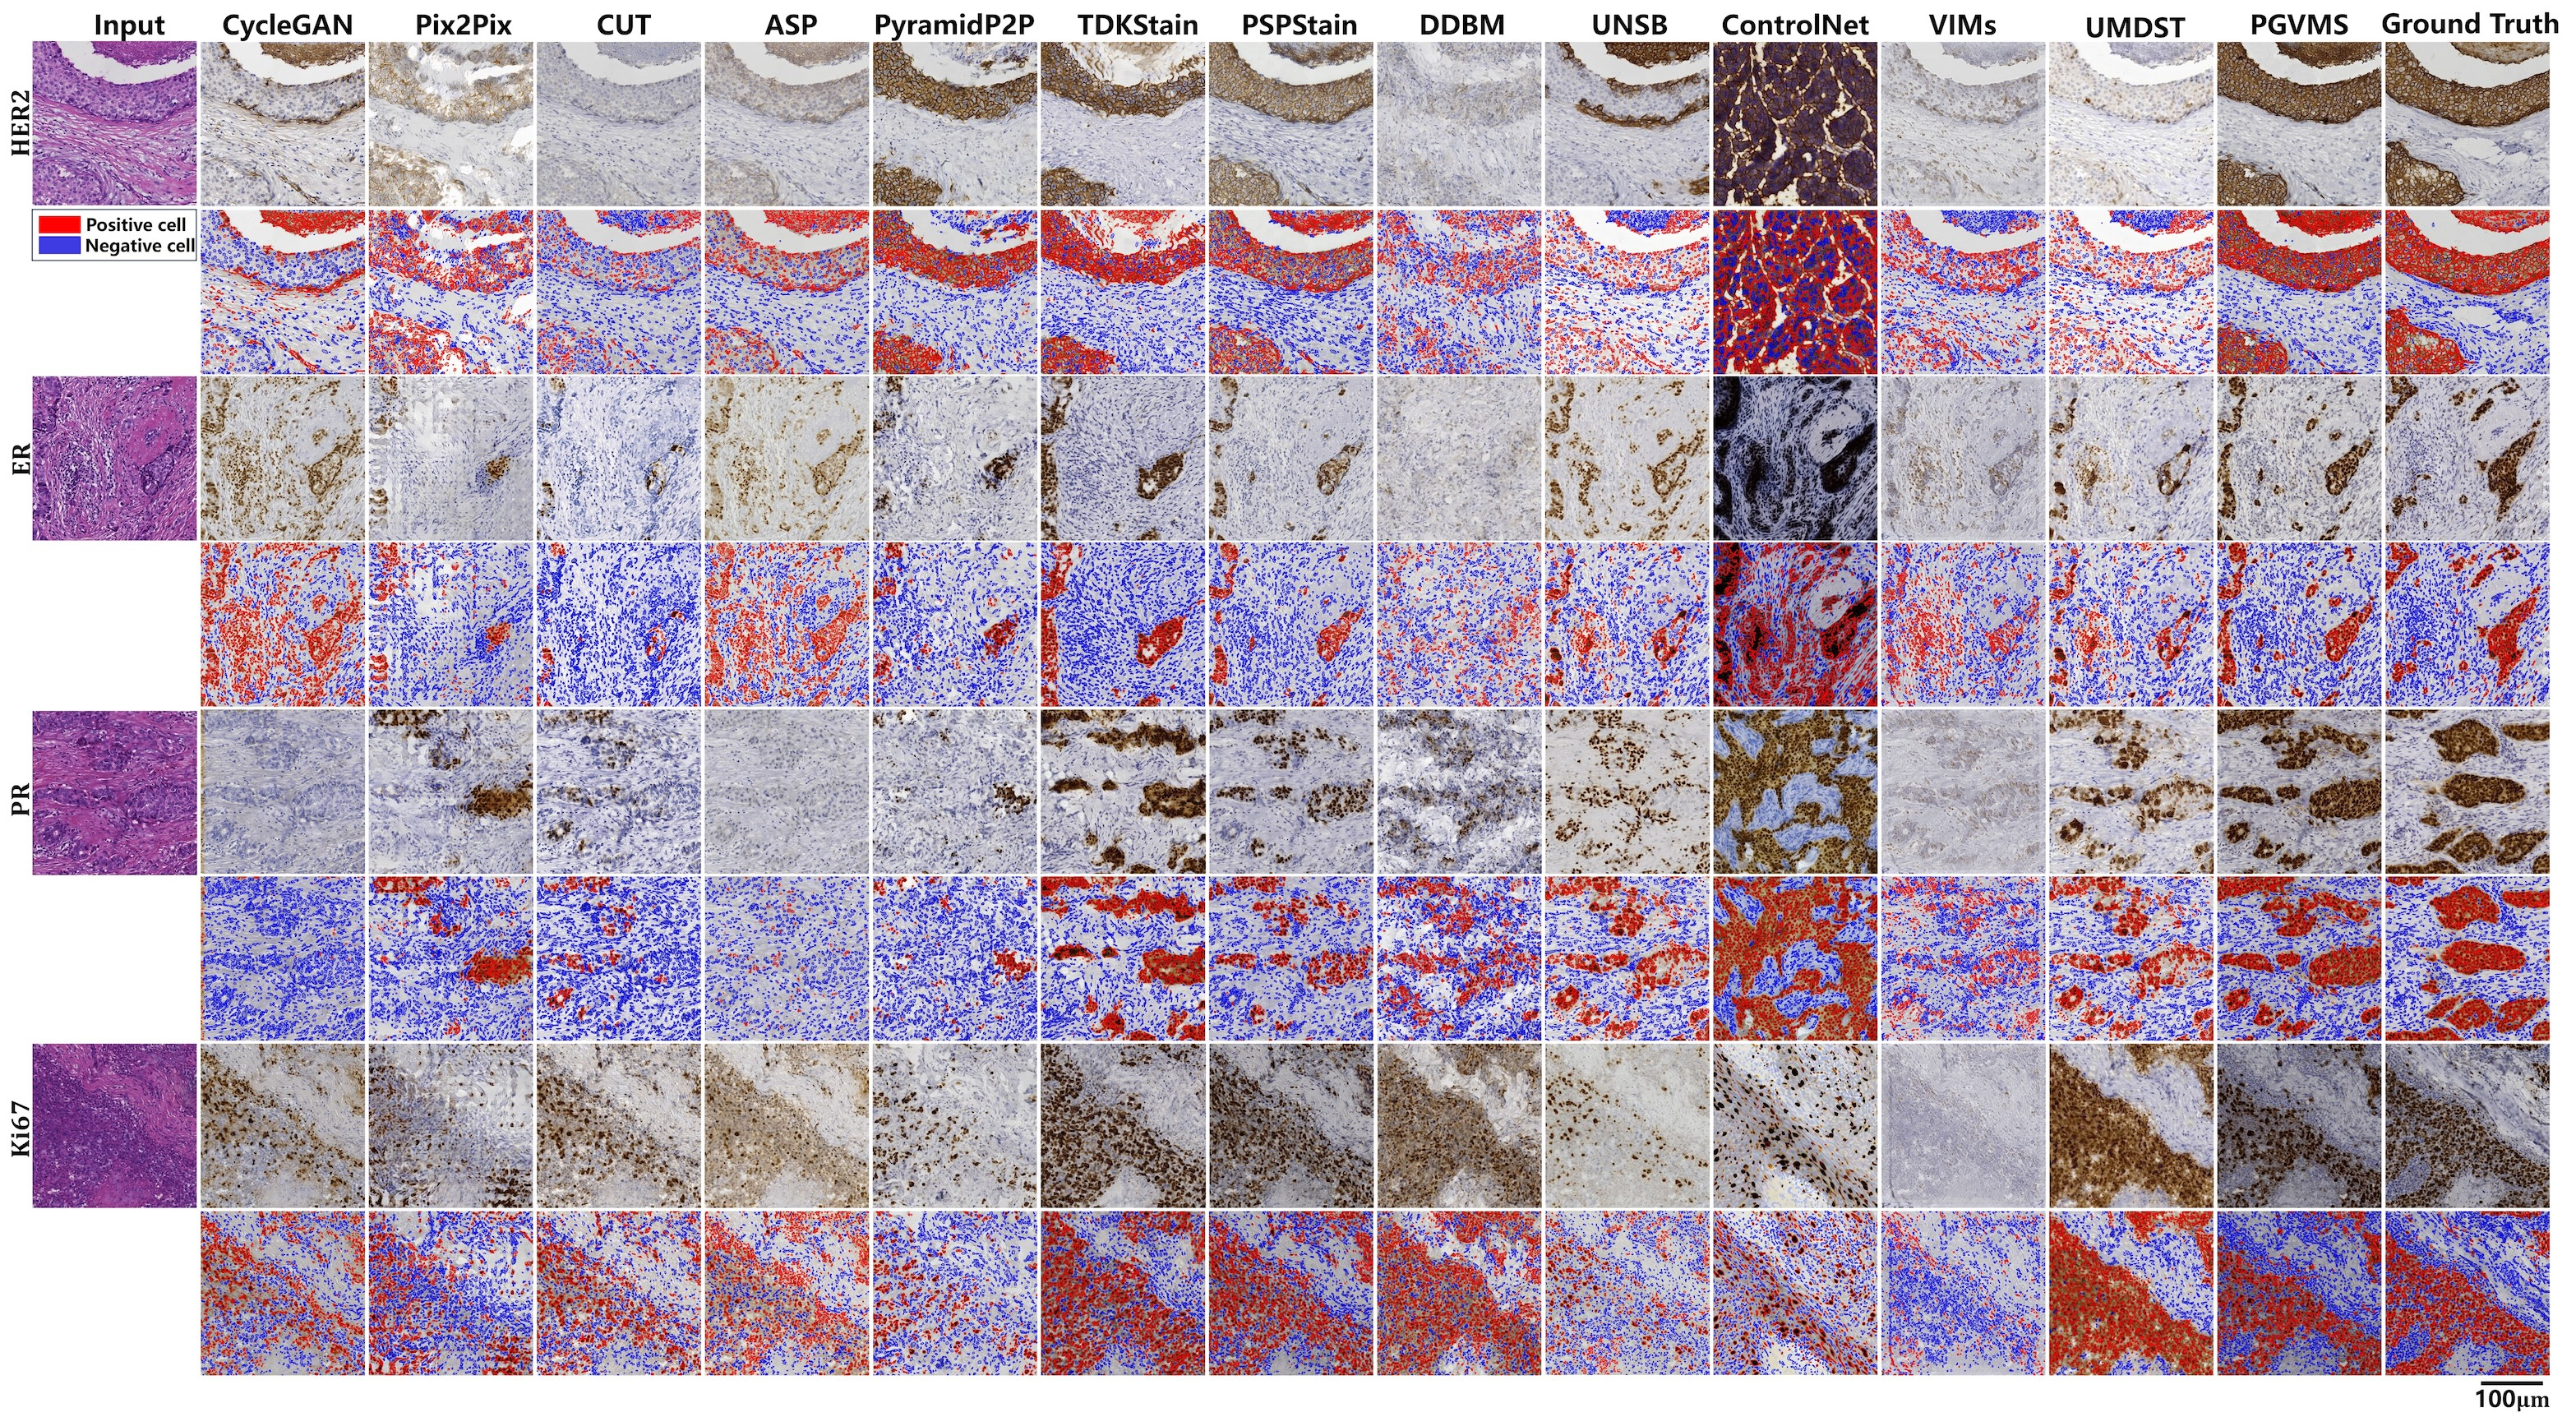
\includegraphics[width=\textwidth]{image/qin4.jpg}}
\caption{{Virtual IHC-stained image results of different methods on the MIST dataset. The first column is the H\&E-stained images. Columns 2 to 14 are the images virtually stained by different methods. The last column is the ground truth. The figure also demonstrates virtual IHC results alongside positive cell visualization from DeepLIIF.}}
\label{qualitative_1}
\end{figure*}



 % We compare the performance of our method to other SOTA methods quantitatively based on the MIST and IHC4BC datasets.
Empirical results (Tables \ref{tab:all_datasets} and \ref{tab:ihc4bc_results}) demonstrate our method's superiority in pathological correlation and perceptual consistency, 
% Empirical results (Tables \ref{tab:all_datasets} and \ref{tab:ihc4bc_results}) demonstrate our method's superiority, with significant improvements in pathological correlation and perceptual consistency, though conventional image quality metrics show limited improvements.
% Empirical results in Table. \ref{tab:all_datasets}  and Table. \ref{tab:ihc4bc_results} demonstrate the superiority of our method. Benchmarking reveals significant improvements in pathological correlation and perceptual consistency ,but not in image quality.
 % Initially, we employed PSNR and SSIM for initial image quality assessment, but their applicability is limited in this context. Differing staining principles between H\&E and IHC create imperfect pixel-level correspondence. Additionally, inherent structural disparities arise during dataset preparation. Therefore, these metrics serve only as reference values rather than definitive evaluation criteria.
% While we computed PSNR and SSIM as reference metrics, their validity is limited due to that the fundamental differences between H\&E and IHC staining inevitably cause structural variations in the resulting datasets. These metrics thus provide only references, not definitive evaluation criteria.
while conventional image quality metrics (PSNR and SSIM) show limited improvement due to inherent structural mismatches between the two staining modalities in the dataset\cite{liu2022bci}.
% while PSNR and SSIM for common image quality metrics, these pixel-based measures are  not ideal for stain transfer task due to inherent structural misalignment between two staining domains \cite{liu2022bci}.
As detailed in Section \ref{sec:discussion} with Table~\ref{tab:combined_psnrssim_results}, PSNR and SSIM provide only reference values rather than conclusive evaluation criteria.

%   The  We include PSNR and SSIM for quality metrics. 
%  However, PSNR and SSIM are not ideal for the stain transfer task due to the mismatched structure between the images of the two staining domains in the dataset\cite{liu2022bci}. 
%  Therefore, these metrics provide only reference values, rather than conclusive evaluation criteria.
% Our quantitative analysis of this phenomenon appears in the Section \ref{sec:ablation} with Table~\ref{tab:combined_psnrssim_results}.


 % Then we evaluate the pathological correlation (IOD and Pearson-R) in terms of the variation in total tumor expression levels and consistency of expression changes, respectively. For total tumor expression levels as shown in Tables \ref{tab:all_datasets} and \ref{tab:ihc4bc_results}, huge variation of IOD are obtained with the Pix2Pix, ASP and PyramidP2P; this demonstrating their weakness in preserving the tumor expression from the source images \cite{zhang2022mvfstain}. The other models show better tumor expression levels preserving in stain transfer, however our method achieved the best IOD. 
 We then evaluate pathological correlation (IOD and Pearson-R) in terms of variation in total protein expression levels and consistency of expression changes, respectively. For total protein expression levels, as shown in Tables \ref{tab:all_datasets} and \ref{tab:ihc4bc_results} pathology columns, huge variation in IOD is obtained with Pix2Pix, ASP, ControlNet and PyramidP2P, demonstrating their weakness in preserving protein expression from the source images \cite{zhang2022mvfstain}. While other models show better preservation of protein expression levels in stain transfer, our method achieves the best IOD. Furthermore, PGVMS achieves the highest Pearson-R score in both datasets, and this indicates that each generated image closely resembles the ground truth in terms of pathological correlation. These superior IOD and Pearson-R performance metrics of PGVMS can be attributed to the innovative components: PALS maintains protein expression levels matching ground truth, preserving pathological semantics, while PSSG integrates CONCH's semantic embeddings during stain transfer to ensure structural and biochemical fidelity.
 % And PGVMS achieves the highest Pearson-R score in the two datasets, indicating that each generated image closely resemble the ground truth in terms of pathological correlation. 
 % This advantage shows its excellent ability to maintain pathological consistency.
 
 % Finally,  We evaluate the visual perception (FID and DISTS), as shown in Tables \ref{tab:all_datasets} and \ref{tab:ihc4bc_results} perception column, our method achieved the lowest FID and DISTS metrics, demonstrating the most realistic stain transformation and tissue structure preservation for pathological diagnosis. In general, Tables \ref{tab:all_datasets} and \ref{tab:ihc4bc_results} shows our PGVMS solve the three challenges: (a) Inadequate semantic guidance for multi-staining ; b) Inconsistent distribution of immunochemistry staining; (c) Spatial misalignment of pathological semantics. 

 
 Finally, we evaluate the visual perception (FID and DISTS). As shown in Tables \ref{tab:all_datasets} and \ref{tab:ihc4bc_results} perception columns, our method achieved the lowest FID and DISTS metrics, demonstrating the most realistic stain transformation and tissue structure preservation for pathological diagnosis. This performance advantage stems from PCLS's design which enforces consistent feature embedding in latent space, thereby preserving key pathological features in synthesized protein margins and cellular atypia.
 % tumors with special accuracy in diagnostic-critical regions such as
 % In general, Tables \ref{tab:all_datasets} and \ref{tab:ihc4bc_results} show our PGVMS solves the three challenges: (a) Inadequate semantic guidance for multi-staining; (b) Inconsistent distribution of immunochemistry staining; (c) Spatial misalignment of pathological semantics.
 % focus on the weak paired characteristics between adjacent layer image pairs to neglect the adverse effects of tissue misalignment. Specifically, PSSG generator incorporates pathological semantic embeddings from CONCH during multi-stain transfer. PALS focuses on maintaining the tumor expression levels consistent with ground truth, enhancing the preservation of pathological semantic information. By incorporating PCLS, PGVMS preserves diagnostic pathological feature prototypes in generated tumors, achieving clinically significant fidelity.



 
%  For 
% Table. \ref{tab:all_datasets} shows that PGVMS achieves the lowest deviation of IOD and the highest Pearson-R score from the labels, indicating the highest pathological consistency. The higher PSNR and SSIM indicate higher image quality however not always in virtual staining. The lower awareness metric: FID and DISTS  demonstrates the effectiveness of our method. 





\begin{figure*}[t]
\centerline{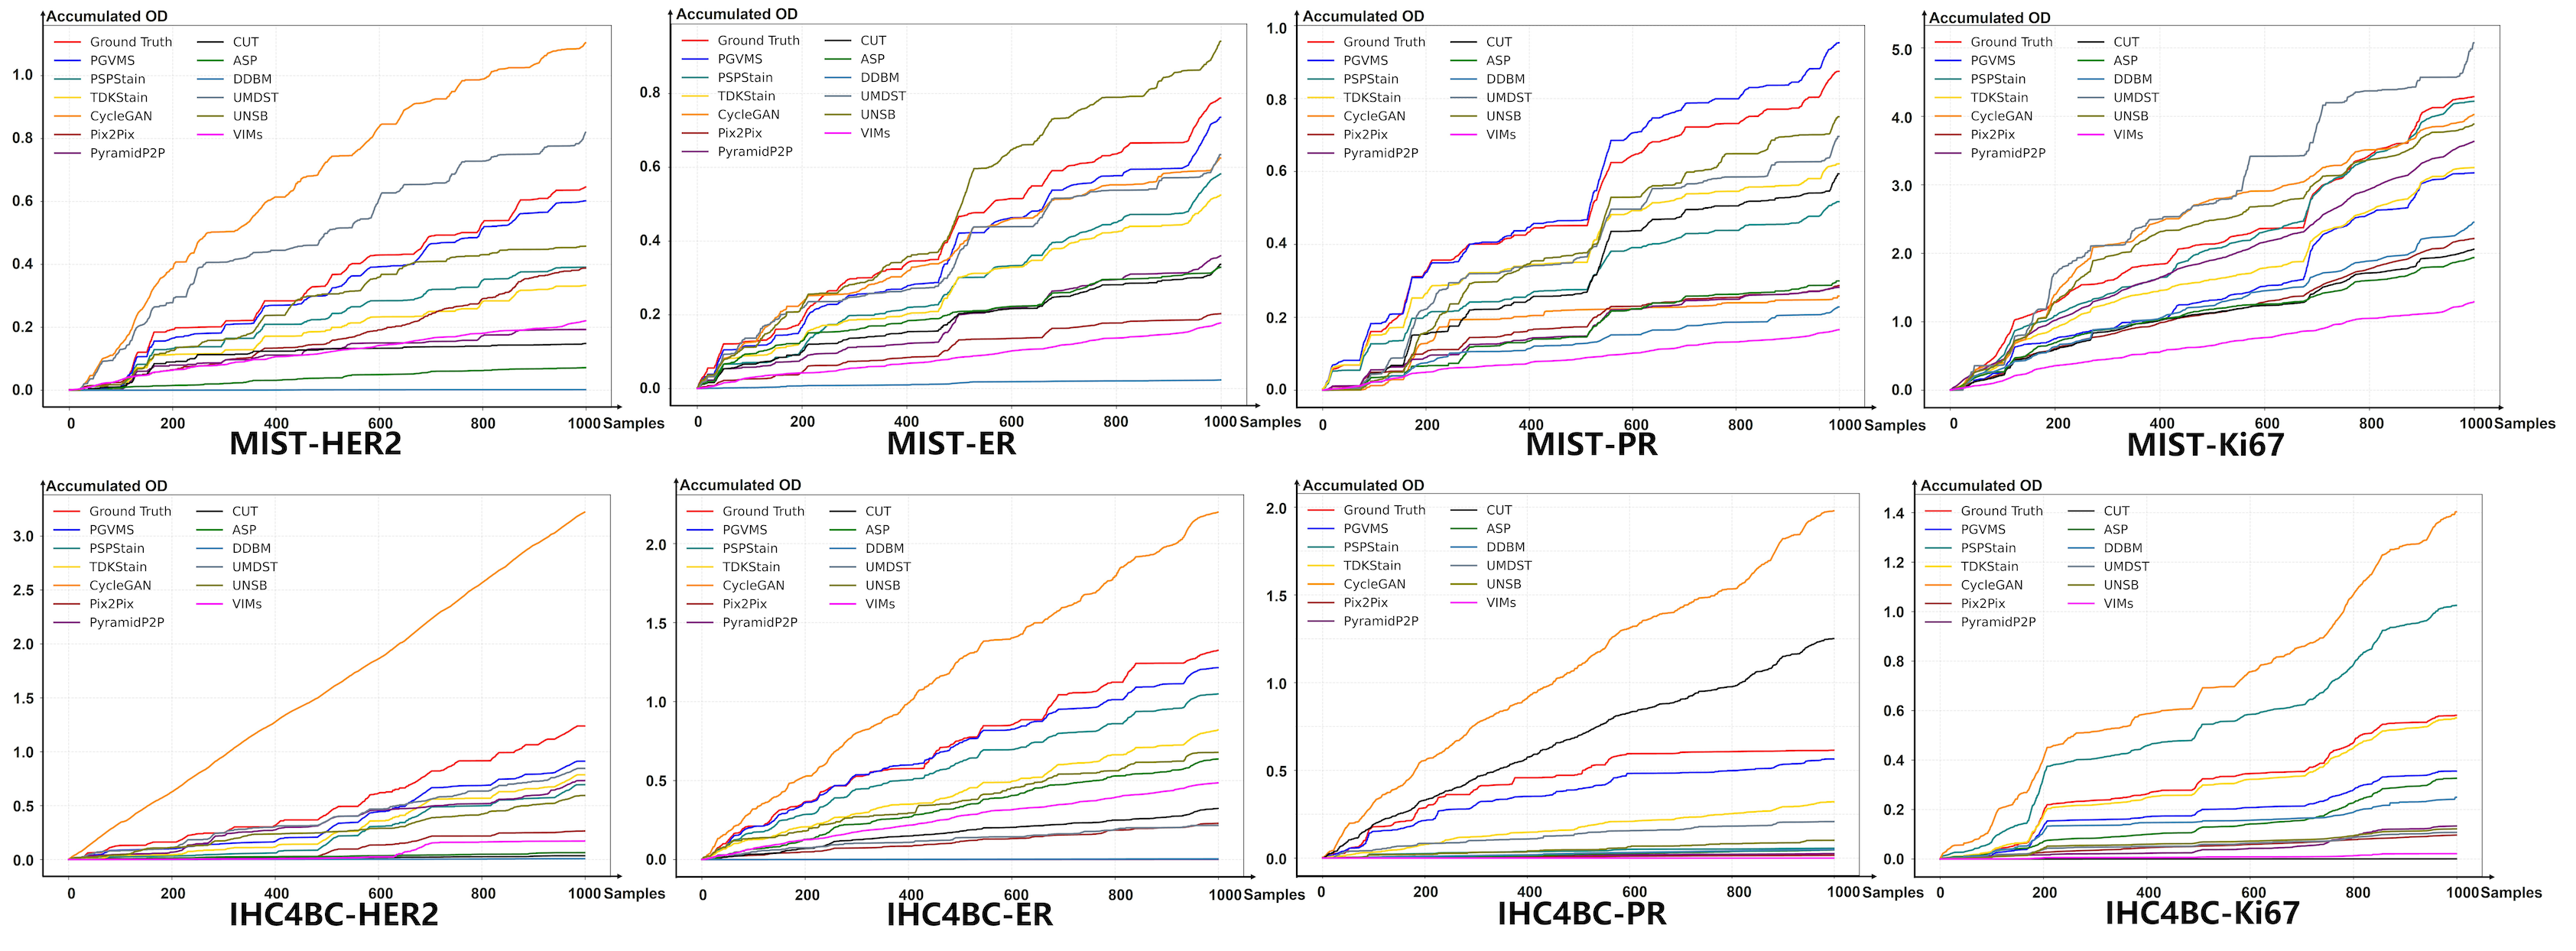
\includegraphics[width=\textwidth]{image/qin5.png}}
\caption{{Consistent with the protein progression tendency. The horizontal axis (abscissa) represents the sample index, while the vertical axis (ordinate) denotes the accumulated optical density (OD) value. The figure illustrates the accumulated OD curves of various virtual staining methods for IHC positive regions, comparing the virtual results with the reference IHC images on the MIST and IHC4BC datasets. The results of the ControlNet model are excluded because they deviate significantly from the ground truth.}}
\label{qualitative_2}
\end{figure*}

% More specifically, Conventional H\&E-to-IHC virtual staining methods, such as unsupervised approaches (CycleGAN, CUT) and semi-supervised methods (ASP), exhibit critical limitations in cross-modal semantic embedding transfer, evidenced by substantial IOD deviations ($\geq 2.5491 \times 10^{7}$ for HER2) and weak pathological correlations. While fully supervised methods like Pix2Pix and PyramidP2P improve structural metrics (SSIM $= 0.2200$ for ER), their reliance on pixel-level constraints exacerbates perceptual distortions (FID $= 80.49$ for PR) due to spatial misalignment. Addressing these challenges, the proposed \textbf{PGVMS} framework achieves breakthrough performance through three synergistic innovations that collectively enhance virtual staining quality. The \textbf{pathological semantics-guided generator backbone (PSSG)}, powered by the \textbf{CONCH} module, enables prompt-driven multi-stain adaptation, ensuring robust semantic embedding transfer across diverse staining tasks. Complementing this, the \textbf{protein-aware learning strategy (PALS)} employs \textbf{FOD} feature mapping to preserve molecular-level protein activation patterns, maintaining biological fidelity in the generated images. Finally, the \textbf{prototype-consistent learning strategy (PCLS)} enforces cross-image semantic topology consistency, mitigating spatial misalignment effects and improving inter-image coherence. Together, these innovations drive comprehensive performance improvements, as evidenced by state-of-the-art \textbf{R-values} ($0.8548$--$0.9126$), reduced \textbf{IOD} deviations ($-0.5193 \times 10^{7}$ for ER and $+0.7815 \times 10^{7}$ for PR), and optimized \textbf{DISTS} scores ($0.2299$--$0.2439$), surpassing conventional methods by $8.7\%$--$21.3\%$ across key metrics.

% Experimental validation highlights PGVMS’s multi-task superiority, including unified multi-stain adaptability (average PSNR $= 14.37$, outperforming task-specific models like ASP by $3.2\%$), unprecedented pathological correlation for Ki67 (mIOD $= +0.0074$), and spatial misalignment robustness (FID $\leq 36.58$, $17.4\%$ lower than alternatives). These advancements address core challenges in semantic embedding transfer, protein coherence preservation, and cross-slide topological consistency, establishing PGVMS as a transformative tool for computational pathology and diagnostic workflows.


\begin{figure*}[!htbp]
\centerline{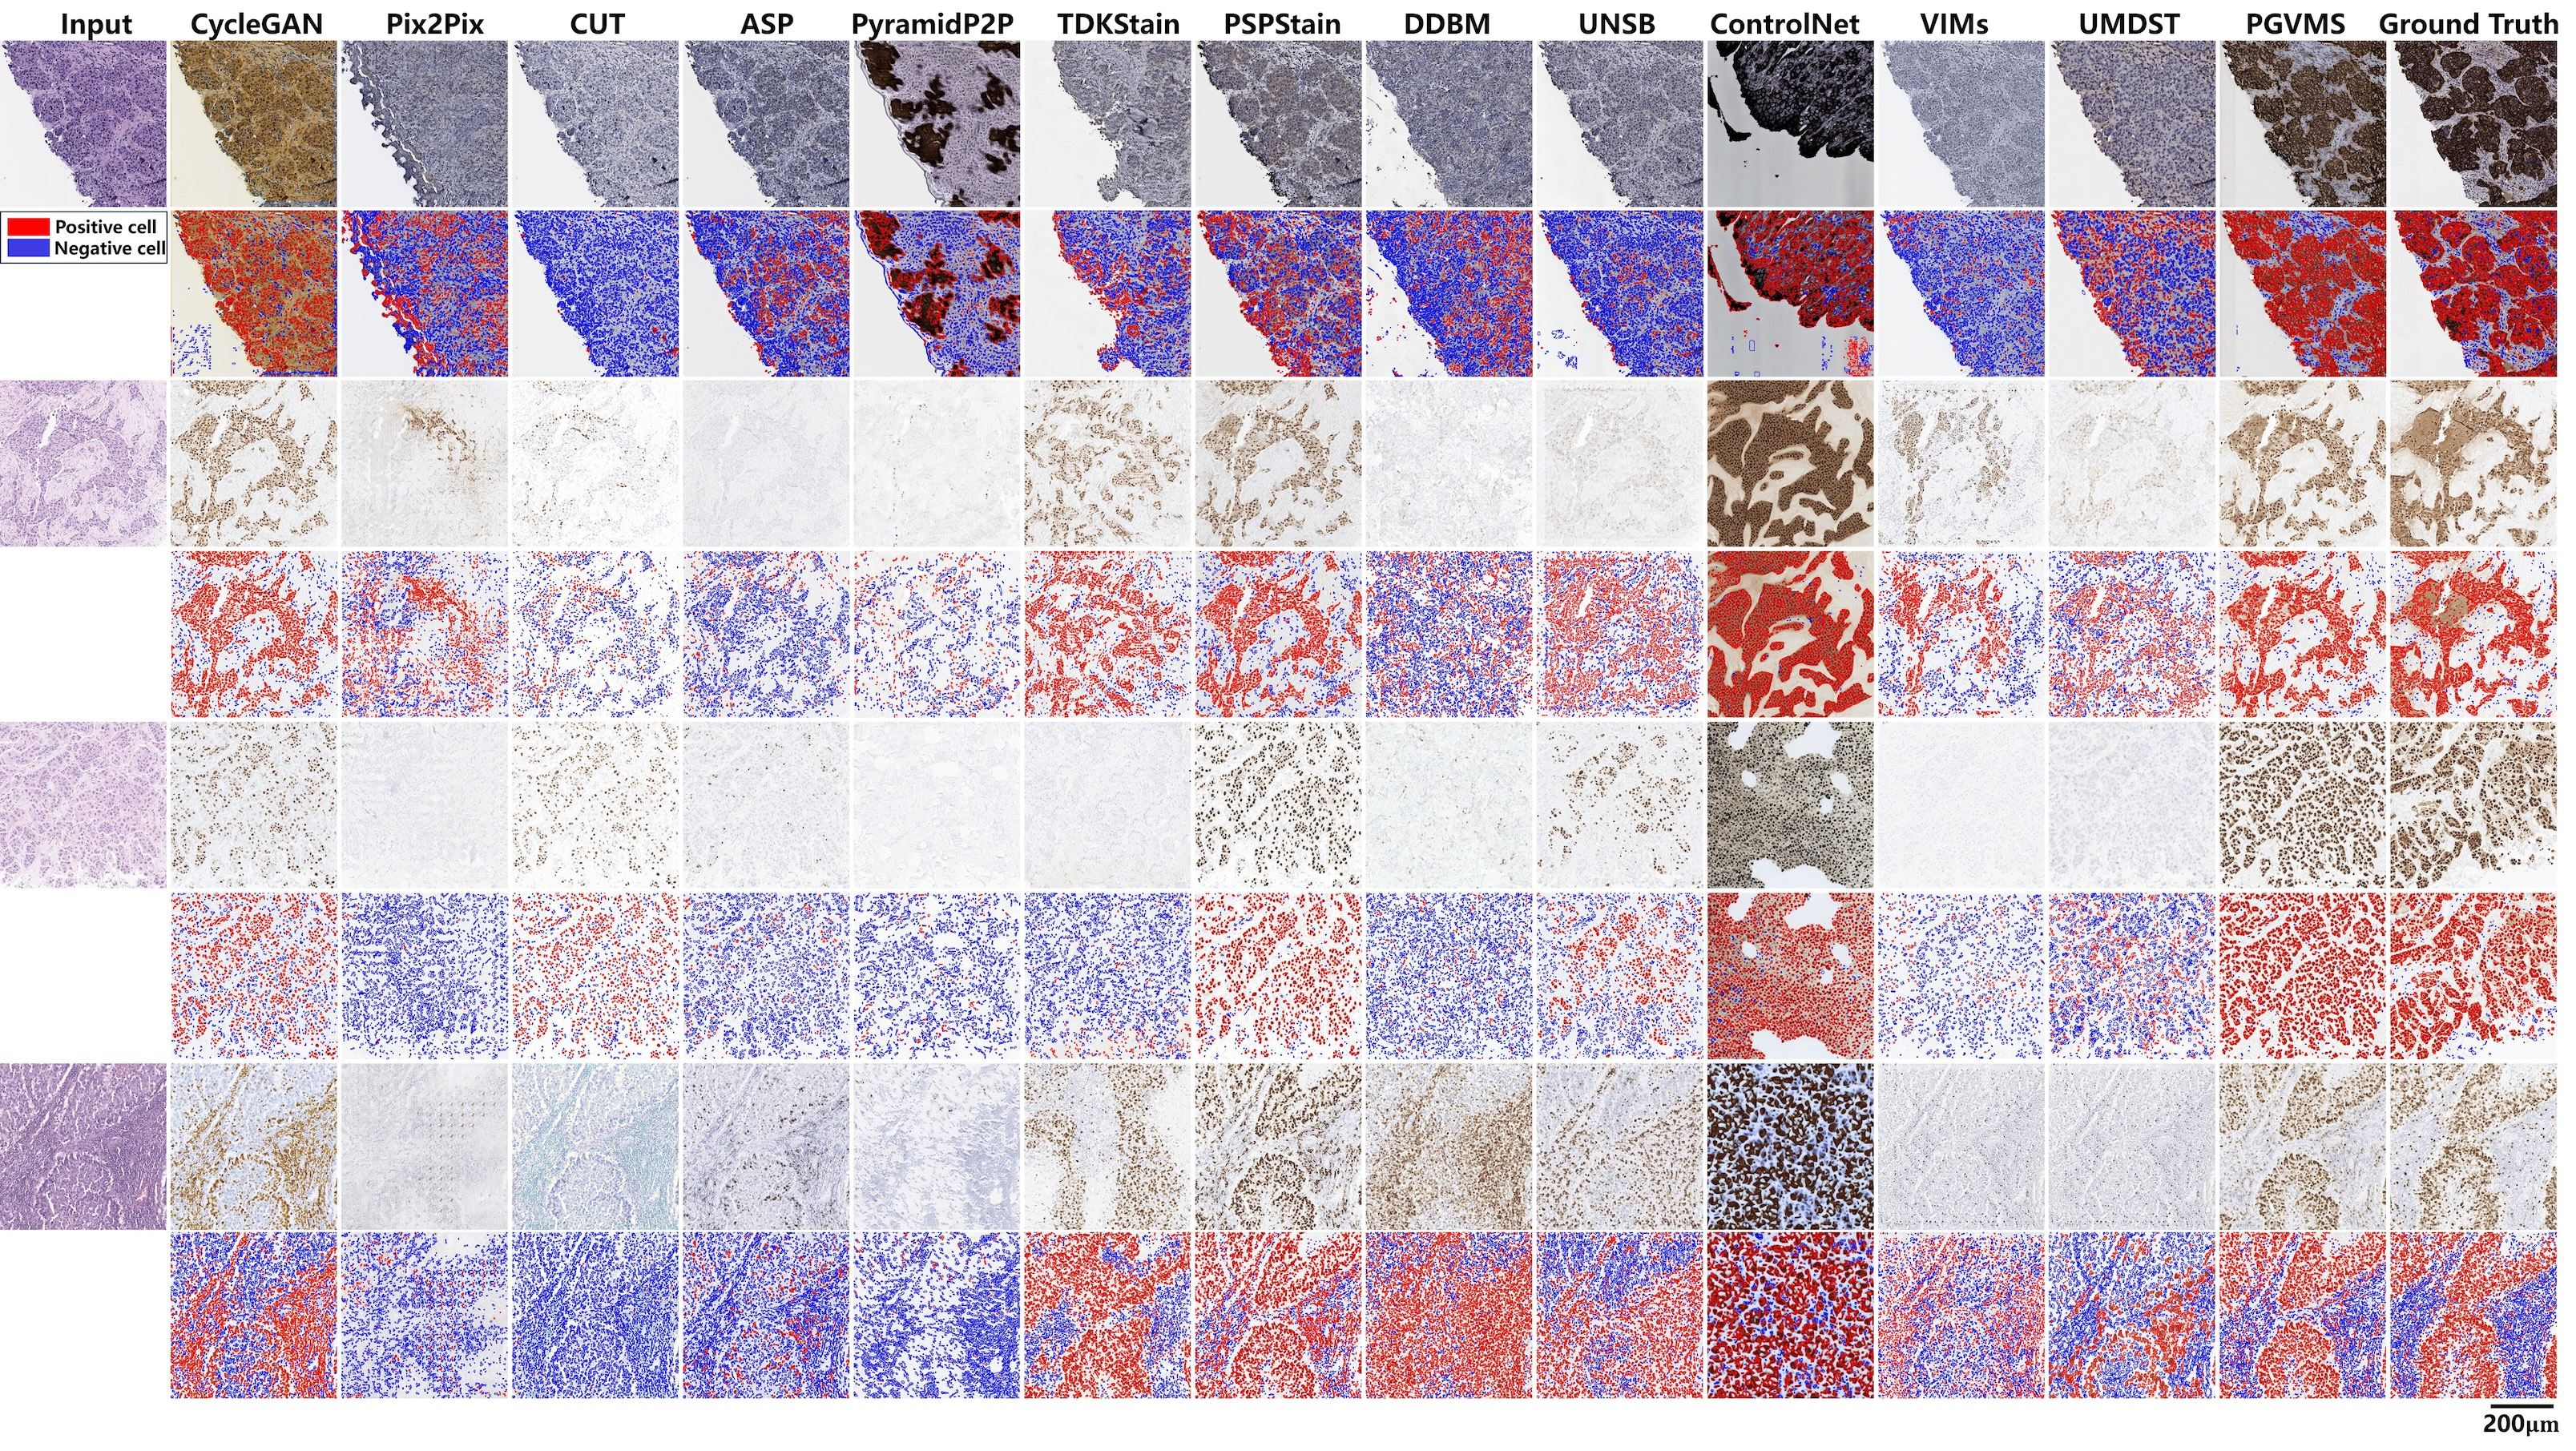
\includegraphics[width=\textwidth]{image/qin6.jpg}}
\caption{{Virtual IHC-stained image results of different methods on the IHC4BC dataset. The first column is the H\&E-stained images. Columns 2 to 14 are the images virtually stained by different methods. The last column is the ground truth. The figure also demonstrates virtual IHC results alongside positive cell visualization from DeepLIIF.}}
\label{qualitative_ihc4bc}
\end{figure*}



% Specifically, the blurry IHC images with more averaged pixel value may cause them to be increased within spatial misalignment~\cite{zhu2023breast}.The results are displayed in Table II. Compared with the comparison methods, our method
%  achieves the best results in terms of the SSIM, PSNR and FID metrics. This fully demonstrates the effectiveness of our method for virtual staining.
\subsubsection{Qualitative Assessment} To further explore the visual differences in the virtual staining, we present the results of our method and other competing methods on MIST dataset in Fig. \ref{qualitative_1} and IHC4BC dataset in Fig. \ref{qualitative_ihc4bc}. {DeepLIIF \cite{ghahremani2022deep} was used to highlight positive cells (red) and negative cells (blue).} Compared with others, the virtual IHC images generated by our method are most similar with the real IHC images.

Fig. \ref{qualitative_1} and Fig. \ref{qualitative_ihc4bc} reveals that existing methods like CycleGAN, Pix2Pix, and CUT produce IHC images with inaccurate pathological characteristics due to insufficient supervisory information. Moreover, ASP and PyramidP2P contain insufficient pathological characteristics due to the patch-level loss between virtual IHC images and weakly paired ground truth. {ControlNet often produces hallucinations due to the lack of sufficient pathological constraints. VIMs and UMDST, as one-to-many methods, lack the precision to identify protein overexpression regions accurately.}
In contrast, both TDKStain and PSPStain detect the protein expression amount, thus they maintain strong pathological relevance with real IHC images.  However, TDKStain often produces wrong tumor shapes and distributions (Fig. \ref{tdkstain_unpair}), as it fails to accurately capture cellular localization and may introduce spurious cellular artifacts. Meanwhile, PSPStain preserves the tissue structure in H\&E-stained images through semantic preservation. Notably, virtual IHC images generated by PGVMS exhibit closer similarity to referenced adjacent-layer IHC images by learning pathological semantics—particularly in highlighting small high-protein expression areas missed by other methods.
% Fig. \ref{qualitative_1} reveals that existing method like CycleGAN, Pix2Pix and CUT produce IHC images with inaccurate pathological characteristics due to insufficient supervisory information. ASP and PyramidP2P contain insufficient pathological characteristics due to the patch-level loss between virtual IHC images and weakly paired ground truth. In another hand, both TDKStain and PSPStain  detect the protein expression amount, so they have strong pathological relevance with real IHC image. But TDKStain always produce wrong shape and distribution of tumor, this is because TDKStain can not overlook tissue misalignment and deformation between weakly paired images. And PSPStain can preserve the tissue structure in  H\&E stained images with semantic preserving. But virtual IHC images generated by  
%  PGVMS are more similar to the referenced adjacent layer IHC images due to learning the pathological semantics, especially highlight the small tumor area that other method missed.
\subsubsection{Protein Expression Analysis}
Typically, pathologists pay more attention to the protein expression level of IHC staining when analyzing IHC images \cite{li2025biomedical}. Therefore, the accuracy of virtual IHC images can be effectively evaluated by studying the correlation between the protein expression level in virtual IHC images and those in real IHC images from adjacent layers.

% We determine the corresponding tumor expression level of the IHC patches. 
For each IHC patch, the H channel and the DAB channel can be separated using deconvolution. In the DAB channel, we calculate the tumor expression level for each patch and then accumulate the expression levels across all patches \cite{chen2024pathological}, as shown in the line chart (Fig. \ref{qualitative_2}). The red line in the chart represents the cumulative curve of positive protein expression levels for the reference. Notably, CycleGAN (orange) exhibits substantial deviation from the reference (red) trajectory, indicating poor pathological concordance. {The results of the ControlNet model are excluded because they deviate significantly from the ground truth.} PSPStain (cyan) and TDKStain (yellow) exhibit good consistency. However, our PGVMS (blue) demonstrates the closest approximation to the reference profile across three stain types, visually confirming its superior pathological consistency with authentic IHC results.




{
\subsubsection{Downstream Classification Experiments}
To evaluate the diagnostic value of virtual staining, we assessed the impact of generated IHC images on downstream biomarker classification (Table~\ref{tab:combined_classification_full_2}) using a ViT-B/32 backbone classifier. Separate models were trained for each biomarker—HER2, ER, PR, and Ki67—on the MIST and IHC4BC datasets to measure how well pathological information was preserved.
}
\begin{table}[ht]
\centering
\caption{{Classification accuracy (\%) of virtual staining results on MIST and IHC4BC datasets. HER2: 4-class (0, 1+, 2+, 3+); ER, PR, Ki67: binary (negative/positive). Models are grouped into one-to-one and one-to-many categories.}}
\resizebox{\columnwidth}{!}{
\begin{tabular}{l|cccc|cccc}
\Xhline{1.3pt}
\multirow{2}{*}{Method} & \multicolumn{4}{c|}{MIST} & \multicolumn{4}{c}{IHC4BC} \\
\cline{2-9}
 & HER2 & ER & PR & Ki67 & HER2 & ER & PR & Ki67 \\
\hline
% ---------------- One-to-one ----------------
CycleGAN    & 0.453     & 0.570     & 0.534    & 0.767     & 0.495     & 0.600     & 0.479     & 0.771     \\
Pix2Pix     & 0.490 & 0.671 & 0.671 & \underline{0.847} & 0.422 & 0.595 & 0.666 & 0.613 \\
CUT         & 0.457     & 0.610     & 0.664     & 0.807     & 0.258     & 0.573     & 0.492     & 0.565     \\
ASP         & 0.378 & 0.623 & 0.637 & 0.759 & 0.256 & 0.547 & 0.559 & 0.799 \\
PyramidP2P  & 0.587 & 0.695 & 0.705 & 0.842 & 0.505 & 0.497 & 0.640 & 0.686 \\
TDKStain    & \underline{0.642} & \textbf{0.798} & \underline{0.812} & \textbf{0.857} & \textbf{0.541} & \textbf{0.667} & 0.571 & \underline{0.834} \\
PSPStain    & \textbf{0.647} & 0.763 & 0.768 & 0.844 & 0.474 & 0.596 & \textbf{0.750} & 0.763 \\
DDBM        & 0.420 & 0.584 & 0.577 & 0.634 & 0.449 & 0.534 & 0.629 & 0.754 \\
UNSB        & 0.450 & 0.642 & 0.611 & 0.802 & 0.397 & 0.563 & 0.626 & 0.782 \\
\Xhline{0.8pt}
% ---------------- One-to-many ----------------
\rowcolor{gray!10}
ControlNet  & 0.329 & 0.673 & 0.537 & 0.844 & 0.470 & 0.558 & 0.352 & 0.599 \\
\rowcolor{gray!10}
VIMs        & 0.309 & 0.652 & 0.561 & 0.795 & 0.326 & 0.626 & 0.657 & 0.578 \\
\rowcolor{gray!10}
UMDST       & 0.419 & 0.572 & 0.655 & 0.843 & 0.251 & 0.462 & 0.640 & 0.687 \\
\rowcolor{gray!10}
PGVMS       & 0.617 & \underline{0.772} & \textbf{0.818} & 0.740 & \underline{0.535} & \underline{0.627} & \underline{0.678} & \textbf{0.865} \\
\Xhline{1.3pt}
\end{tabular}
}
\label{tab:combined_classification_full_2}
\end{table}

{
HER2 was treated as a four-class problem (0, 1+, 2+, 3+) based on cumulative OD thresholds of 500, 2000, and 5000. ER and PR were binarized at 1000, and Ki67 at 2000, following established cutoffs \cite{varghese2014ihc}. All automated labels were subsequently reviewed by board-certified pathologists.
}

\begin{figure}[!htbp]
\centerline{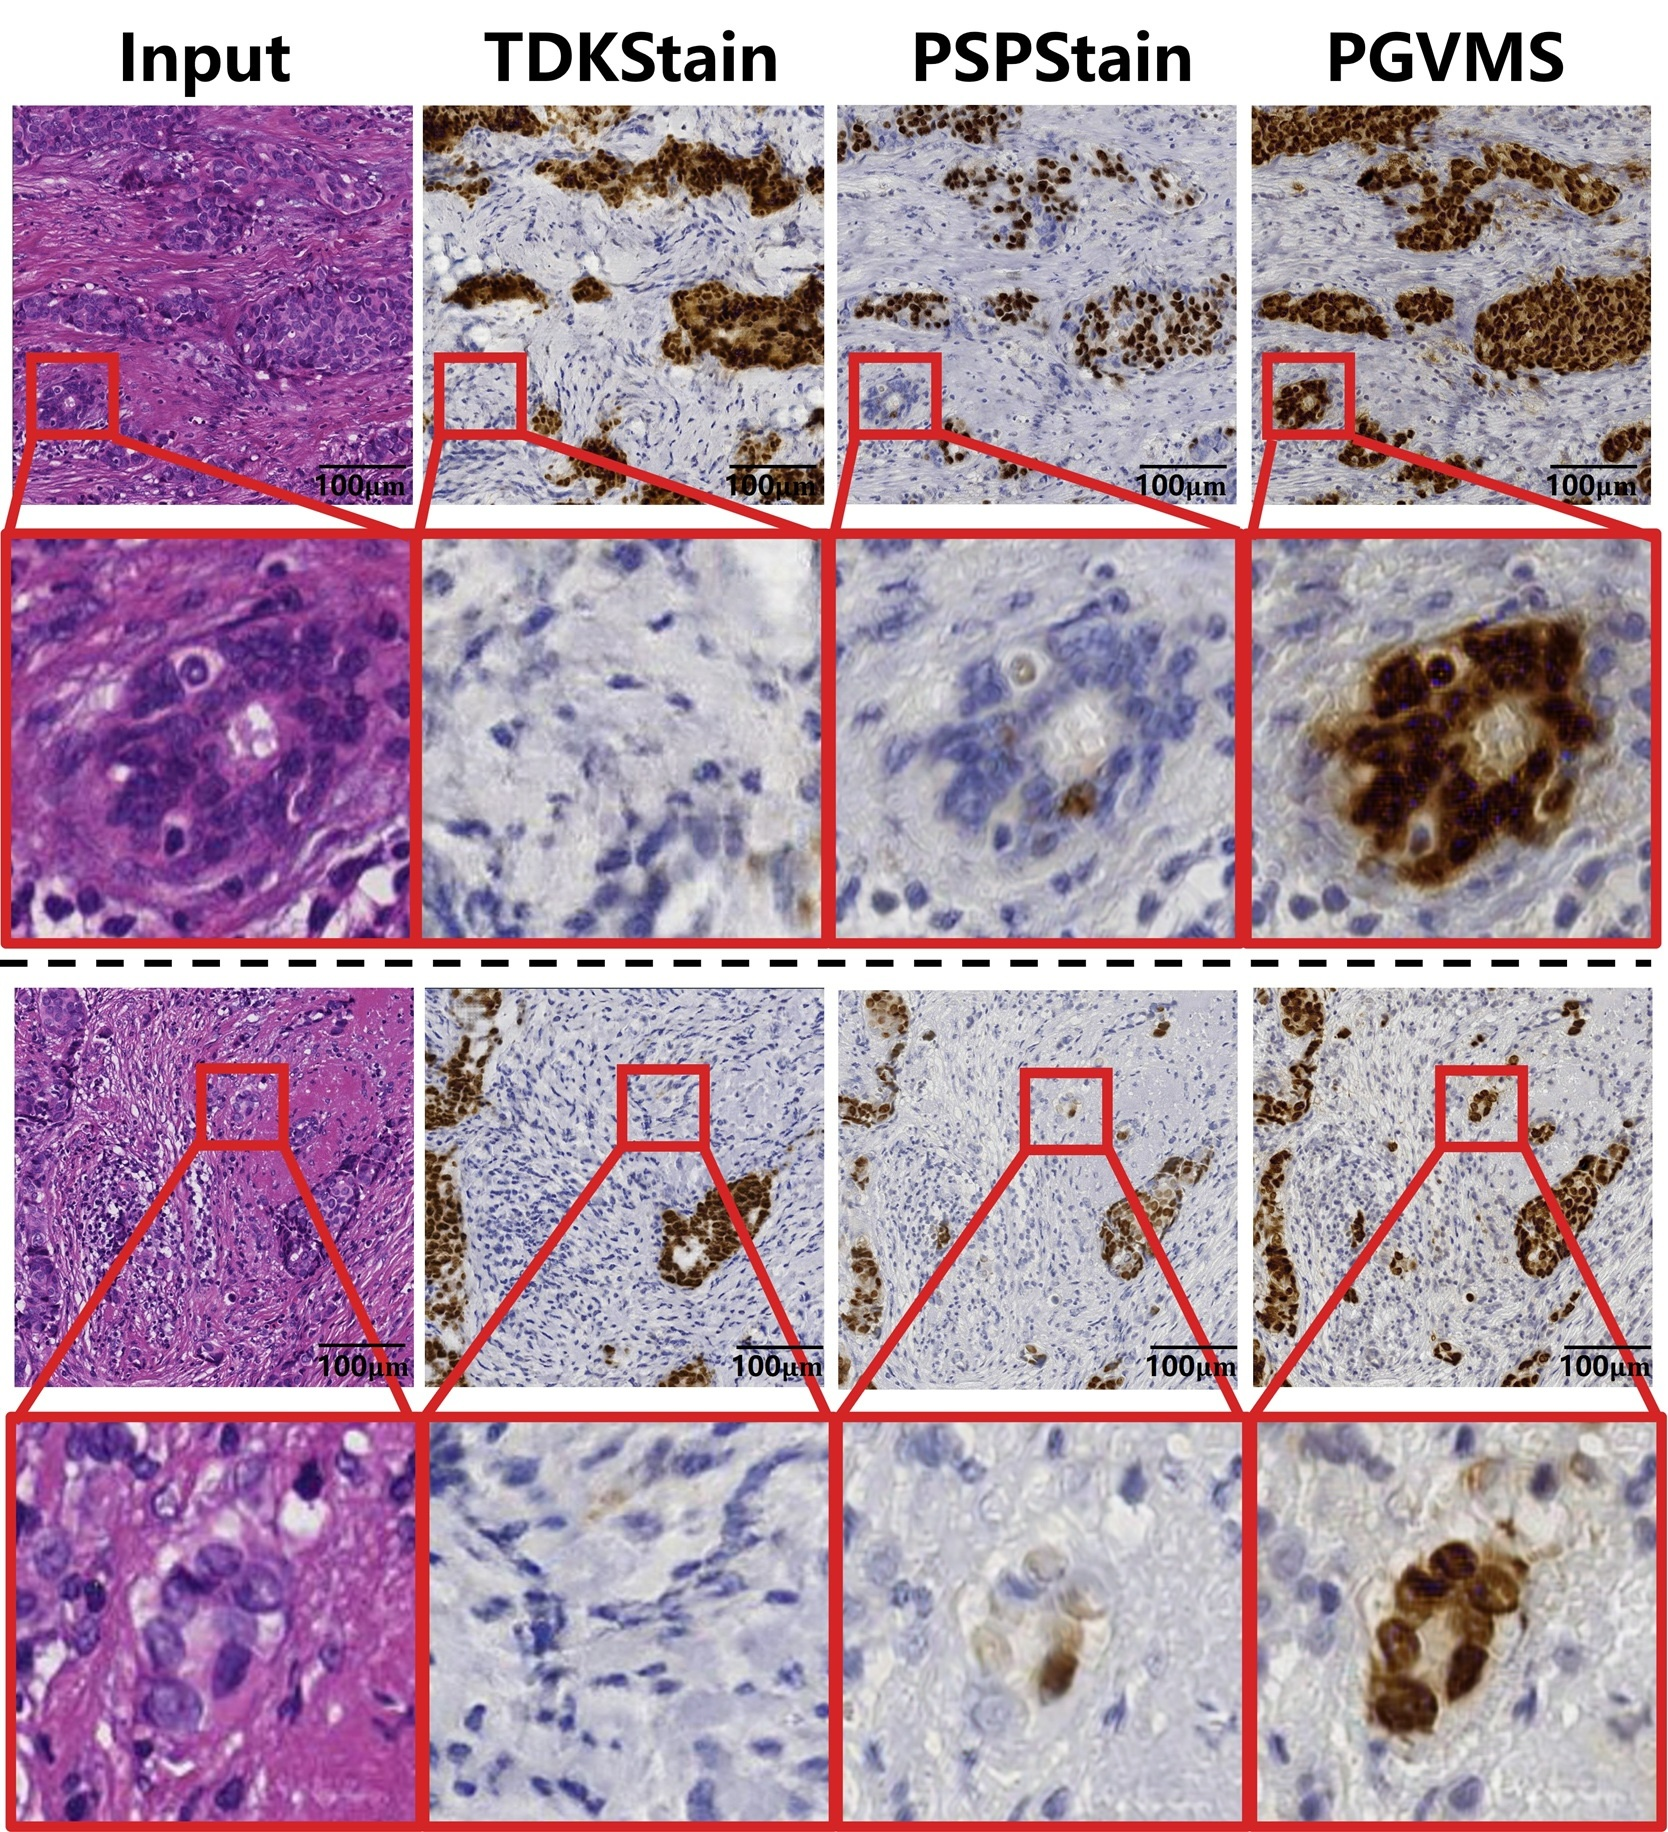
\includegraphics[width=\columnwidth]{image/qin7.jpg}}
\caption{{Visual comparison illustrating the severe cell spatial misalignment issue in TDKStain results, where virtual staining causes substantial cell displacement relative to the input H\&E image. In contrast, our PGVMS method preserves accurate cell spatial localization.}}
\label{tdkstain_unpair}
\end{figure}


{
As shown in Table~\ref{tab:combined_classification_full_2}, TDKStain achieves the highest classification accuracy, followed by PGVMS and PSPStain. However, TDKStain shows severe cell localization errors, with notable misalignment between the generated IHC and input H\&E images (Figure~\ref{tdkstain_unpair}), significantly limiting its clinical usability.
}
% This can be quantitatively evaluated using the structural Pearson coefficient, which converts the input and output images to grayscale and computes the Pearson correlation along the spatial dimension. And as shown in Table~\ref{tab:pearson_structure}, TDKStain’s structural similarity is particularly low, ranging from 0.07 to 0.2, whereas most other methods—including ours—demonstrate good cell localization with values around 0.8, with CycleGAN performing the best.







\subsubsection{Feature-Level Metric Based on Pathological Foundation Model CONCH}
{
To assess the feature-level alignment of virtual IHC images with clinical pathology, we encode both the generated and ground-truth IHC images using the pre-trained image encoder of CONCH, producing a 512-dimensional feature vector for each image. The CONCH-FID is then calculated as the Fréchet distance between the distributions of these embeddings, capturing how well the generated images preserve high-level, pathology-specific semantic features. As shown in Table~\ref{tab:combined_fid_conch_5}, our PGVMS method ranks second on the MIST dataset, first on the IHC4BC dataset, and achieves the best overall performance across datasets. In comparison, PSPStain ranks second overall, while ASP comes third. These results highlight PGVMS’s superior ability to generate virtual IHC images that closely replicate the structural and semantic characteristics of authentic clinical slides.
}
\begin{table*}[!htbp]
\centering
\caption{{Feature-level FID between virtual IHC and ground-truth IHC computed using the pathology foundation model CONCH. Lower values indicate better alignment. The best and second-best results are highlighted in \textbf{bold} and \underline{underlined}, respectively.}}
\label{tab:combined_fid_conch_5}
\setlength{\tabcolsep}{4pt}
\renewcommand{\arraystretch}{1.15}
\resizebox{\textwidth}{!}{
\begin{tabular}{l|l|cccc|c||cccc|c}
\Xhline{1.3pt}
Type & Method 
& \multicolumn{5}{c||}{\textbf{MIST}} 
& \multicolumn{5}{c}{\textbf{IHC4BC}} \\
\cline{3-12}
& & HER2 & ER & PR & Ki67 & Mean 
& HER2 & ER & PR & Ki67 & Mean \\
\hline
\multirow{9}{*}{One-to-one}
& CycleGAN   & 102.1581 & 52.9350 & 125.7399 & 48.0381 & 82.2178 & 218.4938 & 44.1311 & 81.4923 & 49.0361 & 98.2884 \\
& Pix2Pix    & 95.9983 & 189.5522 & 182.9658 & 216.5276 & 171.2610 & 153.2364 & 105.1925 & 95.7887 & 128.3961 & 120.6534 \\
& CUT        & 62.6960 & 39.4071 & \underline{32.4882} & 35.4223 & 42.5034 & 80.8654 & 32.3410 & 39.4285 & 247.6296 & 100.0661 \\
& ASP        & \underline{39.9833} & 52.4421 & 38.3425 & 43.7905 & 43.6396 & 76.8791 & \underline{25.4769} & \underline{31.9873} & \textbf{20.9709} & \underline{38.8285} \\
& Pyramid    & 151.2503 & 153.7980 & 145.9719 & 172.3845 & 155.8512 & 237.9637 & 172.1971 & 162.0819 & 106.7118 & 169.7386 \\
& TDKStain   & 85.3784 & 73.2279 & 98.2533 & 143.9924 & 100.2130 & \underline{49.5412} & 61.5834 & 75.3190 & 52.3977 & 59.7103 \\
& PSPStain   & \textbf{34.7499} & \textbf{30.8958} & 32.7645 & \textbf{26.2759} & \textbf{31.1715} & \textbf{47.1362} & 35.2759 & 48.1594 & 36.9802 & 41.8879 \\
& DDBM       & 291.1494 & 281.9772 & 244.6667 & 215.1843 & 258.2444 & 326.7613 & 256.5512 & 258.2804 & 182.5962 & 256.0473 \\
& UNSB       & 61.9792 & 38.1701 & 49.4495 & 36.9417 & 46.6351 & 64.6003 & 69.6588 & 37.2139 & 48.7528 & 55.0565 \\
\hline
\rowcolor{gray!10}

& ControlNet & 283.2979 & 253.5201 & 317.4814 & 490.4310 & 336.1826 & 322.7134 & 432.5187 & 455.0586 & 434.0198 & 411.0776 \\
\rowcolor{gray!10}
& VIMs       & 353.5241 & 240.2728 & 234.2091 & 233.9704 & 265.4941 & 192.7621 & 140.0983 & 177.3091 & 166.0101 & 169.0449 \\
\rowcolor{gray!10}
& UMDST      & 154.3398 & 168.4891 & 147.7141 & 254.2693 & 181.2031 & 98.5943 & 116.0732 & 100.4608 & 184.7146 & 124.9607 \\

\rowcolor{gray!10}
\multirow{-4}{*}{One-to-many}& PGVMS 
& 55.1115 & \underline{31.0460} & \textbf{23.5529} & \underline{29.5545} & \underline{34.8162} 
& 61.7747 & \textbf{24.5485} & \textbf{30.8413} & \underline{21.8956} & \textbf{34.7650} \\
\Xhline{1.3pt}
\end{tabular}
}
\end{table*}



\subsubsection{Pathologist-Based Image Quality Evaluation}
{
To assess the clinical feasibility of our virtual staining results, we invited experienced pathologists to conduct a subjective quality evaluation. Specifically, for each dataset (MIST and IHC4BC), 50 randomly selected patches per stain were scored on a 1–5 scale based on three criteria: cellular localization, staining heterogeneity, and staining intensity. Scores of 3 and above indicate acceptable quality, while scores below 3 are considered unsatisfactory.
}
{
As illustrated in Fig.~\ref{qualitative_path_MIST} and Fig.~\ref{qualitative_path_IHC4BC}, the virtual IHC-stained images achieve consistently high quality across all criteria, with mean scores exceeding 3.0 and often approaching 4.0 or higher. On the MIST dataset, ER and PR stains receive the highest scores in both localization and intensity, suggesting that the model effectively preserves nuclear and cytoplasmic structures. On the IHC4BC dataset, HER2 and Ki67 exhibit stable performance across all aspects, demonstrating good generalization to cross-domain and inter-patient variations.
}
{
Overall, these results confirm that our method generates visually convincing and histologically consistent virtual IHC images, which are well accepted by pathologists and hold strong potential for clinical application.
}

\begin{figure}[!htbp]
\centerline{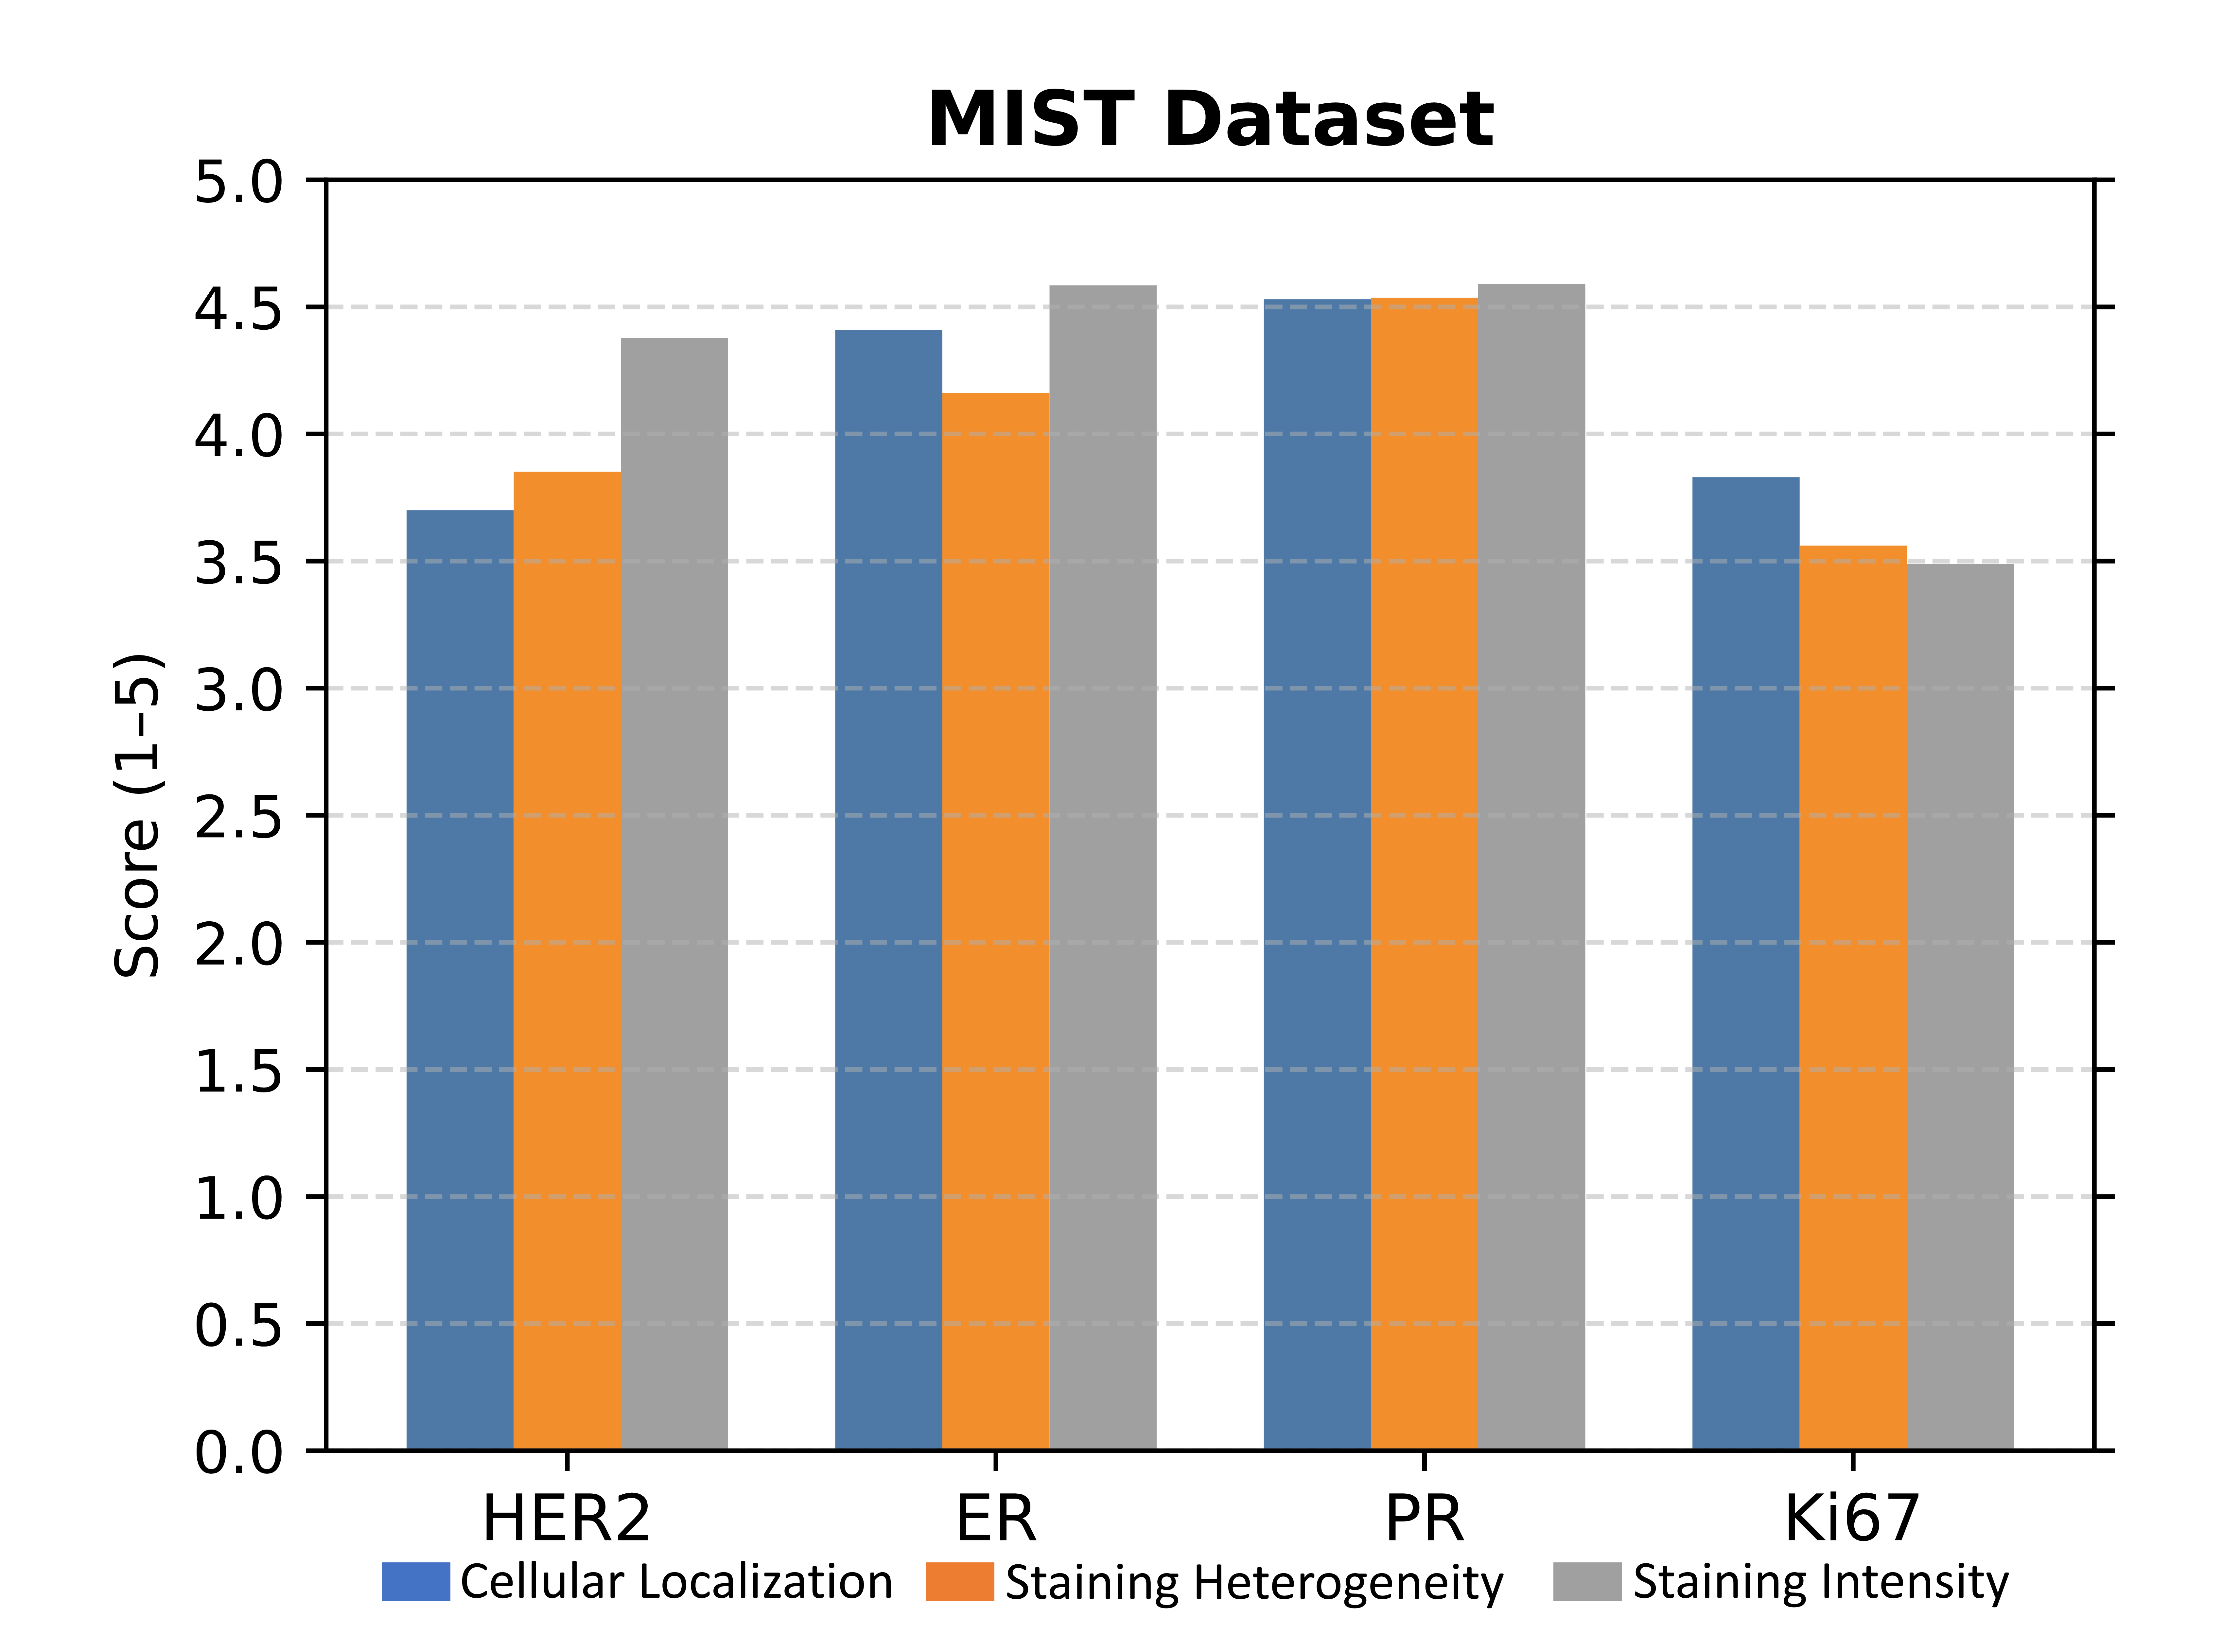
\includegraphics[width=\columnwidth]{image/qin8.png}}
\caption{{Pathologist evaluation of virtual IHC-stained images on the MIST datasets across three criteria: cellular localization, staining heterogeneity, and staining intensity.}}
\label{qualitative_path_MIST}
\end{figure}

\begin{figure}[!htbp]
\centerline{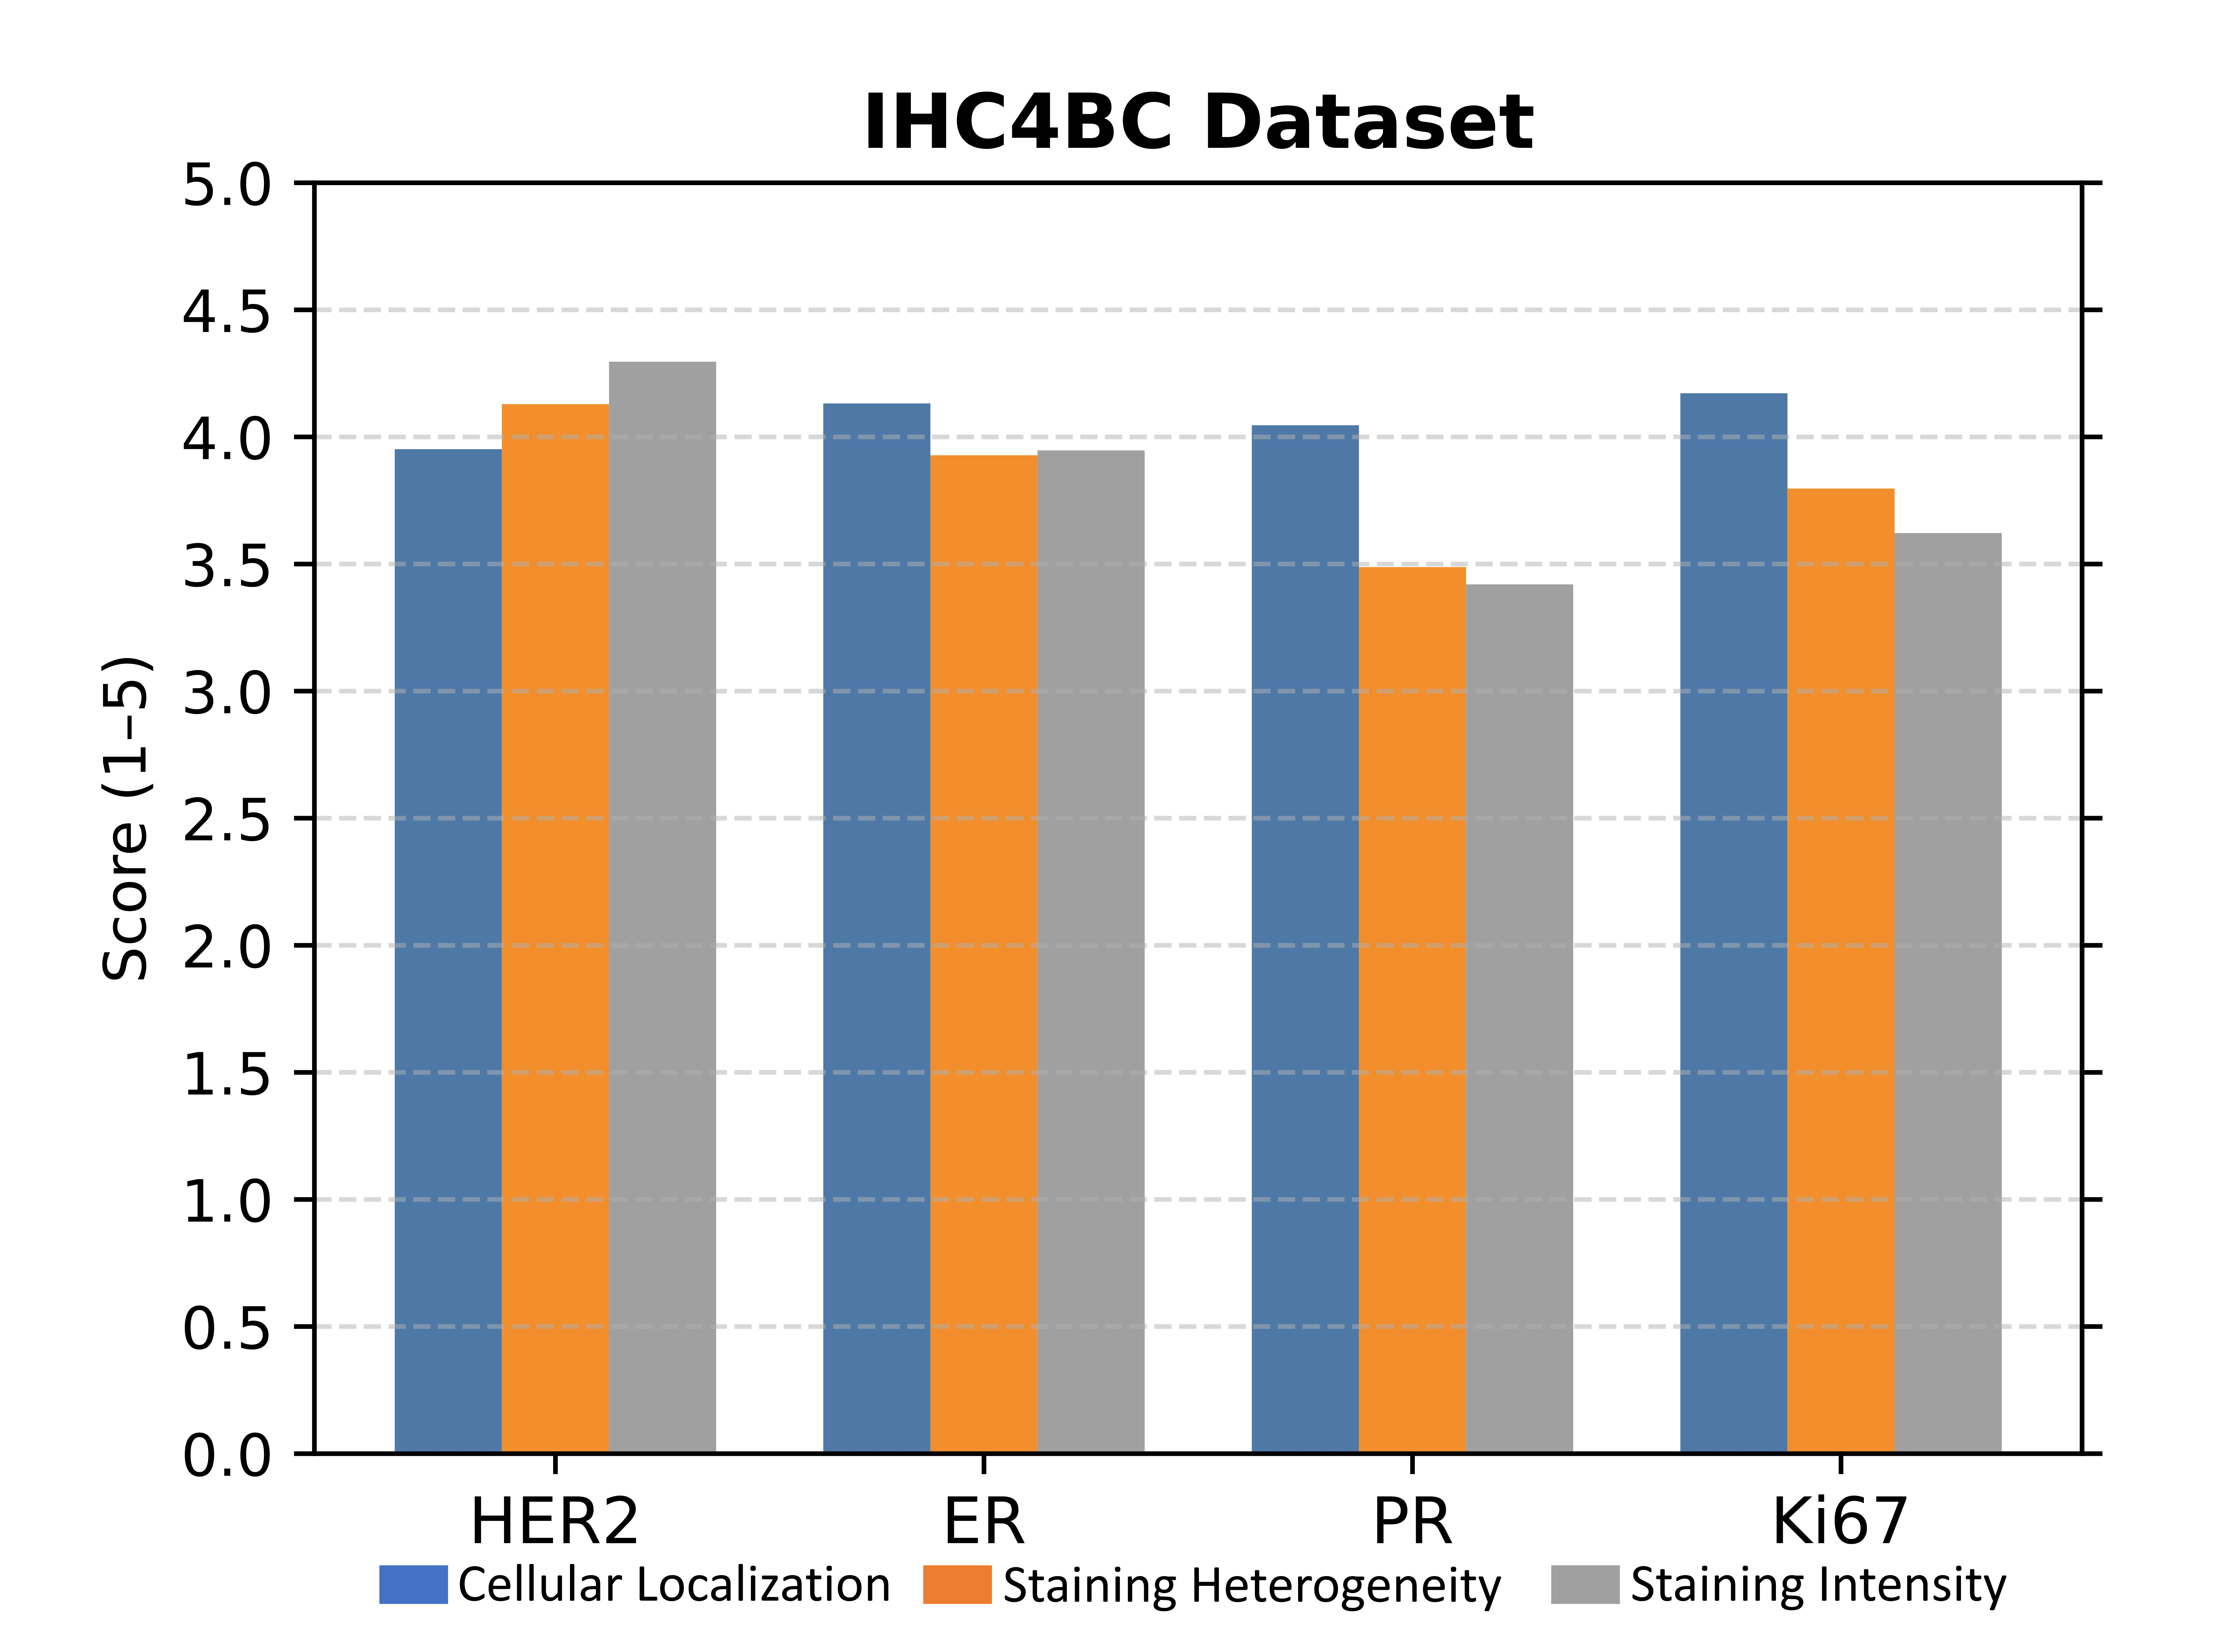
\includegraphics[width=\columnwidth]{image/qin9.png}}
\caption{{Pathologist evaluation of virtual IHC-stained images on the IHC4BC datasets across three criteria: cellular localization, staining heterogeneity, and staining intensity.}}
\label{qualitative_path_IHC4BC}
\end{figure}

\subsubsection{Unified Multiple IHC Virtual Staining Analysis}
% Fig. \ref{qualitative_3} demonstrates the virtual generation of HER2, ER, PR, and Ki67 stained images from H\&E stained images. It is evident that our network can achieve multi-stain transfer guided by different prompts. Notably, each stain exhibits its own distinct characteristics. For instance, the first image shows strong ER, PR and Ki67 expression but almost HER2 expression. The second image display strong ER and PR expression but minimal HER2 and Ki67 expression. 
% % The fourth image accurately capture the Ki67 expression.
% These results indicate that our method can precisely generate multiple IHC stains simultaneously, which is highly beneficial for the identification of breast cancer subtypes.
{Fig.~\ref{qualitative_3} shows the virtual generation of HER2, ER, PR, and Ki67 stained images from H\&E images, with each stain exhibiting distinct characteristics—for example, the first image shows strong ER, PR, and Ki67 but minimal HER2 expression, while the second shows strong ER and PR with low HER2 and Ki67. These results demonstrate that our method can generate multiple IHC stains simultaneously, aiding breast cancer subtype identification. The multiplex IHC images used for visualization are from the MIST dataset, which is mostly uniplex (\(\sim 77.8\%\)), with only a small fraction containing 2–4 stains.
}

\begin{figure}[t]
\centerline{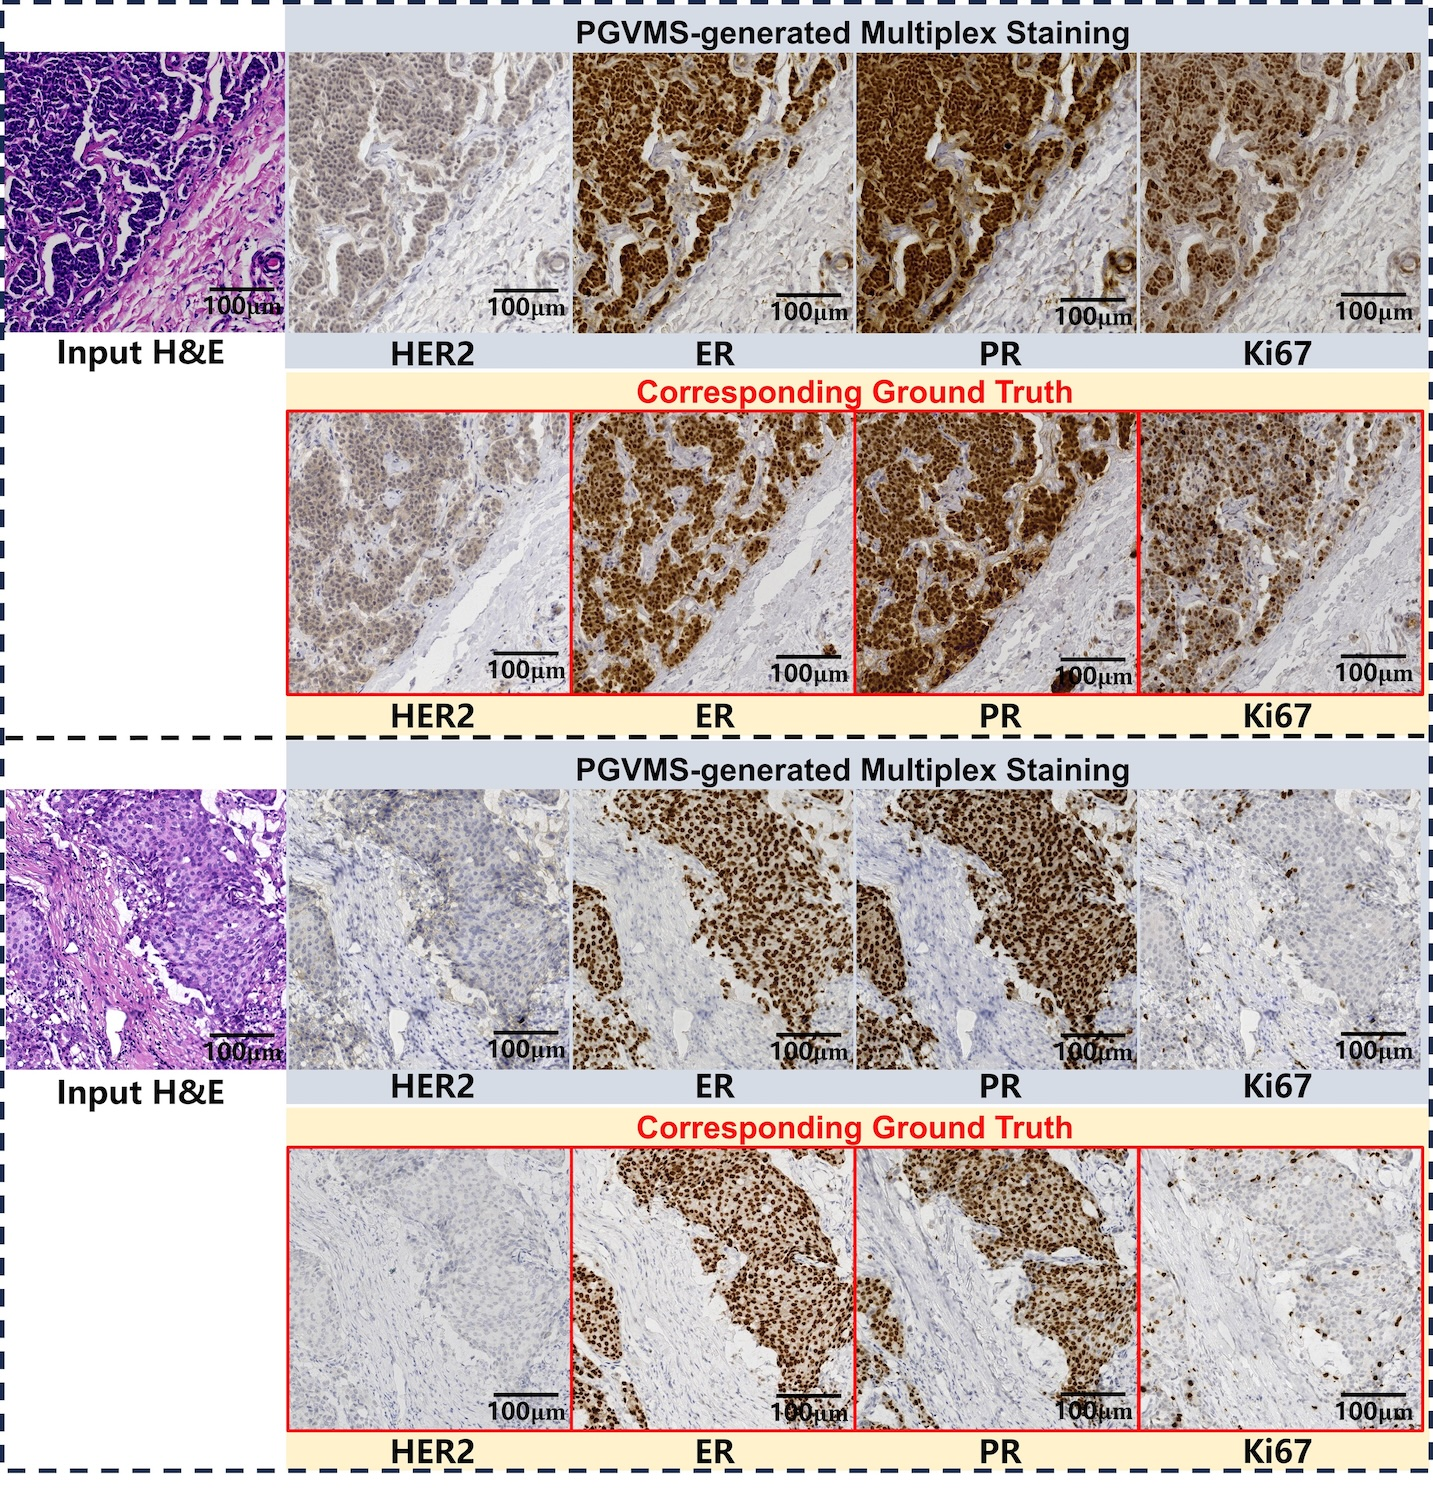
\includegraphics[width=\columnwidth]{image/qin10.jpg}}
\caption{\revision{Virtual multiplex IHC generation from H\&E-stained input images. For each H\&E input, the first row (gray background) displays PGVMS-generated staining for HER2, ER, PR, and Ki-67, and the second row (yellow background) shows the corresponding ground-truth IHC images.}}

\label{qualitative_3}
\end{figure}


\subsection{Ablation Study and Analysis}

\subsubsection{Module Ablation}
The proposed PGVMS accurately transforms H\&E-stained images into IHC-stained images through three core mechanisms: PALS, PCLS, and the PSSG generator. \revision{The baseline, built on the CUT framework, serves as an initial model for stain translation.} PALS ensures pathological consistency by preserving protein activation patterns, while PCLS enhances protein realism by enforcing semantic coherence across images. The PSSG generator enables prompt-driven adaptation for multi-stain tasks. Ablation experiments on the MIST dataset (Table \ref{tab:ablation_2}, pathology columns) reveal that PALS exerts a greater impact on pathological consistency. However, with PALS alone, protein characterization remains suboptimal. Consequently, PCLS improves perception metrics and enhances protein realism (Table \ref{tab:ablation_2}, perception columns) . When combined with PSSG’s semantic-embedded prompts, these components collectively achieve optimal stain transfer results, demonstrating PGVMS’s state-of-the-art virtual staining capability.


\begin{figure}[t]
\centerline{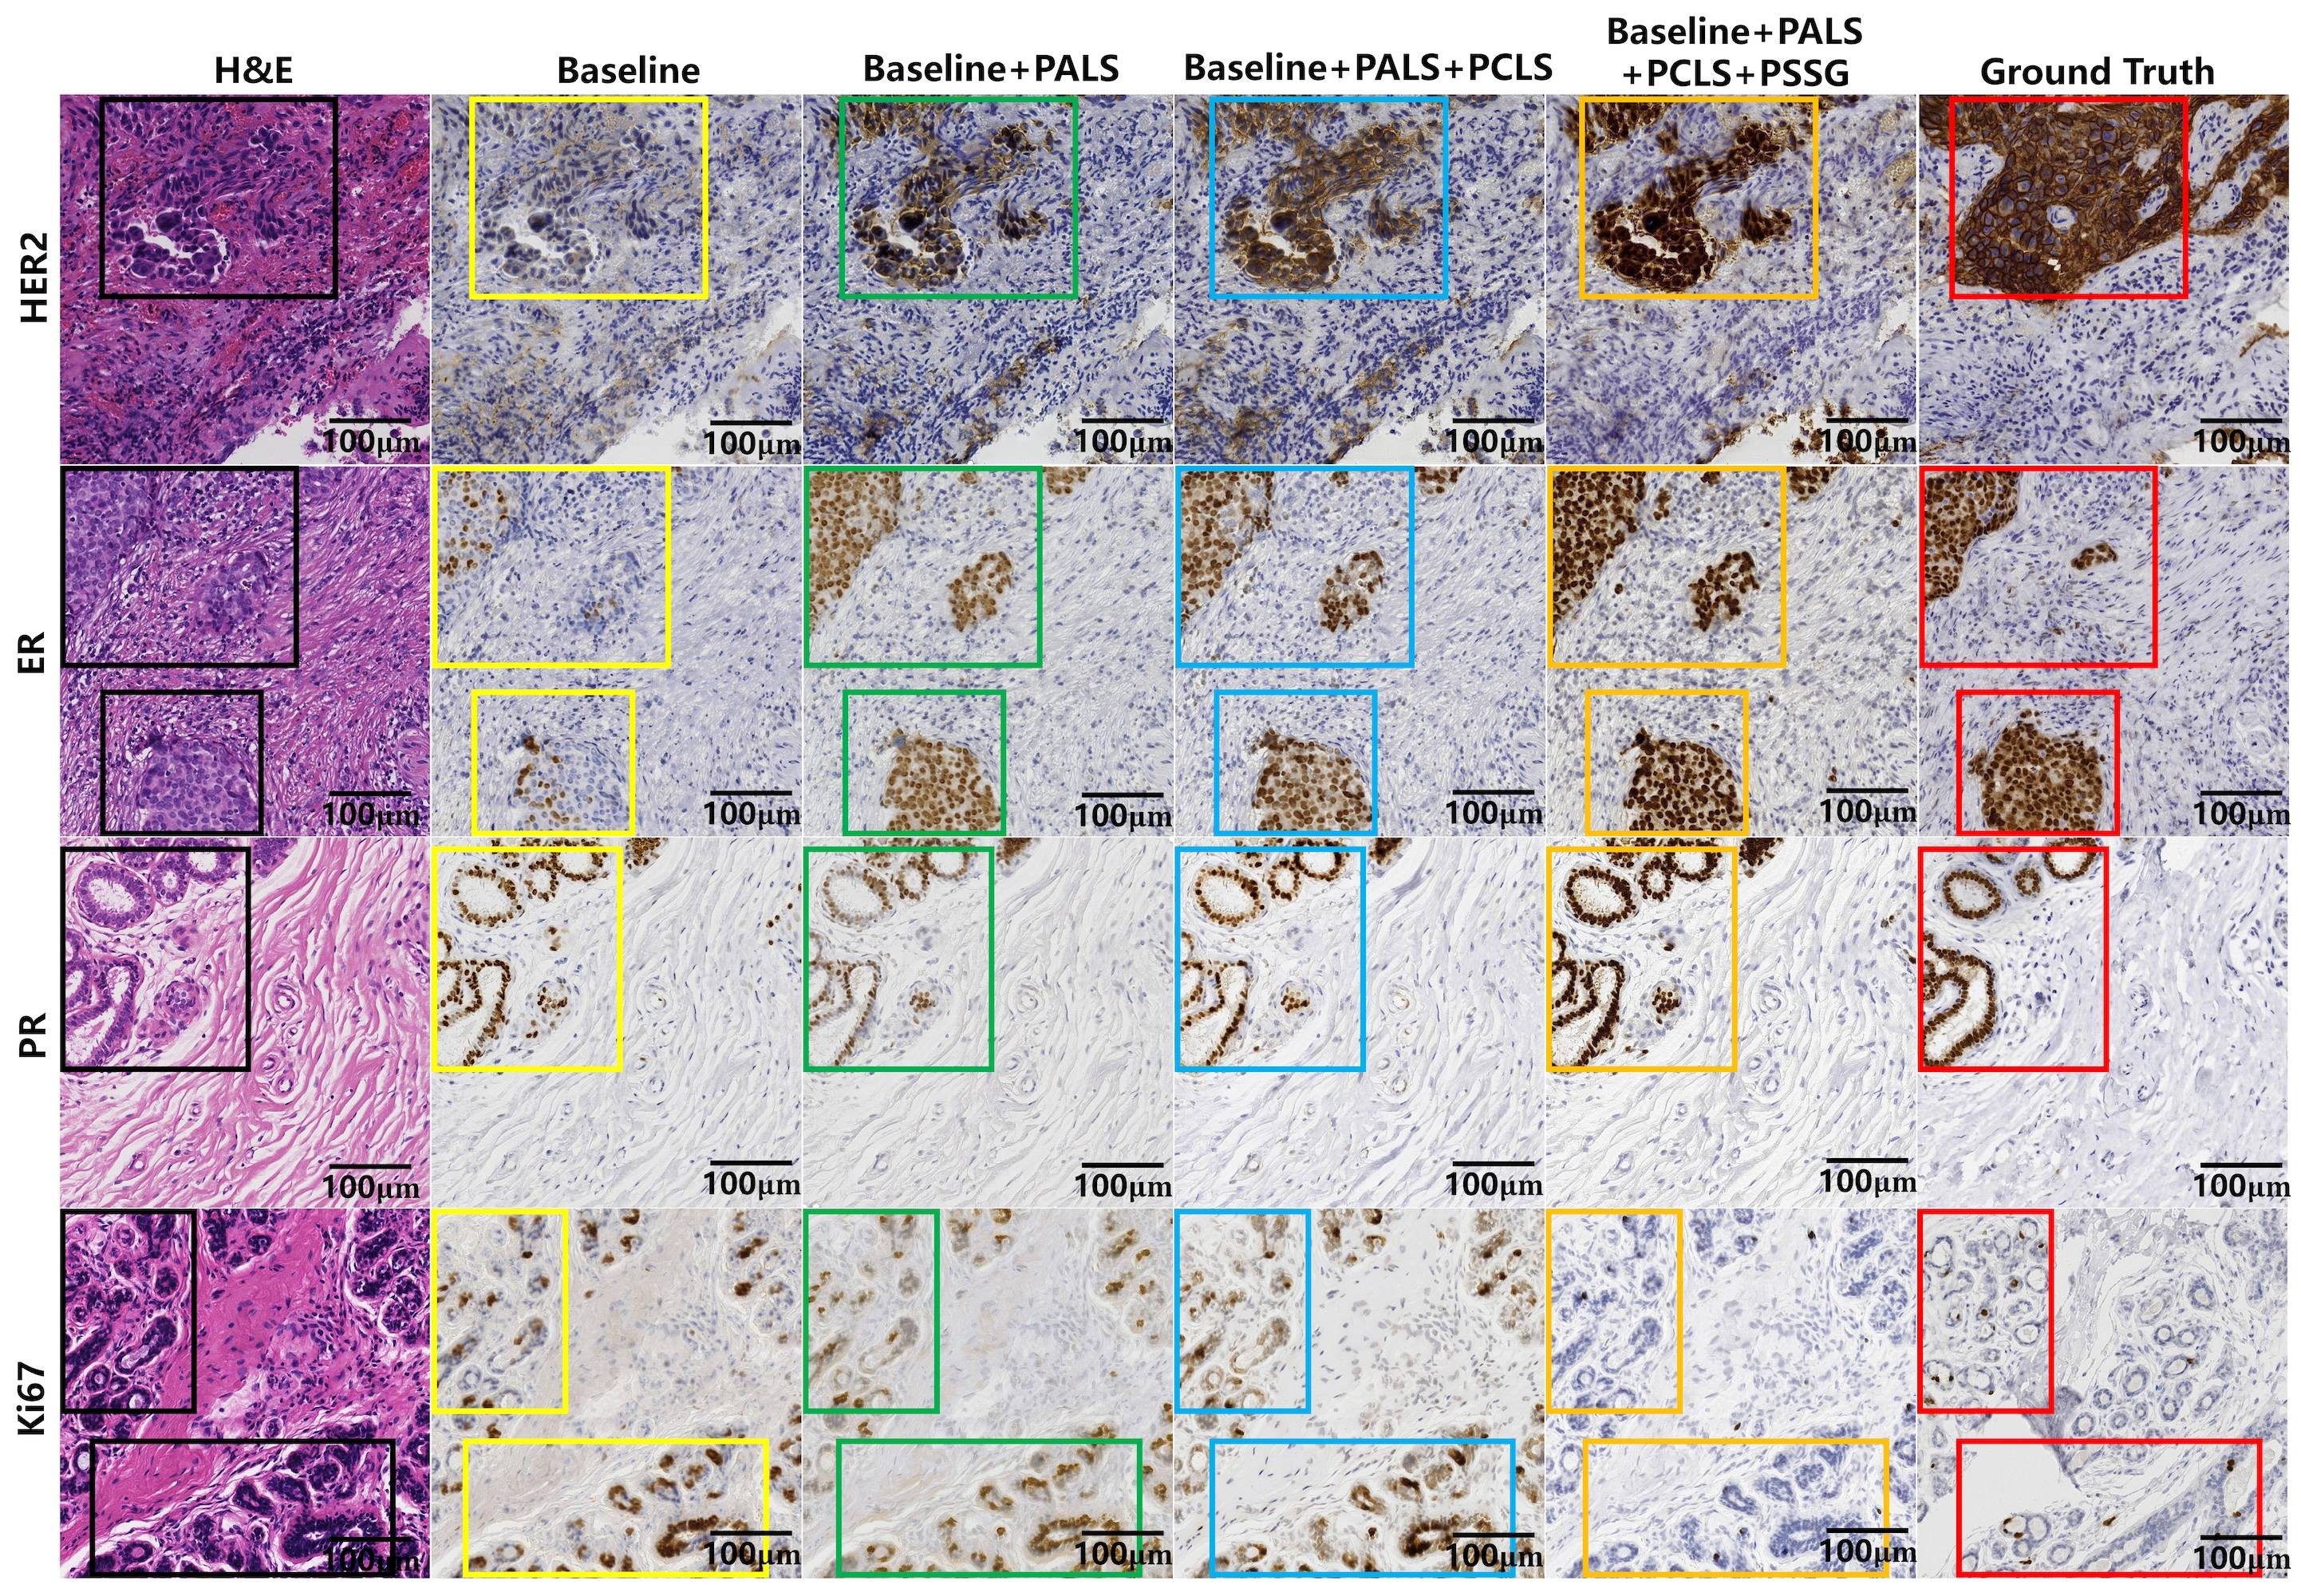
\includegraphics[width=\columnwidth]{image/qin11.jpg}}
\caption{\revision{Visualization of the effects of PALS, PCLS, and PSSG on our PGVMS. 
The color-coded rectangles indicate regions corresponding to different experimental configurations: black for the input H\&E image, yellow for the baseline output, green for baseline + PALS, blue for baseline + PALS + PCLS, orange for baseline + PALS + PCLS + PSSG, and red for the ground truth.}}
\label{ablation_1}
\end{figure}


% \begin{table}[hb]
%   \centering
%   \setlength\tabcolsep{2pt}
%   \renewcommand{\arraystretch}{1.0}
%   \caption{ABLATION STUDY OF STAIN TRANSFER PERFORMANCE ON MIST DATASET. THE BEST SCORES ARE HIGHLIGHTED IN BOLD.}
%   \label{tab:ablation_2}

%   \resizebox{\columnwidth}{!}{
%     \begin{tabular}{cccc|cc|cc|cc}
%       \Xhline{1.5pt} 
%       \multirow{2}{*}{Baseline} & \multirow{2}{*}{PSSG} & \multirow{2}{*}{PALS} & \multirow{2}{*}{PCLS} 
%       & \multicolumn{2}{c|}{Quality} & \multicolumn{2}{c|}{Pathology} & \multicolumn{2}{c}{Perception} \\
%       \cline{5-10}
%       & & & & PSNR$\uparrow$ & SSIM$\uparrow$ & IOD$_{\times10^7}$ & Pearson-R$\uparrow$ & FID$\downarrow$ & DISTS$\downarrow$ \\
%       \hline
%        $\checkmark$  &  &  & &
%       14.2183 & 0.2046 & -3.1237 & 0.6229 & 45.6044 & 0.2598 \\
%       $\checkmark$  &  & $\checkmark$ & &
%       \textbf{14.6252} & \textbf{0.2205} & -2.3128 & 0.8436 & 49.7711 & 0.2577 \\
      
%      $\checkmark$  &  & $\checkmark$ & $\checkmark$&
%       14.4773 & 0.2195 & -2.0626 & 0.8361 & 39.2908 & 0.2508 \\
      
%       $\checkmark$  & $\checkmark$ &  & &
%          13.7738  &0.1905   &-5.0098   & 0.3756 & 62.5494&0.2709 \\
%        $\checkmark$  & $\checkmark$ & $\checkmark$ & &
%       13.0808 & 0.1887  & -2.9507 &0.3998  &67.4985  &0.2813  \\
      
      
%       $\checkmark$  & $\checkmark$ & $\checkmark$ & $\checkmark$&
%       14.3421 & 0.2032 & \textbf{-0.3223} & \textbf{0.8649} & \textbf{38.0716} & \textbf{0.2343} \\
%       \Xhline{1.5pt} 
%     \end{tabular}
%   }
% \end{table}

% % % % % % % % % % % % % % % % % % % % % % % % % % 
\begin{table}[!htbp]
  \centering
  \setlength\tabcolsep{2pt}
  \renewcommand{\arraystretch}{1.0}
  \caption{{ABLATION STUDY OF STAIN TRANSFER PERFORMANCE ON MIST DATASET. THE BEST SCORES ARE HIGHLIGHTED IN BOLD.}}
  \label{tab:ablation_2}

  \resizebox{\columnwidth}{!}{
    \begin{tabular}{cccc|cc|cc|cc}
      \Xhline{1.5pt} 
      \multirow{2}{*}{Baseline} & \multirow{2}{*}{PALS} & \multirow{2}{*}{PCLS} & \multirow{2}{*}{PSSG} 
      & \multicolumn{2}{c|}{Quality} & \multicolumn{2}{c|}{Pathology} & \multicolumn{2}{c}{Perception} \\
      \cline{5-10}
      & & & & PSNR$\uparrow$ & SSIM$\uparrow$ & IOD$_{\times10^7}$ & Pearson-R$\uparrow$ & FID$\downarrow$ & DISTS$\downarrow$ \\
      \hline
       $\checkmark$  &  &  & &
      14.2183 & 0.2046 & -3.1237 & 0.6229 & 45.6044 & 0.2598 \\
      $\checkmark$  & $\checkmark$ &  & &
      \textbf{14.6252} & \textbf{0.2205} & -2.3128 & 0.8436 & 49.7711 & 0.2577 \\
      
     $\checkmark$  & $\checkmark$ & $\checkmark$ & &
      14.4773 & 0.2195 & -2.0626 & 0.8361 & 39.2908 & 0.2508 \\
      
      $\checkmark$  &  &  & $\checkmark$&
         13.7738  &0.1905   &-5.0098   & 0.3756 & 62.5494&0.2709 \\
       $\checkmark$  & $\checkmark$ &  & $\checkmark$&
      13.0808 & 0.1887  & -2.9507 &0.3998  &67.4985  &0.2813  \\
      
      
      $\checkmark$  & $\checkmark$ & $\checkmark$ & $\checkmark$&
      14.3421 & 0.2032 & \textbf{-0.3223} & \textbf{0.8649} & \textbf{38.0654} & \textbf{0.2343} \\
      \Xhline{1.5pt} 
    \end{tabular}
  }
\end{table}
% % % % % % % % % % % % % % % % % % % % % % % % % % 
% \begin{table}[hb]
%   \centering
%   \setlength\tabcolsep{2pt}
%   \renewcommand{\arraystretch}{1.0}
%   \caption{ABLATION STUDY OF STAIN TRANSFER PERFORMANCE ON MIST DATASET. THE BEST SCORES ARE HIGHLIGHTED IN BOLD.}
%   \label{tab:ablation_2}

%   \resizebox{\columnwidth}{!}{
%     \begin{tabular}{c|cc|cc|cc}
%       \Xhline{1.5pt} 
%       \multirow{2}{*}{Method} 
%       & \multicolumn{2}{c|}{Quality} & \multicolumn{2}{c|}{Pathology} & \multicolumn{2}{c}{Perception} \\
%       \cline{2-7}
%       & PSNR$\uparrow$ & SSIM$\uparrow$ & IOD$_{\times10^7}$ & Pearson-R$\uparrow$ & FID$\downarrow$ & DISTS$\downarrow$ \\
%       \hline
%       Baseline  & 
%       14.2183 & 0.2046 & -3.1237 & 0.6229 & 45.6044 & 0.2598 \\
      
%       Baseline+PALS & 
%       \textbf{14.6252} & \textbf{0.2205} & -2.3128 & 0.8436 & 49.7711 & 0.2577 \\
      
%       Baseline+PALS+PCLS & 
%       14.4773 & 0.2195 & -2.0626 & 0.8361 & 39.2908 & 0.2508 \\
      
%        Baseline+PALS+PCLS+PSSG  & 
%       14.3421 & 0.2032 & \textbf{-0.3223} & \textbf{0.8649} & \textbf{38.0716} & \textbf{0.2343} \\
%       \Xhline{1.5pt} 
%     \end{tabular}
%   }
% \end{table}


%  \begin{table}[hb]
%   \centering
%   \setlength\tabcolsep{2pt}
%   \renewcommand{\arraystretch}{1.0}
%   \caption{ABLATION OF STAIN TRANSFER PERFORMANCE ON MIST DATASETS. THE BEST SCORES ARE IN BOLD, RESPECTIVELY}
%   \label{tab:ablation_2}

%   \resizebox{\columnwidth}{!}{
%     \begin{tabular}{c|cc|cc|cc}
%       \Xhline{1.5pt} 
%       \multirow{2}{*}{Method} 
%       & \multicolumn{2}{c|}{Pathology} & \multicolumn{2}{c|}{Quality} & \multicolumn{2}{c}{Perception} \\
%       \cline{2-7}
%       & IOD$_{\times10^7}$ & Pearson-R$\uparrow$ & PSNR$\uparrow$  & SSIM$\uparrow$  & FID$\downarrow$ &  DISTS$\downarrow$ \\
%       \hline
%       Baseline  & 
%        -3.1237 & 0.6229 & 14.2183 & 0.2046 & 45.6044  & 0.2598 \\
      
%       Baseline+PALS & 
%        -2.3128 & 0.8436 & \textbf{14.6252} & \textbf{0.2205} & 49.7711  & 0.2577 \\
      
%       Baseline+PALS+PCLS & 
%        -2.0626 & 0.8361 & 14.4773 & 0.2195 & 39.2908  & 0.2508 \\
      
%       PGVMS & 
%       \textbf{-0.3223} & \textbf{0.8649} & 14.3421 & 0.2032 & \textbf{38.0716} & \textbf{0.2343} \\
%       \Xhline{1.5pt} 
%     \end{tabular}
%   }
% \end{table}








% \begin{table}[h!]
% \centering
% \caption{Average Performance Across All Stain Types}
% \label{tab:mean_results}
% \begin{tabular}{c|ccccc}
% \Xhline{1.5pt} 
% \{Parameter} & \textbf{IOD} & \textbf{Pearson-R} & \textbf{PSNR} & \textbf{SSIM} & \textbf{FID} & \textbf{DISTS} \\
% \hline
% 1.0 & -1.9404 & 0.8284 & 14.4570 & 0.2089 & 39.7054 & 0.2427 \\
% 1.4 & -3.8249 & 0.7575 & 14.6659 & 0.2207 & 44.4903 & 0.2371 \\
% 1.8 & -0.3223 & 0.8649 & 14.3421 & 0.2032 & 38.0654 & 0.2344 \\
% 2.2 & -1.8733 & 0.8507 & 14.2708 & 0.2197 & 43.6559 & 0.2449 \\
% \Xhline{1.5pt} 
% \end{tabular}
% \end{table}








% \begin{table*}[ht]
% \centering
% \caption{Feature-level FID between virtual IHC and ground-truth IHC computed using the pathology foundation model CONCH. Lower values indicate better alignment. \textbf{The best and second-best results are highlighted in bold and underlined, respectively.}}
% \label{tab:combined_fid_conch_5}
% \setlength\tabcolsep{4pt}
% \renewcommand{\arraystretch}{1.15}
% \resizebox{\textwidth}{!}{
% \begin{tabular}{l|cccc|c||cccc|c}
% \Xhline{1.3pt}
% \multirow{2}{*}{Method} 
% & \multicolumn{5}{c||}{\textbf{MIST}} 
% & \multicolumn{5}{c}{\textbf{IHC4BC}} \\
% \cline{2-11}
% & HER2 & ER & PR & Ki67 & Mean 
% & HER2 & ER & PR & Ki67 & Mean \\
% \hline
% CycleGAN   & 102.1581 & 52.9350 & 125.7399 & 48.0381 & 82.2178 & 218.4938 & 44.1311 & 81.4923 & 49.0361 & 98.2884 \\
% Pix2Pix    & 95.9983 & 189.5522 & 182.9658 & 216.5276 & 171.2610 & 153.2364 & 105.1925 & 95.7887 & 128.3961 & 120.6534 \\
% CUT        & 62.6960 & 39.4071 & \underline{32.4882} & 35.4223 & 42.5034 & 80.8654 & 32.3410 & 39.4285 & 247.6296 & 100.0661 \\
% ASP        & \underline{39.9833} & 52.4421 & 38.3425 & 43.7905 & 43.6396 & 76.8791 & \underline{25.4769} & \underline{31.9873} & \textbf{20.9709} & \underline{38.8285} \\
% Pyramid    & 151.2503 & 153.7980 & 145.9719 & 172.3845 & 155.8512 & 237.9637 & 172.1971 & 162.0819 & 106.7118 & 169.7386 \\
% TDKStain   & 85.3784 & 73.2279 & 98.2533 & 143.9924 & 100.2130 & \underline{49.5412} & 61.5834 & 75.3190 & 52.3977 & 59.7103 \\
% PSPStain   & \textbf{34.7499} & \textbf{30.8958} & 32.7645 & \textbf{26.2759} & \textbf{31.1715} & \textbf{47.1362} & 35.2759 & 48.1594 & 36.9802 & 41.8879 \\
% DDBM       & 291.1494 & 281.9772 & 244.6667 & 215.1843 & 258.2444 & 326.7613 & 256.5512 & 258.2804 & 182.5962 & 256.0473 \\
% UNSB       & 61.9792 & 38.1701 & 49.4495 & 36.9417 & 46.6351 & 64.6003 & 69.6588 & 37.2139 & 48.7528 & 55.0565 \\
% ControlNet & 283.2979 & 253.5201 & 317.4814 & 490.4310 & 336.1826 & 322.7134 & 432.5187 & 455.0586 & 434.0198 & 411.0776 \\
% VIMs       & 353.5241 & 240.2728 & 234.2091 & 233.9704 & 265.4941 & 192.7621 & 140.0983 & 177.3091 & 166.0101 & 169.0449 \\
% UMDST      & 154.3398 & 168.4891 & 147.7141 & 254.2693 & 181.2031 & 98.5943 & 116.0732 & 100.4608 & 184.7146 & 124.9607 \\
% \textbf{PGVMS} 
% & 55.1115 & \underline{31.0460} & \textbf{23.5529} & \underline{29.5545} & \underline{34.8162} 
% & 61.7747 & \textbf{24.5485} & \textbf{30.8413} & \underline{21.8956} & \textbf{34.7650} \\
% \Xhline{1.3pt}
% \end{tabular}
% }
% \end{table*}



% \subsection{Ablation Study and Analysis}
To further explore the visual effects of the PCLS, PALS, and PSSG generator  on virtual IHC image generation, we present qualitative ablation results in Fig. \ref{ablation_1}. As shown in Fig. \ref{ablation_1}, without the constraints of PALS and PCLS, the model fails to fully utilize the supervisory information provided by adjacent layer IHC images (yellow), resulting in inaccurate pathological characteristics, such as misstained nuclei or cell membranes. PALS effectively maintains the pathological consistency of the generated images by preserving molecular-level protein activation patterns (green), ensuring that the virtual staining aligns with biological reality. PCLS enhances the realism of the generated tumor regions by enforcing cross-image semantic topology consistency (blue), mitigating spatial misalignment and improving inter-image coherence. PSSG generator enables prompt-driven semantic embedding adaptation across multiple staining tasks (orange), enhancing pathological semantic embedding. When PALS and PCLS are added, the performance improves, but some staining inaccuracies remain, and certain nuclei are still incorrectly stained. When the PSSG generator, PALS, and PCLS are applied simultaneously, the virtual IHC images closely resemble the referenced adjacent layer IHC images (red), achieving the best staining transfer performance.
% This synergistic integration of the PSSG generator, PALS, and PCLS establishes PGVMS as a state-of-the-art solution for virtual staining in computational pathology.




%  \begin{table}[ht]
%   \centering
%   \setlength\tabcolsep{2pt}
%   \renewcommand{\arraystretch}{1.0}
%   \caption{ABLATION OF FOD $\alpha$ ON MIST DATASETS. THE BEST AND SECOND BEST SCORES ARE IN BOLD, RESPECTIVELY}
%   \label{tab:ablation_OD}

%   \resizebox{\columnwidth}{!}{
%     \begin{tabular}{c|cc|cc|cc}
%       \Xhline{1.5pt} 
%       \multirow{2}{*}{FOD $\alpha$} 
%       & \multicolumn{2}{c|}{Pathology} & \multicolumn{2}{c|}{Quality} & \multicolumn{2}{c}{Perception} \\
%       \cline{2-7}
%       & IOD$_{\times10^7}$ & Pearson-R$\uparrow$ & PSNR$\uparrow$ & SSIM$\uparrow$ & FID$\downarrow$  & DISTS$\downarrow$ \\
%       \hline
%      1.0 & -2.2031 & 0.8331 & 14.6189 & 0.2115 & 43.8208 & 0.2395 \\
% 1.4 &-1.7750 & 0.8598 & \textbf{14.6242} & 0.2078 & 38.3692 & 0.2372 \\
% 1.8 & \textbf{-0.3223} & \textbf{0.8649} & 14.3421 & 0.2032 & \textbf{38.0654} & \textbf{0.2344} \\
% 2.2 & -1.8733 & 0.8507 & 14.2708 & \textbf{0.2197} & 43.6559 & 0.2449 \\
%       \Xhline{1.5pt} 
%     \end{tabular}
%   }
% \end{table}







\subsubsection{Guidance Mechanism}
To evaluate how pathological semantic prompts operate within the PSSG generator, we replaced the CONCH model with one-hot encoding guidance and CLIP model guidance. As shown in the Table \ref{tab:ablation_CONCH_}, the minimal IOD indicates superior protein expression consistency, while the relatively low yet high absolute Pearson-R score reflects consistent tumor expression patterns. The outstanding perception metrics demonstrate optimal visual diagnostic fidelity, highlighting CONCH's capability to deliver robust pathological semantic embeddings for virtual multiplex IHC staining within a unified model.

\begin{table}[!htbp]
  \centering
  \setlength\tabcolsep{2pt}
  \renewcommand{\arraystretch}{1.0}
  \caption{\revision{ABLATION STUDY OF GUIDANCE MECHANISM ON MIST DATASET. THE BEST SCORES ARE HIGHLIGHTED IN BOLD.}}
  \label{tab:ablation_CONCH_}

  \resizebox{\columnwidth}{!}{
    \begin{tabular}{c|cc|cc|cc}
      \Xhline{1.5pt} 
      \multirow{2}{*}{ Guidance} 
      & \multicolumn{2}{c|}{Quality} & \multicolumn{2}{c|}{Pathology} & \multicolumn{2}{c}{Perception} \\
      \cline{2-7}
      & PSNR$\uparrow$ & SSIM$\uparrow$ & IOD$_{\times10^7}$ & Pearson-R$\uparrow$ & FID$\downarrow$ & DISTS$\downarrow$ \\
      \hline
     One Hot & \textbf{14.9029} & \textbf{0.2310} & -2.1429 & \textbf{0.8729} & 38.5514 & 0.2379 \\
     CLIP & 14.2745 & 0.1895 & -1.4198 & 0.8678 & 39.2263 & 0.2454 \\
     % PLIP & 14.5181 & 0.2100 & -1.9039 & 0.8357 & 40.9981 & 0.2398 \\
     % MUSK & 14.7346 & 0.2089 & -2.5387 & 0.8409 & 40.6993 & 0.2499 \\
     CONCH & 14.3421 & 0.2032 & \textbf{-0.3223} & 0.8649 & \textbf{38.0654} & \textbf{0.2344} \\
      \Xhline{1.5pt} 
    \end{tabular}
  }
\end{table}

\subsubsection{Image-Guided Bias Effectiveness} {We evaluated the effect of incorporating instance-specific image-derived bias into the text prompt. As shown in Table~\ref{tab:ablation_bias_mechanism}, adding the bias consistently improves pathology, quality, and perception metrics across all biomarkers, indicating that it enhances semantic alignment and preserves domain-specific features in the virtual stains.}

\begin{table}[!htbp]
  \centering
  \setlength\tabcolsep{2pt}
  \renewcommand{\arraystretch}{1.0}
  \caption{{ABLATION STUDY OF IMAGE-GUIDED BIAS MECHANISM ON MIST DATASET. THE BEST SCORES ARE HIGHLIGHTED IN BOLD.}}
  \label{tab:ablation_bias_mechanism}

  \resizebox{\columnwidth}{!}{
    \begin{tabular}{c|cc|cc|cc}
      \Xhline{1.5pt} 
      \multirow{2}{*}{Method} 
      & \multicolumn{2}{c|}{Quality} & \multicolumn{2}{c|}{Pathology} & \multicolumn{2}{c}{Perception} \\
      \cline{2-7}
      & PSNR$\uparrow$ & SSIM$\uparrow$ & IOD$_{\times10^7}$ & Pearson-R$\uparrow$ & FID$\downarrow$ & DISTS$\downarrow$ \\
      \hline
      w/o bias & 14.0289 & \textbf{0.2099} & -2.2577 & 0.7400 & 58.2488 & 0.2482 \\
      w/ bias & \textbf{14.3421} & 0.2062 & \textbf{-0.3223} & \textbf{0.8648} & \textbf{38.0654} & \textbf{0.2344} \\
      \Xhline{1.5pt} 
    \end{tabular}
  }
\end{table}

\subsubsection{Pooling Strategy in Bias Computation}
 {We compared max pooling, average pooling, and a combination of both for extracting the image-guided bias. Table~\ref{tab:ablation_pooling_avg} shows that combining max and average pooling outperforms either operation alone, suggesting that fusing localized discriminative cues with global contextual information provides a more informative and balanced bias for guiding the virtual staining.}


\begin{table}[ht]
  \centering
  \setlength\tabcolsep{2pt}
  \renewcommand{\arraystretch}{1.0}
  \caption{{ABLATION STUDY OF POOLING STRATEGY ON MIST DATASET. THE BEST SCORES ARE HIGHLIGHTED IN BOLD.}}
  \label{tab:ablation_pooling_avg}

  \resizebox{\columnwidth}{!}{
    \begin{tabular}{c|cc|cc|cc}
      \Xhline{1.5pt} 
      \multirow{2}{*}{Pooling Strategy} 
      & \multicolumn{2}{c|}{Quality} & \multicolumn{2}{c|}{Pathology} & \multicolumn{2}{c}{Perception} \\
      \cline{2-7}
      & PSNR$\uparrow$ & SSIM$\uparrow$ & IOD$_{\times10^7}$ & Pearson-R$\uparrow$ & FID$\downarrow$ & DISTS$\downarrow$ \\
      \hline
      Only Maxpooling & 14.5682 & \textbf{0.2184} & -1.7611 & 0.7890 & 53.5903 & 0.2522 \\
      Only Avgpooling & \textbf{14.6032} & 0.2086 & -2.4378 & 0.7607 & 83.3022 & 0.2646 \\
      Max \& Avg Pooling & 14.3421 & 0.2032 & \textbf{-0.3223} & \textbf{0.8648} & \textbf{38.0654} & \textbf{0.2344} \\
      \Xhline{1.5pt} 
    \end{tabular}
  }
\end{table}
\subsubsection{Fusion Strategy in PGSN}
{We ablated the prompt guidance style normalization (PGSN) against simple addition and cross-attention between the prompt and image feature. Table~\ref{tab:ablation_fusion_1} demonstrates that PGSN substantially outperforms these alternatives by adaptively modulating text embeddings with image-derived statistics, leading to stronger semantic alignment and better preservation of pathology-specific features.}







\begin{table}[!htbp]
  \centering
  \setlength\tabcolsep{2pt}
  \renewcommand{\arraystretch}{1.0}
  \caption{\revision{ABLATION STUDY OF FUSION MECHANISM ON MIST DATASET. THE BEST SCORES ARE HIGHLIGHTED IN BOLD.}}
  \label{tab:ablation_fusion_1}

  \resizebox{\columnwidth}{!}{
    \begin{tabular}{c|cc|cc|cc}
      \Xhline{1.5pt} 
      \multirow{2}{*}{ Guidance} 
      & \multicolumn{2}{c|}{Quality} & \multicolumn{2}{c|}{Pathology} & \multicolumn{2}{c}{Perception} \\
      \cline{2-7}
      & PSNR$\uparrow$ & SSIM$\uparrow$ & IOD$_{\times10^7}$ & Pearson-R$\uparrow$ & FID$\downarrow$ & DISTS$\downarrow$ \\
      \hline
     Addition & 13.8117 & 0.1904 & -1.5385 & 0.7942 & 53.1891 & 0.2451 \\
     Cross Attention & 13.8461 & 0.2028 & -2.4021 & 0.8041 & 55.5236 & 0.2438 \\
     PGSN & \textbf{14.3421} & \textbf{0.2032} & \textbf{-0.3223} & \textbf{0.8649} & \textbf{38.0654} & \textbf{0.2344} \\
      \Xhline{1.5pt} 
    \end{tabular}
  }
\end{table}


% \begin{table}[ht]
%   \centering
%   \setlength\tabcolsep{2pt}
%   \renewcommand{\arraystretch}{1.0}
%   \caption{ABLATION STUDY OF FUSION STRATEGY ON MIST DATASET. THE BEST SCORES ARE HIGHLIGHTED IN BOLD.}
%   \label{tab:ablation_fusion_avg}

%   \resizebox{\columnwidth}{!}{
%     \begin{tabular}{c|cc|cc|cc}
%       \Xhline{1.5pt} 
%       \multirow{2}{*}{Fusion Strategy} 
%       & \multicolumn{2}{c|}{Quality} & \multicolumn{2}{c|}{Pathology} & \multicolumn{2}{c}{Perception} \\
%       \cline{2-7}
%       & PSNR$\uparrow$ & SSIM$\uparrow$ & IOD$_{\times10^7}$ & Pearson-R$\uparrow$ & FID$\downarrow$ & DISTS$\downarrow$ \\
%       \hline
%       Addition & 13.8117 & 0.1904 & -1.5375 & 0.7942 & 53.1891 & 0.2451 \\
%       Cross Attention & 13.8461 & 0.2028 & -2.4021 & 0.8041 & 55.5236 & 0.2483 \\
%       PGSN & \textbf{14.3421} & \textbf{0.2032} & \textbf{-0.3223} & \textbf{0.8649} & \textbf{38.0654} & \textbf{0.2344} \\
%       \Xhline{1.5pt} 
%     \end{tabular}
%   }
% \end{table}

\subsubsection{Normalization Strategy}
 {We assessed the role of instance normalization (IN) and layer normalization (LN) within PGSN. Table~\ref{tab:ablation_normalization_avg} shows that using both IN and LN achieves the best overall performance, as IN suppresses irrelevant style variations while LN stabilizes global feature distributions, resulting in more accurate and consistent virtual staining.}


\begin{table}[!htbp]
  \centering
  \setlength\tabcolsep{2pt}
  \renewcommand{\arraystretch}{1.0}
  \caption{{ABLATION STUDY OF NORMALIZATION STRATEGY ON MIST DATASET. THE BEST SCORES ARE HIGHLIGHTED IN BOLD.}}
  \label{tab:ablation_normalization_avg}

  \resizebox{\columnwidth}{!}{
    \begin{tabular}{c|cc|cc|cc}
      \Xhline{1.5pt} 
      \multirow{2}{*}{Normalization Strategy} 
      & \multicolumn{2}{c|}{Quality} & \multicolumn{2}{c|}{Pathology} & \multicolumn{2}{c}{Perception} \\
      \cline{2-7}
      & PSNR$\uparrow$ & SSIM$\uparrow$ & IOD$_{\times10^7}$ & Pearson-R$\uparrow$ & FID$\downarrow$ & DISTS$\downarrow$ \\
      \hline
      Only IN & 14.4614 & 0.2184 & -3.2292 & 0.7939 & 69.9662 & 0.2600 \\
      Only LN & \textbf{15.6425} & \textbf{0.2887} & -3.9779 & 0.7672 & 153.7774 & 0.3414 \\
      Both IN\&LN & 14.3421 & 0.2032 & \textbf{-0.3223} & \textbf{0.8649} & \textbf{38.0654} & \textbf{0.2344} \\
      \Xhline{1.5pt} 
    \end{tabular}
  }
\end{table}

\subsubsection{Sensitivity Analysis of $\alpha$ in MLPA}
To investigate the influence of $\alpha$ in MLPA, we conducted an ablation study with different values ($\alpha$=1.0, 1.4, 1.8, 2.2) in Table \ref{tab:ablation_OD}. The results demonstrate a bell-shaped performance curve, where $\alpha$=1.8 achieves optimal balance between molecular expression accuracy and histological structure preservation.
%, outperforming other configurations across all metrics

\begin{table}[ht]
  \centering
  \setlength\tabcolsep{2pt}
  \renewcommand{\arraystretch}{1.0}
  \caption{\revision{ABLATION STUDY OF FOD $\alpha$ ON MIST DATASET. THE BEST SCORES ARE HIGHLIGHTED IN BOLD.}}
  \label{tab:ablation_OD}

  \resizebox{\columnwidth}{!}{
    \begin{tabular}{c|cc|cc|cc}
      \Xhline{1.5pt} 
      \multirow{2}{*}{FOD $\alpha$} 
      & \multicolumn{2}{c|}{Quality} & \multicolumn{2}{c|}{Pathology} & \multicolumn{2}{c}{Perception} \\
      \cline{2-7}
      & PSNR$\uparrow$ & SSIM$\uparrow$ & IOD$_{\times10^7}$ & Pearson-R$\uparrow$ & FID$\downarrow$ & DISTS$\downarrow$ \\
      \hline
     1.0 & 14.6189 & 0.2115 & -2.2031 & 0.8331 & 43.8208 & 0.2395 \\
     1.4 & \textbf{14.6242} & 0.2078 & -1.7750 & 0.8598 & 38.3692 & 0.2372 \\
     1.8 & 14.3421 & 0.2032 & \textbf{-0.3223} & \textbf{0.8649} & \textbf{38.0654} & \textbf{0.2344} \\
     2.2 & 14.2708 & \textbf{0.2197} & -1.8733 & 0.8507 & 43.6559 & 0.2449 \\
      \Xhline{1.5pt} 
    \end{tabular}
  }
\end{table}


% \begin{table*}[!htbp]
%   \centering
%   \setlength\tabcolsep{5pt}
%   \renewcommand{\arraystretch}{1}
%   \caption{Ablation on the pathology foundation model used in PGSN. Comparison between \textit{PLIP}, \textit{MUSK} and \textit{CONCH}. The best results are in bold.}
%   \label{tab:ablation_foundation_1}
%   \resizebox{\textwidth}{!}{
%     \begin{tabular}{c|cc|cc|cc|cc|cc|cc}
%       \Xhline{1.5pt}
%       \multirow{3}{*}{Model} &
%       \multicolumn{6}{c|}{HER2} & \multicolumn{6}{c}{ER} \\
%       \cline{2-13}
%       & \multicolumn{2}{c|}{Pathology} & \multicolumn{2}{c|}{Quality (reference)} & \multicolumn{2}{c|}{Perception} &
%       \multicolumn{2}{c|}{Pathology} & \multicolumn{2}{c|}{Quality (reference)} & \multicolumn{2}{c}{Perception} \\
%       \cline{2-13}
%       & IOD${\times10^7}$ & Pearson-R$\uparrow$ & PSNR$\uparrow$ & SSIM$\uparrow$ & FID$\downarrow$ & DISTS$\downarrow$
%       & IOD${\times10^7}$ & Pearson-R$\uparrow$ & PSNR$\uparrow$ & SSIM$\uparrow$ & FID$\downarrow$ & DISTS$\downarrow$ \\
%       \hline
%       PLIP &
%       \textbf{-0.3509} & 0.8151 & 14.2185 & 0.1872 & 49.0771 & 0.2504 &
%       +1.7450 & \textbf{0.9022} & 14.0899 & \textbf{0.2103} & 46.8715 & 0.2528 \\
%       MUSK &
%       -4.1039 & 0.7792 & \textbf{14.6334} & \textbf{0.1888} & \textbf{44.3635} & 0.2529 &
%       -2.6944 & 0.9015 & \textbf{14.6071} & 0.2095 & 42.2192 & 0.2457 \\
%       CONCH & 
%       -0.4390 & \textbf{0.8548} & 13.9246 & 0.1769 & 44.4247 & \textbf{0.2336} &
%       \textbf{-0.5193} & 0.8902 & 14.3583 & 0.2072 & \textbf{36.5734} & \textbf{0.2299} \\
%       \hline
%       \multirow{3}{*}{Model} &
%       \multicolumn{6}{c|}{PR} & \multicolumn{6}{c}{Ki67} \\
%       \cline{2-13}
%       & \multicolumn{2}{c|}{Pathology} & \multicolumn{2}{c|}{Quality (reference)} & \multicolumn{2}{c|}{Perception} &
%       \multicolumn{2}{c|}{Pathology} & \multicolumn{2}{c|}{Quality (reference)} & \multicolumn{2}{c}{Perception} \\
%       \cline{2-13}
%       & IOD${\times10^7}$ & Pearson-R$\uparrow$ & PSNR$\uparrow$ & SSIM$\uparrow$ & FID$\downarrow$ & DISTS$\downarrow$
%       & IOD${\times10^7}$ & Pearson-R$\uparrow$ & PSNR$\uparrow$ & SSIM$\uparrow$ & FID$\downarrow$ & DISTS$\downarrow$ \\
%       \hline
%       PLIP &
%       +1.5524& 0.9027 & 14.3510 & \textbf{0.2169} & 37.7211 & 0.2476 &
%       -0.3153 & 0.7703 & 14.4995 & \textbf{0.2299} & \textbf{32.0358} & 0.2534 \\
%       MUSK &
%       -1.6120 & 0.9076 & \textbf{14.6350} & 0.2129 & 36.8085 & 0.2417 &
%       -1.7445 & 0.7751 & \textbf{15.0630} & 0.2243 & 39.4058 & 0.2592 \\
%        CONCH & 
%       \textbf{+0.7815} & \textbf{0.9126} & 14.2510 & 0.2000 & \textbf{34.9099} & \textbf{0.2300} &
%      \textbf{ -1.1125} & \textbf{0.8018} & 14.8344 & 0.2285 & 36.3537 & \textbf{0.2439} \\
%       \Xhline{1.5pt}
%     \end{tabular}
%   }
% \end{table*}




% this substitution resulted in a significant deterioration in pathological consistency and perception metrics, demonstrating CONCH's ability to provide robust pathological semantic embedding for virtual multiplex IHC staining within a single model. 
\section{Discussion}



\subsection{Pathology Foundation Models Influence}
{We evaluated several vision–language foundation models — PLIP, MUSK, and CONCH — by swapping the foundation model used for text-guided virtual staining. Both PLIP and MUSK yield reasonable results under our framework, demonstrating that the proposed text-guided virtual staining pipeline is generally stable across different foundation models. However, since PLIP and MUSK were not trained on large-scale immunohistochemistry (IHC) data, they fail to capture the domain-specific embeddings required for subtle biomarker distinctions among HER2, ER, PR, and Ki67. We excluded models such as UNI and Virchow because they provide only image encoders and lack text encoders, which are essential for our prompt-guided framework. In contrast, CONCH was pre-trained on large-scale IHC pathological images and thus encodes rich pathology-specific features that better support text-guided control over fine-grained tissue and biomarker structures. Consequently, when used as the foundation for text guidance, CONCH achieves the best feature-level consistency metrics (Table~\ref{tab:ablation_foundation_1}), highlighting the benefit of using a domain-specialized foundation model for reliable text-guided virtual staining.}



\begin{table}[!htbp]
  \centering
  \setlength\tabcolsep{2pt}
  \renewcommand{\arraystretch}{1.0}
  \caption{\revision{ABLATION STUDY OF PATHOLOGICAL GUIDANCE MECHANISM ON MIST DATASET. THE BEST SCORES ARE HIGHLIGHTED IN BOLD.}}
  \label{tab:ablation_foundation_1}

  \resizebox{\columnwidth}{!}{
    \begin{tabular}{c|cc|cc|cc}
      \Xhline{1.5pt} 
      \multirow{2}{*}{ Guidance} 
      & \multicolumn{2}{c|}{Quality} & \multicolumn{2}{c|}{Pathology} & \multicolumn{2}{c}{Perception} \\
      \cline{2-7}
      & PSNR$\uparrow$ & SSIM$\uparrow$ & IOD$_{\times10^7}$ & Pearson-R$\uparrow$ & FID$\downarrow$ & DISTS$\downarrow$ \\
      \hline
     PLIP & 14.2897 & \textbf{0.2111} & +0.6578 & 0.8476 & 41.4264 & 0.2511 \\
     MUSK & \textbf{14.7346} & 0.2089 & -2.5387 & 0.8408 & 40.6992 & 0.2499 \\
     % PLIP & 14.5181 & 0.2100 & -1.9039 & 0.8357 & 40.9981 & 0.2398 \\
     % MUSK & 14.7346 & 0.2089 & -2.5387 & 0.8409 & 40.6993 & 0.2499 \\
     CONCH & 14.3421 & 0.2032 & \textbf{-0.3223} & \textbf{0.8649} & \textbf{38.0654} & \textbf{0.2344} \\
      \Xhline{1.5pt} 
    \end{tabular}
  }
\end{table}

\subsection{Revisiting PSNR and SSIM as Evaluation Metrics for Virtual Staining}
\label{sec:discussion}
% To evaluate traditional image quality metrics for IHC virtual staining, we computed PSNR and SSIM between generated images (with varying degrees of Gaussian blur) and ground truth, as presented in Tables \ref{tab:combined_psnrssim_results}. Interestingly, applying larger Gaussian kernels to the generated images improved PSNR and SSIM scores. We attribute this phenomenon to inter-layer tissue deformations in the data with  blurring operation for better metric alignment with the ground truth. This counterintuitive relationship (where increased blur improves metric scores) suggests that PSNR and SSIM may be more appropriate as reference metrics rather than absolute quality indicators.
{
Specifically, in the virtual stain datasets (MIST and IHC4BC), the tissue samples for different stains originate from serial sections of the same specimen. Despite WSI-level registration, local tissue deformations and nonrigid morphological differences persist at the patch level. To further analyze the effect of image degradation, we simulate blurriness in the reference IHC images using Gaussian kernels of varying strengths. As observed by Zhu et al.~\cite{zhu2023breast}, introducing additional blur on top of already blurry IHC images can paradoxically increase the evaluation scores of virtual staining models (e.g., higher PSNR and SSIM), while the corresponding scores computed between the blurred labels and the original reference continue to decrease. This phenomenon highlights that conventional pixel-level metrics may overestimate performance when the outputs become perceptually smoother but biologically less faithful.
}

{
 To further illustrate this limitation, we evaluated PSNR and SSIM after applying Gaussian blur with different kernel sizes (Table~\ref{tab:combined_psnrssim_results}). Interestingly, increasing the blur level consistently improved both metrics, despite the apparent loss of fine structural details. This counterintuitive trend indicates that PSNR and SSIM are better suited as relative references rather than absolute indicators of perceptual or diagnostic quality in virtual staining tasks.
}


\begin{table}[h!]
\centering
\setlength\tabcolsep{1pt}
\caption{{COMPARISON OF PSNR AND SSIM VALUES WITH DIFFERENT GAUSSIAN BLUR KERNELS}}
\label{tab:combined_psnrssim_results}
\begin{tabular}{c|cccc|cccc}
\Xhline{1.5pt} 
\multirow{2}{*}{Method} & \multicolumn{4}{c|}{{PSNR}} & \multicolumn{4}{c}{{SSIM}} \\
\cline{2-9}
 & {No Blur} & {3×3} & {5×5} & {7×7} & {No Blur} & {3×3} & {5×5} & {7×7} \\
\hline
CycleGAN & 13.3060 & 13.4611 & 13.5518 & 13.6656 & 0.2000 & 0.2264 & 0.2401 & 0.2561 \\
Pix2Pix & 14.3445 & 14.4810 & 14.5597 & 14.6546 & 0.2143 & 0.2407 & 0.2558 & 0.2726 \\
CUT & 14.2183 & 14.3632 & 14.4553 & 14.5692 & 0.2047 & 0.2318 & 0.2466 & 0.2633 \\
ASP & 14.2746 & 14.4244 & 14.5189 & 14.6330 & 0.2144 & 0.2406 & 0.2553 & 0.2719 \\
Pyramid & 14.3320 & 14.4816 & 14.5731 & 14.6877 & 0.2137 & 0.2402 & 0.2554 & 0.2715 \\
TDKStain & 14.6360 & 14.7828 & 14.8702 & 14.9784 & 0.2181 & 0.2427 & 0.2563 & 0.2718 \\
PSPStain & 14.4773 & 14.6160 & 14.6973 & 14.8003 & 0.2206 & 0.2458 & 0.2605 & 0.2767 \\
DDBM & 14.2916 &14.3597 &14.4136 &14.4891 &0.2278 &0.2412 & 0.2511&0.2644\\
UNSB & 13.6369 &13.6961 &13.7460 &13.8196&0.2467 &0.2545 &0.2610&0.2702\\
ControlNet &9.1163 &9.1449 &9.1639 &9.1938 &0.1890 &0.1977 &0.2039 &0.2122\\
VIMs &13.7730 &14.0284&14.1404&14.2622&0.1848&0.2238&0.2436&0.2648\\
UMDST &13.4638 &13.5209&13.5664&13.6294&0.2455&0.2562&0.2638&0.2736\\

PGVMS & 14.3421 & 14.5022 & 14.6046 & 14.7304 & 0.2032 & 0.2298 & 0.2453 & 0.2624 \\
\hline
Label & - & 36.4453 & 33.0669 & 30.3883 & - & 0.9627 & 0.9189 & 0.8530 \\
\Xhline{1.5pt} 
\end{tabular}
\end{table}

% \subsection{Training Efficiency and Scalability}

% We appreciate the reviewer's suggestion regarding computational efficiency. 
% To evaluate the practicality and scalability of the proposed PGVMS framework, 
% we comprehensively analyzed its \textbf{training cost}, \textbf{inference speed}, and \textbf{memory consumption}. 
% The summarized results are presented in Tables~\ref{tab:model_train_memory_1} and~\ref{tab:inference_memory_efficiency_1}.

% \noindent$\bullet$~\textbf{Model size and training memory usage:}  
% PGVMS maintains a compact architecture with a model size of only \textbf{26.35 MB}, 
% requiring \textbf{16,540 MB} of GPU memory during training with 1024×1024 image patches. 
% The training process completes within \textbf{125 hours} for 80 epochs, indicating that the model is both lightweight and computationally affordable for large-scale deployment.

% \begin{table}[ht]
% \centering
% \caption{Model size and training memory usage of PGVMS (1024×1024 input).}
% \label{tab:model_train_memory_1}
% \resizebox{\linewidth}{!}{%
% \setlength\tabcolsep{10pt}
% \renewcommand{\arraystretch}{1.2}
% \begin{tabular}{c|c|c|c|c}
% \Xhline{1.2pt}
% Method & Model Size (MB) & Training Memory (MB) & Training Time (hour) & Epochs \\
% \hline
% PGVMS & 26.35 & 16,540 & 125 & 80 \\
% \Xhline{1.2pt}
% \end{tabular}
% }
% \end{table}

% \noindent$\bullet$~\textbf{Inference efficiency and scalability:}  
% During inference, PGVMS achieves high throughput and excellent scalability on whole-slide images (WSIs). 
% For 1024×1024 tiles, it processes each tile in \textbf{0.0208 seconds} using \textbf{10,284 MB} GPU memory, 
% corresponding to an average throughput of \textbf{48.1 tiles/s}. 
% Across WSIs of different dimensions (20k–60k pixels), the total inference time ranges from \textbf{1.4 to 12.2 minutes}, 
% demonstrating strong scalability and suitability for clinical-scale digital pathology workflows.

% \begin{table}[ht]
% \centering
% \caption{Inference memory usage and WSI-level efficiency of PGVMS (1024×1024 tiles).}
% \label{tab:inference_memory_efficiency_1}
% \resizebox{\linewidth}{!}{%
% \setlength\tabcolsep{6pt}
% \renewcommand{\arraystretch}{1.15}
% \begin{tabular}{c|c|c|c|c}
% \Xhline{1.3pt}
% WSI Type & Inference Memory (MB) & Time per Tile (s) & Throughput (tiles/s) & Total Time (min) \\
% \hline
% Small (20k×20k) & 10,284 & 0.0208 & 48.1 & 1.4 \\
% Medium (40k×40k) & 10,284 & 0.0208 & 48.1 & 5.4 \\
% Large (60k×60k) & 10,284 & 0.0208 & 48.1 & 12.2 \\
% \Xhline{1.3pt}
% \end{tabular}%
% }
% \end{table}

% Overall, these results demonstrate that PGVMS is a computationally efficient framework 
% with low memory footprint and high scalability, making it suitable for real-time or large-scale virtual staining applications in clinical settings.
\subsection{Training Efficiency and Scalability}
{
PGVMS serves as a unified model for multiplex staining, maintaining a compact architecture with a model size of 26.35 MB and requiring 16,540 MB of GPU memory during training on 512×512 patches cropped from 1024×1024 whole-slide regions. The training process completes within 125 hours across four stain datasets for 80 epochs.}
\begin{table}[h!]
\centering
\caption{{Computational efficiency of PGVMS during training and inference.}}
\label{tab:pgvms_efficiency}
\resizebox{\columnwidth}{!}{%
\begin{tabular}{lccc}
\toprule
\textbf{Stage} & \textbf{Input Size} & \textbf{GPU (MB)} & \textbf{Time} \\
\midrule
Training & $512\times512$ & 16,540 & 125 h / 80 epochs  \\
Inference & $1024\times1024$ & 10,284 & 0.0208 s / tile  \\
\bottomrule
\end{tabular}%
}
\end{table}


{
During inference, PGVMS achieves high throughput and scalability on whole-slide images (WSIs). 
For 1024×1024 tiles, the model processes each tile in 0.0208 seconds using 10,284 MB GPU memory. 
}
% Table~\ref{tab:inference_memory_efficiency_1} summarizes total WSI-level inference times for different slide sizes.

% \begin{table}[ht]
% \centering
% \caption{WSI-level inference time of PGVMS (1024×1024 tiles).}
% \label{tab:inference_memory_efficiency_1}
% \resizebox{\linewidth}{!}{%
% \setlength\tabcolsep{6pt}
% \renewcommand{\arraystretch}{1.15}
% \begin{tabular}{c|c|c}
% \Xhline{1.3pt}
% WSI Type & Throughput (tiles/s) & Total Time (min) \\
% \hline
% Small (20k×20k) & 48.1 & 1.4 \\
% Medium (40k×40k) & 48.1 & 5.4 \\
% Large (60k×60k) & 48.1 & 12.2 \\
% \Xhline{1.3pt}
% \end{tabular}%
% }
% \end{table}
{
These results (Table \ref{tab:pgvms_efficiency}) demonstrate that PGVMS is computationally efficient, has a low memory footprint, 
and scales well for large WSIs, making it suitable for clinical virtual staining applications.
}

% \subsection{Prompt change robutness}

% We evaluated PGVMS under different prompt formulations. Six prompts were designed per biomarker (HER2, ER, PR, Ki67), with varying semantic richness:

% \begin{description}
%     \item[Short:] 
%     \begin{itemize}
%         \item H\&E to HER2/ER/PR/Ki67 stain conversion
%         \item Stain transfer, H\&E to HER2/ER/PR/Ki67 stain
%     \end{itemize}
    
%     \item[Medium:] 
%     \begin{itemize}
%         \item Convert H\&E histology slide to HER2/ER/PR/Ki67 staining
%         \item Transform H\&E stained tissue to HER2/ER/PR/Ki67 immunohistochemistry
%     \end{itemize}
    
%     \item[Long:] 
%     \begin{itemize}
%         \item Convert this H\&E WSI patch to a HER2/ER/PR/Ki67 stain, ensuring the highest possible fidelity and biological plausibility.
%         \item Convert this H\&E WSI patch to a HER2/ER/PR/Ki67 stain, ensuring biological consistency and retaining key histological features.
%     \end{itemize}
    
%     \item[Original:] 
%     \begin{itemize}
%         \item From an H\&E stained image transfer to a HER2/ER/PR/Ki67 stained image.
%     \end{itemize}
% \end{description}


% Table~\ref{tab:prompt_robustness} summarizes quantitative results across pathology, image quality (PSNR/SSIM), and perceptual metrics (FID/DISTS). Despite minor fluctuations, PGVMS demonstrates consistent performance across all prompts. The \textbf{CONCH-guided embedding} effectively extracts target-domain cues, ensuring stable cross-domain semantic alignment even under diverse linguistic expressions.  

\subsection{Prompt Robustness Evaluation of PGVMS}

{
We evaluated PGVMS under diverse prompt formulations to assess its robustness to linguistic variability. For each biomarker (HER2, ER, PR, Ki67), six prompts were designed and categorized by length and semantic richness—ranging from concise functional descriptions (\textit{short}, e.g., \textit{\revision{``H\&E to HER2/ER/PR/Ki67 stain conversion"}}), to moderately descriptive expressions (\textit{medium}, e.g., \textit{\revision{``Convert H\&E histology slide to HER2/ER/PR/Ki67 staining"}}), and semantically enriched, context-aware formulations (\textit{long}, e.g., \textit{\revision{``Convert this H\&E WSI patch to a HER2/ER/PR/Ki67 stain, ensuring the highest possible fidelity and biological plausibility"}}). In addition, we included the \textit{original} prompt (\textit{\revision{``From an H\&E stained image transfer to a HER2/ER/PR/Ki67 stained image"}}) as a reference, consistent with the default training configuration.
}

% {
% Table~\ref{tab:prompt_robustness} reports the quantitative comparison across three aspects. PGVMS demonstrates overall robustness across different prompt types, with metric fluctuations generally minor. However, prompts with excessively rich or complex semantic content occasionally result in slight performance decreases, indicating that overly detailed descriptions do not necessarily improve virtual staining outcomes. This observation suggests that the {CONCH-guided embedding} effectively extracts domain-relevant semantic cues while remaining sensitive to prompt complexity. Consequently, the system maintains structural fidelity and biological plausibility under a range of prompt formulations, highlighting its adaptability to flexible and human-interpretable inputs, yet emphasizing that moderate prompt specificity may be optimal.
% }

\revision{Table~\ref{tab:prompt_robustness} reports the quantitative comparison under different prompt formulations. 
Following prior prompt-guided virtual staining studies such as VIMs\cite{dubey2024vims}, we analyze prompt robustness by categorizing prompts according to their length and semantic informativeness, reflecting increasing levels of linguistic and biological conditioning. 
Overall, PGVMS exhibits only minor and acceptable performance variations across  short ($\sim$5 words), medium ($\sim$10 words), and long ($\sim$18 words) prompts, indicating that the model is not overly sensitive to prompt formulation.
}



% \revision{Table~\ref{tab:prompt_robustness} reports the quantitative comparison under different prompt formulations. 
% Following prior prompt-guided virtual staining studies such as VIMs~\cite{dubey2024vims}, we analyze prompt robustness by categorizing prompts according to their length and semantic informativeness, reflecting increasing levels of linguistic and biological conditioning (short: $\sim$5 words; medium: $\sim$10 words; long: $\sim$18 words). 
% Overall, PGVMS exhibits only minor and acceptable performance variations across short, medium, and long prompts, indicating that the model is not overly sensitive to prompt formulation.}



\begin{table}[ht]
  \centering
  \setlength\tabcolsep{2pt}
  \renewcommand{\arraystretch}{1.0}
  \caption{{ROBUSTNESS EVALUATION OF PGVMS UNDER DIFFERENT PROMPT EXPRESSIONS. THE BEST SCORES ARE HIGHLIGHTED IN BOLD.}}
  \label{tab:prompt_robustness}

  \resizebox{\columnwidth}{!}{
    \begin{tabular}{cc|cc|cc|cc}
      \Xhline{1.5pt} 
      \multirow{2}{*}{Length} & \multirow{2}{*}{Prompt} 
      & \multicolumn{2}{c|}{Quality} & \multicolumn{2}{c|}{Pathology} & \multicolumn{2}{c}{Perception} \\
      \cline{3-8}
      & & PSNR$\uparrow$ & SSIM$\uparrow$ & IOD$_{\times10^7}$ & Pearson-R$\uparrow$ & FID$\downarrow$ & DISTS$\downarrow$ \\
      \hline
      Short & 1 & 14.4628 & 0.2211 & -0.9492 & 0.8284 & 44.6465 & 0.2420 \\
      Short & 2 & 14.2855 & 0.2092 & -0.5466 & 0.8433 & 38.4802 & 0.2385 \\
      \cdashline{1-8}[0.8pt/2pt]
      Medium & 3 & 14.2589 & \textbf{0.2333} & -1.7759 & 0.7235 & 53.0694 & 0.2541 \\
      Medium & 4 & 14.4086 & 0.2160 & -1.4156 & 0.8326 & 40.1634 & 0.2410 \\
      \cdashline{1-8}[0.8pt/2pt]
      Long & 5 & 14.4193 & 0.2245 & -1.2309 & 0.7994 & 46.1909 & 0.2441 \\
      Long & 6 & \textbf{14.4716} & 0.2300 & -1.8585 & 0.7977 & 46.4370 & 0.2454 \\
      \cdashline{1-8}[0.8pt/2pt]
      Origin & - & 14.3421 & 0.2032 & \textbf{-0.3223} & \textbf{0.8649} & \textbf{38.0654} & \textbf{0.2344} \\
      \Xhline{1.5pt} 
    \end{tabular}
  }
\end{table}


\revision{Consistent with observations in VIMs~\cite{dubey2024vims}, increasing prompt length or semantic richness does not necessarily translate into improved virtual staining quality, and may even introduce slight degradations in certain metrics. 
 This suggests that overly complex descriptions can introduce redundant or noisy semantic cues. 
By leveraging the CONCH-guided embedding, PGVMS is able to extract domain-relevant semantic information from concise and moderately informative prompts without relying on overly verbose descriptions, thereby preserving biological plausibility across diverse prompt formulations.}


% \revision{Also consistent with observations in VIMs \cite{dubey2024vims}, increasingly detailed or semantically rich prompts do not necessarily yield further performance gains and may even introduce slight degradations in certain metrics. 
% This suggests that overly complex descriptions can introduce redundant or noisy semantic cues. 
% Benefiting from the CONCH-guided embedding, PGVMS effectively captures domain-relevant semantic information from short and moderately informative prompts while remaining sensitive to excessive prompt complexity. 
% As a result, the model maintains structural fidelity and biological plausibility across diverse prompt formulations.}



\subsection{Generalization to Unseen Clinical Breast Cancer Patients}
{
To demonstrate the generalization ability of our method to unseen patients, 
we evaluated PGVMS on a private clinical breast cancer dataset. 
A small subset of this dataset (9 ROIs) contains all four IHC stains (HER2, ER, PR, Ki-67), 
with each image cropped from whole-slide images (WSIs) into patches of size $4096 \times 3072$.
}


\begin{figure}[!htbp]
    \centering
    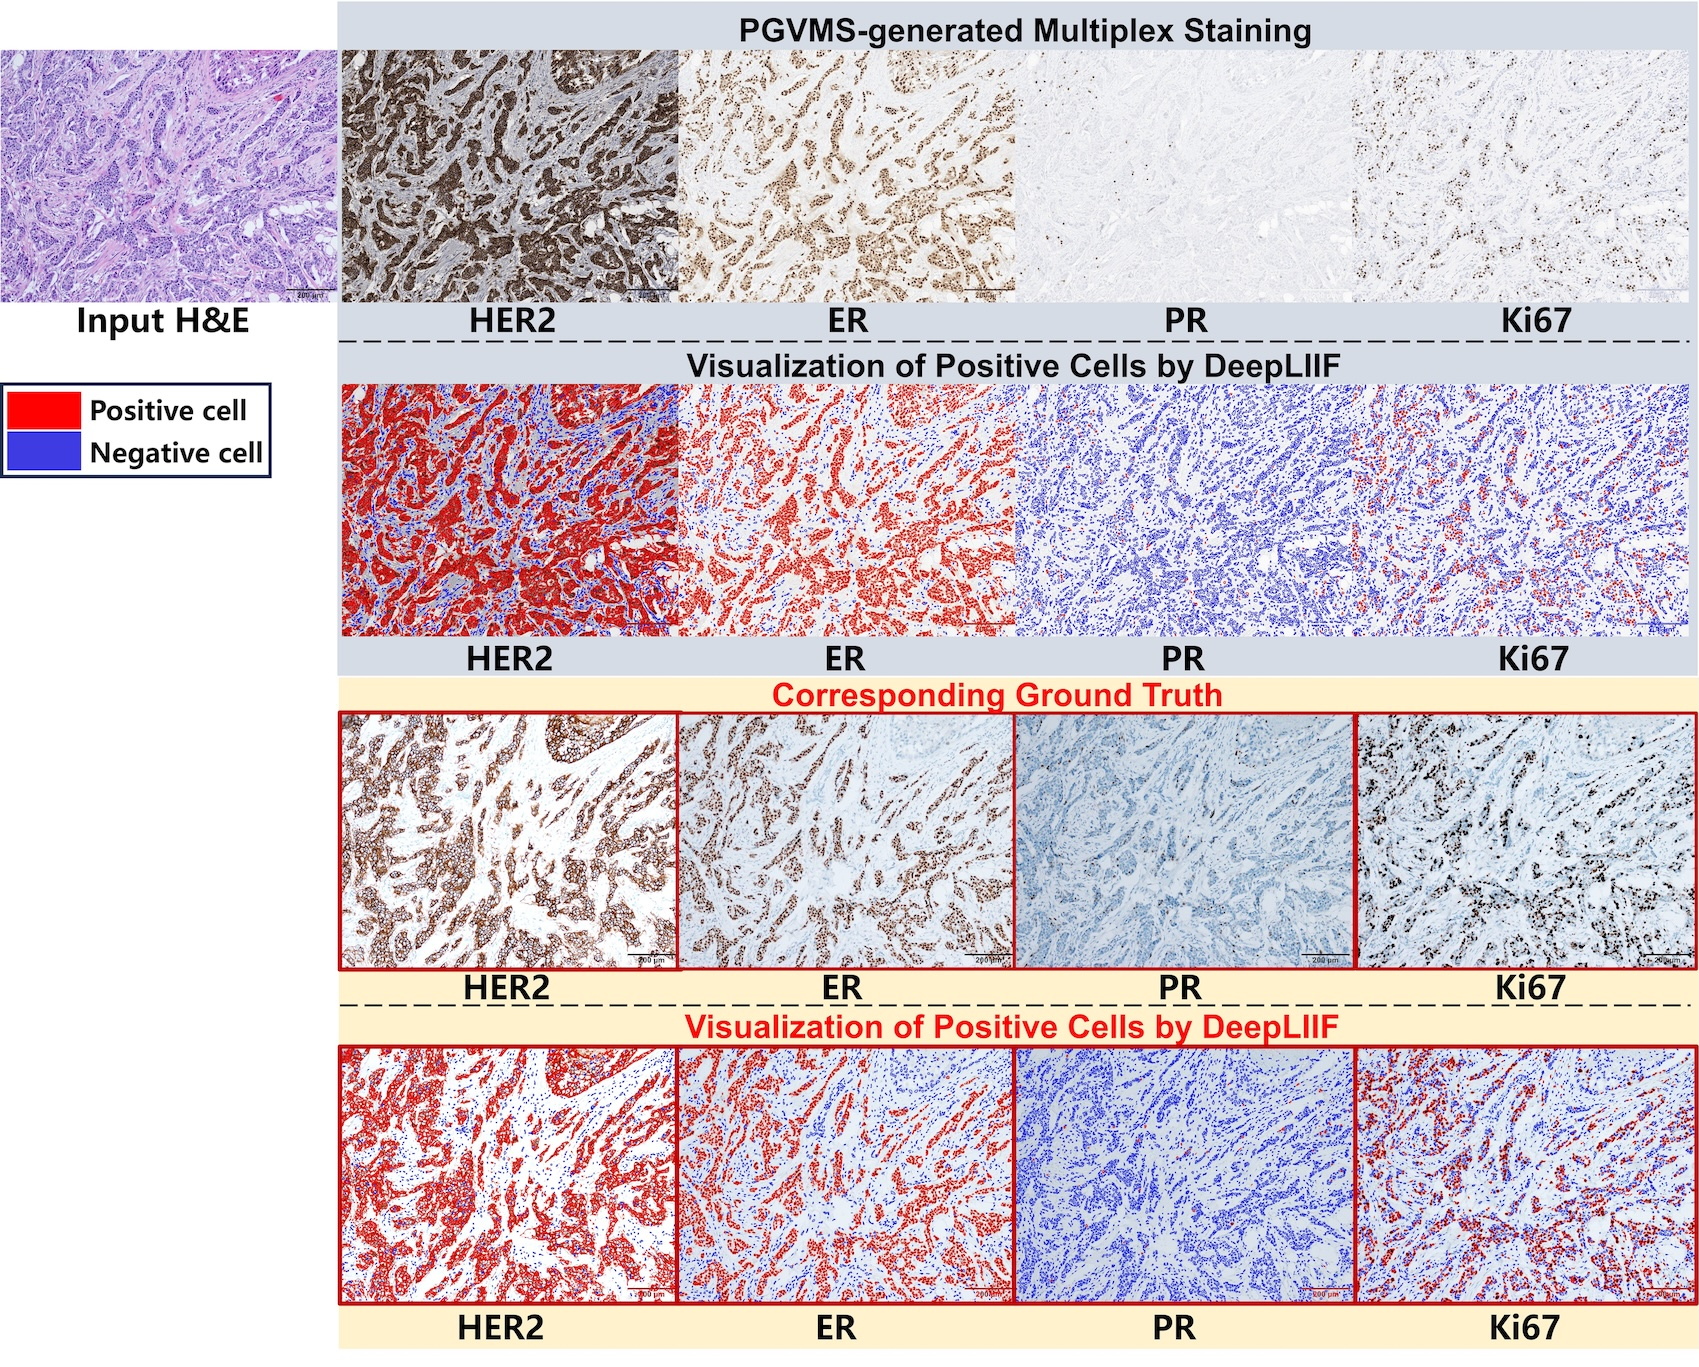
\includegraphics[width=\columnwidth,height=1\textheight,keepaspectratio]{image/qin12.jpg}
    \caption{\revision{Virtual IHC-stained image results on the clinical dataset, showing four stains (HER2, ER, PR, Ki-67) and positive cell visualization obtained using DeepLIIF. The first column shows the input H\&E images. Images with a gray background represent PGVMS-generated multiplex stains along with their corresponding positive cell visualization, while images with an yellow background show the ground truth multiplex stains and the associated positive cell visualization.}}

    \label{qualitative_qin_bci_2}
\end{figure}


\begin{figure}[!htbp]
    \centering
    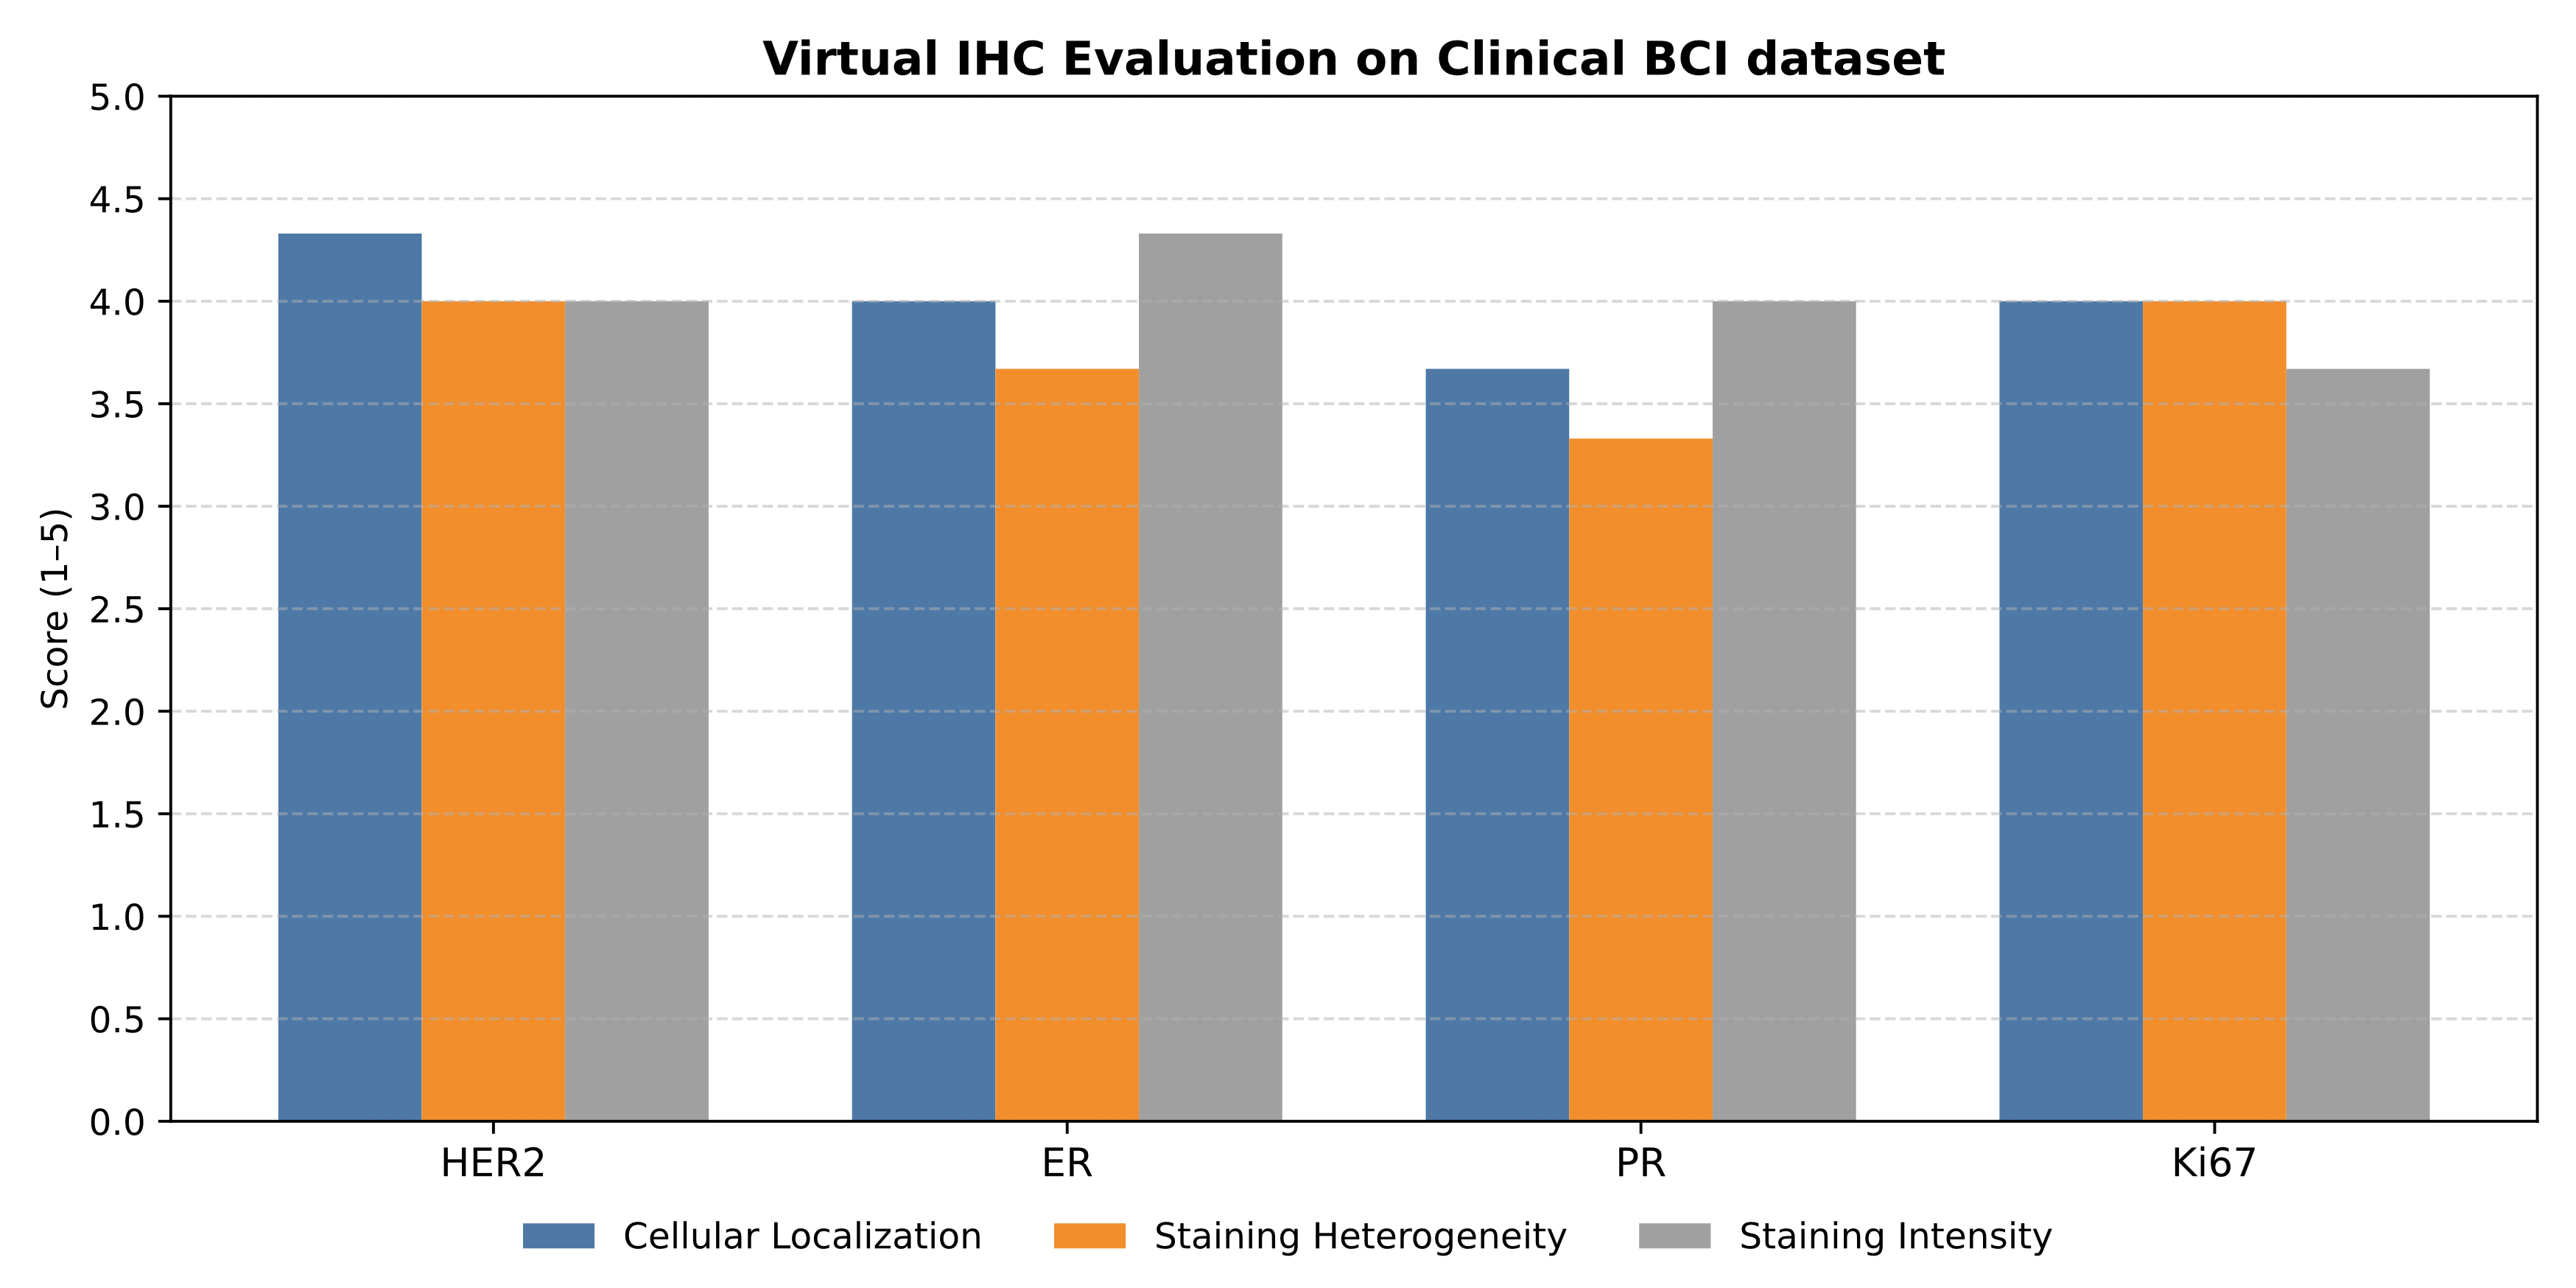
\includegraphics[width=\columnwidth,height=1\textheight,keepaspectratio]{image/qin13.png}
    \caption{{Virtual IHC-stained image results on the clinical dataset.  PGVMS preserves accurate cellular localization and realistic staining intensity across different biomarker.}}
    \label{qualitative_qin_bci_3}
\end{figure}


{
As shown in Figure~\ref{qualitative_qin_bci_2}, our method robustly generates all four stains for previously unseen patients, 
demonstrating strong generalization at the patient level. An experienced pathologist evaluated the virtual IHC-stained images on a five-point scale (1–5) across three criteria: cellular localization, staining heterogeneity, and staining intensity, as shown in Figure~\ref{qualitative_qin_bci_3}.
These results indicate that PGVMS can effectively handle variations in tissue morphology and staining patterns, supporting its potential applicability in diverse clinical scenarios.
}

\subsection{Cross-Organ and Cross-Cancer Generalization of PGVMS}

{
To evaluate the generalization ability of our PGVMS framework across different organs, cancer types, and IHC biomarkers, 
we conducted experiments on multiple independent clinical datasets, covering colon, liver, nasopharyngeal, and head-and-neck cancers. 
}
{
For each organ, we collect representative ROIs containing key biomarkers (e.g., Ki-67 for colorectal, HepPar1 for liver,  EBER and CK for nasopharyngeal carcinoma, PD-L1 for head and neck).
}

% (e.g., HepPar1 for liver, PD-L1 for head and neck, Ki-67 for colorectal, EBER and CK for nasopharyngeal carcinoma)

% \subsubsection{Clinical Breast Cancer Dataset} 
% A small subset of a private clinical breast cancer dataset contains all four stains (HER2, ER, PR, Ki-67).  
% Each image was cropped from WSIs into patches of size $4096 \times 3072$. As shown in Figure~\ref{qualitative_qin_bci_2}, PGVMS robustly generates all four stains for previously unseen patients, demonstrating good generalization at the patient level.

% \begin{figure}[!htbp]
% \centerline{\includegraphics[width=\columnwidth,height=0.9\textheight,keepaspectratio]{QIN_BCI_3.jpg}}
% \caption{Virtual IHC-stained image results on the clinical breast cancer dataset, showing HER2, ER, PR, Ki-67 stains and positive cell visualization from DeepLIIF.}
% \label{qualitative_qin_bci_2}
% \end{figure}

\subsubsection{Clinical Colon Cancer Dataset} 
{
We collected 69 ROIs from WSIs, each with paired upper and lower sections stained with H\&E and Ki-67 IHC.  
ROIs were cropped to $4096 \times 3072$ patches, and transfer learning for 10 epochs was applied.
}

\begin{figure}[!htbp]
\centerline{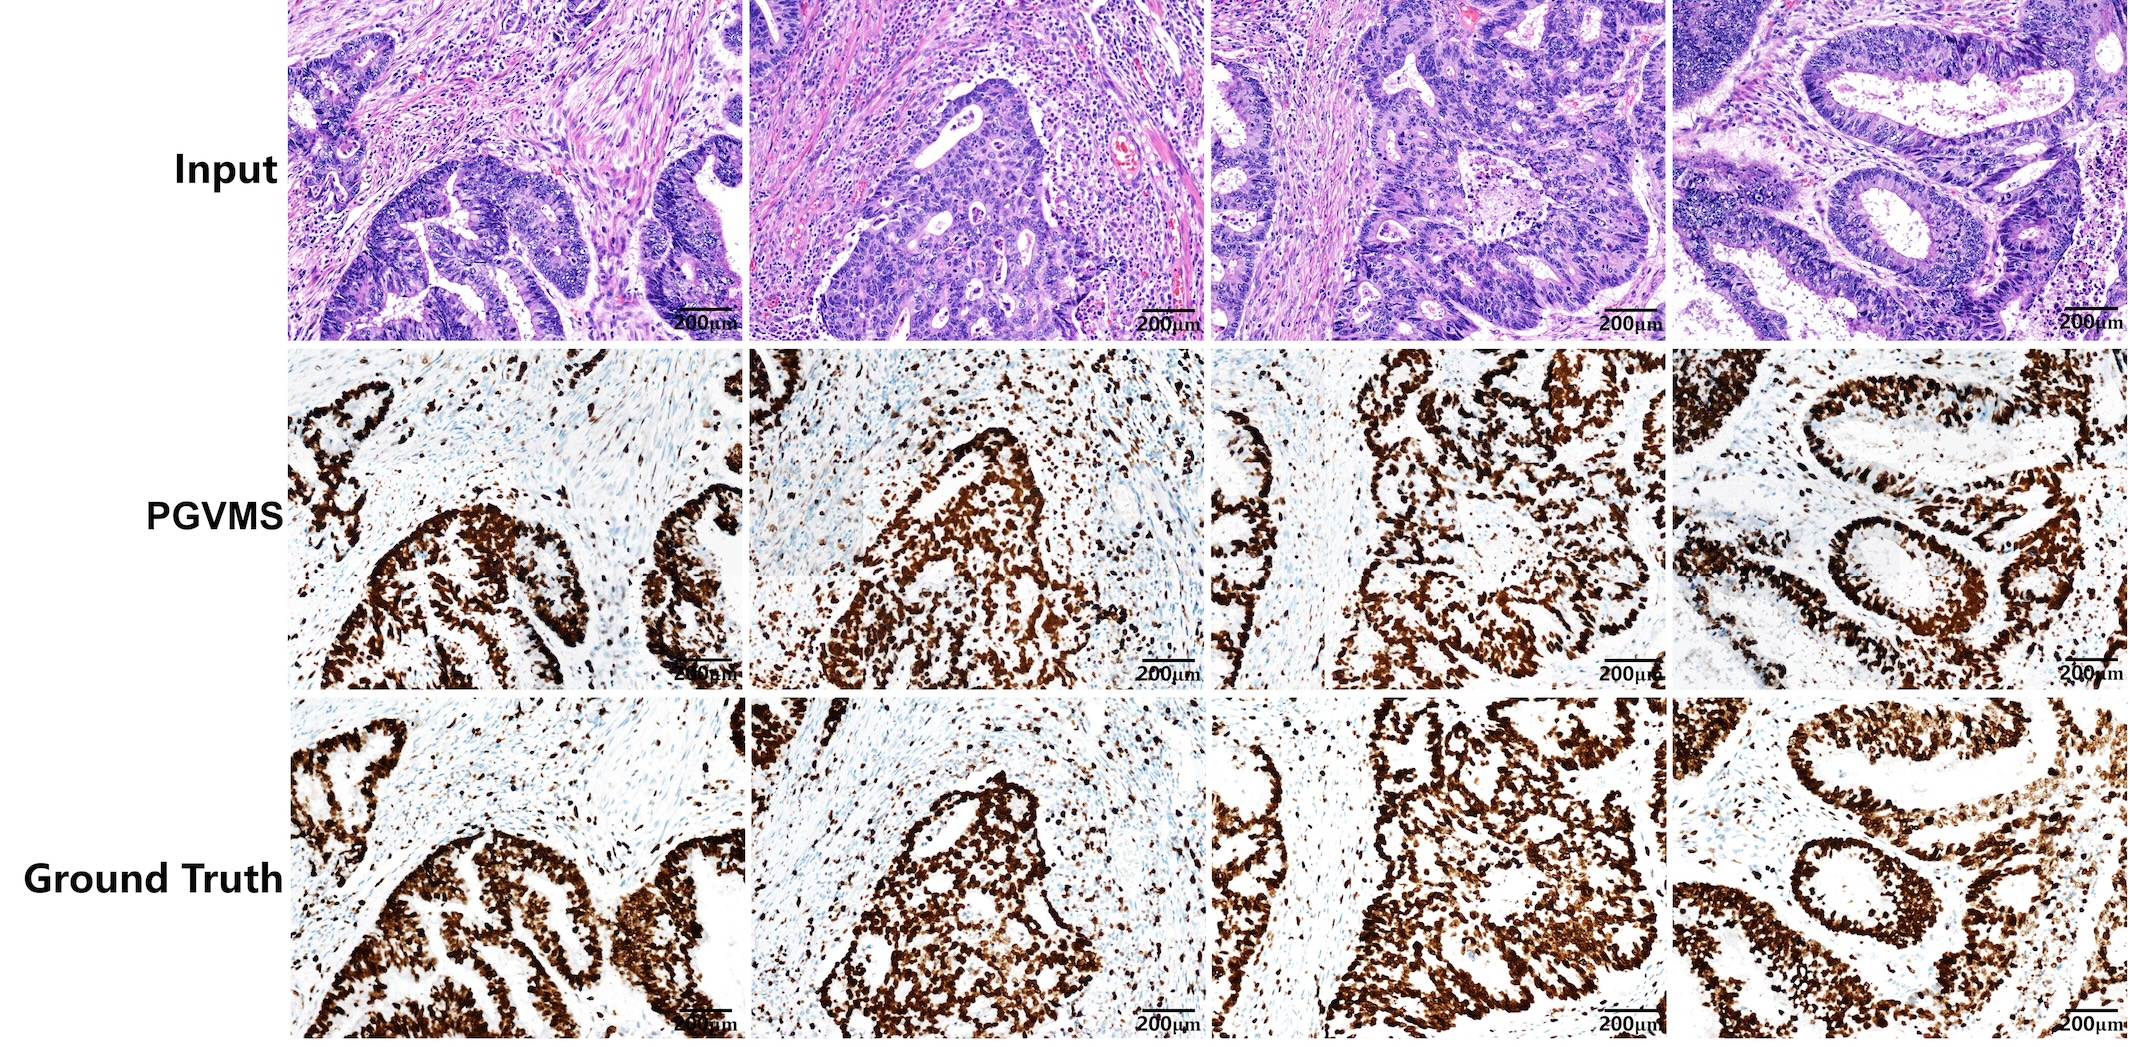
\includegraphics[width=\columnwidth,height=1\textheight,keepaspectratio]{image/qin14.jpg}}
\caption{{Virtual Ki-67-stained image results on the clinical colon cancer dataset.}}
\label{qualitative_colon_1}
\end{figure}

{
PGVMS synthesizes Ki-67-stained images (Fig. \ref{qualitative_colon_1}) with clear nuclear localization and structural fidelity comparable to the reference IHC slides.}

\subsubsection{Clinical Hepatocellular Carcinoma (HCC) Dataset} 
{
38 ROIs with paired H\&E and HepPar1 IHC sections were cropped to $4096 \times 3072$, and transfer learning was applied for 10 epochs.
}


\begin{figure}[!htbp]
\centerline{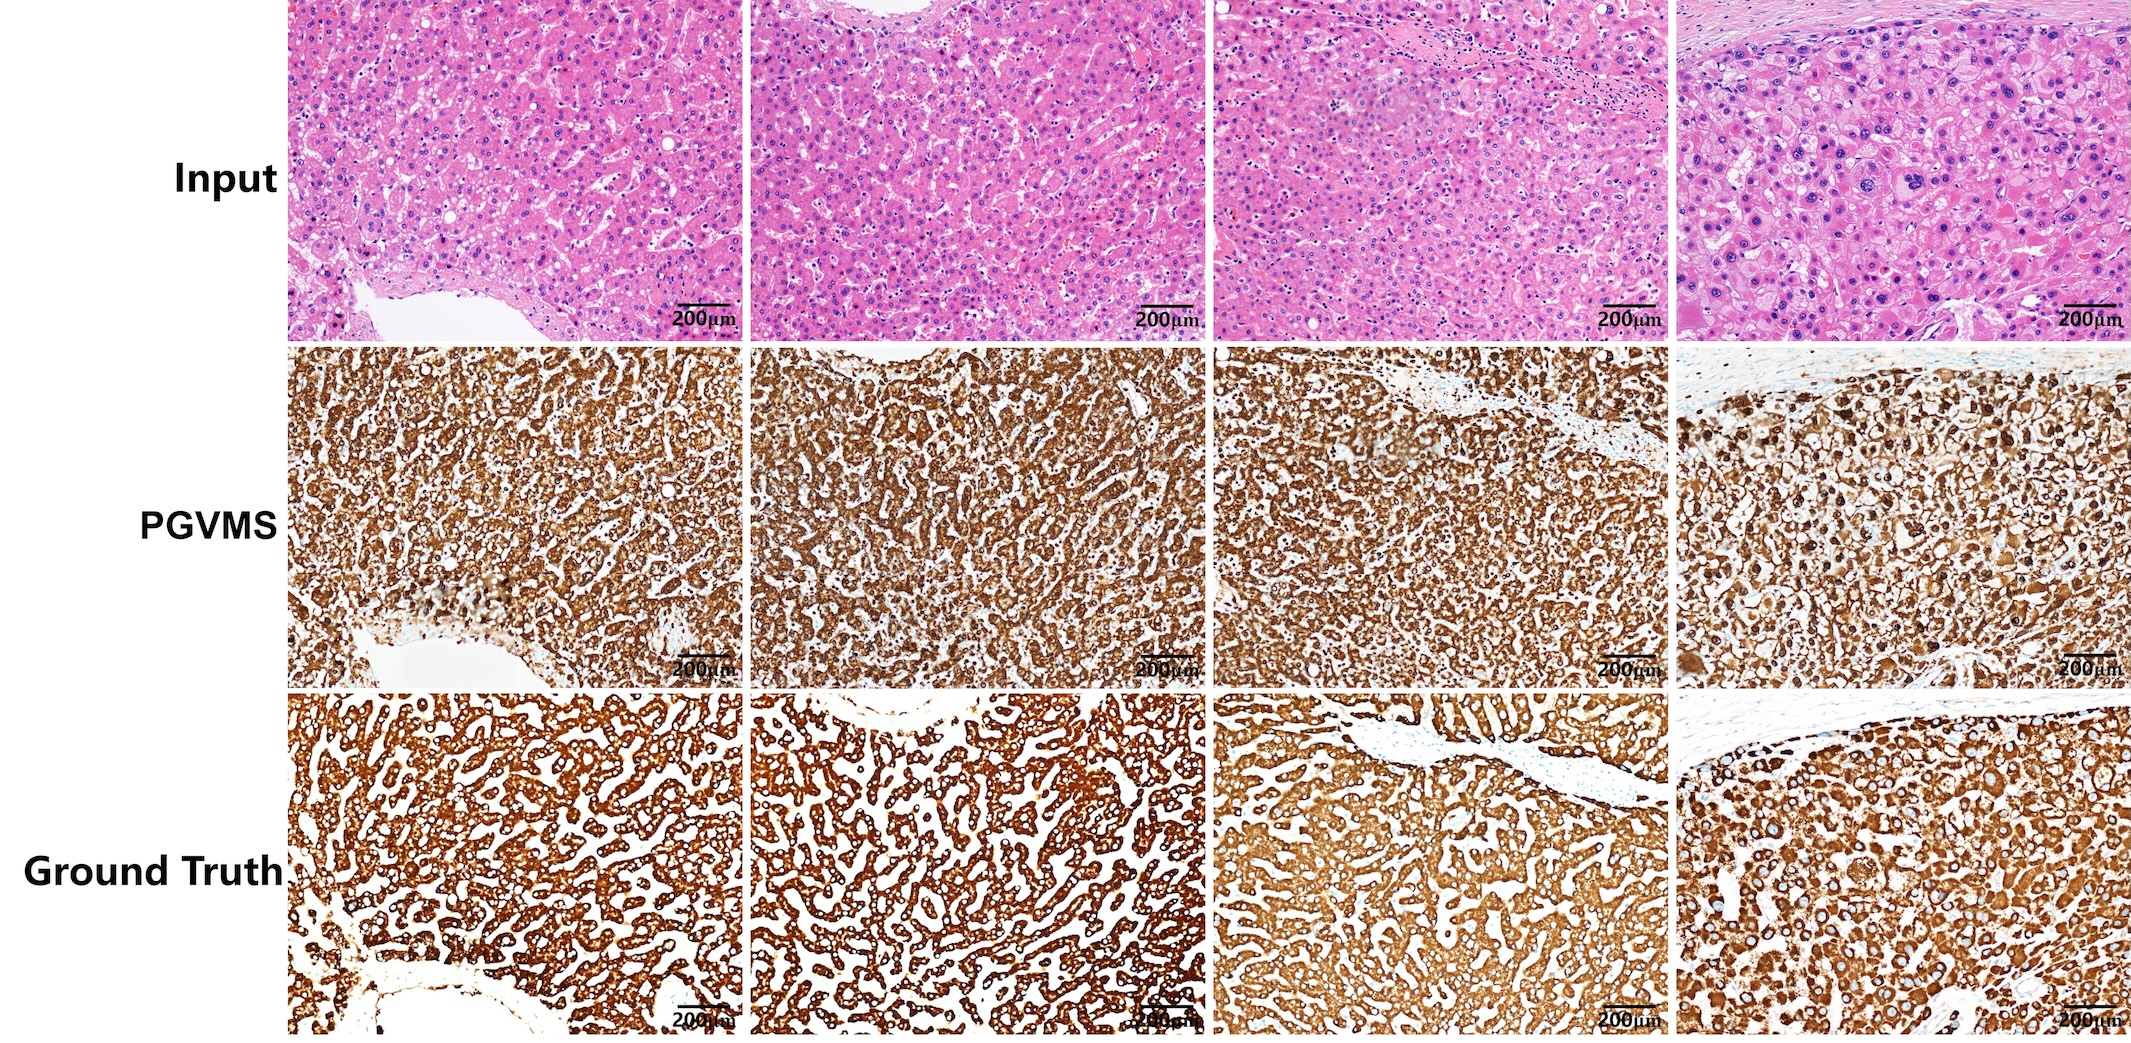
\includegraphics[width=\columnwidth,height=1\textheight,keepaspectratio]{image/qin15.jpg}}
\caption{{Virtual HepPar1 IHC-stained image results on the clinical HCC dataset.}}
\label{qualitative_liver_1}
\end{figure}

{
PGVMS (Fig. \ref{qualitative_liver_1}) preserves hepatocyte morphology and cytoplasmic staining patterns consistent with ground-truth slides.
}

\subsubsection{Clinical Nasopharyngeal Carcinoma (NPC) Dataset} 
{
57 ROIs were collected: 46 cases with CK and EBER stains, 11 cases with CK only. ROIs were cropped to $4096 \times 3072$, and the pretrained model was fine-tuned for 10 epochs.
}

\begin{figure}[!htbp]
\centerline{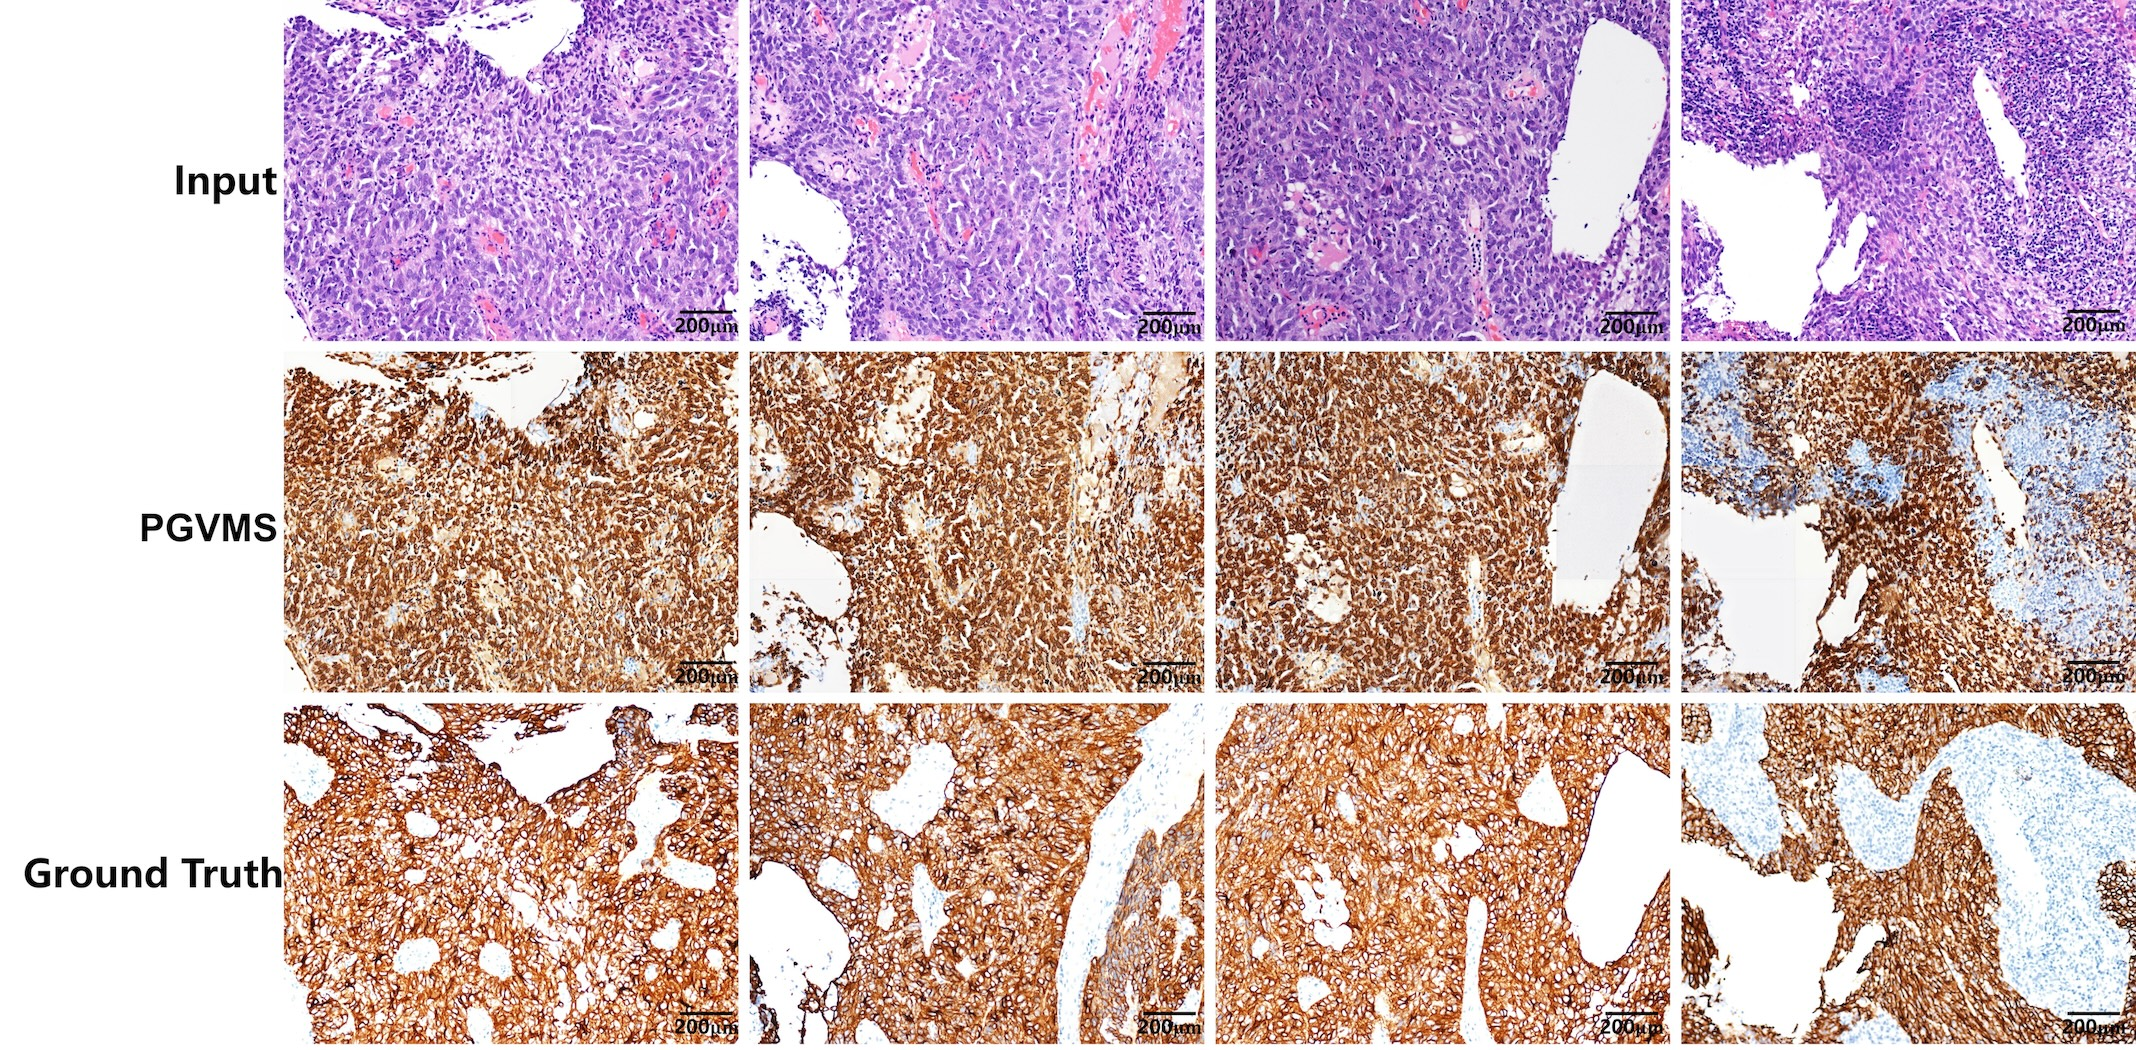
\includegraphics[width=\columnwidth,height=1\textheight,keepaspectratio]{image/qin16.jpg}}
\caption{{Virtual CK-stained image results on the clinical NPC dataset.}}
\label{qualitative_CK_1}
\end{figure}

\begin{figure}[!htbp]
\centerline{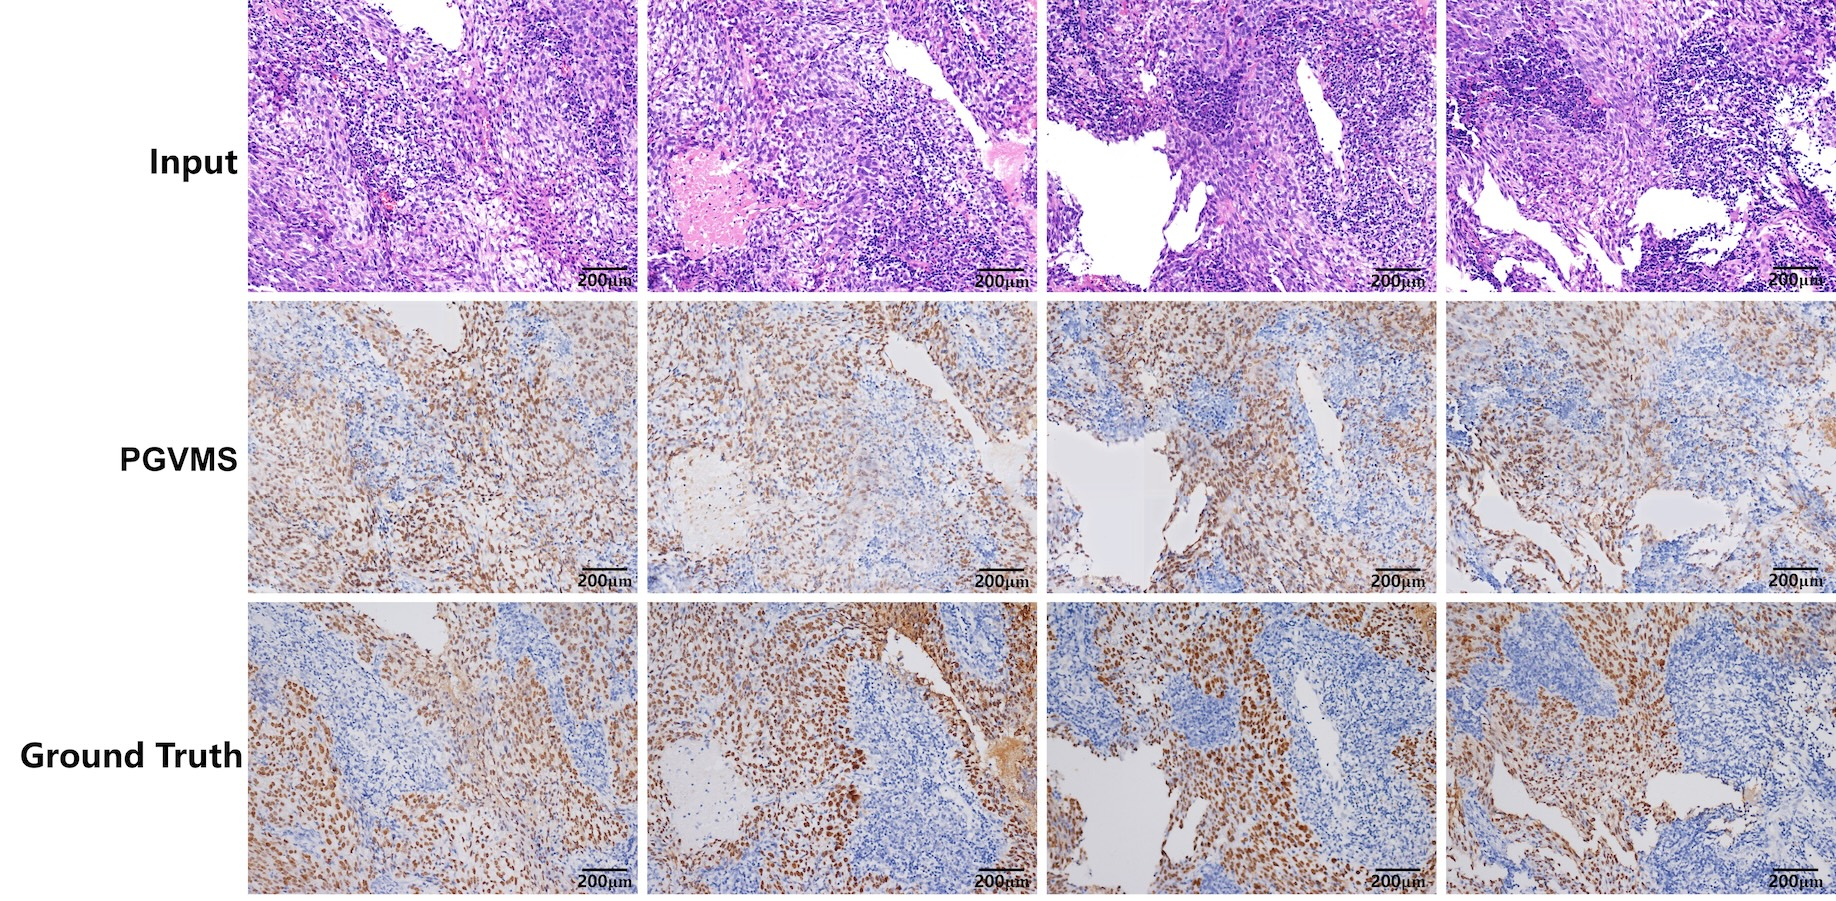
\includegraphics[width=\columnwidth,height=1\textheight,keepaspectratio]{image/qin17.jpg}}
\caption{{Virtual EBER-stained image results on the clinical NPC dataset.}}
\label{qualitative_EBER_1}
\end{figure}

{
PGVMS synthesizes CK and EBER stains (Fig. \ref{qualitative_CK_1} and Fig. \ref{qualitative_EBER_1}) with realistic contrast and structural fidelity comparable to reference slides.
}


\subsubsection{Clinical Head and Neck Squamous Cell Carcinoma (HNSCC) Datasets} 
{
17 ROIs with paired H\&E and PD-L1 IHC sections were cropped to $4096 \times 3072$ patches, and the model was fine-tuned for 10 epochs.
}

\begin{figure}[!htbp]
\centerline{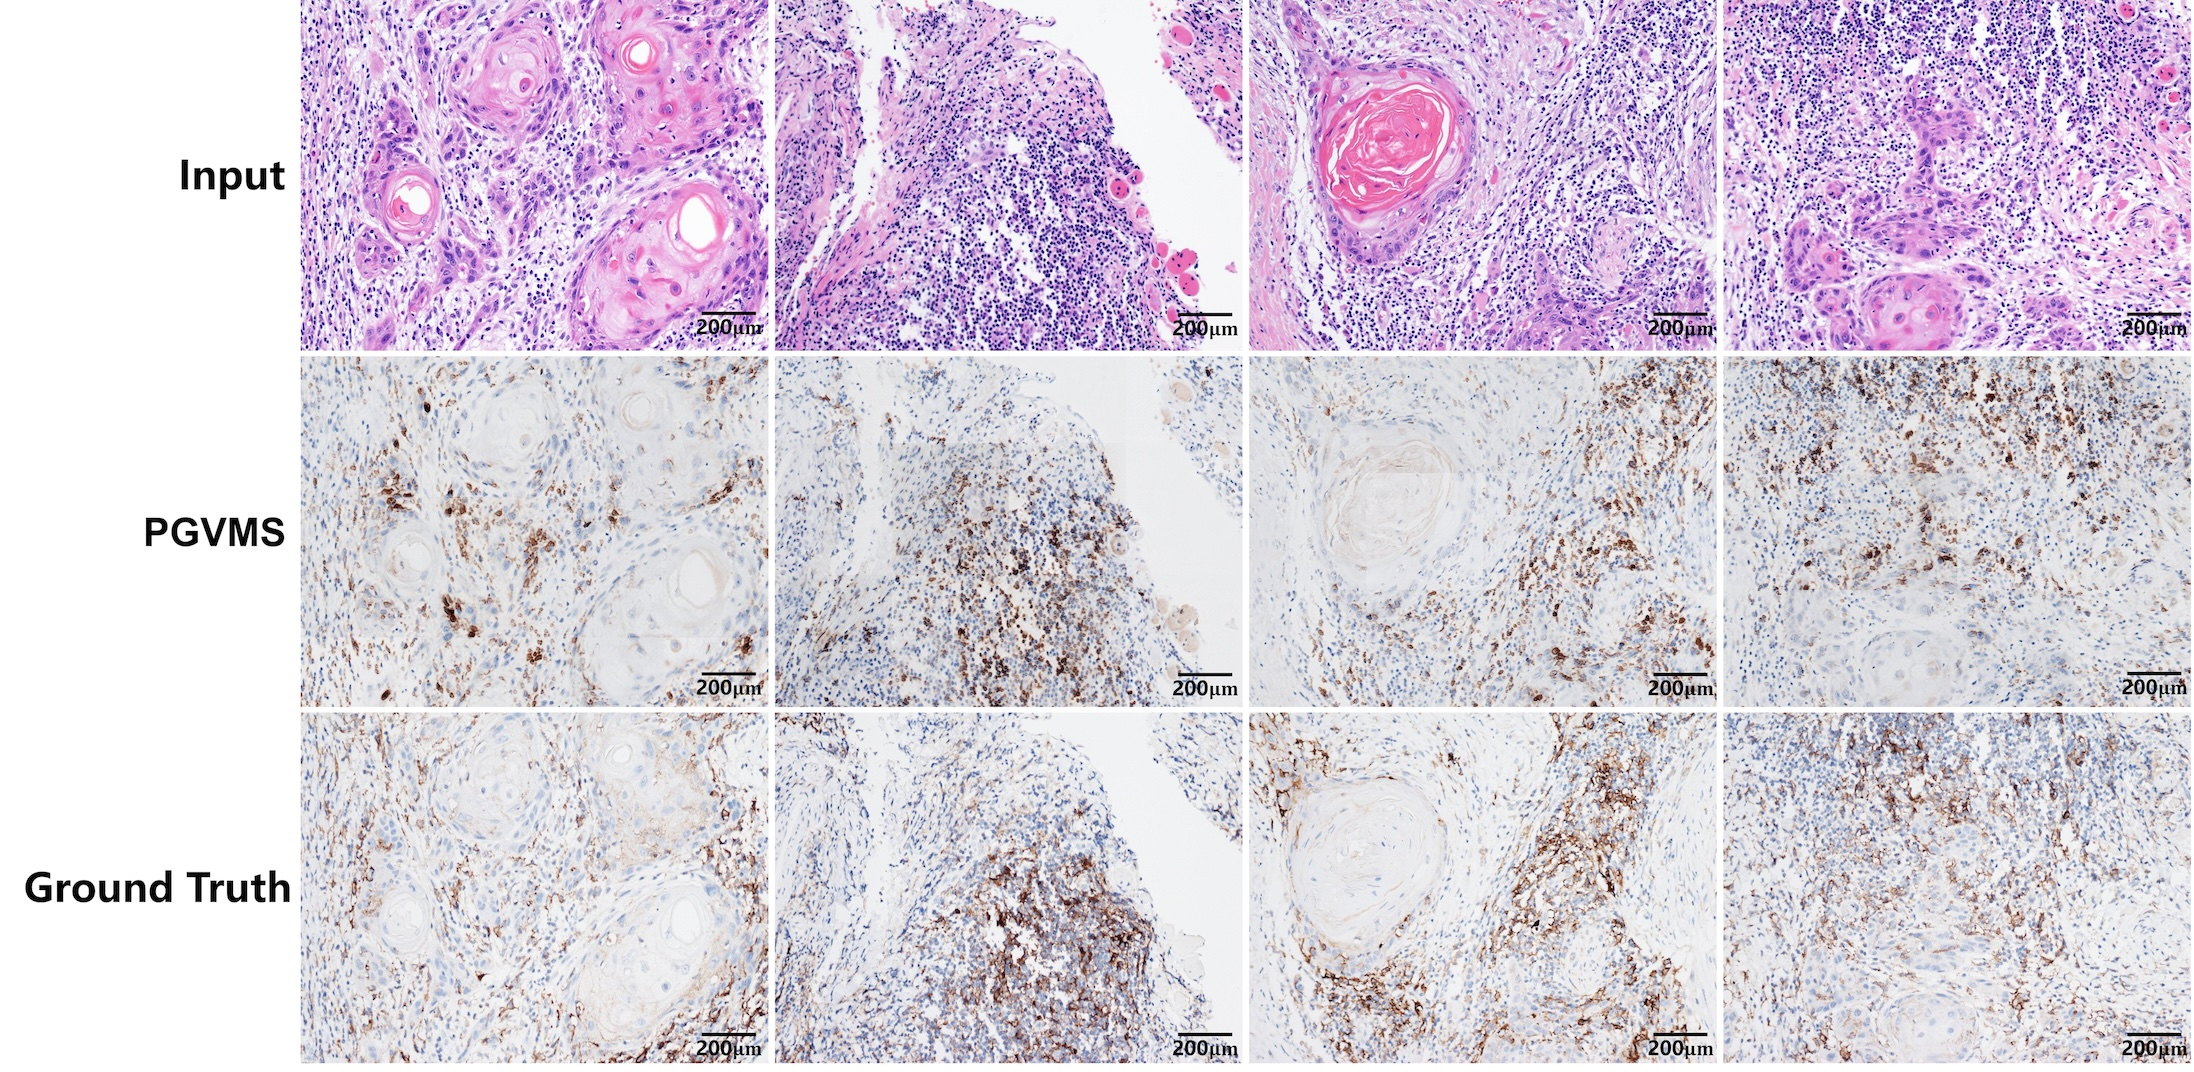
\includegraphics[width=\columnwidth,height=1\textheight,keepaspectratio]{image/qin18.jpg}}
\caption{{Virtual PD-L1 IHC-stained image results on the clinical HNSCC dataset.}}
\label{qualitative_hnscc_1}
\end{figure}

{
PGVMS generates virtual PD-L1-stained images (Fig. \ref{qualitative_hnscc_1}) exhibiting realistic membrane staining and expression intensity consistent with reference slides.
}

\subsubsection{Pathologist Evaluation}
{Experienced pathologist was asked to evaluate the virtual IHC-stained images on a five-point scale (1–5) across three aspects: 
cellular localization, {staining heterogeneity}, and {staining intensity} in Fig.~\ref{qualitative_organ}. 
}
% {
% As illustrated in Fig.~\ref{qualitative_organ}, the virtual IHC-stained images achieve consistently high quality across all criteria, 
% with mean scores exceeding 3.0 and often approaching 4.0 or higher. 
% }
\begin{figure}[!htbp] \centerline{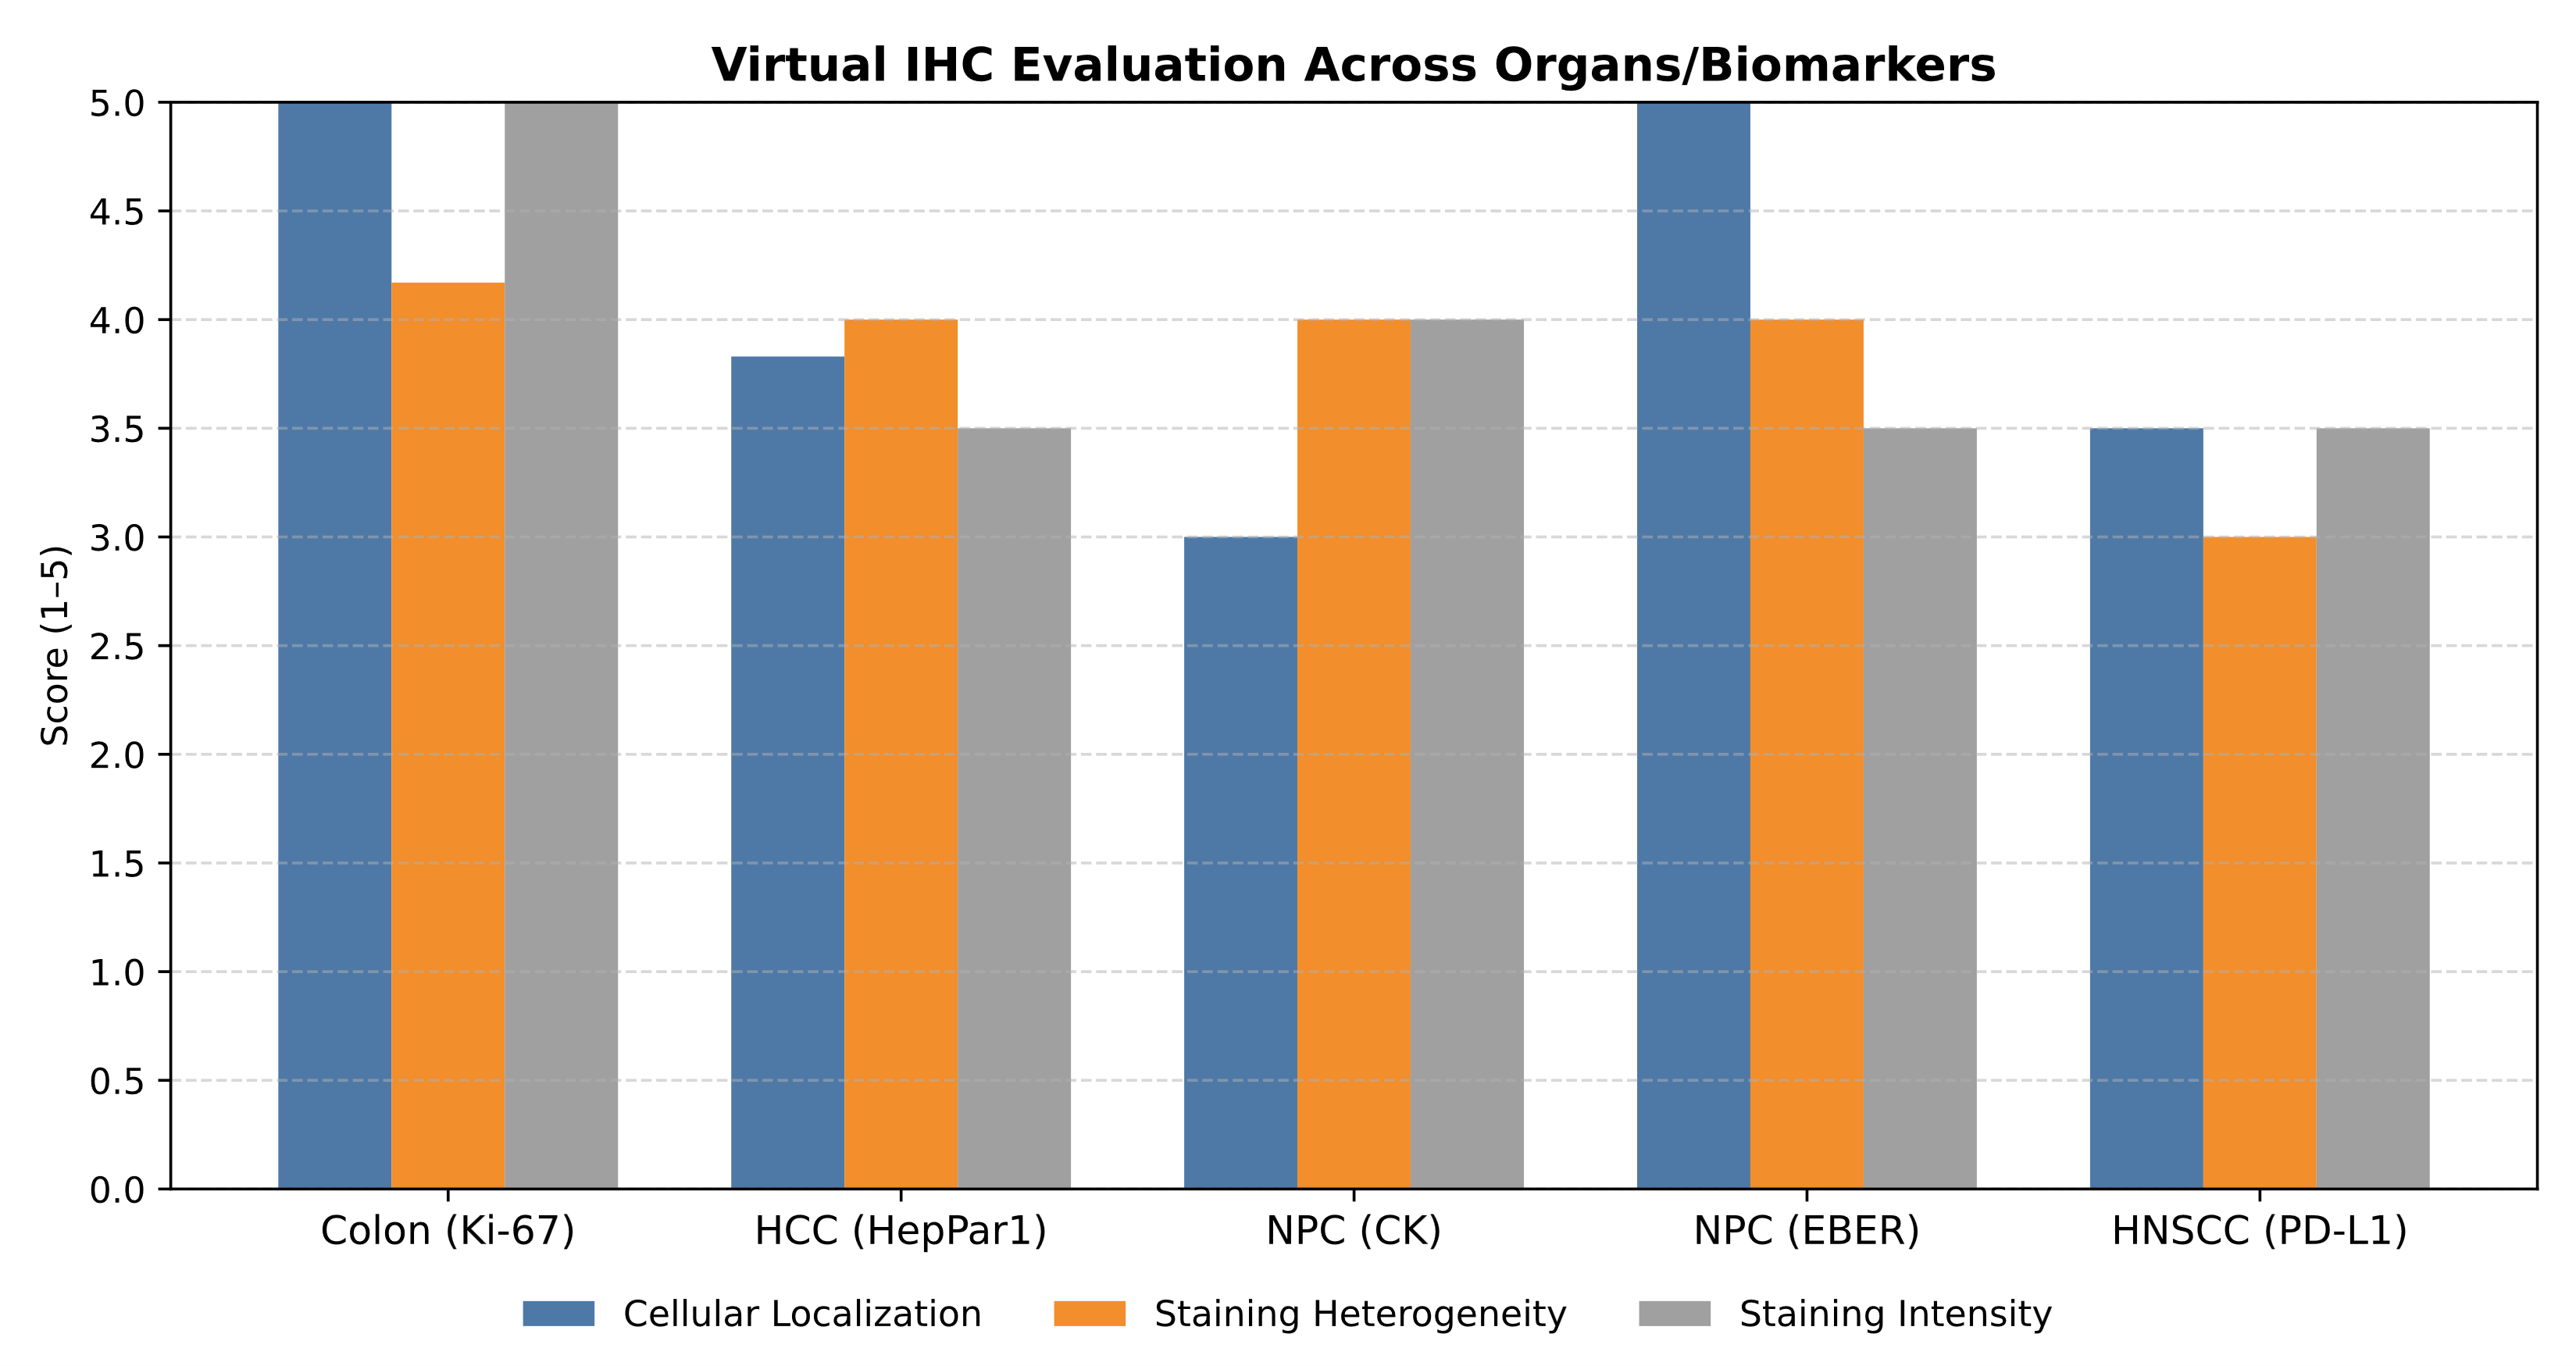
\includegraphics[width=\columnwidth]{image/qin19.png}} 
\caption{{Representative cross-organ virtual IHC staining results on liver, head-and-neck, colorectal, and nasopharyngeal samples. 
PGVMS preserves accurate cellular localization and realistic staining intensity across different biomarkers.}}
\label{qualitative_organ} 
\end{figure}

{
Specifically, Ki-67 and EBER achieve the highest overall ratings, demonstrating accurate nuclear localization and strong contrast between positive and negative regions. 
HepPar1 also performs well, showing clear cytoplasmic staining with minimal artefacts. 
PD-L1 and CK exhibit stable results across all three aspects, confirming the robustness of PGVMS on diverse tissue structures and staining patterns. 
Across all datasets, PGVMS demonstrates strong cross-organ and cross-cancer generalization, accurately synthesizing multiple IHC stains from H\&E images, maintaining morphological fidelity, and preserving biologically meaningful staining patterns suitable for diverse clinical scenarios.
}
% \subsection{Exploration of Metric Upper Bounds under Spatial Misalignment}
%, indicating that the model is lightweight and computationally affordable for large-scale deployment
% To quantitatively evaluate the robustness of our model under realistic spatial inconsistencies, 
% we developed a \textbf{controlled non-affine deformation simulator} that synthetically introduces inter-layer misalignment into IHC images. 
% This simulation framework allows systematic analysis of metric sensitivity and model performance degradation under varying distortion severities.  

% Following recent misalignment-resilience studies~\cite{ma2025generative}, 
% we apply patch-wise random displacements to construct a continuous deformation field:
% \begin{equation}
% \mathbf{x}' = \mathbf{x} + \Delta\mathbf{x}_{\text{local}} + \Delta\mathbf{x}_{\text{global}},
% \end{equation}
% where $\Delta\mathbf{x}_{\text{local}}$ denotes localized non-linear perturbations emulating fine-scale tissue deformation, 
% and $\Delta\mathbf{x}_{\text{global}}$ represents a global translational offset mimicking serial-section layer shifts. 
% By tuning the displacement magnitudes, we generate varying levels of misalignment severity to approximate realistic inter-layer distortions observed in practical histopathology workflows.

% Non-rigid deformation magnitudes were chosen to be physiologically and practically motivated. 
% WSIs in our study were acquired at 40× scanning resolution ($\approx$0.25~$\mu$m/pixel), allowing conversion of pixel displacements to physical units. 
% We define three misalignment regimes:
% \begin{itemize}
%   \item \textbf{Mild:} 5–10 px ($\approx$1.25–2.5~$\mu$m), representing small local deviations well below typical nuclear diameters.
%   \item \textbf{Moderate:} 10–15 px ($\approx$2.5–3.75~$\mu$m), approaching a sizable fraction of nuclear diameters and producing visibly displaced cellular regions.
%   \item \textbf{Severe:} 20–30 px ($\approx$5–7.5~$\mu$m), on the order of typical nucleus diameters and sufficient to disrupt pixel-level cell correspondence.
% \end{itemize}

% These ranges align with empirical observations: typical mammalian nuclei measure $\approx$5–10~$\mu$m, 
% and prior registration studies report median target registration errors (TRE) spanning the ~$\mu$m scale (restained pairs $\approx$0.9–2.2~$\mu$m; consecutive pairs often larger, up to tens of ~$\mu$m)~\cite{lotz2023comparison, gatenbee2023virtual}. 
% Hence, our mild/moderate/severe regimes map to observed TRE regimes, enabling evaluation of model robustness from near-nucleus-level alignment to challenging scenarios.

% To approximate empirical prevalence in practice, we constructed a mixed misalignment set by sampling mild/moderate/severe deformations with a 6:3:1 ratio, 
% reflecting that most serial sections exhibit small residual misalignment, fewer show moderate non-linear deformations, 
% and only a minority are severely distorted (e.g., due to folds, tears, or scanning artefacts). 
% Per-level results are also reported to demonstrate that conclusions do not rely critically on mixture weights.

% Based on these simulated misalignment experiments, we can estimate the \textit{upper bound} of existing evaluation metrics under realistic registration noise conditions. 
% Tables~\ref{tab:mist_Upper_bound} and~\ref{tab:IHC4BC_Upper_bound} summarize the estimated upper bounds for the \textbf{MIST} and \textbf{IHC4BC} datasets, respectively.



% This analysis establishes a practical \textit{upper bound} for commonly used evaluation metrics under realistic registration noise, 
% helping to contextualize the observed performance of PGVMS and other virtual staining methods.

% \begin{table}[ht]
%   \centering
%   \setlength{\tabcolsep}{2pt}
%   \renewcommand{\arraystretch}{1.0}
%   \caption{Estimated upper bound of evaluation metrics on MIST and IHC4BC datasets.}
%   \label{tab:upper_bound_summary}
%   \resizebox{\columnwidth}{!}{
%     \begin{tabular}{c|cc|cc|cc}
%       \Xhline{1.5pt} 
%       \multirow{2}{*}{Dataset} 
%       & \multicolumn{2}{c|}{Quality} & \multicolumn{2}{c|}{Pathology} & \multicolumn{2}{c}{Perception} \\
%       \cline{2-7}
%       & PSNR$\uparrow$ & SSIM$\uparrow$ & IOD$_{\times10^7}$ & Pearson-R$\uparrow$ & FID$\downarrow$ & DISTS$\downarrow$ \\
%       \hline
%       MIST & 19.1853 & 0.3791 & -0.1045 & 0.9999 & 18.3117 & 0.0738 \\
%       IHC4BC & 21.5494 & 0.4853 & -0.0557 & 0.9995 & 17.1023 & 0.0967 \\
%       \Xhline{1.5pt} 
%     \end{tabular}
%   }
% \end{table}
% \begin{table}[h!]
% \centering
% \caption{Average PSNR values for different methods and Gaussian blur kernels.}
% \label{tab:psnr_results}
% \begin{tabular}{c|cccc}
% \Xhline{1.5pt} 
% \textbf{PSNR} & \textbf{No Blur} & \textbf{Kernel 3x3} & \textbf{Kernel 5x5} & \textbf{Kernel 7x7} \\
% \hline
% CycleGAN & 13.3060 & 13.4611 & 13.5518 & 13.6656 \\
% Pix2Pix & 14.3445 & 14.4810 & 14.5597 & 14.6546 \\
% CUT & 14.2183 & 14.3632 & 14.4553 & 14.5692 \\
% ASP & 14.2746 & 14.4244 & 14.5189 & 14.6330 \\
% Pyramid & 14.3320 & 14.4816 & 14.5731 & 14.6877 \\
% TDKStain & 14.6360 & 14.7828 & 14.8702 & 14.9784 \\
% PSPStain & 14.4773 & 14.6160 & 14.6973 & 14.8003 \\
% PGVMS & 14.3421 & 14.5022 & 14.6046 & 14.7304 \\
% \hline
% Label &- &36.4453 & 33.0669 &	30.3883\\
% \Xhline{1.5pt} 
% \end{tabular}
% \end{table}

% \begin{table}[h!]
% \centering
% \caption{Average SSIM values for different methods and Gaussian blur kernels.}
% \label{tab:ssim_results}
% \begin{tabular}{c|cccc}
% \Xhline{1.5pt} 
% \textbf{SSIM} & \textbf{No Blur} & \textbf{Kernel 3x3} & \textbf{Kernel 5x5} & \textbf{Kernel 7x7} \\
% \hline
% CycleGAN & 0.2000 & 0.2264 & 0.2401 & 0.2561 \\
% Pix2Pix & 0.2143 & 0.2407 & 0.2558 & 0.2726 \\
% CUT & 0.2047 & 0.2318 & 0.2466 & 0.2633 \\
% ASP & 0.2144 & 0.2406 & 0.2553 & 0.2719 \\
% Pyramid & 0.2137 & 0.2402 & 0.2554 & 0.2715 \\
% TDKStain & 0.2181 & 0.2427 & 0.2563 & 0.2718 \\
% PSPStain & 0.2206 & 0.2458 & 0.2605 & 0.2767 \\
% PGVMS & 0.2032 & 0.2298 & 0.2453 & 0.2624 \\
% \hline
% Label &- & 0.9627 & 0.9189 & 0.8530\\
% \Xhline{1.5pt} 
% \end{tabular}
% \end{table}


% \section{Guidelines for Manuscript Preparation}
% Do not change the template font sizes or line spacing to squeeze more text into a limited number of pages.
% The preferred font is 10-pt Times New Roman. Use italics for emphasis; do not underline words.

% Place your figures in the text as you expect them to appear in print. Further instructions
% on figure usage appear in Section VI. Although IEEE will do the final formatting of your paper,
% we expect you to approximate the final form appearance for all versions
% submitted to TMI via ScholarOne\textregistered to the extent possible.

% \subsection{Abbreviations and Acronyms}
% Define abbreviations and acronyms the first time they are used in the text, 
% even after they have already been defined in the abstract. Abbreviations 
% such as IEEE, SI, ac, and dc do not have to be defined. Abbreviations that 
% incorporate periods should not have spaces: write ``C.N.R.S.,'' not ``C. N. 
% R. S.'' Do not use abbreviations in the title unless they are unavoidable 
% (for example, ``IEEE'' in the title of this article).

% \subsection{Other Recommendations}
% Use one space after periods and colons. Hyphenate complex modifiers: 
% ``zero-field-cooled magnetization.'' Avoid dangling participles, such as, 
% ``Using \eqref{eq}, the potential was calculated.'' It is not clear who or what 
% used \eqref{eq}. Write instead, ``The potential was calculated by using \eqref{eq},'' or 
% ``Using \eqref{eq}, we calculated the potential.''

% Use a zero before decimal points: ``0.25,'' not ``.25.'' Use 
% ``cm$^{3}$,'' not ``cc.'' Indicate sample dimensions as ``0.1 cm 
% $\times $ 0.2 cm,'' not ``0.1 $\times $ 0.2 cm$^{2}$.'' The 
% abbreviation for ``seconds'' is ``s,'' not ``sec.'' Use 
% ``Wb/m$^{2}$'' or ``webers per square meter,'' not 
% ``webers/m$^{2}$.'' When expressing a range of values, write ``7 to 
% 9'' or ``7--9,'' not ``7$\sim $9.''

% A parenthetical statement at the end of a sentence is punctuated outside of 
% the closing parenthesis (like this). (A parenthetical sentence is punctuated 
% within the parentheses.) In American English, periods and commas are located within 
% quotation marks, like ``this period.'' Other punctuation is placed ``outside''! 
% Avoid contractions; for example, write ``do not'' instead of ``don't.'' The 
% serial comma is preferred: ``A, B, and C'' instead of ``A, B and C.''

% If you wish, you may write in the first person singular or plural form using
% the active voice (``I observed that $\ldots$'' or ``We observed that $\ldots$'' 
% instead of ``It was observed that $\ldots$''). Remember to check spelling. If 
% your native language is not English, please have a native English-speaking 
% colleague to carefully proofread your paper.

% \section{Math}
% \subsection{Equations}
% Number equations consecutively with equation numbers in parentheses flush 
% with the right margin, as appears in \eqref{eq}. Refer to ``\eqref{eq},'' not ``Eq. \eqref{eq}'' 
% or ``equation \eqref{eq},'' except at the beginning of a sentence: ``Equation \eqref{eq} 
% is $\ldots$ .'' To make your equations more 
% compact, you may use the solidus (~/~), the exp function, or appropriate 
% exponents. Use parentheses to avoid ambiguities in denominators. Punctuate 
% equations when they are part of a sentence, as in
% \begin{equation}E=mc^2.\label{eq}\end{equation}

% Be sure to define the symbols in your equation before the equation appears or
% immediately following. Italicize symbols ($T$ might refer 
% to temperature, but T is the unit tesla).

% \subsection{\LaTeX-Specific Advice}

% Use ``soft'' (e.g., \verb|\eqref{Eq}|) cross references instead
% of ``hard'' references (e.g., \verb|(1)|). This will make it possible
% to combine sections, add equations, or change the order of figures or
% citations without having to manually change equation references.

% Do not use the \verb|{eqnarray}| equation environment. Use
% \verb|{align}| or \verb|{IEEEeqnarray}| instead. The \verb|{eqnarray}|
% environment leaves unsightly spaces around relation symbols.

% Note that the \verb|{subequations}| environment in {\LaTeX}
% will increment the main equation counter even when there are no
% equation numbers displayed.

% {\BibTeX} only functions in conjunction with local .bib files. If you use {\BibTeX} to produce the
% bibliography you must attach the .bib files.

% {\LaTeX} can't read your mind. If you assign the same label to both a
% subsubsection and a table, you may find that Table I has been cross
% referenced as Table IV-B3. 

% {\LaTeX} does not have precognitive abilities. If you put a
% \verb|\label| command before the command that updates the counter it's
% supposed to be using, the label will pick up the last counter to be
% cross referenced instead. In particular, a \verb|\label| command
% should not go before the caption of a figure or a table.

% Do not use \verb|\nonumber| inside the \verb|{array}| environment. It
% will not stop equation numbers inside \verb|{array}| and it might stop a
% wanted equation number in the surrounding equation.

% If you are submitting your paper to a colorized journal, you can use
% the following two lines at the start of the article to ensure its
% appearance resembles the final copy:

% \smallskip\noindent
% \begin{small}
% \begin{tabular}{l}
% \verb+\+\texttt{documentclass[journal,twoside,web]\{ieeecolor\}}\\
% \verb+\+\texttt{usepackage\{\textit{Journal\_Name}\}}
% \end{tabular}
% \end{small}

% \section{Units}
% Use either SI (MKS) or CGS as primary units. (SI units are strongly 
% encouraged.) English units may be used as secondary units (in parentheses). 
% For example, write ``1 kg (2.2lb).'' An exception exists for when 
% English units are used as identifiers in commercial products, such as a ``3\textonehalf-in 
% disk drive.'' Avoid combining SI and CGS units, such as current in amperes 
% and magnetic field in oersteds. This often leads to confusion because 
% equations do not balance dimensionally. If you must use mixed units, clearly 
% state the units for each quantity in an equation.

% The SI unit for magnetic field strength $H$ is A/m. However, if you wish to use 
% units of T, either refer to magnetic flux density $B$ or magnetic field 
% strength symbolized as $\mu _{0}H$. Use the center dot to separate 
% compound units, e.g., ``A$\cdot $m$^{2}$.''

% \begin{figure}[!t]
% \centerline{\includegraphics[width=\columnwidth]{fig1.png}}
% \caption{Magnetization as a function of applied field.
% It is good practice to explain the significance of the figure in the caption.}
% \label{fig1}
% \end{figure}

% \section{Guidelines for Graphics Preparation and Submission}
% \label{sec:guidelines}

% \subsection{Types of Graphics}
% The following list outlines the different types of graphics published in 
% IEEE journals. They are categorized based on their construction, and use of 
% color~/~shades of gray:

% \subsubsection{Color/Grayscale figures}
% {Figures that are meant to appear in color, or shades of black/gray. Such 
% figures may include photographs, illustrations, multicolor graphs, and 
% flowcharts.}

% \subsubsection{Line Art figures}
% {Figures that are composed of only black lines and shapes. These figures 
% should have no shades or half-tones of gray, only black and white.}

% \subsubsection{Author photos}
% {Not allowed for papers in TMI.}

% \subsubsection{Tables}
% {Data charts which are typically black and white, but sometimes include 
% color.}

% \begin{table}
% \caption{Units for Magnetic Properties}
% \label{table}
% \setlength{\tabcolsep}{3pt}
% \begin{tabular}{|p{25pt}|p{75pt}|p{115pt}|}
% \hline
% Symbol& 
% Quantity& 
% Conversion from Gaussian and \par CGS EMU to SI $^{\mathrm{a}}$ \\
% \hline
% $\Phi $& 
% magnetic flux& 
% 1 Mx $\to  10^{-8}$ Wb $= 10^{-8}$ V$\cdot $s \\
% $B$& 
% magnetic flux density, \par magnetic induction& 
% 1 G $\to  10^{-4}$ T $= 10^{-4}$ Wb/m$^{2}$ \\
% $H$& 
% magnetic field strength& 
% 1 Oe $\to  10^{3}/(4\pi )$ A/m \\
% $m$& 
% magnetic moment& 
% 1 erg/G $=$ 1 emu \par $\to 10^{-3}$ A$\cdot $m$^{2} = 10^{-3}$ J/T \\
% $M$& 
% magnetization& 
% 1 erg/(G$\cdot $cm$^{3}) =$ 1 emu/cm$^{3}$ \par $\to 10^{3}$ A/m \\
% 4$\pi M$& 
% magnetization& 
% 1 G $\to  10^{3}/(4\pi )$ A/m \\
% $\sigma $& 
% specific magnetization& 
% 1 erg/(G$\cdot $g) $=$ 1 emu/g $\to $ 1 A$\cdot $m$^{2}$/kg \\
% $j$& 
% magnetic dipole \par moment& 
% 1 erg/G $=$ 1 emu \par $\to 4\pi \times  10^{-10}$ Wb$\cdot $m \\
% $J$& 
% magnetic polarization& 
% 1 erg/(G$\cdot $cm$^{3}) =$ 1 emu/cm$^{3}$ \par $\to 4\pi \times  10^{-4}$ T \\
% $\chi , \kappa $& 
% susceptibility& 
% 1 $\to  4\pi $ \\
% $\chi_{\rho }$& 
% mass susceptibility& 
% 1 cm$^{3}$/g $\to  4\pi \times  10^{-3}$ m$^{3}$/kg \\
% $\mu $& 
% permeability& 
% 1 $\to  4\pi \times  10^{-7}$ H/m \par $= 4\pi \times  10^{-7}$ Wb/(A$\cdot $m) \\
% $\mu_{r}$& 
% relative permeability& 
% $\mu \to \mu_{r}$ \\
% $w, W$& 
% energy density& 
% 1 erg/cm$^{3} \to  10^{-1}$ J/m$^{3}$ \\
% $N, D$& 
% demagnetizing factor& 
% 1 $\to  1/(4\pi )$ \\
% \hline
% \multicolumn{3}{p{251pt}}{Vertical lines are optional in tables. Statements that serve as captions for 
% the entire table do not need footnote letters. }\\
% \multicolumn{3}{p{251pt}}{$^{\mathrm{a}}$Gaussian units are the same as cg emu for magnetostatics; Mx 
% $=$ maxwell, G $=$ gauss, Oe $=$ oersted; Wb $=$ weber, V $=$ volt, s $=$ 
% second, T $=$ tesla, m $=$ meter, A $=$ ampere, J $=$ joule, kg $=$ 
% kilogram, H $=$ henry.}
% \end{tabular}
% \label{tab1}
% \end{table}

% \subsection{Multipart figures}
% Multipart figures are comprised of more than one sub-figure presented together.
% If a multipart figure is made up of multiple figure types (one part is lineart,
% and another is grayscale or color) the figure should meet the strictest applicable guidelines.

% \subsection{File Formats For Graphics}
% \label{formats}
% Format and save your graphics as one of the following approved file types:
% PostScript (.PS), Encapsulated PostScript (.EPS), Tagged Image File Format (.TIFF),
% Portable Document Format (.PDF), Portable Network Graphics (.PNG), or Metapost (.MPS).
% After the paper is accepted, any included graphics must be submitted alongside the final manuscript files.

% \subsection{Sizing of Graphics}
% Most charts, graphs, and tables are one column wide (3.5 inches~/~88 
% millimeters) or page wide (7.16 inches~/~181 millimeters). The maximum
% depth of a graphic is 8.5 inches (216 millimeters). When choosing the depth of a graphic,
% please allow space for a caption. Authors are allowed to size figures between column and
% page widths, but it is recommended not to size figures less than column width unless necessary. 

% \subsection{Resolution}
% The proper resolution of your figures will depend on the type of figure it 
% is as defined in the ``Types of Figures'' section. Author photographs, 
% color, and grayscale figures should be at least 300dpi. Lineart, including 
% tables should be a minimum of 600dpi.

% \subsection{Vector Art}
% While IEEE does accept and even recommends that authors submit artwork
% in vector format, it is our policy is to rasterize all figures for publication. This is done
% in order to preserve figures' integrity across multiple computer platforms.

% \subsection{Colorspace}
% The term colorspace refers to the entire sum of colors that can be 
% represented within a given medium. For our purposes, the three main colorspaces
% are grayscale, RGB (red/green/blue) and CMYK (cyan/magenta/yellow/black).
% RGB is generally used with on-screen graphics, whereas CMYK is used for printing purposes.

% All color figures should be generated in RGB or CMYK colorspace. Grayscale 
% images should be submitted in grayscale colorspace. Line art may be 
% provided in grayscale OR bitmap colorspace. Note that ``bitmap colorspace'' 
% and ``bitmap file format'' are not the same thing. When bitmap colorspace 
% is selected, .TIF/.TIFF are the recommended file formats.

% \subsection{Accepted Fonts Within Figures}
% When preparing your graphics IEEE suggests that you use of one of the 
% following Open Type fonts: Times New Roman, Helvetica, Arial, Cambria, and 
% Symbol. If you are supplying EPS, PS, or PDF files all fonts must be 
% embedded. Some fonts may only be native to your operating system; without 
% the fonts embedded, parts of the graphic may be distorted or missing.

% A safe option when finalizing your figures is to strip out the fonts before 
% you save the files, creating ``outline'' type. This converts fonts to 
% artwork that will appear uniformly on any screen.

% \subsection{Using Labels Within Figures}

% \subsubsection{Figure Axis labels}
% Figure axis labels are often a source of confusion. Use words rather than 
% symbols. As an example, write the quantity ``Magnetization,'' or 
% ``Magnetization M,'' not just ``M.'' Put units in parentheses. Do not label 
% axes only with units. As in Fig. 1, for example, write ``Magnetization 
% (A/m)'' or ``Magnetization (A$\cdot$m$^{-1}$),'' not just ``A/m.''
% Do not label axes with a ratio of quantities and units.
% For example, write ``Temperature (K),'' not ``Temperature/K.'' 

% Multipliers can be especially confusing. Write ``Magnetization (kA/m)'' or 
% ``Magnetization (10$^{3}$ A/m).'' Do not write ``Magnetization 
% (A/m)$\,\times\,$1000'' because the reader would not know whether the top 
% axis label in Fig. 1 meant 16000 A/m or 0.016 A/m. Figure labels should be 
% legible, approximately 8 to 10 point type.

% \subsubsection{Subfigure Labels in Multipart Figures and Tables}
% Multipart figures should be combined and labeled before final submission. 
% Labels should appear centered below each subfigure in 8 point Times New 
% Roman font in the format of (a) (b) (c).

% \subsection{Referencing a Figure or Table Within Your Paper}
% When referencing your figures and tables within your paper, use the 
% abbreviation ``Fig.'' even at the beginning of a sentence. Do not abbreviate 
% ``Table.'' Tables should be numbered with Roman numerals.

% \subsection{Submitting Your Graphics}
% Format your paper with the graphics included within the body of the text
% as you would expect to see the paper in print. Please do this at each stage of the review,
% from first submission to final files. For final files only, after the paper has been accepted
% for publication, figures should also be submitted individually in addition to the manuscript
% file using one of the approved file formats. Place a figure caption below each figure;
% place table titles above the tables. Do not include captions or borders in the uploaded figure files.

% \subsection{File Naming}
% Figures (line artwork or images) should be named starting with the 
% first 5 letters of the corresponding author's last name. The next characters in the 
% filename should be the number that represents the figure's sequential 
% location in the article. For example, in author ``Anderson's'' paper,
% the first three figures might be named ander1.tif, ander2.tif, and ander3.ps.

% Tables should contain only the body of the table (not the caption) and 
% should be named similarly to figures, except that `.t' is inserted 
% in-between the author's name and the table number. For example, author 
% Anderson's first three tables would be named ander.t1.tif, ander.t2.ps, ander.t3.eps.

% Author photographs or biographies are not permitted in IEEE TMI papers.

% \subsection{Checking Your Figures: The IEEE Graphics Analyzer}
% The IEEE Graphics Analyzer enables authors to pre-screen their graphics for 
% compliance with IEEE Transactions and Journals standards before submission. 
% The online tool, located at \underline{http://graphicsqc.ieee.org/},
% allows authors to upload their graphics in order to check that each file is the correct file format,
% resolution, size and colorspace; that no fonts are missing or corrupt;
% that figures are not compiled in layers or have transparency,
% and that they are named according to the IEEE Transactions and Journals naming convention.
% At the end of this automated process, authors are provided with 
% a detailed report on each graphic within the web applet, as well as by email.

% For more information on using the Graphics Analyzer or any other graphics 
% related topic, contact the IEEE Graphics Help Desk by e-mail at 
% graphics@ieee.org.

% \subsection{Color Processing/Printing in IEEE Journals}
% All IEEE Transactions, Journals, and Letters allow an author to publish 
% color figures on IEEE Xplore\textregistered\ at no charge, and automatically 
% convert them to grayscale for print versions. In most journals, figures and 
% tables may alternatively be printed in color if an author chooses to do so. 
% Please note that this service comes at an extra expense to the author. If 
% you intend to have print color graphics, include a note with your final 
% paper indicating which figures or tables you would like to be handled that way,
% and stating that you are willing to pay the additional fee.

% \section{Some Common Mistakes}
% The word ``data'' is plural, not singular. The subscript for the 
% permeability of vacuum $\mu _{0}$ is zero, not a lowercase letter 
% ``o.'' Use the word ``micrometer'' instead of ``micron.'' A graph within a graph is an 
% ``inset,'' not an ``insert.'' The word ``alternatively'' is preferred to the 
% word ``alternately'' (unless you really mean something that alternates). Use 
% the word ``whereas'' instead of ``while'' (unless you are referring to 
% simultaneous events). Do not use the word ``essentially'' to mean 
% ``approximately'' or ``effectively.'' Do not use the word ``issue'' as a 
% euphemism for ``problem.'' When compositions are not specified, separate 
% chemical symbols by en-dashes; for example, ``NiMn'' indicates the 
% intermetallic compound Ni$_{0.5}$Mn$_{0.5}$ whereas 
% ``Ni--Mn'' indicates an alloy of some composition 
% Ni$_{x}$Mn$_{1-x}$.

% Be aware of the different meanings of the homophones ``affect'' (usually a 
% verb) and ``effect'' (usually a noun), ``complement'' and ``compliment,'' 
% ``discreet'' and ``discrete,'' ``principal'' (e.g., ``principal 
% investigator'') and ``principle'' (e.g., ``principle of measurement''). Do 
% not confuse ``imply'' and ``infer.'' 

% Prefixes such as ``non,'' ``sub,'' ``micro,'' ``multi,'' and ``ultra'' are 
% not independent words; they should be joined to the words they modify, 
% usually without a hyphen. There is no period after the ``et'' in the Latin 
% abbreviation ``\emph{et al.}'' (it is also italicized). The abbreviation ``i.e.,'' means 
% ``that is,'' and the abbreviation ``e.g.,'' means ``for example'' (these 
% abbreviations are not italicized).

% A general IEEE styleguide is available at \underline{http://www.ieee.org/web/publications/authors/transjnl/index.ht}
% \discretionary{}{}{}\underline{ml}.



\section{Conclusion}
In this work, we present PGVMS, a comprehensive framework for pathological prompt-guided IHC virtual multiplex staining using only uniplex training data. Our three key innovations: (1) the pathological semantics-style guided  (PSSG) generator with CONCH integration, (2) protein-aware learning strategy (PALS) with focal optical density mapping and (3) prototype-consistent learning strategy (PCLS) collectively address the critical challenges of semantic preservation, molecular-level accuracy, and spatial alignment in stain transformation. \revision{Extensive validation on MIST, IHC4BC, and cross-organ clinical datasets demonstrates state-of-the-art performance, with our method outperforming existing generative approaches while requiring no additional annotations.} This work bridges a critical gap in computational pathology by evolving virtual staining from isolated single-task solutions to an integrated system supporting multiplex diagnosis via prompt-based control. 

{
Our method, through the PCLS module, performs particularly well on clustered IHC patterns. However, biomarkers such as Ki-67, which display more dispersed staining, may be less optimally captured, whereas regions with contiguous positive cells are handled more effectively. Additionally, the framework does not explicitly incorporate biomarker-specific spatial priors. For instance, HER2 is membrane-bound, ER/PR are nuclear, and Ki-67 labels proliferating nuclei. Incorporating such localization constraints could further enhance biological realism and produce virtual staining results that are more clinically plausible.
}

{
In future work, we plan to investigate strategies to better handle dispersed IHC staining patterns and to explore the scalability of PGVMS for multiplex IHC applications. By explicitly leveraging heterogeneous spatial information across different IHC stains, we aim to improve the biological realism, robustness, and clinical utility of virtual multiplex staining.
}
% \appendices

% \section*{Appendix and the Use of Supplemental Files}
% Appendices, if needed, appear before the acknowledgment. If an appendix is not
% critical to the main message of the manuscript and is included only for thoroughness
% or for reader reference, then consider submitting appendices as supplemental materials.
% Supplementary files are available to readers through IEEE \emph{Xplore\textregistered}
% at no additional cost to the authors but they do not appear in print versions.
% Supplementary files must be uploaded in ScholarOne as supporting documents, but for
% accepted papers they should be uploaded as Multimedia documents. Refer readers
% to the supplementary files where appropriate within the manuscript text using footnotes.
% \footnote{Supplementary materials are available in the supporting documents/multimedia tab.
% Further instructions on footnote usage are in the Footnotes section on the next page.}

% \section*{Acknowledgment}
% The preferred spelling of the word ``acknowledgment'' in American English is 
% without an ``e'' after the ``g.'' Use the singular heading even if you have 
% many acknowledgments. Avoid expressions such as ``One of us (S.B.A.) would 
% like to thank $\ldots$ .'' Instead, write ``F. A. Author thanks $\ldots$ .'' In most 
% cases, sponsor and financial support acknowledgments are placed in the 
% unnumbered footnote on the first page, not here.

% \section*{References and Footnotes}

% \subsection{References}
% All listed references must be cited in text at least once. Use number citations
% that are placed in square brackets and inside the punctuation.

% Multiple references are each numbered with separate brackets.
% When citing a section in a book, please give the relevant page numbers.
% In text, refer simply to the reference number. Do not use ``Ref.'' or
% ``reference'' except at the beginning of a sentence:
% ``Reference \cite{b3} shows $\ldots$ .'

% Reference numbers are set flush left and form a column of their own, hanging 
% out beyond the body of the reference. The reference numbers are on the line, 
% enclosed in square brackets. In all references, the given name of the author 
% or editor is abbreviated to the initial only and precedes the last name.
% List the names of all authors if there are six or fewer co-authors,
% otherwise list the primary author's name followed by \emph{at al.}
% Use commas around Jr., Sr., and III in names. Abbreviate conference titles.
% When citing IEEE transactions, provide the issue number, page range, volume number,
% year, and/or month if available. When referencing a patent, provide the day and 
% month of issue or application. References may not include all information;
% please obtain and include relevant information. Do not combine references.
% There must be only one reference with each number. If there is a 
% URL included with the print reference, it can be included at the end of the reference. 

% Other than books, capitalize only the first word in a paper title, except 
% for proper nouns and element symbols. For papers published in translation 
% journals, please give the English citation first, followed by the original 
% foreign-language citation. See the end of this document for formats and 
% examples of common references. For a complete discussion of references and 
% their formats, see the IEEE style manual at
% \underline{https://journals.ieeeauthorcenter.ieee.org/your-role-in-article-p}
% \discretionary{}{}{}\underline{roduction/ieee-editorial-style-manual/}.

% \subsection{Footnotes}
% Number footnotes separately using superscripts.\footnote{Place the actual 
% footnote at the bottom of the column in which it is cited; do not put 
% footnotes in the reference list (endnotes).}
% It is recommended that footnotes be avoided (except for 
% the unnumbered footnote with the receipt date on the first page).
% Instead, try to integrate the footnote information into the text.
% Use letters for table footnotes (see Table \ref{table}).

% \section{References}

% \begin{itemize}

% \item \emph{Basic format for books:}\\
% J. K. Author, ``Title of chapter in the book,'' in \emph{Title of His Published Book, x}th ed. City of Publisher, (only U.S. State), Country: Abbrev. of Publisher, year, ch. $x$, sec. $x$, pp. \emph{xxx--xxx.}\\
% See \cite{b1,b2}.

% \item \emph{Basic format for periodicals:}\\
% J. K. Author, ``Name of paper,'' \emph{Abbrev. Title of Periodical}, vol. \emph{x, no}. $x, $pp\emph{. xxx--xxx, }Abbrev. Month, year, DOI. 10.1109.\emph{XXX}.123456.\\
% See \cite{b3}--\cite{b5}.

% \item \emph{Basic format for reports:}\\
% J. K. Author, ``Title of report,'' Abbrev. Name of Co., City of Co., Abbrev. State, Country, Rep. \emph{xxx}, year.\\
% See \cite{b6,b7}.

% \item \emph{Basic format for handbooks:}\\
% \emph{Name of Manual/Handbook, x} ed., Abbrev. Name of Co., City of Co., Abbrev. State, Country, year, pp. \emph{xxx--xxx.}\\
% See \cite{b8,b9}.

% \item \emph{Basic format for books (when available online):}\\
% J. K. Author, ``Title of chapter in the book,'' in \emph{Title of
% Published Book}, $x$th ed. City of Publisher, State, Country: Abbrev.
% of Publisher, year, ch. $x$, sec. $x$, pp. \emph{xxx--xxx}. [Online].
% Available: \underline{http://www.web.com}\\
% See \cite{b10}--\cite{b13}.

% \item \emph{Basic format for journals (when available online):}\\
% J. K. Author, ``Name of paper,'' \emph{Abbrev. Title of Periodical}, vol. $x$, no. $x$, pp. \emph{xxx--xxx}, Abbrev. Month, year. Accessed on: Month, Day, year, DOI: 10.1109.\emph{XXX}.123456, [Online].\\
% See \cite{b14}--\cite{b16}.

% \item \emph{Basic format for papers presented at conferences (when available online): }\\
% J.K. Author. (year, month). Title. presented at abbrev. conference title. [Type of Medium]. Available: site/path/file\\
% See \cite{b17}.

% \item \emph{Basic format for reports and handbooks (when available online):}\\
% J. K. Author. ``Title of report,'' Company. City, State, Country. Rep. no., (optional: vol./issue), Date. [Online] Available: site/path/file\\
% See \cite{b18,b19}.

% \item \emph{Basic format for computer programs and electronic documents (when available online): }\\
% Legislative body. Number of Congress, Session. (year, month day). \emph{Number of bill or resolution}, \emph{Title}. [Type of medium]. Available: site/path/file\\
% \textbf{\emph{NOTE: }ISO recommends that capitalization follow the accepted practice for the language or script in which the information is given.}\\
% See \cite{b20}.

% \item \emph{Basic format for patents (when available online):}\\
% Name of the invention, by inventor's name. (year, month day). Patent Number [Type of medium]. Available: site/path/file\\
% See \cite{b21}.

% \item \emph{Basic format}\emph{for conference proceedings (published):}\\
% J. K. Author, ``Title of paper,'' in \emph{Abbreviated Name of Conf.}, City of Conf., Abbrev. State (if given), Country, year, pp. \emph{xxxxxx.}\\
% See \cite{b22}.

% \item \emph{Example for papers presented at conferences (unpublished):}\\
% See \cite{b23}.

% \item \emph{Basic format for patents}$:$\\
% J. K. Author, ``Title of patent,'' U.S. Patent \emph{x xxx xxx}, Abbrev. Month, day, year.\\
% See \cite{b24}.

% \item \emph{Basic format for theses (M.S.) and dissertations (Ph.D.):}
% \begin{enumerate}
% \item J. K. Author, ``Title of thesis,'' M.S. thesis, Abbrev. Dept., Abbrev. Univ., City of Univ., Abbrev. State, year.
% \item J. K. Author, ``Title of dissertation,'' Ph.D. dissertation, Abbrev. Dept., Abbrev. Univ., City of Univ., Abbrev. State, year.
% \end{enumerate}
% See \cite{b25,b26}.

% \item \emph{Basic format for the most common types of unpublished references:}
% \begin{enumerate}
% \item J. K. Author, private communication, Abbrev. Month, year.
% \item J. K. Author, ``Title of paper,'' unpublished.
% \item J. K. Author, ``Title of paper,'' to be published.
% \end{enumerate}
% See \cite{b27}--\cite{b29}.

% \item \emph{Basic formats for standards:}
% \begin{enumerate}
% \item \emph{Title of Standard}, Standard number, date.
% \item \emph{Title of Standard}, Standard number, Corporate author, location, date.
% \end{enumerate}
% See \cite{b30,b31}.

% \item \emph{Article number in~reference examples:}\\
% See \cite{b32,b33}.

% \item \emph{Example when using et al.:}\\
% See \cite{b34}.

% \end{itemize}

% \begin{thebibliography}{00}

\bibliographystyle{IEEEtran}
\bibliography{ref.bib}

% \end{thebibliography}

\end{document}
